% Options for packages loaded elsewhere
\PassOptionsToPackage{unicode}{hyperref}
\PassOptionsToPackage{hyphens}{url}
%
\documentclass[
]{article}
\usepackage{amsmath,amssymb}
\usepackage{lmodern}
\usepackage{iftex}
\ifPDFTeX
  \usepackage[T1]{fontenc}
  \usepackage[utf8]{inputenc}
  \usepackage{textcomp} % provide euro and other symbols
\else % if luatex or xetex
  \usepackage{unicode-math}
  \defaultfontfeatures{Scale=MatchLowercase}
  \defaultfontfeatures[\rmfamily]{Ligatures=TeX,Scale=1}
\fi
% Use upquote if available, for straight quotes in verbatim environments
\IfFileExists{upquote.sty}{\usepackage{upquote}}{}
\IfFileExists{microtype.sty}{% use microtype if available
  \usepackage[]{microtype}
  \UseMicrotypeSet[protrusion]{basicmath} % disable protrusion for tt fonts
}{}
\makeatletter
\@ifundefined{KOMAClassName}{% if non-KOMA class
  \IfFileExists{parskip.sty}{%
    \usepackage{parskip}
  }{% else
    \setlength{\parindent}{0pt}
    \setlength{\parskip}{6pt plus 2pt minus 1pt}}
}{% if KOMA class
  \KOMAoptions{parskip=half}}
\makeatother
\usepackage{xcolor}
\usepackage[margin=1in]{geometry}
\usepackage{color}
\usepackage{fancyvrb}
\newcommand{\VerbBar}{|}
\newcommand{\VERB}{\Verb[commandchars=\\\{\}]}
\DefineVerbatimEnvironment{Highlighting}{Verbatim}{commandchars=\\\{\}}
% Add ',fontsize=\small' for more characters per line
\usepackage{framed}
\definecolor{shadecolor}{RGB}{248,248,248}
\newenvironment{Shaded}{\begin{snugshade}}{\end{snugshade}}
\newcommand{\AlertTok}[1]{\textcolor[rgb]{0.94,0.16,0.16}{#1}}
\newcommand{\AnnotationTok}[1]{\textcolor[rgb]{0.56,0.35,0.01}{\textbf{\textit{#1}}}}
\newcommand{\AttributeTok}[1]{\textcolor[rgb]{0.77,0.63,0.00}{#1}}
\newcommand{\BaseNTok}[1]{\textcolor[rgb]{0.00,0.00,0.81}{#1}}
\newcommand{\BuiltInTok}[1]{#1}
\newcommand{\CharTok}[1]{\textcolor[rgb]{0.31,0.60,0.02}{#1}}
\newcommand{\CommentTok}[1]{\textcolor[rgb]{0.56,0.35,0.01}{\textit{#1}}}
\newcommand{\CommentVarTok}[1]{\textcolor[rgb]{0.56,0.35,0.01}{\textbf{\textit{#1}}}}
\newcommand{\ConstantTok}[1]{\textcolor[rgb]{0.00,0.00,0.00}{#1}}
\newcommand{\ControlFlowTok}[1]{\textcolor[rgb]{0.13,0.29,0.53}{\textbf{#1}}}
\newcommand{\DataTypeTok}[1]{\textcolor[rgb]{0.13,0.29,0.53}{#1}}
\newcommand{\DecValTok}[1]{\textcolor[rgb]{0.00,0.00,0.81}{#1}}
\newcommand{\DocumentationTok}[1]{\textcolor[rgb]{0.56,0.35,0.01}{\textbf{\textit{#1}}}}
\newcommand{\ErrorTok}[1]{\textcolor[rgb]{0.64,0.00,0.00}{\textbf{#1}}}
\newcommand{\ExtensionTok}[1]{#1}
\newcommand{\FloatTok}[1]{\textcolor[rgb]{0.00,0.00,0.81}{#1}}
\newcommand{\FunctionTok}[1]{\textcolor[rgb]{0.00,0.00,0.00}{#1}}
\newcommand{\ImportTok}[1]{#1}
\newcommand{\InformationTok}[1]{\textcolor[rgb]{0.56,0.35,0.01}{\textbf{\textit{#1}}}}
\newcommand{\KeywordTok}[1]{\textcolor[rgb]{0.13,0.29,0.53}{\textbf{#1}}}
\newcommand{\NormalTok}[1]{#1}
\newcommand{\OperatorTok}[1]{\textcolor[rgb]{0.81,0.36,0.00}{\textbf{#1}}}
\newcommand{\OtherTok}[1]{\textcolor[rgb]{0.56,0.35,0.01}{#1}}
\newcommand{\PreprocessorTok}[1]{\textcolor[rgb]{0.56,0.35,0.01}{\textit{#1}}}
\newcommand{\RegionMarkerTok}[1]{#1}
\newcommand{\SpecialCharTok}[1]{\textcolor[rgb]{0.00,0.00,0.00}{#1}}
\newcommand{\SpecialStringTok}[1]{\textcolor[rgb]{0.31,0.60,0.02}{#1}}
\newcommand{\StringTok}[1]{\textcolor[rgb]{0.31,0.60,0.02}{#1}}
\newcommand{\VariableTok}[1]{\textcolor[rgb]{0.00,0.00,0.00}{#1}}
\newcommand{\VerbatimStringTok}[1]{\textcolor[rgb]{0.31,0.60,0.02}{#1}}
\newcommand{\WarningTok}[1]{\textcolor[rgb]{0.56,0.35,0.01}{\textbf{\textit{#1}}}}
\usepackage{graphicx}
\makeatletter
\def\maxwidth{\ifdim\Gin@nat@width>\linewidth\linewidth\else\Gin@nat@width\fi}
\def\maxheight{\ifdim\Gin@nat@height>\textheight\textheight\else\Gin@nat@height\fi}
\makeatother
% Scale images if necessary, so that they will not overflow the page
% margins by default, and it is still possible to overwrite the defaults
% using explicit options in \includegraphics[width, height, ...]{}
\setkeys{Gin}{width=\maxwidth,height=\maxheight,keepaspectratio}
% Set default figure placement to htbp
\makeatletter
\def\fps@figure{htbp}
\makeatother
\setlength{\emergencystretch}{3em} % prevent overfull lines
\providecommand{\tightlist}{%
  \setlength{\itemsep}{0pt}\setlength{\parskip}{0pt}}
\setcounter{secnumdepth}{-\maxdimen} % remove section numbering
\ifLuaTeX
  \usepackage{selnolig}  % disable illegal ligatures
\fi
\IfFileExists{bookmark.sty}{\usepackage{bookmark}}{\usepackage{hyperref}}
\IfFileExists{xurl.sty}{\usepackage{xurl}}{} % add URL line breaks if available
\urlstyle{same} % disable monospaced font for URLs
\hypersetup{
  hidelinks,
  pdfcreator={LaTeX via pandoc}}

\usepackage{etoolbox}
\makeatletter
\providecommand{\subtitle}[1]{% add subtitle to \maketitle
  \apptocmd{\@title}{\par {\large #1 \par}}{}{}
}
\makeatother
\subtitle{Supplemental file s2}
\author{}
\date{\vspace{-2.5em}}

\begin{document}

In this Rmarkdown we provide the following workflow:

\begin{itemize}
\item
  Objective 1. To investigate the types of pesticides and pesticide
  classes, both in terms of chemical structure and target organism, that
  have been used in studies examining the effects of pesticide exposure
  on non-larval zebrafish behaviour.
\item
  Objective 2. To investigate the study designs employed to assess the
  effects of pesticide exposure on the behaviour of non-larval
  zebrafish.
\item
  Objective 3. To identify the specific behaviours that have been
  investigated in pesticide exposure studies that use non-larval
  zebrafish as a model.
\item
  Objective 4. To assess the research outputs of different countries and
  investigate the level of collaboration between authors amongst
  different countries.
\end{itemize}

\hypertarget{load-packages-and-data}{%
\section{\texorpdfstring{\textbf{Load packages and
data}}{Load packages and data}}\label{load-packages-and-data}}

\hypertarget{load-packages}{%
\subsection{Load packages}\label{load-packages}}

\begin{Shaded}
\begin{Highlighting}[]
\FunctionTok{rm}\NormalTok{(}\AttributeTok{list =} \FunctionTok{ls}\NormalTok{())}
\NormalTok{knitr}\SpecialCharTok{::}\NormalTok{opts\_chunk}\SpecialCharTok{$}\FunctionTok{set}\NormalTok{(}\AttributeTok{echo =} \ConstantTok{TRUE}\NormalTok{)}
\NormalTok{pacman}\SpecialCharTok{::}\FunctionTok{p\_load}\NormalTok{(tidyverse,}
\NormalTok{               here,}
\NormalTok{               stringr,}
\NormalTok{               knitr,}
\NormalTok{               formatR,}
\NormalTok{               forcats,}
\NormalTok{               ggplot2,}
\NormalTok{               hrbrthemes, }\CommentTok{\# for ggplot2}
\NormalTok{               patchwork, }\CommentTok{\# for ggplot2}
\NormalTok{               bibliometrix,}
\NormalTok{               igraph, }
\NormalTok{               tidyr,}
\NormalTok{               circlize,}
\NormalTok{               cowplot, }
\NormalTok{               mapproj)}
\end{Highlighting}
\end{Shaded}

\hypertarget{load-data}{%
\subsection{Load data}\label{load-data}}

All extracted data is stored in five separate \textbf{.csv} files
representing different aspects of the data (extracted via structured
predefined Google Forms - one per table).

Bibliographic data records are exported from Scopus (including cited
references field) in .bib format and locally saved as
\textbf{scopus.bib}.

\begin{Shaded}
\begin{Highlighting}[]
\CommentTok{\# Load data set containing background information on each study}
\NormalTok{bib }\OtherTok{\textless{}{-}} \FunctionTok{read\_csv}\NormalTok{(}\FunctionTok{here}\NormalTok{(}\StringTok{"data"}\NormalTok{, }\StringTok{"zf\_sm\_bibliometrics.csv"}\NormalTok{), }\AttributeTok{skip =} \DecValTok{0}\NormalTok{) }\CommentTok{\# 83 rows 9 columns }
\end{Highlighting}
\end{Shaded}

\begin{verbatim}
## Rows: 83 Columns: 9
## -- Column specification --------------------------------------------------------
## Delimiter: ","
## chr (9): Timestamp, initials_extractor, study_id, paper_title, author_year, ...
## 
## i Use `spec()` to retrieve the full column specification for this data.
## i Specify the column types or set `show_col_types = FALSE` to quiet this message.
\end{verbatim}

\begin{Shaded}
\begin{Highlighting}[]
\CommentTok{\# Load data set containing information on the design of each study }
\NormalTok{sd }\OtherTok{\textless{}{-}} \FunctionTok{read\_csv}\NormalTok{(}\FunctionTok{here}\NormalTok{(}\StringTok{"data"}\NormalTok{,}\StringTok{"zf\_sm\_study\_details.csv"}\NormalTok{), }\AttributeTok{skip =} \DecValTok{0}\NormalTok{) }\CommentTok{\#  83 rows 10 columns }
\end{Highlighting}
\end{Shaded}

\begin{verbatim}
## New names:
## Rows: 83 Columns: 10
## -- Column specification
## -------------------------------------------------------- Delimiter: "," chr
## (10): ...1, study_id, study_type, life_stage_exposure, life_stage_behavi...
## i Use `spec()` to retrieve the full column specification for this data. i
## Specify the column types or set `show_col_types = FALSE` to quiet this message.
## * `` -> `...1`
## * `` -> `...9`
## * `` -> `...10`
\end{verbatim}

\begin{Shaded}
\begin{Highlighting}[]
\CommentTok{\# Load data set containing details of each pesticide used in each exposure studies}
\NormalTok{pd }\OtherTok{\textless{}{-}} \FunctionTok{read\_csv}\NormalTok{(}\FunctionTok{here}\NormalTok{(}\StringTok{"data"}\NormalTok{, }\StringTok{"zf\_sm\_pesticide\_details.csv"}\NormalTok{), }\AttributeTok{skip =} \DecValTok{0}\NormalTok{) }\CommentTok{\# 83 rows 9 columns }
\end{Highlighting}
\end{Shaded}

\begin{verbatim}
## Rows: 83 Columns: 9
## -- Column specification --------------------------------------------------------
## Delimiter: ","
## chr (8): Timestamp, study_id, pesticide_target_class, pesticide_chemical_cla...
## lgl (1): pesticide_comment
## 
## i Use `spec()` to retrieve the full column specification for this data.
## i Specify the column types or set `show_col_types = FALSE` to quiet this message.
\end{verbatim}

\begin{Shaded}
\begin{Highlighting}[]
\CommentTok{\# Load data set containing details of dosage and duration of pesticide exposure }
\NormalTok{pdo }\OtherTok{\textless{}{-}}\FunctionTok{read\_csv}\NormalTok{(}\FunctionTok{here}\NormalTok{(}\StringTok{"data"}\NormalTok{,}\StringTok{"zf\_sm\_pesticide\_dosage.csv"}\NormalTok{), }\AttributeTok{skip =} \DecValTok{0}\NormalTok{) }\CommentTok{\# 108 rows 12 columns }
\end{Highlighting}
\end{Shaded}

\begin{verbatim}
## Rows: 108 Columns: 12
## -- Column specification --------------------------------------------------------
## Delimiter: ","
## chr (12): Timestamp, study_id, pesticide_investigated, route, dosage_number,...
## 
## i Use `spec()` to retrieve the full column specification for this data.
## i Specify the column types or set `show_col_types = FALSE` to quiet this message.
\end{verbatim}

\begin{Shaded}
\begin{Highlighting}[]
\CommentTok{\# Load data set containing details of behaviorus measured in response to pesticide exposure }
\NormalTok{bd }\OtherTok{\textless{}{-}} \FunctionTok{read\_csv}\NormalTok{(}\FunctionTok{here}\NormalTok{(}\StringTok{"data"}\NormalTok{, }\StringTok{"zf\_sm\_behaviour\_details.csv"}\NormalTok{), }\AttributeTok{skip =} \DecValTok{0}\NormalTok{) }\CommentTok{\# 83 rows 13 columns }
\end{Highlighting}
\end{Shaded}

\begin{verbatim}
## Rows: 83 Columns: 13
## -- Column specification --------------------------------------------------------
## Delimiter: ","
## chr (11): Timestamp, study_id, behavioural_class, behaviour_social, behaviou...
## lgl  (2): behaviour_courtship, behaviour_parental_care
## 
## i Use `spec()` to retrieve the full column specification for this data.
## i Specify the column types or set `show_col_types = FALSE` to quiet this message.
\end{verbatim}

\begin{Shaded}
\begin{Highlighting}[]
\CommentTok{\# Load bibliometric information extracted from scopus }
\NormalTok{bib\_sco }\OtherTok{\textless{}{-}} \FunctionTok{convert2df}\NormalTok{(}\FunctionTok{here}\NormalTok{(}\StringTok{"data"}\NormalTok{,}\StringTok{"scopus.bib"}\NormalTok{), }\AttributeTok{dbsource =} \StringTok{"scopus"}\NormalTok{, }\AttributeTok{format =} \StringTok{"bibtex"}\NormalTok{) }\CommentTok{\# 79 rows 38 columns }
\end{Highlighting}
\end{Shaded}

\begin{verbatim}
## 
## Converting your scopus collection into a bibliographic dataframe
## 
## Done!
## 
## 
## Generating affiliation field tag AU_UN from C1:  Done!
\end{verbatim}

\hypertarget{objective-0-general-literature-characteristics}{%
\section{Objective 0: General literature
characteristics}\label{objective-0-general-literature-characteristics}}

\hypertarget{fig-2--study-time-time-trends}{%
\subsection{fig 2- study time time
trends}\label{fig-2--study-time-time-trends}}

\begin{Shaded}
\begin{Highlighting}[]
\CommentTok{\# Count the number of articles by year}
\NormalTok{fig2 }\OtherTok{\textless{}{-}}\NormalTok{ bib }\SpecialCharTok{\%\textgreater{}\%}
  \FunctionTok{count}\NormalTok{(publication\_year) }\SpecialCharTok{\%\textgreater{}\%}
  
  \CommentTok{\# Create a bar chart with publication year on x{-}axis and count on y{-}axis}
  \FunctionTok{ggplot}\NormalTok{(}\FunctionTok{aes}\NormalTok{(}\AttributeTok{x =}\NormalTok{ publication\_year, }\AttributeTok{y =}\NormalTok{ n)) }\SpecialCharTok{+}
  
  \CommentTok{\# Customize the appearance of the bars}
  \FunctionTok{geom\_bar}\NormalTok{(}\AttributeTok{stat =} \StringTok{"identity"}\NormalTok{, }\AttributeTok{fill =} \StringTok{"\#5F85AE"}\NormalTok{, }\AttributeTok{color =} \StringTok{"white"}\NormalTok{, }\AttributeTok{alpha =} \FloatTok{0.8}\NormalTok{, }\AttributeTok{position =} \FunctionTok{position\_dodge}\NormalTok{(}\FloatTok{0.9}\NormalTok{)) }\SpecialCharTok{+}
  
  \CommentTok{\# Add labels to the bars}
  \FunctionTok{geom\_text}\NormalTok{(}\FunctionTok{aes}\NormalTok{(}\AttributeTok{label =}\NormalTok{ n), }\AttributeTok{position =} \FunctionTok{position\_stack}\NormalTok{(}\AttributeTok{vjust =} \FloatTok{0.5}\NormalTok{), }\AttributeTok{fontface =} \StringTok{"bold"}\NormalTok{, }\AttributeTok{color =} \StringTok{"white"}\NormalTok{, }\AttributeTok{size =} \DecValTok{5}\NormalTok{, }\AttributeTok{hjust =} \FloatTok{0.5}\NormalTok{) }\SpecialCharTok{+}
  
  \CommentTok{\# Customize the appearance of the plot}
  \FunctionTok{theme\_minimal}\NormalTok{() }\SpecialCharTok{+}
  \FunctionTok{labs}\NormalTok{(}\AttributeTok{x =} \StringTok{"Year"}\NormalTok{, }\AttributeTok{y =} \StringTok{"Article Count"}\NormalTok{) }\SpecialCharTok{+}
  \FunctionTok{theme}\NormalTok{(}\AttributeTok{legend.position =} \StringTok{"none"}\NormalTok{,}
        \AttributeTok{axis.title.x =} \FunctionTok{element\_text}\NormalTok{(}\AttributeTok{size =} \DecValTok{15}\NormalTok{, }\AttributeTok{face =} \StringTok{"bold"}\NormalTok{),}
        \AttributeTok{axis.title.y =} \FunctionTok{element\_text}\NormalTok{(}\AttributeTok{size =} \DecValTok{15}\NormalTok{, }\AttributeTok{face =} \StringTok{"bold"}\NormalTok{),}
        \AttributeTok{axis.text.x =} \FunctionTok{element\_text}\NormalTok{(}\AttributeTok{angle =} \DecValTok{45}\NormalTok{, }\AttributeTok{hjust =} \DecValTok{1}\NormalTok{, }\AttributeTok{size =} \DecValTok{15}\NormalTok{),}
        \AttributeTok{axis.text.y =} \FunctionTok{element\_text}\NormalTok{(}\AttributeTok{size =} \DecValTok{15}\NormalTok{),}
        \AttributeTok{panel.grid.major.y =} \FunctionTok{element\_line}\NormalTok{(}\AttributeTok{color =} \StringTok{"gray"}\NormalTok{),}
        \AttributeTok{panel.grid.minor.y =} \FunctionTok{element\_blank}\NormalTok{(),}
        \AttributeTok{plot.title =} \FunctionTok{element\_text}\NormalTok{(}\AttributeTok{size =} \DecValTok{16}\NormalTok{, }\AttributeTok{face =} \StringTok{"bold"}\NormalTok{))}
 

\NormalTok{fig2}
\end{Highlighting}
\end{Shaded}

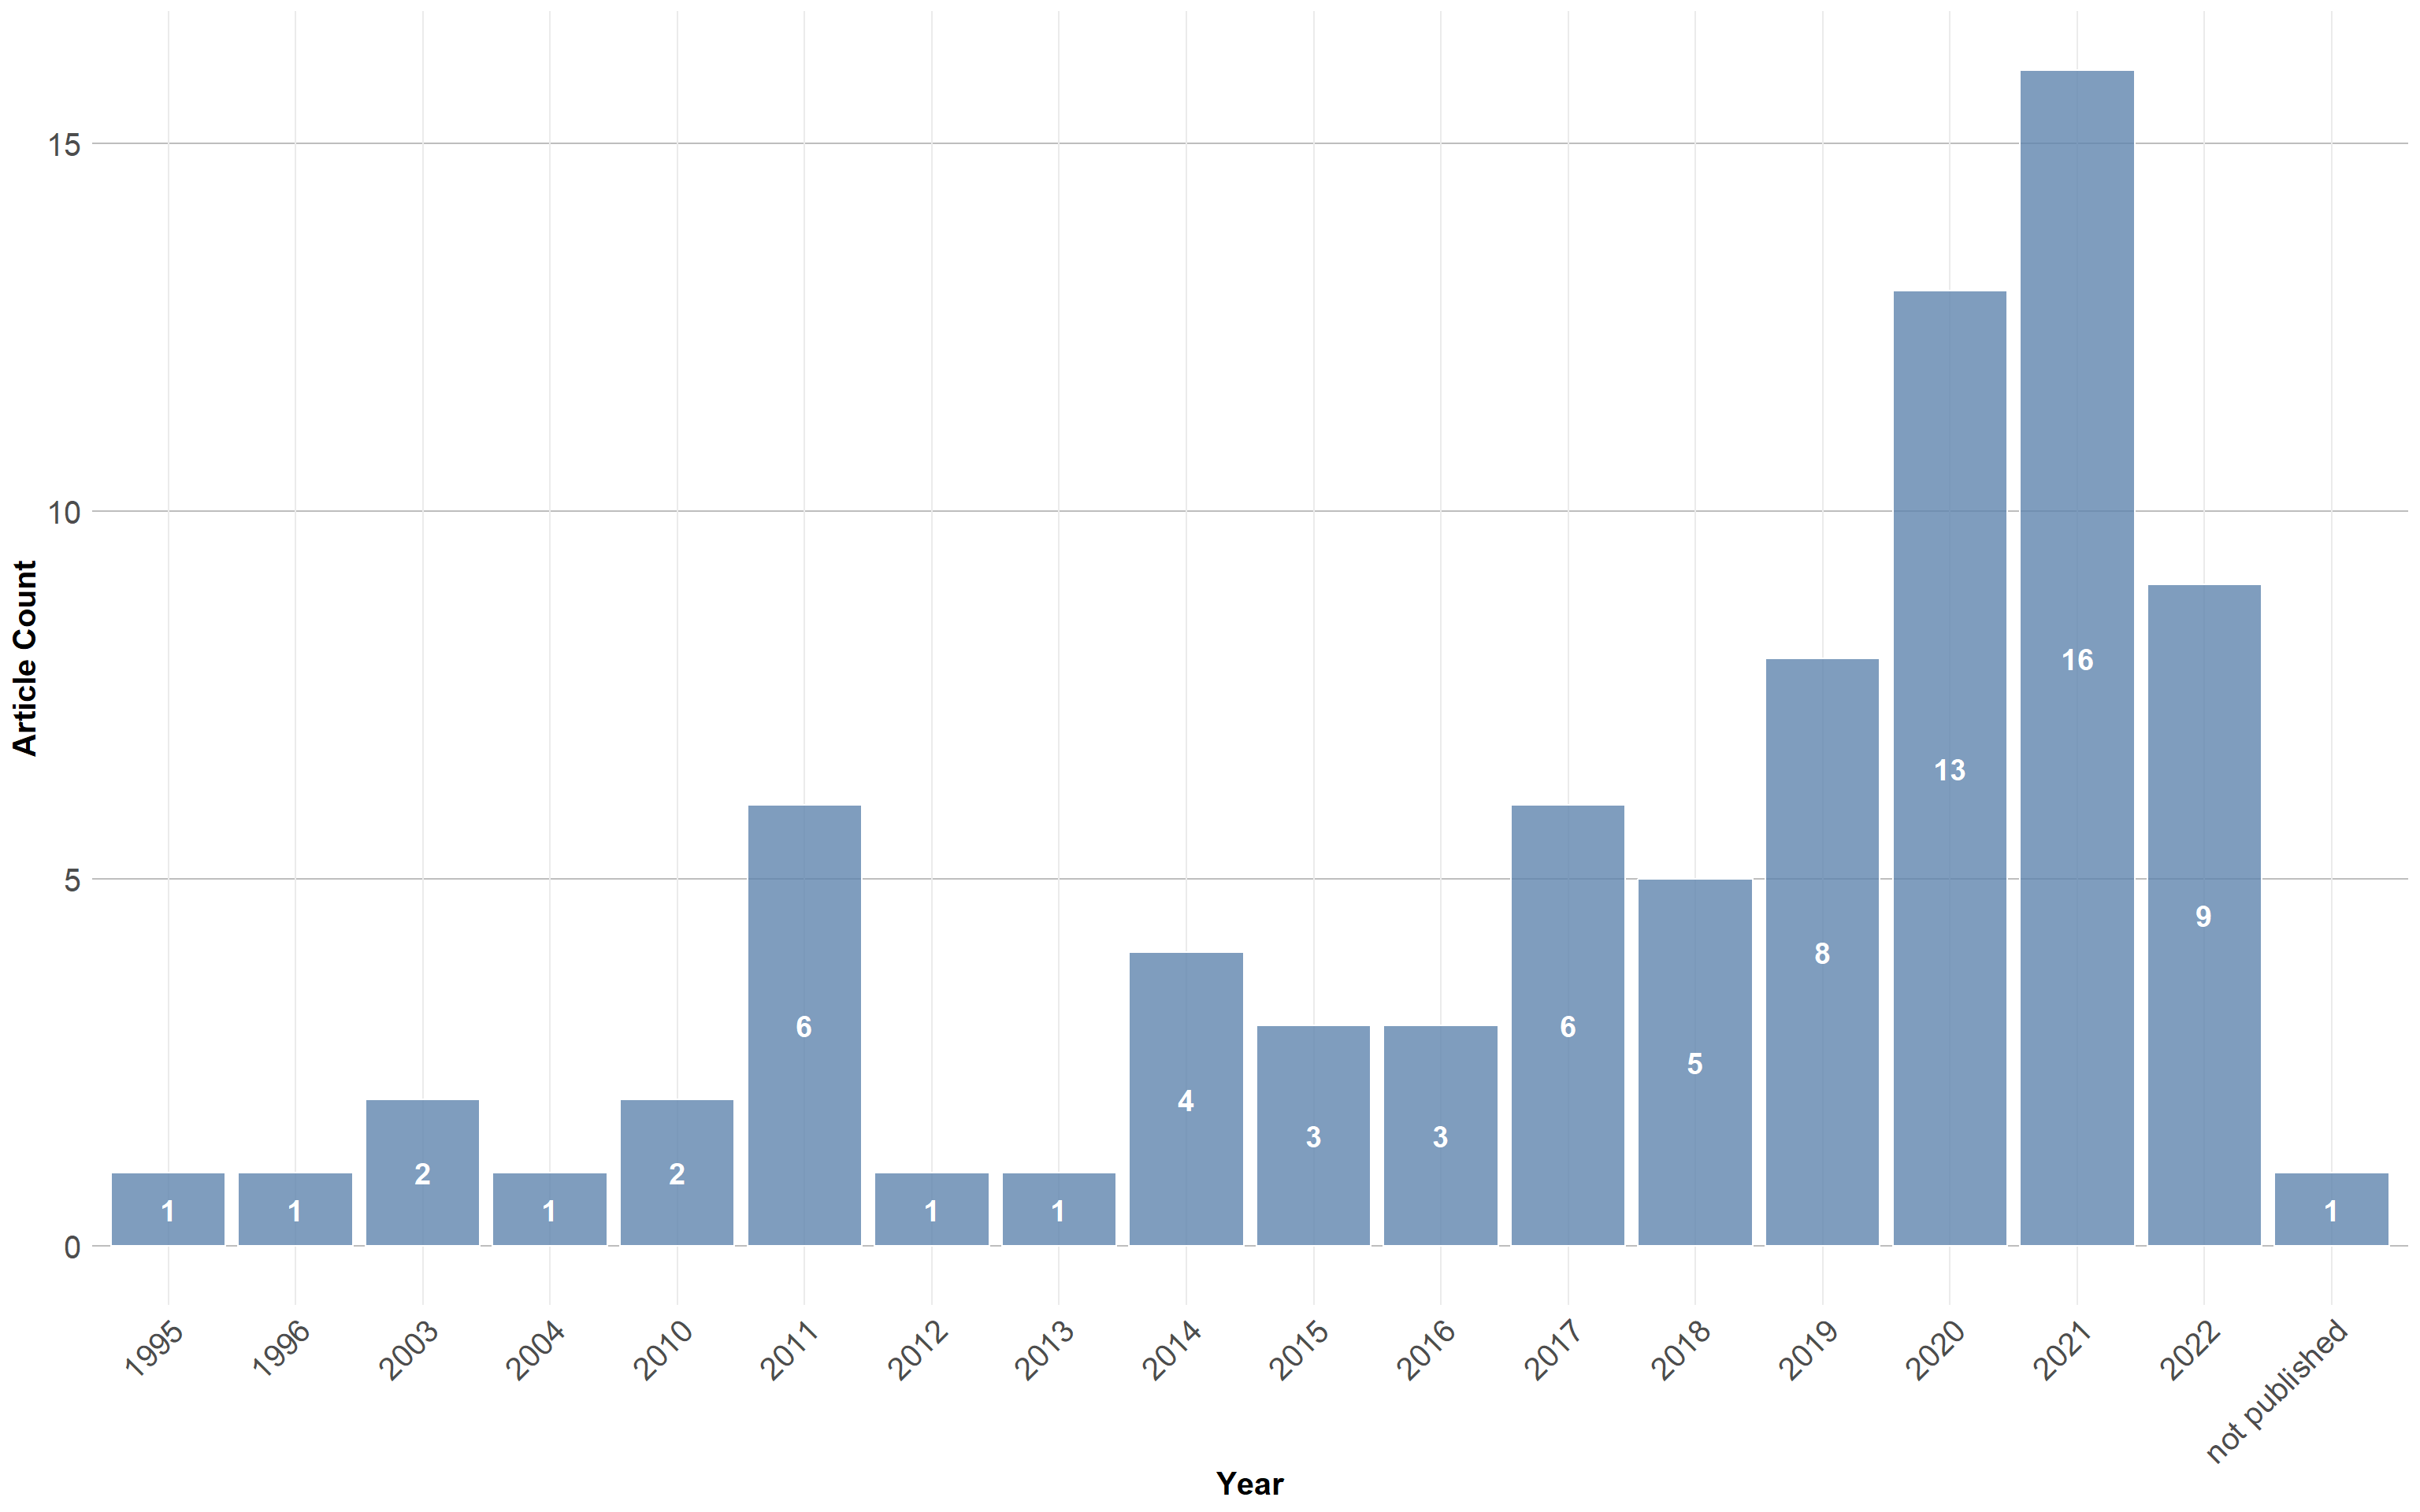
\includegraphics{zf_sm_code_files/figure-latex/unnamed-chunk-3-1.pdf}

\begin{Shaded}
\begin{Highlighting}[]
\CommentTok{\# ggsave(here("figures", "fig2\_time\_trends.pdf"), width = 16, height = 10, units = "cm", scale = 2, dpi = 300, device = cairo\_pdf)}
\end{Highlighting}
\end{Shaded}

\hypertarget{objective-1.-to-investigate-the-types-of-pesticides-and-pesticide-classes-both-in-terms-of-chemical-and-target-that-have-been-used-in-experiments-examining-the-effects-of-pesticide-exposure-on-zebrafish-behaviour.}{%
\section{Objective 1. To investigate the types of pesticides and
pesticide classes, both in terms of chemical and target, that have been
used in experiments examining the effects of pesticide exposure on
zebrafish
behaviour.}\label{objective-1.-to-investigate-the-types-of-pesticides-and-pesticide-classes-both-in-terms-of-chemical-and-target-that-have-been-used-in-experiments-examining-the-effects-of-pesticide-exposure-on-zebrafish-behaviour.}}

\hypertarget{fig3a---plot-for-total-of-individual-pesticides-used-in-pesticide-exposure-studies}{%
\subsection{fig3a - plot for total of individual pesticides used in
pesticide exposure
studies}\label{fig3a---plot-for-total-of-individual-pesticides-used-in-pesticide-exposure-studies}}

\begin{Shaded}
\begin{Highlighting}[]
\CommentTok{\# Separate rows with multiple pesticides, count their occurrence, and combined all pesticide that occured once as "other"}
\NormalTok{total\_pesticide\_count }\OtherTok{\textless{}{-}}\NormalTok{ pd }\SpecialCharTok{\%\textgreater{}\%}
  \FunctionTok{separate\_rows}\NormalTok{(pesticide\_investigated, }\AttributeTok{sep =} \StringTok{", "}\NormalTok{) }\SpecialCharTok{\%\textgreater{}\%}
  \FunctionTok{count}\NormalTok{(pesticide\_investigated) }\SpecialCharTok{\%\textgreater{}\%}
  \FunctionTok{mutate}\NormalTok{(}\AttributeTok{pesticide\_investigated =} \FunctionTok{ifelse}\NormalTok{(n }\SpecialCharTok{==} \DecValTok{1}\NormalTok{, }\StringTok{"other"}\NormalTok{, }\FunctionTok{as.character}\NormalTok{(pesticide\_investigated))) }\SpecialCharTok{\%\textgreater{}\%}
  \CommentTok{\# "other" includes tribotyltin, terbutylazine, sodium fluride, pyrimethonil, pyraclostrobin, propiconazole, prochloraz, parathion, paclobutazol, monocotophos, methylbenzoate, methylbenzoate, methomyl, mecroprop, linuron, endosulfan, diuron, difenoconazole, dicamba,   cyprodinil, chlorothalonil, carbofuran, carbaryl, broflanilide and boscalid. }
  \FunctionTok{group\_by}\NormalTok{(pesticide\_investigated) }\SpecialCharTok{\%\textgreater{}\%}
  \FunctionTok{summarise}\NormalTok{(}\AttributeTok{n =} \FunctionTok{sum}\NormalTok{(n))}

  \CommentTok{\# Calculate pesticide count as a percentage }
\NormalTok{  pesticide\_pct }\OtherTok{\textless{}{-}}\NormalTok{ total\_pesticide\_count }\SpecialCharTok{\%\textgreater{}\%}
  \FunctionTok{mutate}\NormalTok{(}\AttributeTok{proportion =}\NormalTok{ n}\SpecialCharTok{/}\FunctionTok{sum}\NormalTok{(total\_pesticide\_count}\SpecialCharTok{$}\NormalTok{n),}
         \AttributeTok{percentage =}\NormalTok{ proportion}\SpecialCharTok{*}\DecValTok{100}\NormalTok{)}
  
\CommentTok{\# Create a bar chart with the count of pesticides on the x{-}axis and pesticides on the y{-}axis}
\NormalTok{fig3a }\OtherTok{\textless{}{-}}  \FunctionTok{ggplot}\NormalTok{(pesticide\_pct, }\FunctionTok{aes}\NormalTok{(}\AttributeTok{x =} \FunctionTok{reorder}\NormalTok{(pesticide\_investigated, n), }\AttributeTok{y =}\NormalTok{ percentage)) }\SpecialCharTok{+}
  
  \CommentTok{\# Customize the appearance of the bars}
  \FunctionTok{geom\_bar}\NormalTok{(}\AttributeTok{stat =} \StringTok{"identity"}\NormalTok{, }\AttributeTok{fill =} \StringTok{"\#5F85AE"}\NormalTok{, }\AttributeTok{color =} \StringTok{"white"}\NormalTok{, }\AttributeTok{alpha =} \FloatTok{0.8}\NormalTok{, }\AttributeTok{position =} \FunctionTok{position\_dodge}\NormalTok{(}\FloatTok{0.9}\NormalTok{)) }\SpecialCharTok{+}
  
  \CommentTok{\# Add labels to the bars for absolute count }
  \FunctionTok{geom\_text}\NormalTok{(}\FunctionTok{aes}\NormalTok{(}\AttributeTok{label =}\NormalTok{ n), }\AttributeTok{position =} \FunctionTok{position\_stack}\NormalTok{(}\AttributeTok{vjust =} \FloatTok{0.5}\NormalTok{), }\AttributeTok{color =} \StringTok{"white"}\NormalTok{, }\AttributeTok{fontface =} \StringTok{"bold"}\NormalTok{, }\AttributeTok{size =} \DecValTok{5}\NormalTok{) }\SpecialCharTok{+}
  

  \CommentTok{\# Add labels to the bars for percentage }
 \FunctionTok{geom\_text}\NormalTok{(}\AttributeTok{data =}\NormalTok{ pesticide\_pct, }\FunctionTok{aes}\NormalTok{(}\AttributeTok{label =} \FunctionTok{paste0}\NormalTok{(}\FunctionTok{round}\NormalTok{(percentage,}\DecValTok{1}\NormalTok{), }\StringTok{"\%"}\NormalTok{)), }
            \AttributeTok{position =} \FunctionTok{position\_dodge}\NormalTok{(}\AttributeTok{width =} \FloatTok{0.9}\NormalTok{), }\AttributeTok{hjust =} \SpecialCharTok{{-}}\FloatTok{0.2}\NormalTok{, }\AttributeTok{size =} \DecValTok{5}\NormalTok{, }\AttributeTok{color =} \StringTok{"black"}\NormalTok{, }\AttributeTok{fontface =} \StringTok{"bold"}\NormalTok{) }\SpecialCharTok{+}
  
  \CommentTok{\# Customize the appearance of the plot}
  \FunctionTok{labs}\NormalTok{(}\AttributeTok{x =} \StringTok{"Pesticide"}\NormalTok{, }\AttributeTok{y =} \StringTok{"Percentage"}\NormalTok{) }\SpecialCharTok{+}
  \FunctionTok{theme\_minimal}\NormalTok{() }\SpecialCharTok{+}
  \FunctionTok{theme}\NormalTok{(}\AttributeTok{panel.grid.major.y =} \FunctionTok{element\_blank}\NormalTok{(),}
        \AttributeTok{axis.line.y =} \FunctionTok{element\_blank}\NormalTok{(),}
        \AttributeTok{axis.ticks.y =} \FunctionTok{element\_blank}\NormalTok{(),}
        \AttributeTok{axis.title.x =} \FunctionTok{element\_text}\NormalTok{(}\AttributeTok{size =} \DecValTok{15}\NormalTok{),}
        \AttributeTok{axis.title.y =} \FunctionTok{element\_text}\NormalTok{(}\AttributeTok{size =} \DecValTok{15}\NormalTok{),}
        \AttributeTok{axis.text.x =} \FunctionTok{element\_text}\NormalTok{(}\AttributeTok{size =} \DecValTok{15}\NormalTok{),}
        \AttributeTok{axis.text.y =} \FunctionTok{element\_text}\NormalTok{(}\AttributeTok{size =} \DecValTok{15}\NormalTok{),}
        \AttributeTok{axis.title =} \FunctionTok{element\_text}\NormalTok{(}\AttributeTok{size =} \DecValTok{15}\NormalTok{),}
        \AttributeTok{plot.title =} \FunctionTok{element\_blank}\NormalTok{()) }\SpecialCharTok{+}
        \FunctionTok{coord\_flip}\NormalTok{() }\SpecialCharTok{+}
        \FunctionTok{ylim}\NormalTok{(}\DecValTok{0}\NormalTok{,}\DecValTok{30}\NormalTok{)}


\NormalTok{ fig3a}
\end{Highlighting}
\end{Shaded}

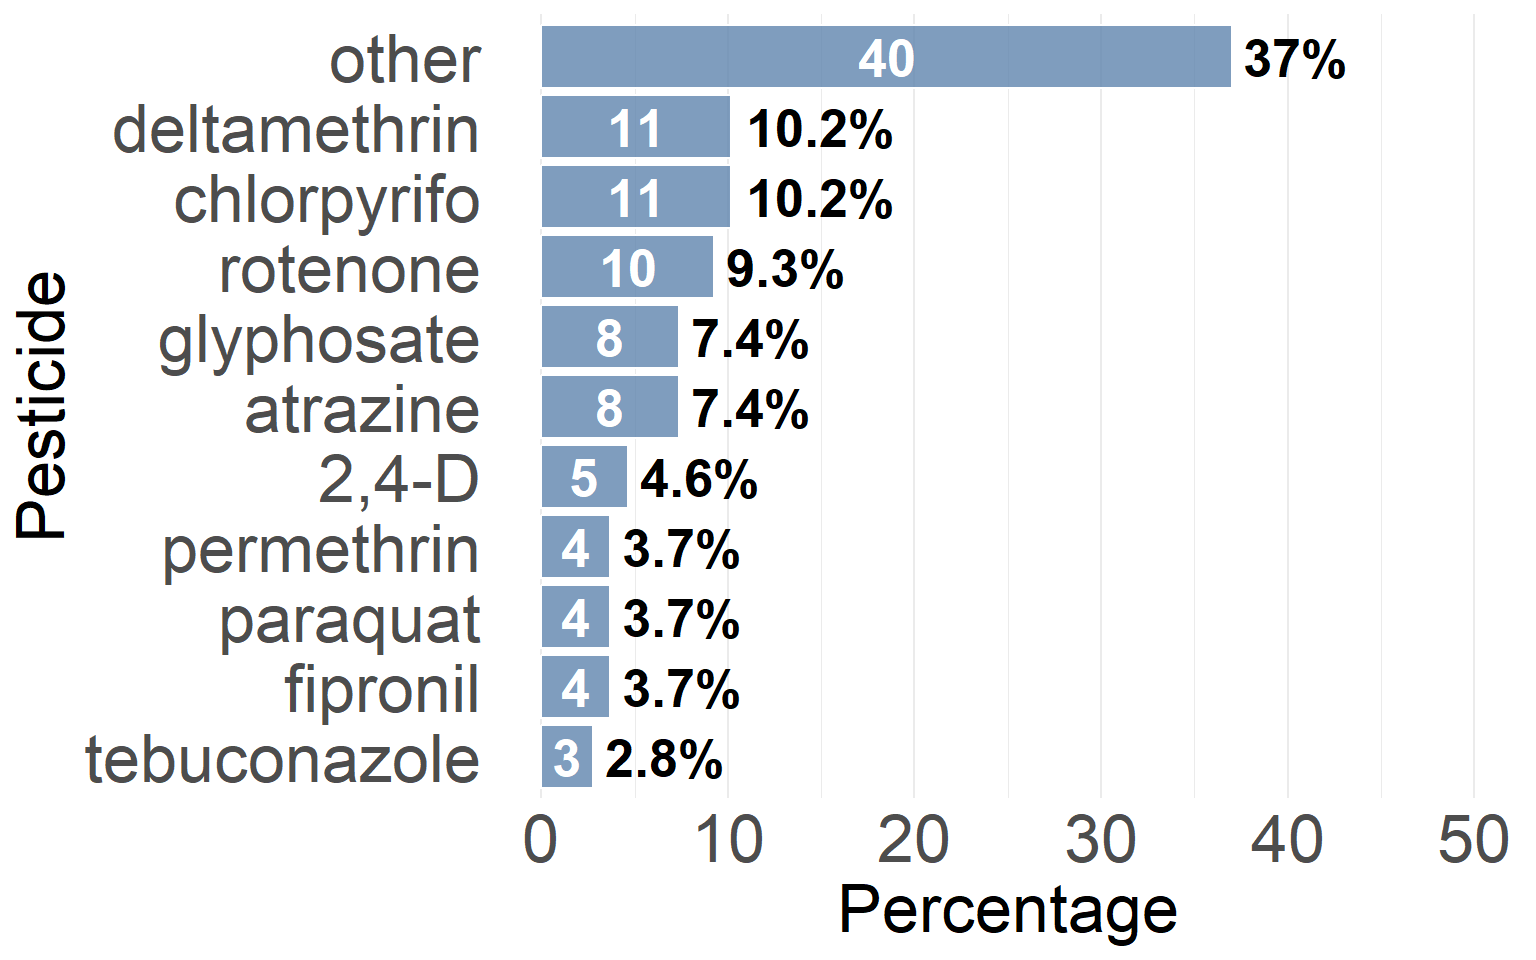
\includegraphics{zf_sm_code_files/figure-latex/unnamed-chunk-4-1.pdf}

\begin{Shaded}
\begin{Highlighting}[]
\CommentTok{\# ggsave(here("figures", "fig3a\_pesticide\_count.pdf"), width = 16, height = 10, units = "cm", scale = 2, dpi = 300, device = cairo\_pdf)}
\end{Highlighting}
\end{Shaded}

\hypertarget{fig3b---total-for-each-pesticide-target-class-used-in-pesticide-exposure-studies}{%
\subsection{fig3b - total for each pesticide target class used in
pesticide exposure
studies}\label{fig3b---total-for-each-pesticide-target-class-used-in-pesticide-exposure-studies}}

\begin{Shaded}
\begin{Highlighting}[]
\CommentTok{\# Separate rows with multiple pesticides and count their occurrence}
\NormalTok{total\_target\_class\_count }\OtherTok{\textless{}{-}}\NormalTok{ pd }\SpecialCharTok{\%\textgreater{}\%}
  \FunctionTok{separate\_rows}\NormalTok{(pesticide\_target\_class, }\AttributeTok{sep =} \StringTok{",}\SpecialCharTok{\textbackslash{}\textbackslash{}}\StringTok{s*"}\NormalTok{) }\SpecialCharTok{\%\textgreater{}\%}  
  \FunctionTok{count}\NormalTok{(pesticide\_target\_class) }

\CommentTok{\# Calculate target class count as a percentage }
\NormalTok{  target\_class\_pct }\OtherTok{\textless{}{-}}\NormalTok{ total\_target\_class\_count }\SpecialCharTok{\%\textgreater{}\%}
  \FunctionTok{mutate}\NormalTok{(}\AttributeTok{proportion =}\NormalTok{ n}\SpecialCharTok{/}\FunctionTok{sum}\NormalTok{(total\_target\_class\_count}\SpecialCharTok{$}\NormalTok{n),}
         \AttributeTok{percentage =}\NormalTok{ proportion}\SpecialCharTok{*}\DecValTok{100}\NormalTok{)}
  
\CommentTok{\# Create a bar chart with the count of target classes  on the x{-}axis and pesticides target class  on the y{-}axis}
\NormalTok{fig3b }\OtherTok{\textless{}{-}} \FunctionTok{ggplot}\NormalTok{(target\_class\_pct, }\FunctionTok{aes}\NormalTok{(}\FunctionTok{reorder}\NormalTok{(pesticide\_target\_class, n), }\AttributeTok{y =}\NormalTok{ percentage)) }\SpecialCharTok{+}
  
  \CommentTok{\# Customize the appearance of the bars}
  \FunctionTok{geom\_bar}\NormalTok{(}\AttributeTok{stat =} \StringTok{"identity"}\NormalTok{, }\AttributeTok{fill =} \StringTok{"\#5F85AE"}\NormalTok{, }\AttributeTok{color =} \StringTok{"white"}\NormalTok{, }\AttributeTok{alpha =} \FloatTok{0.8}\NormalTok{, }\AttributeTok{position =} \FunctionTok{position\_dodge}\NormalTok{(}\FloatTok{0.9}\NormalTok{)) }\SpecialCharTok{+} 
  
  \CommentTok{\# Add labels to the bars for absolute count}
  \FunctionTok{geom\_text}\NormalTok{(}\FunctionTok{aes}\NormalTok{(}\AttributeTok{label =}\NormalTok{ n), }\AttributeTok{position =} \FunctionTok{position\_stack}\NormalTok{(}\AttributeTok{vjust =} \FloatTok{0.5}\NormalTok{), }\AttributeTok{color =} \StringTok{"white"}\NormalTok{, }\AttributeTok{fontface =} \StringTok{"bold"}\NormalTok{, }\AttributeTok{size =} \DecValTok{7}\NormalTok{) }\SpecialCharTok{+}
  
  \CommentTok{\# Add labels to the bars for percentage }
 \FunctionTok{geom\_text}\NormalTok{(}\AttributeTok{data =}\NormalTok{ target\_class\_pct, }\FunctionTok{aes}\NormalTok{(}\AttributeTok{label =} \FunctionTok{paste0}\NormalTok{(}\FunctionTok{round}\NormalTok{(percentage, }\DecValTok{1}\NormalTok{), }\StringTok{"\%"}\NormalTok{)), }
            \AttributeTok{position =} \FunctionTok{position\_dodge}\NormalTok{(}\AttributeTok{width =} \FloatTok{0.9}\NormalTok{), }\AttributeTok{hjust =} \SpecialCharTok{{-}}\FloatTok{0.2}\NormalTok{, }\AttributeTok{size =} \DecValTok{7}\NormalTok{, }\AttributeTok{color =} \StringTok{"black"}\NormalTok{, }\AttributeTok{fontface =} \StringTok{"bold"}\NormalTok{) }\SpecialCharTok{+}
    
  \CommentTok{\# Customize the appearance of the plot}
  \FunctionTok{labs}\NormalTok{(}\AttributeTok{x =} \StringTok{"Pesticide Target Class"}\NormalTok{, }\AttributeTok{y =} \StringTok{"Percentage"}\NormalTok{) }\SpecialCharTok{+}
  \FunctionTok{theme\_minimal}\NormalTok{() }\SpecialCharTok{+}
  \FunctionTok{theme}\NormalTok{(}\AttributeTok{panel.grid.major.y =} \FunctionTok{element\_blank}\NormalTok{(),}
    \AttributeTok{axis.line.y =} \FunctionTok{element\_blank}\NormalTok{(),}
    \AttributeTok{axis.ticks.y =} \FunctionTok{element\_blank}\NormalTok{(),}
    \AttributeTok{axis.text.x =} \FunctionTok{element\_text}\NormalTok{(}\AttributeTok{size =} \DecValTok{20}\NormalTok{),}
    \AttributeTok{axis.text.y =} \FunctionTok{element\_text}\NormalTok{(}\AttributeTok{size =} \DecValTok{20}\NormalTok{),}
    \AttributeTok{axis.title.x =} \FunctionTok{element\_text}\NormalTok{(}\AttributeTok{size =} \DecValTok{20}\NormalTok{),}
    \AttributeTok{axis.title.y =} \FunctionTok{element\_text}\NormalTok{(}\AttributeTok{size =} \DecValTok{20}\NormalTok{),}
    \AttributeTok{plot.title =} \FunctionTok{element\_blank}\NormalTok{()) }\SpecialCharTok{+}
    \FunctionTok{coord\_flip}\NormalTok{() }\SpecialCharTok{+}
    \FunctionTok{ylim}\NormalTok{(}\DecValTok{0}\NormalTok{, }\DecValTok{80}\NormalTok{)}


\NormalTok{ fig3b}
\end{Highlighting}
\end{Shaded}

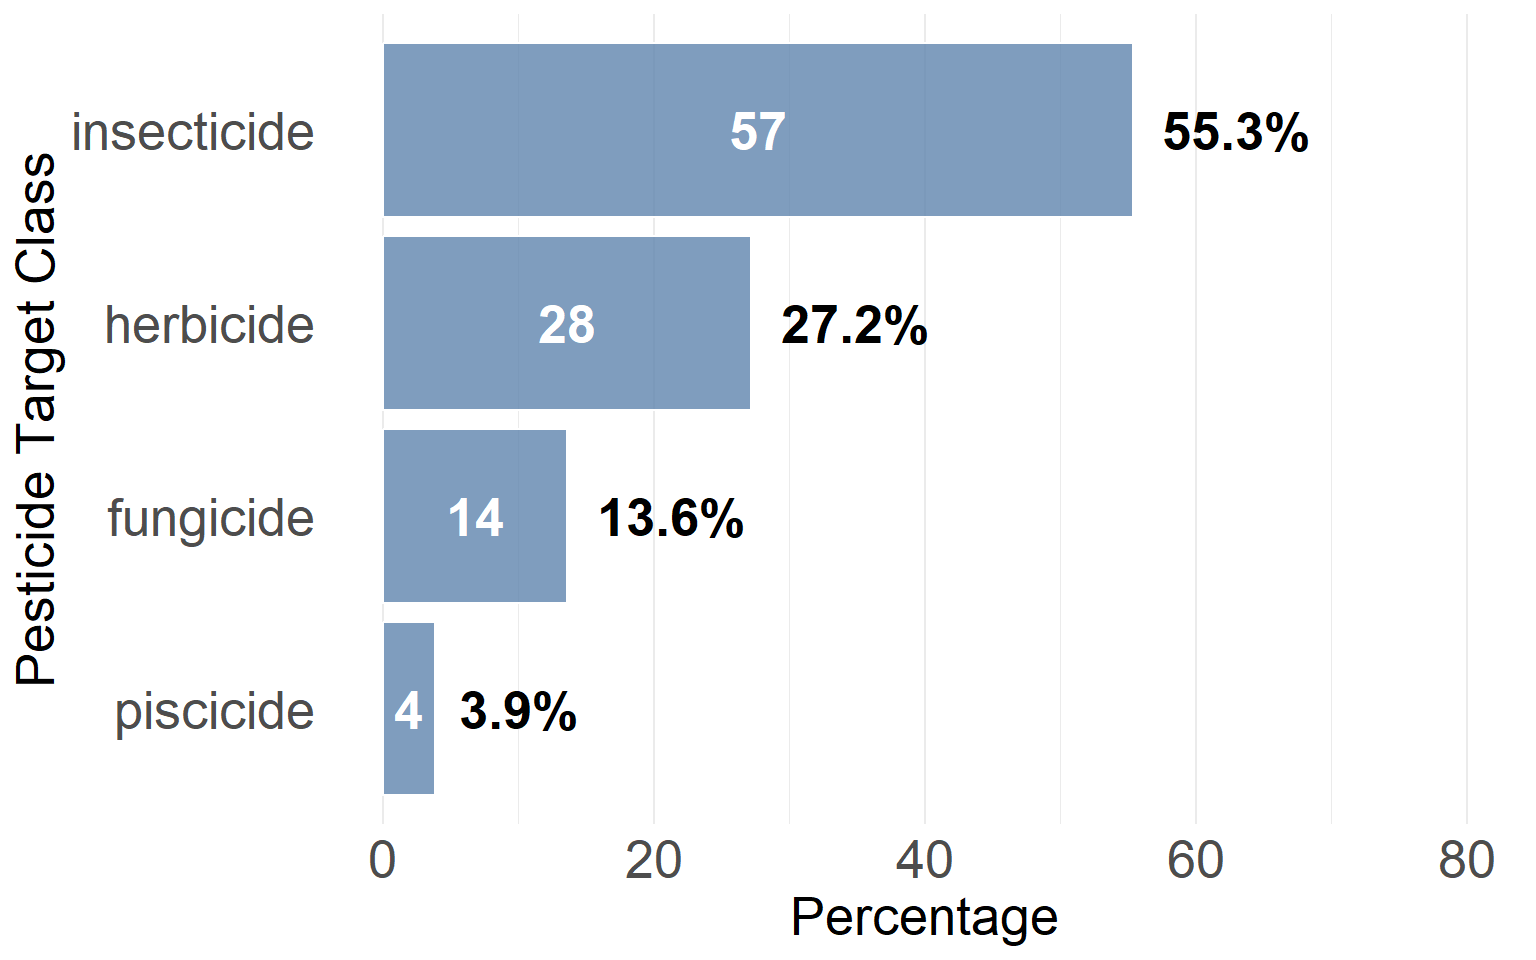
\includegraphics{zf_sm_code_files/figure-latex/unnamed-chunk-5-1.pdf}

\begin{Shaded}
\begin{Highlighting}[]
\CommentTok{\# ggsave(here("figures", "fig3b\_pesticide\_target\_count.pdf"), width = 16, height = 10, units = "cm", scale = 2, dpi = 300, device = cairo\_pdf)}
\end{Highlighting}
\end{Shaded}

\hypertarget{fig3c---total-for-chemical-class}{%
\subsection{fig3c - total for chemical
class}\label{fig3c---total-for-chemical-class}}

\begin{Shaded}
\begin{Highlighting}[]
\CommentTok{\# Separate rows with multiple pesticides and count their occurrence, then filter for cases with more than one occurrence}
\NormalTok{total\_chemical\_class\_count }\OtherTok{\textless{}{-}}\NormalTok{ pd }\SpecialCharTok{\%\textgreater{}\%}
  \FunctionTok{separate\_rows}\NormalTok{(pesticide\_chemical\_class, }\AttributeTok{sep =} \StringTok{",}\SpecialCharTok{\textbackslash{}\textbackslash{}}\StringTok{s*"}\NormalTok{) }\SpecialCharTok{\%\textgreater{}\%}  
  \FunctionTok{count}\NormalTok{(pesticide\_chemical\_class) }\SpecialCharTok{\%\textgreater{}\%}
    \FunctionTok{mutate}\NormalTok{(}\AttributeTok{pesticide\_chemical\_class =} \FunctionTok{ifelse}\NormalTok{(n }\SpecialCharTok{==} \DecValTok{1}\NormalTok{, }\StringTok{"other"}\NormalTok{, }\FunctionTok{as.character}\NormalTok{(pesticide\_chemical\_class))) }\SpecialCharTok{\%\textgreater{}\%}
  \CommentTok{\# "other" includes tribotyltin, terbutylazine, sodium fluride, pyrimethonil, pyraclostrobin, propiconazole, prochloraz, parathion,       paclobutazol, monocotophos, methylbenzoate, methylbenzoate, methomyl, mecroprop, linuron, endosulfan, diuron, difenoconazole, dicamba,   cyprodinil, chlorothalonil, carbofuran, carbaryl, broflanilide and boscalid. }
  \FunctionTok{group\_by}\NormalTok{(pesticide\_chemical\_class) }\SpecialCharTok{\%\textgreater{}\%}
  \FunctionTok{summarise}\NormalTok{(}\AttributeTok{n =} \FunctionTok{sum}\NormalTok{(n))}

\CommentTok{\# Calculate target class count as a percentage }
\NormalTok{  chemical\_class\_pct }\OtherTok{\textless{}{-}}\NormalTok{ total\_chemical\_class\_count }\SpecialCharTok{\%\textgreater{}\%}
  \FunctionTok{mutate}\NormalTok{(}\AttributeTok{proportion =}\NormalTok{ n}\SpecialCharTok{/}\FunctionTok{sum}\NormalTok{(total\_chemical\_class\_count}\SpecialCharTok{$}\NormalTok{n),}
         \AttributeTok{percentage =}\NormalTok{ proportion}\SpecialCharTok{*}\DecValTok{100}\NormalTok{)}
  
  \CommentTok{\# Create a bar chart with the count of chemical classes on the x{-}axis and pesticides chemical class on the y{-}axis}
\NormalTok{ fig3c }\OtherTok{\textless{}{-}}  \FunctionTok{ggplot}\NormalTok{(chemical\_class\_pct, }\FunctionTok{aes}\NormalTok{(}\AttributeTok{x =} \FunctionTok{reorder}\NormalTok{(pesticide\_chemical\_class,n), }\AttributeTok{y =}\NormalTok{ percentage)) }\SpecialCharTok{+}
  
  \CommentTok{\# Customize the appearance of the bars}
  \FunctionTok{geom\_bar}\NormalTok{(}\AttributeTok{stat =} \StringTok{"identity"}\NormalTok{, }\AttributeTok{fill =} \StringTok{"\#5F85AE"}\NormalTok{, }\AttributeTok{color =} \StringTok{"white"}\NormalTok{, }\AttributeTok{alpha =} \FloatTok{0.8}\NormalTok{, }\AttributeTok{position =} \FunctionTok{position\_dodge}\NormalTok{(}\FloatTok{0.9}\NormalTok{)) }\SpecialCharTok{+}
  
  \CommentTok{\# Add labels to the bars}
  \FunctionTok{geom\_text}\NormalTok{(}\FunctionTok{aes}\NormalTok{(}\AttributeTok{label =}\NormalTok{ n), }\AttributeTok{position =} \FunctionTok{position\_stack}\NormalTok{(}\AttributeTok{vjust =} \FloatTok{0.5}\NormalTok{), }\AttributeTok{color =} \StringTok{"white"}\NormalTok{, }\AttributeTok{fontface =} \StringTok{"bold"}\NormalTok{, }\AttributeTok{size =} \DecValTok{5}\NormalTok{) }\SpecialCharTok{+}
  
   
  \CommentTok{\# Add labels to the bars for percentage }
 \FunctionTok{geom\_text}\NormalTok{(}\AttributeTok{data =}\NormalTok{ chemical\_class\_pct, }\FunctionTok{aes}\NormalTok{(}\AttributeTok{label =} \FunctionTok{paste0}\NormalTok{(}\FunctionTok{round}\NormalTok{(percentage,}\DecValTok{1}\NormalTok{), }\StringTok{"\%"}\NormalTok{)), }
            \AttributeTok{position =} \FunctionTok{position\_dodge}\NormalTok{(}\AttributeTok{width =} \FloatTok{0.9}\NormalTok{), }\AttributeTok{hjust =} \SpecialCharTok{{-}}\FloatTok{0.2}\NormalTok{, }\AttributeTok{size =} \DecValTok{5}\NormalTok{, }\AttributeTok{color =} \StringTok{"black"}\NormalTok{, }\AttributeTok{fontface =} \StringTok{"bold"}\NormalTok{) }\SpecialCharTok{+}
   
  \CommentTok{\# Customize the appearance of the plot}
  \FunctionTok{labs}\NormalTok{(}\AttributeTok{x =} \StringTok{"Pesticide Chemical Class"}\NormalTok{, }\AttributeTok{y =} \StringTok{"Percentage"}\NormalTok{) }\SpecialCharTok{+}
  \FunctionTok{theme\_minimal}\NormalTok{() }\SpecialCharTok{+}
  \FunctionTok{theme}\NormalTok{(}\AttributeTok{panel.grid.major.y =} \FunctionTok{element\_blank}\NormalTok{(),}
    \AttributeTok{axis.line.y =} \FunctionTok{element\_blank}\NormalTok{(),}
    \AttributeTok{axis.ticks.y =} \FunctionTok{element\_blank}\NormalTok{(),}
    \AttributeTok{axis.text.x =} \FunctionTok{element\_text}\NormalTok{(}\AttributeTok{size =} \DecValTok{20}\NormalTok{),}
    \AttributeTok{axis.text.y =} \FunctionTok{element\_text}\NormalTok{(}\AttributeTok{size =} \DecValTok{15}\NormalTok{),}
    \AttributeTok{axis.title.x =} \FunctionTok{element\_text}\NormalTok{(}\AttributeTok{size =} \DecValTok{20}\NormalTok{),}
    \AttributeTok{axis.title.y =} \FunctionTok{element\_text}\NormalTok{(}\AttributeTok{size =} \DecValTok{20}\NormalTok{),}
    \AttributeTok{plot.title =} \FunctionTok{element\_blank}\NormalTok{()) }\SpecialCharTok{+}
    \FunctionTok{coord\_flip}\NormalTok{() }\SpecialCharTok{+}
    \FunctionTok{ylim}\NormalTok{(}\DecValTok{0}\NormalTok{, }\DecValTok{40}\NormalTok{)}
    

\NormalTok{ fig3c}
\end{Highlighting}
\end{Shaded}

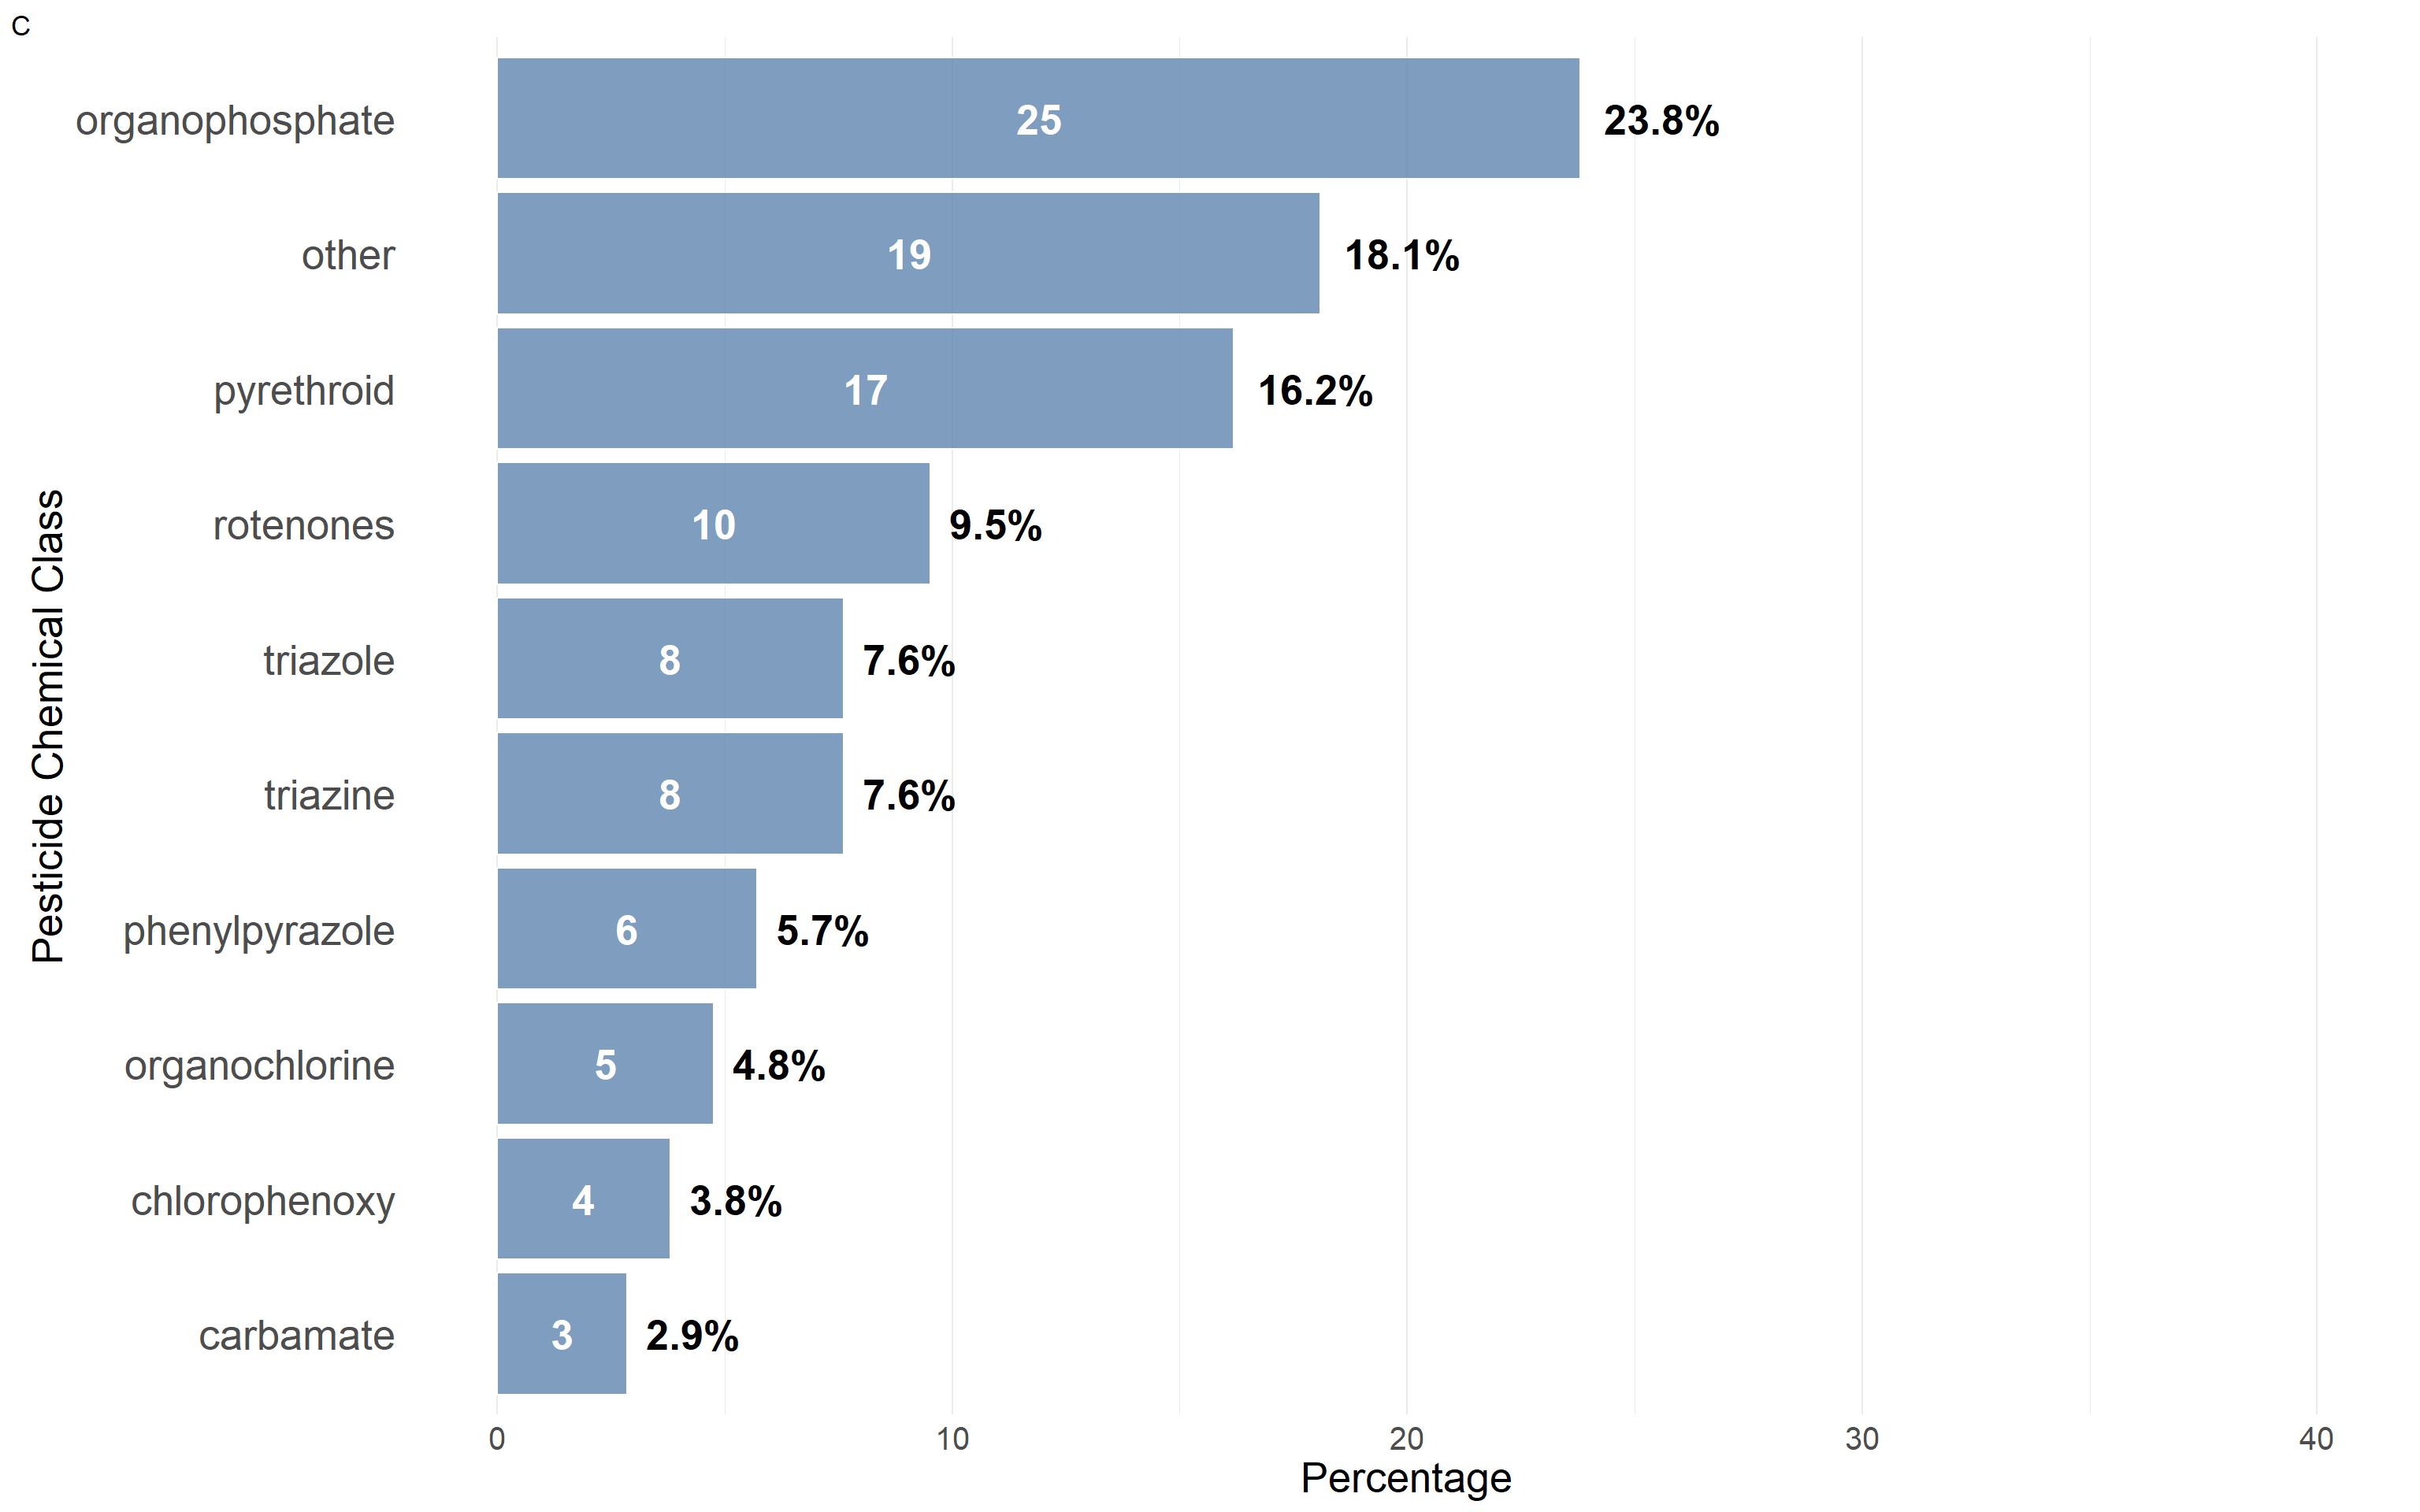
\includegraphics{zf_sm_code_files/figure-latex/unnamed-chunk-6-1.pdf}

\begin{Shaded}
\begin{Highlighting}[]
\CommentTok{\# ggsave(here("figures", "fig3c\_pesticide\_chemical\_count.pdf"), width = 16, height = 10, units = "cm", scale = 2, dpi = 300, device = cairo\_pdf)}
\end{Highlighting}
\end{Shaded}

\#\#fig3 combined

\begin{Shaded}
\begin{Highlighting}[]
\CommentTok{\# Combine three plots into a single plot using a grid layout}
\NormalTok{fig3 }\OtherTok{\textless{}{-}}\NormalTok{ ((fig3a) }\SpecialCharTok{|}\NormalTok{ (fig3b }\SpecialCharTok{/}\NormalTok{ fig3c) }\SpecialCharTok{+} \FunctionTok{plot\_annotation}\NormalTok{(}\AttributeTok{tag\_levels =} \StringTok{"A"}\NormalTok{))}

\NormalTok{fig3}
\end{Highlighting}
\end{Shaded}

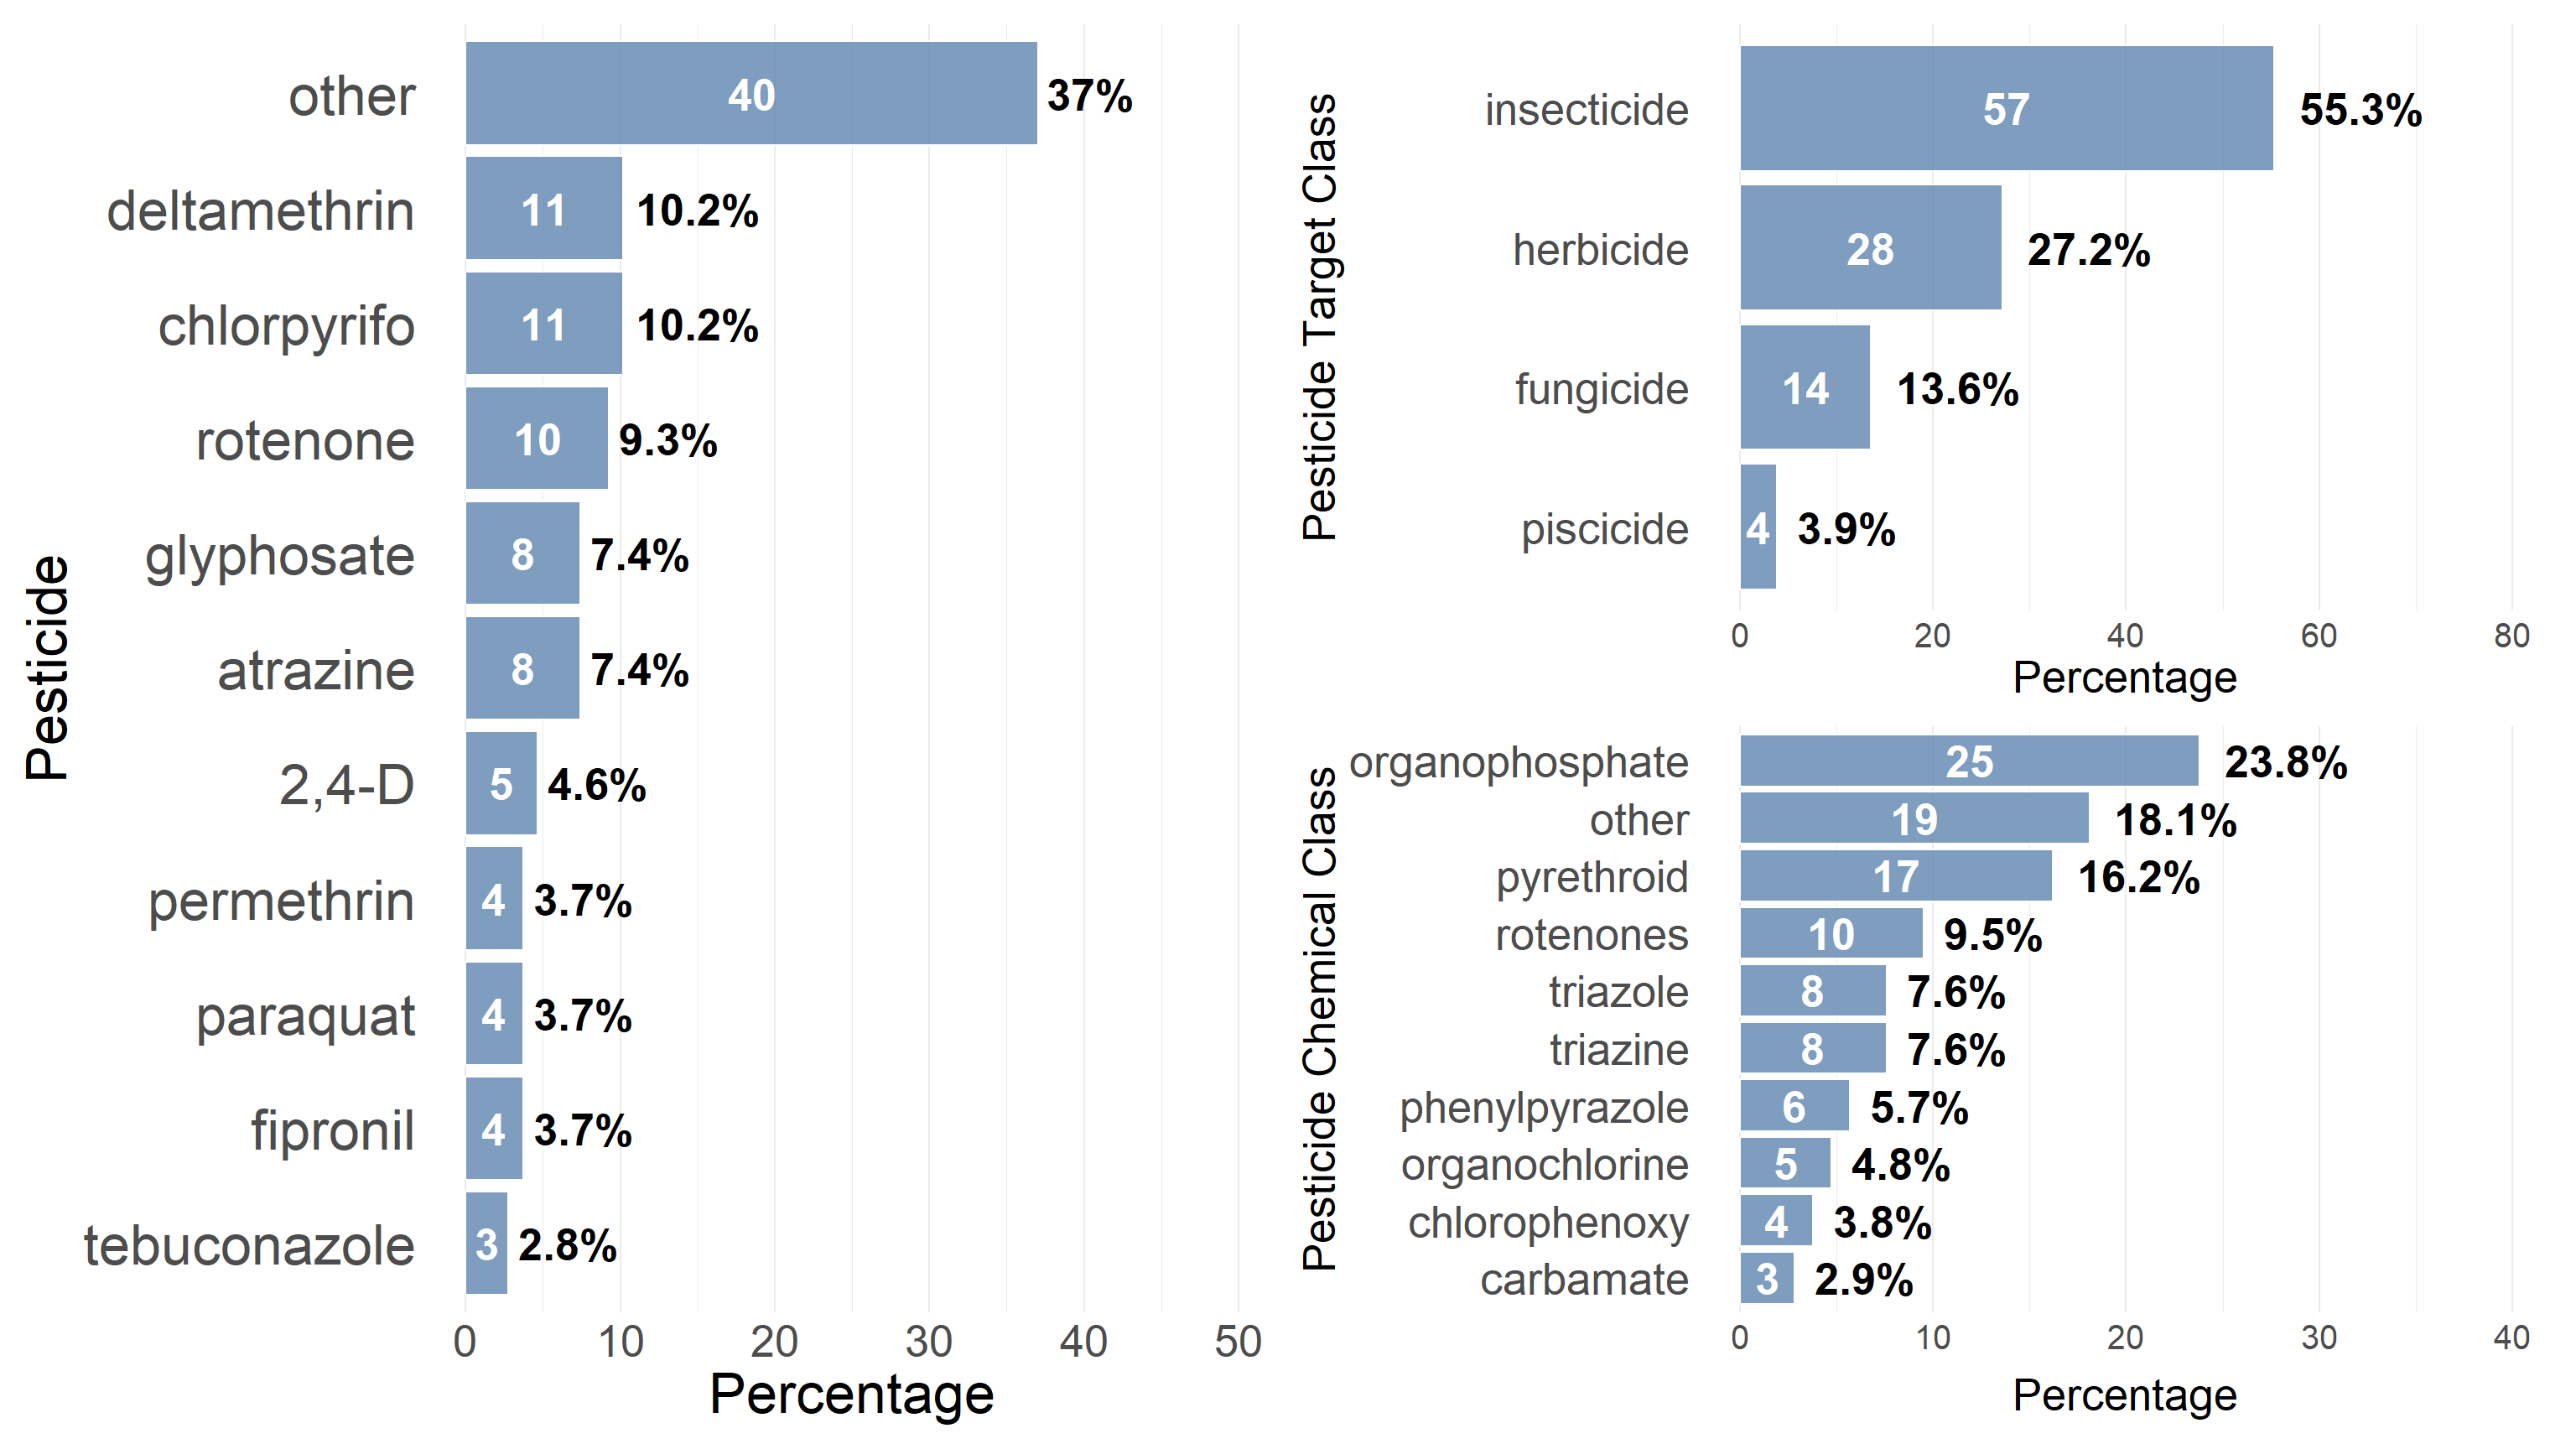
\includegraphics{zf_sm_code_files/figure-latex/unnamed-chunk-7-1.pdf}

\begin{Shaded}
\begin{Highlighting}[]
\CommentTok{\#ggsave(here("figures", "fig3\_pesticide\_count\_combined.pdf"), width = 16, height = 10, units = "cm", scale = 2, dpi = 300, device = cairo\_pdf)}
\end{Highlighting}
\end{Shaded}

Objective 2. To investigate pesticide exposure study designs such as
concentration and duration of exposure, life stages of zebrafish used in
each study and the sample sizes used.

\hypertarget{figs3---total-route-of-exposure-completed-as-a-percentage}{%
\subsection{figs3 - total route of exposure completed as a
percentage}\label{figs3---total-route-of-exposure-completed-as-a-percentage}}

\begin{Shaded}
\begin{Highlighting}[]
\CommentTok{\# Count the total occurrence of each route in the data set}
\NormalTok{total\_route\_count }\OtherTok{\textless{}{-}}\NormalTok{ pdo }\SpecialCharTok{\%\textgreater{}\%} 
                     \FunctionTok{count}\NormalTok{(route)}

\CommentTok{\# Count the proportion and percentage of each route in the data set}
\NormalTok{route\_pct }\OtherTok{\textless{}{-}}\NormalTok{ pdo }\SpecialCharTok{\%\textgreater{}\%}
  \FunctionTok{count}\NormalTok{(route) }\SpecialCharTok{\%\textgreater{}\%}
  \FunctionTok{mutate}\NormalTok{(}\AttributeTok{proportion =}\NormalTok{ n}\SpecialCharTok{/}\FunctionTok{sum}\NormalTok{(total\_route\_count}\SpecialCharTok{$}\NormalTok{n),}
         \AttributeTok{percentage =}\NormalTok{ proportion}\SpecialCharTok{*}\DecValTok{100}\NormalTok{)}

\CommentTok{\# Create a bar chart with the percentage of pesticides by route of exposure on the x{-}axis and the routes of exposure on the y{-}axis}
\NormalTok{figs3 }\OtherTok{\textless{}{-}} \FunctionTok{ggplot}\NormalTok{(route\_pct, }\FunctionTok{aes}\NormalTok{(}\AttributeTok{x =} \FunctionTok{reorder}\NormalTok{(route, percentage), }\AttributeTok{y =}\NormalTok{ percentage)) }\SpecialCharTok{+}
  
  \CommentTok{\# Customize the appearance of the bars}
  \FunctionTok{geom\_bar}\NormalTok{(}\AttributeTok{stat =} \StringTok{"identity"}\NormalTok{, }\AttributeTok{fill =} \StringTok{"\#5F85AE"}\NormalTok{, }\AttributeTok{color =} \StringTok{"white"}\NormalTok{, }\AttributeTok{alpha =} \FloatTok{0.8}\NormalTok{, }\AttributeTok{position =} \FunctionTok{position\_dodge}\NormalTok{(}\FloatTok{0.9}\NormalTok{)) }\SpecialCharTok{+}
  
  \CommentTok{\# Add absolute count to bars}
  \FunctionTok{geom\_text}\NormalTok{(}\FunctionTok{aes}\NormalTok{(}\AttributeTok{label =}\NormalTok{ n), }\AttributeTok{position =} \FunctionTok{position\_stack}\NormalTok{(}\AttributeTok{vjust =} \FloatTok{0.5}\NormalTok{), }\AttributeTok{color =} \StringTok{"white"}\NormalTok{, }\AttributeTok{fontface =} \StringTok{"bold"}\NormalTok{, }\AttributeTok{size =} \DecValTok{5}\NormalTok{) }\SpecialCharTok{+}
  
  \CommentTok{\# Add percentage label to bars }
  \FunctionTok{geom\_text}\NormalTok{(}\FunctionTok{aes}\NormalTok{(}\AttributeTok{label =} \FunctionTok{paste0}\NormalTok{(}\FunctionTok{round}\NormalTok{(percentage, }\DecValTok{1}\NormalTok{), }\StringTok{"\%"}\NormalTok{)), }\AttributeTok{hjust =} \SpecialCharTok{{-}}\FloatTok{0.2}\NormalTok{, }\AttributeTok{vjust =} \FloatTok{0.5}\NormalTok{, }\AttributeTok{size =} \DecValTok{5}\NormalTok{, }\AttributeTok{fontface =} \StringTok{"bold"}\NormalTok{) }\SpecialCharTok{+}
  
  \CommentTok{\# Customize the appearance of the plot}
  \FunctionTok{labs}\NormalTok{(}\AttributeTok{x =} \StringTok{"Route of Exposure"}\NormalTok{, }\AttributeTok{y =} \StringTok{"Percentage"}\NormalTok{) }\SpecialCharTok{+}
  \FunctionTok{theme\_minimal}\NormalTok{() }\SpecialCharTok{+}
  \FunctionTok{theme}\NormalTok{(}\AttributeTok{panel.grid.major.y =} \FunctionTok{element\_blank}\NormalTok{(),}
        \AttributeTok{axis.text.x =} \FunctionTok{element\_text}\NormalTok{(}\AttributeTok{size =} \DecValTok{15}\NormalTok{),}
        \AttributeTok{axis.text.y =} \FunctionTok{element\_text}\NormalTok{(}\AttributeTok{size =} \DecValTok{15}\NormalTok{),}
        \AttributeTok{axis.title.x =} \FunctionTok{element\_text}\NormalTok{(}\AttributeTok{size =} \DecValTok{15}\NormalTok{),}
        \AttributeTok{axis.title.y =} \FunctionTok{element\_text}\NormalTok{(}\AttributeTok{size =} \DecValTok{15}\NormalTok{),}
        \AttributeTok{plot.title =} \FunctionTok{element\_blank}\NormalTok{()) }\SpecialCharTok{+}
        \FunctionTok{coord\_flip}\NormalTok{() }\SpecialCharTok{+} 
        \FunctionTok{ylim}\NormalTok{(}\DecValTok{0}\NormalTok{, }\DecValTok{100}\NormalTok{)}


\NormalTok{figs3}
\end{Highlighting}
\end{Shaded}

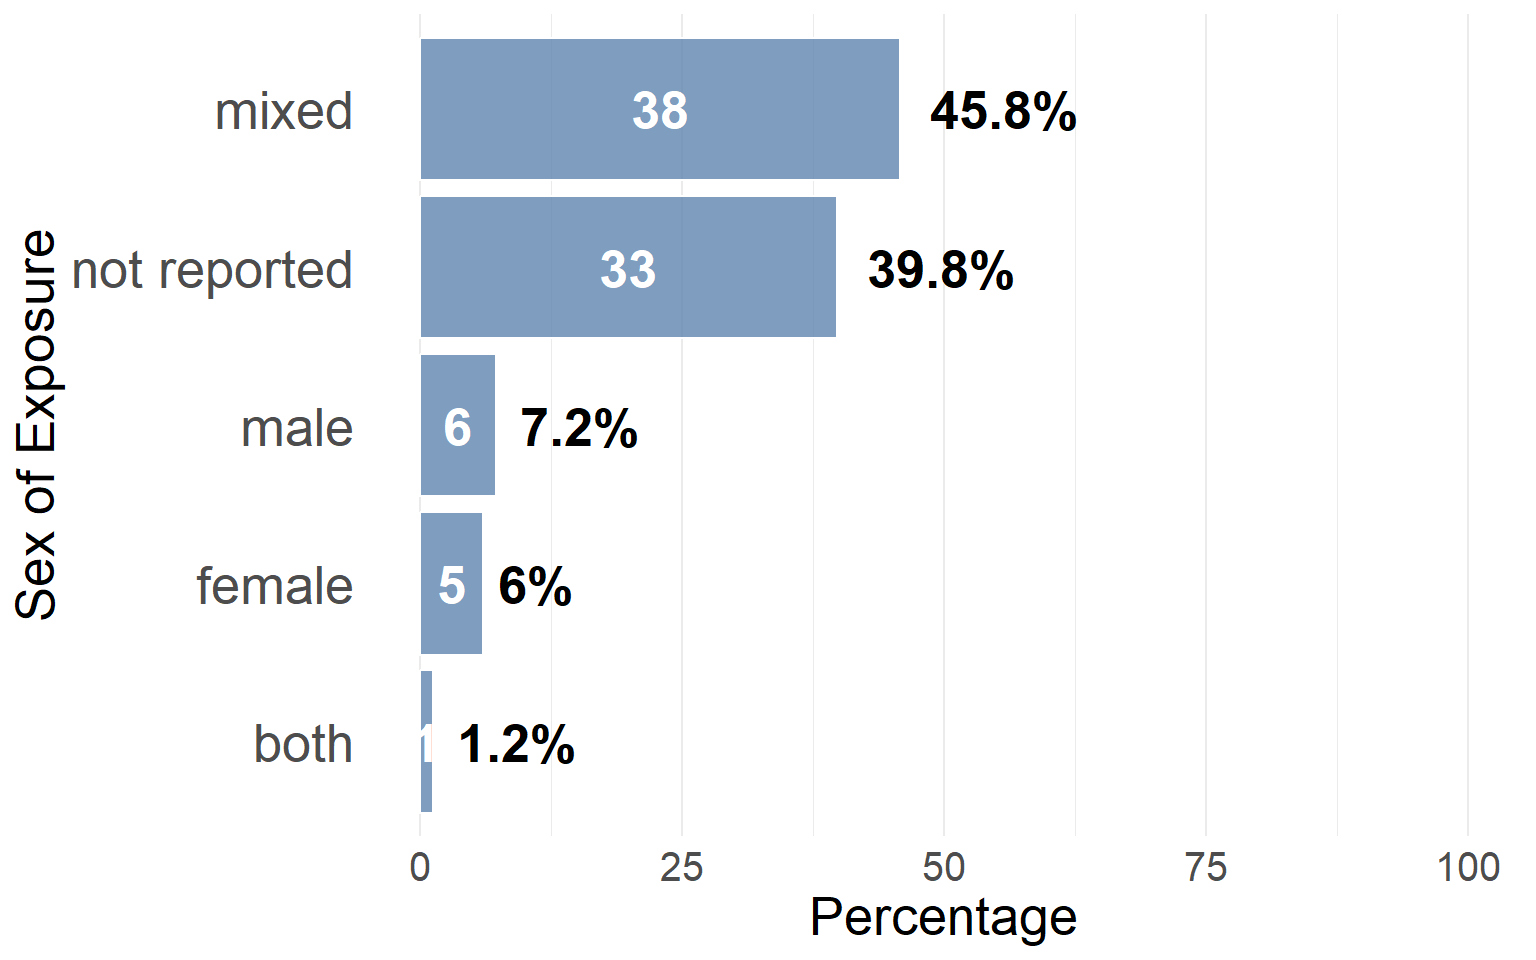
\includegraphics{zf_sm_code_files/figure-latex/unnamed-chunk-8-1.pdf}

\begin{Shaded}
\begin{Highlighting}[]
\CommentTok{\# ggsave(here("figures", "figs3\_pesticide\_chemical\_count.pdf"), width = 16, height = 10, units = "cm", scale = 2, dpi = 300, device = cairo\_pdf)}
\end{Highlighting}
\end{Shaded}

\hypertarget{objective-2.-to-investigate-the-study-designs-employed-to-assess-the-effects-of-pesticide-exposure-on-the-behaviour-of-non-larval-zebrafish.}{%
\section{Objective 2. To investigate the study designs employed to
assess the effects of pesticide exposure on the behaviour of non-larval
zebrafish.}\label{objective-2.-to-investigate-the-study-designs-employed-to-assess-the-effects-of-pesticide-exposure-on-the-behaviour-of-non-larval-zebrafish.}}

making dosages consistent for dosage comparisons

\begin{Shaded}
\begin{Highlighting}[]
\NormalTok{pdo }\OtherTok{\textless{}{-}}\NormalTok{ pdo }\SpecialCharTok{\%\textgreater{}\%}
  \CommentTok{\# Remove rows with NA values}
  \FunctionTok{filter}\NormalTok{(}\SpecialCharTok{!}\FunctionTok{is.na}\NormalTok{(dosage\_lowest)) }\SpecialCharTok{\%\textgreater{}\%}
  \CommentTok{\# Convert dosage\_lowest to numeric and dosage\_lowest\_unit to character}
  \FunctionTok{mutate}\NormalTok{(}\AttributeTok{dosage\_lowest =} \FunctionTok{as.numeric}\NormalTok{(dosage\_lowest),}
         \AttributeTok{dosage\_lowest\_unit =} \FunctionTok{as.character}\NormalTok{(dosage\_lowest\_unit),}
         
         \CommentTok{\# Standardize dosage\_unit\_consistent based on dosage\_lowest\_unit}
         \AttributeTok{dosage\_unit\_consistent =} \FunctionTok{case\_when}\NormalTok{(}
\NormalTok{           dosage\_lowest\_unit }\SpecialCharTok{==} \StringTok{"mg/L"} \SpecialCharTok{\textasciitilde{}} \StringTok{"ug/L"}\NormalTok{,}
\NormalTok{           dosage\_lowest\_unit }\SpecialCharTok{==} \StringTok{"ng/L"} \SpecialCharTok{\textasciitilde{}} \StringTok{"ug/L"}\NormalTok{,}
\NormalTok{           dosage\_lowest\_unit }\SpecialCharTok{==} \StringTok{"g/L"} \SpecialCharTok{\textasciitilde{}} \StringTok{"ug/L"}\NormalTok{,}
\NormalTok{           dosage\_lowest\_unit }\SpecialCharTok{==} \StringTok{"ppb"} \SpecialCharTok{\textasciitilde{}} \StringTok{"ug/L"}\NormalTok{,}
\NormalTok{           dosage\_lowest\_unit }\SpecialCharTok{==} \StringTok{"ppm"} \SpecialCharTok{\textasciitilde{}} \StringTok{"ug/L"}\NormalTok{,}
           \ConstantTok{TRUE} \SpecialCharTok{\textasciitilde{}}\NormalTok{ dosage\_lowest\_unit),}
         
         \CommentTok{\# Convert dosage\_lowest to ug/L based on dosage\_lowest\_unit}
         \AttributeTok{dosage\_lowest\_convert\_ugL =} \FunctionTok{case\_when}\NormalTok{(}
\NormalTok{           dosage\_lowest\_unit }\SpecialCharTok{==} \StringTok{"mg/L"} \SpecialCharTok{\textasciitilde{}}\NormalTok{ dosage\_lowest }\SpecialCharTok{*} \DecValTok{1000}\NormalTok{,}
\NormalTok{           dosage\_lowest\_unit }\SpecialCharTok{==} \StringTok{"ng/L"} \SpecialCharTok{\textasciitilde{}}\NormalTok{ dosage\_lowest }\SpecialCharTok{/} \DecValTok{1000}\NormalTok{,}
\NormalTok{           dosage\_lowest\_unit }\SpecialCharTok{==} \StringTok{"g/L"} \SpecialCharTok{\textasciitilde{}}\NormalTok{ dosage\_lowest}\SpecialCharTok{/}\DecValTok{1000000}\NormalTok{,}
\NormalTok{           dosage\_lowest\_unit }\SpecialCharTok{==} \StringTok{"ppb"} \SpecialCharTok{\textasciitilde{}}\NormalTok{ dosage\_lowest }\SpecialCharTok{*} \DecValTok{1000}\NormalTok{,}
\NormalTok{           dosage\_lowest\_unit }\SpecialCharTok{==} \StringTok{"ppm"} \SpecialCharTok{\textasciitilde{}}\NormalTok{ dosage\_lowest}\SpecialCharTok{/}\DecValTok{1000}\NormalTok{,}
           \ConstantTok{TRUE} \SpecialCharTok{\textasciitilde{}}\NormalTok{ dosage\_lowest),}
         
         \CommentTok{\# Convert dosage\_highest to numeric and dosage\_highest\_unit to character}
         \AttributeTok{dosage\_highest =} \FunctionTok{as.numeric}\NormalTok{(dosage\_highest),}
         
         \CommentTok{\# Convert dosage\_highest to ug/L based on dosage\_highest\_unit}
         \AttributeTok{dosage\_highest\_convert\_ugL =} \FunctionTok{case\_when}\NormalTok{(}
\NormalTok{           dosage\_highest\_unit }\SpecialCharTok{==} \StringTok{"mg/L"} \SpecialCharTok{\textasciitilde{}}\NormalTok{ dosage\_highest }\SpecialCharTok{*} \DecValTok{1000}\NormalTok{,}
\NormalTok{           dosage\_highest\_unit }\SpecialCharTok{==} \StringTok{"ng/L"} \SpecialCharTok{\textasciitilde{}}\NormalTok{ dosage\_highest }\SpecialCharTok{/} \DecValTok{1000}\NormalTok{,}
\NormalTok{           dosage\_highest\_unit }\SpecialCharTok{==} \StringTok{"g/L"} \SpecialCharTok{\textasciitilde{}}\NormalTok{ dosage\_highest}\SpecialCharTok{/}\DecValTok{1000000}\NormalTok{,}
\NormalTok{           dosage\_highest\_unit }\SpecialCharTok{==} \StringTok{"ppb"} \SpecialCharTok{\textasciitilde{}}\NormalTok{ dosage\_highest }\SpecialCharTok{*} \DecValTok{1000}\NormalTok{,}
\NormalTok{           dosage\_highest\_unit }\SpecialCharTok{==} \StringTok{"ppm"} \SpecialCharTok{\textasciitilde{}}\NormalTok{ dosage\_highest}\SpecialCharTok{/}\DecValTok{1000}\NormalTok{,}
           \ConstantTok{TRUE} \SpecialCharTok{\textasciitilde{}}\NormalTok{ dosage\_highest))}
\end{Highlighting}
\end{Shaded}

\begin{verbatim}
## Warning: There were 2 warnings in `mutate()`.
## The first warning was:
## i In argument: `dosage_lowest = as.numeric(dosage_lowest)`.
## Caused by warning:
## ! NAs introduced by coercion
## i Run ]8;;ide:run:dplyr::last_dplyr_warnings()dplyr::last_dplyr_warnings()]8;; to see the 1 remaining warning.
\end{verbatim}

\hypertarget{fig4---comparison-of-lowest-and-highest-dosages-in-waterbourne-exposure-methods}{%
\subsection{fig4 - comparison of lowest and highest dosages in
waterbourne exposure
methods}\label{fig4---comparison-of-lowest-and-highest-dosages-in-waterbourne-exposure-methods}}

\begin{Shaded}
\begin{Highlighting}[]
\CommentTok{\# Pivot the dataset to a longer format, separating out the dosage type (lowest or highest) and value into separate columns}
\NormalTok{pdo\_waterbourne }\OtherTok{\textless{}{-}}\NormalTok{ pdo }\SpecialCharTok{\%\textgreater{}\%}
  \FunctionTok{pivot\_longer}\NormalTok{(}\AttributeTok{cols =} \FunctionTok{c}\NormalTok{(dosage\_lowest, dosage\_highest), }
               \AttributeTok{names\_to =} \StringTok{"dosage\_type"}\NormalTok{,}
               \AttributeTok{values\_to =} \StringTok{"dosage\_value"}\NormalTok{) }\SpecialCharTok{\%\textgreater{}\%} 
  
  \CommentTok{\# Filter for waterborne routes with consistent dosage units and a dosage number greater than 1}
  \FunctionTok{filter}\NormalTok{(route }\SpecialCharTok{==} \StringTok{"waterbourne"}\NormalTok{, dosage\_unit\_consistent }\SpecialCharTok{==} \StringTok{"ug/L"}\NormalTok{,}
\NormalTok{         dosage\_number }\SpecialCharTok{\textgreater{}} \DecValTok{1}\NormalTok{) }\SpecialCharTok{\%\textgreater{}\%}  
  
  \CommentTok{\# Rename the dosage type column for better labeling in the plot}
  \FunctionTok{mutate}\NormalTok{(}\AttributeTok{dosage\_type =} \FunctionTok{if\_else}\NormalTok{(dosage\_type }\SpecialCharTok{==} \StringTok{"dosage\_lowest"}\NormalTok{, }\StringTok{"Lowest Dosage Exposed"}\NormalTok{, }\StringTok{"Highest Dosage Exposed"}\NormalTok{)) }

\CommentTok{\# Create the plot with dosage type (i.e., lowest or highest dose) on the x{-}axis and dosage value on the y{-}axis}
\NormalTok{fig4 }\OtherTok{\textless{}{-}} \FunctionTok{ggplot}\NormalTok{(pdo\_waterbourne, }\FunctionTok{aes}\NormalTok{(}\AttributeTok{x =}\NormalTok{ dosage\_type, }\AttributeTok{y =} \FunctionTok{log}\NormalTok{(dosage\_value))) }\SpecialCharTok{+}
  
  \CommentTok{\# Add a violin plot }
  \FunctionTok{geom\_violin}\NormalTok{(}\AttributeTok{fill =} \StringTok{"\#5F85AE"}\NormalTok{, }\AttributeTok{alpha =}\FloatTok{0.2}\NormalTok{, }\AttributeTok{color =} \ConstantTok{NA}\NormalTok{, }\AttributeTok{trim =} \ConstantTok{FALSE}\NormalTok{) }\SpecialCharTok{+}

  \CommentTok{\# Add a boxplot }
  \FunctionTok{geom\_boxplot}\NormalTok{(}\AttributeTok{width =} \FloatTok{0.05}\NormalTok{, }\AttributeTok{fill =} \StringTok{"white"}\NormalTok{, }\AttributeTok{color =} \StringTok{"\#5F85AE"}\NormalTok{, }\AttributeTok{outlier.shape =} \ConstantTok{NA}\NormalTok{) }\SpecialCharTok{+}

  \CommentTok{\# Add jittered points .}
  \FunctionTok{geom\_jitter}\NormalTok{(}\AttributeTok{width =} \FloatTok{0.1}\NormalTok{, }\AttributeTok{height =} \FloatTok{0.05}\NormalTok{, }\AttributeTok{color =} \StringTok{"\#5F85AE"}\NormalTok{, }\AttributeTok{alpha =} \FloatTok{0.8}\NormalTok{) }\SpecialCharTok{+}

  
  \CommentTok{\# Add axis and plot labels}
  \FunctionTok{labs}\NormalTok{(}\AttributeTok{title =} \StringTok{"Waterborne Exposures by Dosage in ug/L"}\NormalTok{, }\AttributeTok{x =} \StringTok{"Waterborne Exposure"}\NormalTok{, }\AttributeTok{y =} \StringTok{"log(Dosage (ug/L))"}\NormalTok{) }\SpecialCharTok{+}
  
  \CommentTok{\# Customize plot theme}
  \FunctionTok{theme\_minimal}\NormalTok{() }\SpecialCharTok{+}
  \FunctionTok{theme}\NormalTok{(}\AttributeTok{panel.grid.major.y =} \FunctionTok{element\_blank}\NormalTok{(),}
    \AttributeTok{axis.line.y =} \FunctionTok{element\_blank}\NormalTok{(),}
    \AttributeTok{axis.ticks.y =} \FunctionTok{element\_blank}\NormalTok{(),}
    \AttributeTok{axis.text.x =} \FunctionTok{element\_text}\NormalTok{(}\AttributeTok{size =} \DecValTok{15}\NormalTok{),}
    \AttributeTok{axis.text.y =} \FunctionTok{element\_text}\NormalTok{(}\AttributeTok{size =} \DecValTok{15}\NormalTok{),}
    \AttributeTok{axis.title.x =} \FunctionTok{element\_text}\NormalTok{(}\AttributeTok{size =} \DecValTok{15}\NormalTok{),}
    \AttributeTok{axis.title.y =} \FunctionTok{element\_text}\NormalTok{(}\AttributeTok{size =} \DecValTok{15}\NormalTok{),}
    \AttributeTok{plot.title =} \FunctionTok{element\_blank}\NormalTok{())}

\NormalTok{ fig4}
\end{Highlighting}
\end{Shaded}

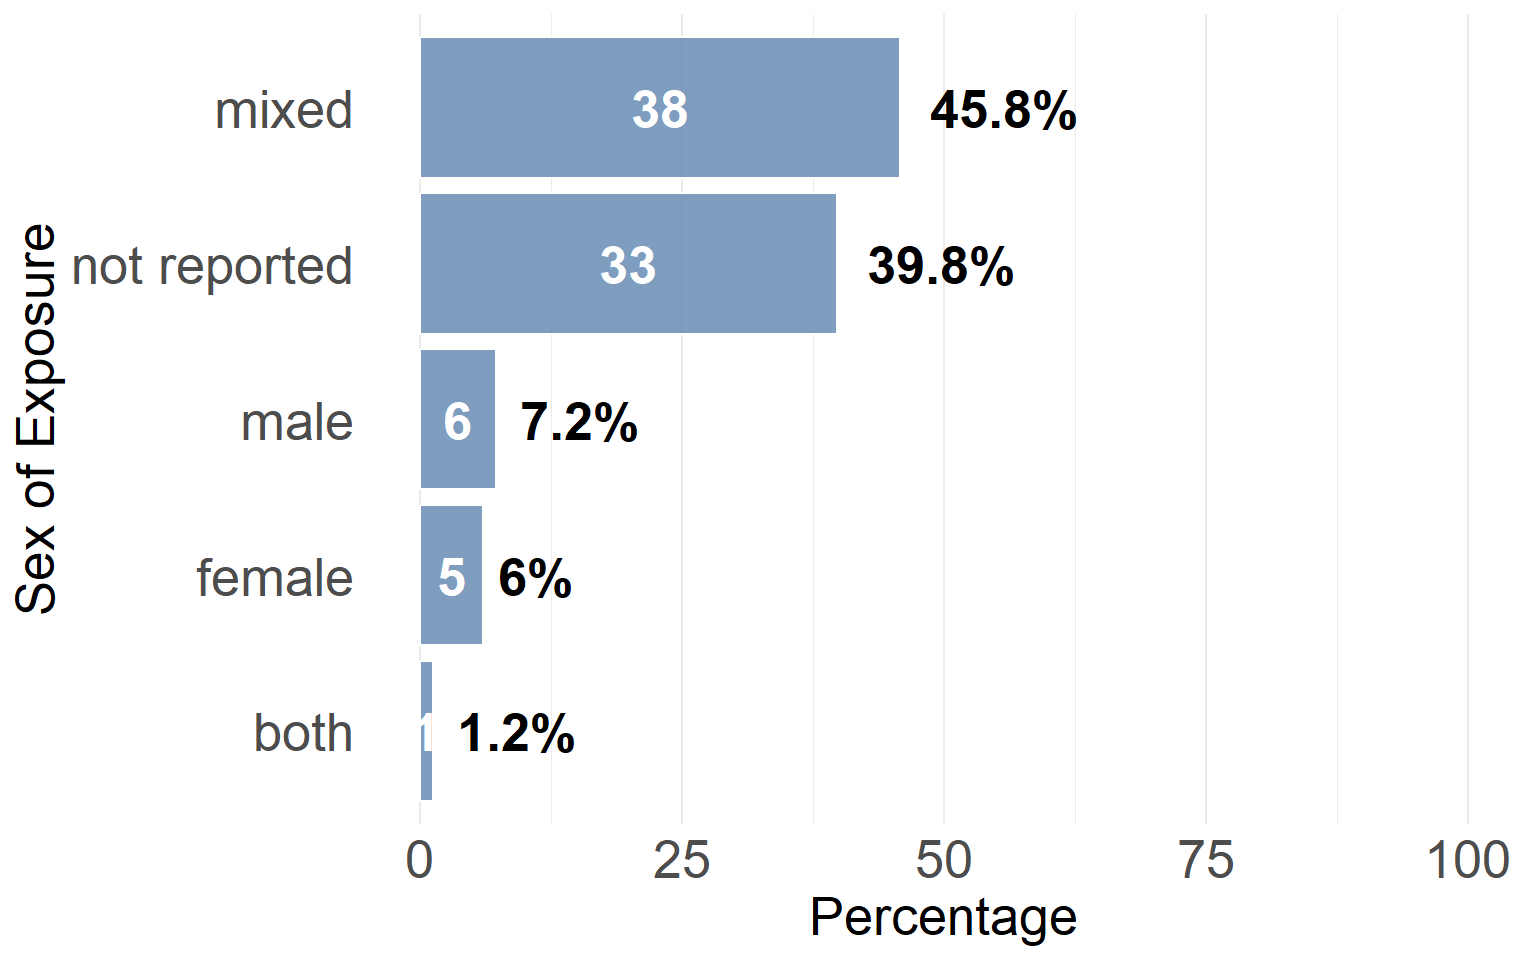
\includegraphics{zf_sm_code_files/figure-latex/unnamed-chunk-10-1.pdf}

\begin{Shaded}
\begin{Highlighting}[]
\FunctionTok{ggsave}\NormalTok{(}\FunctionTok{here}\NormalTok{(}\StringTok{"figures"}\NormalTok{, }\StringTok{"fig4\_pesticide\_dosage.pdf"}\NormalTok{), }\AttributeTok{width =} \DecValTok{16}\NormalTok{, }\AttributeTok{height =} \DecValTok{10}\NormalTok{, }\AttributeTok{units =} \StringTok{"cm"}\NormalTok{, }\AttributeTok{scale =} \DecValTok{2}\NormalTok{, }\AttributeTok{dpi =} \DecValTok{300}\NormalTok{, }\AttributeTok{device =}\NormalTok{ cairo\_pdf)}
\end{Highlighting}
\end{Shaded}

\hypertarget{figs4---comparison-of-lowest-and-highest-dosages-of-waterbourne-exposure-to-deltamethrin}{%
\subsection{figs4 - comparison of lowest and highest dosages of
waterbourne exposure to
deltamethrin}\label{figs4---comparison-of-lowest-and-highest-dosages-of-waterbourne-exposure-to-deltamethrin}}

\begin{Shaded}
\begin{Highlighting}[]
\CommentTok{\# Pivot the data set to a longer format, separating out the dosage type (lowest or highest) and value into separate columns}
\NormalTok{pdo\_waterbourne\_deltamethrin }\OtherTok{\textless{}{-}}\NormalTok{ pdo }\SpecialCharTok{\%\textgreater{}\%}
  \FunctionTok{pivot\_longer}\NormalTok{(}\AttributeTok{cols =} \FunctionTok{c}\NormalTok{(dosage\_lowest, dosage\_highest), }
               \AttributeTok{names\_to =} \StringTok{"dosage\_type"}\NormalTok{,}
               \AttributeTok{values\_to =} \StringTok{"dosage\_value"}\NormalTok{) }\SpecialCharTok{\%\textgreater{}\%} 
  
  \CommentTok{\# Filter for waterborne routes with consistent dosage units and only deltamethrin pesticide investigated}
  \FunctionTok{filter}\NormalTok{(route }\SpecialCharTok{==} \StringTok{"waterbourne"}\NormalTok{, dosage\_unit\_consistent }\SpecialCharTok{==} \StringTok{"ug/L"}\NormalTok{, pesticide\_investigated }\SpecialCharTok{==} \StringTok{"deltamethrin"}\NormalTok{) }\SpecialCharTok{\%\textgreater{}\%} 

  \CommentTok{\# Rename the dosage type column for better labeling in the plot}
  \FunctionTok{mutate}\NormalTok{(}\AttributeTok{dosage\_type =} \FunctionTok{if\_else}\NormalTok{(dosage\_type }\SpecialCharTok{==} \StringTok{"dosage\_lowest"}\NormalTok{, }\StringTok{"Lowest Dosage Exposed"}\NormalTok{, }\StringTok{"Highest Dosage Exposed"}\NormalTok{))}

\CommentTok{\# Create the plot with dosage type (i.e., lowest or highest dose) on the x{-}axis and dosage value on the y{-}axis}
\NormalTok{figs4 }\OtherTok{\textless{}{-}} \FunctionTok{ggplot}\NormalTok{(pdo\_waterbourne\_deltamethrin, }\FunctionTok{aes}\NormalTok{(}\AttributeTok{x =}\NormalTok{ dosage\_type, }\AttributeTok{y =} \FunctionTok{log}\NormalTok{(dosage\_value))) }\SpecialCharTok{+}
  
  \CommentTok{\# Add a violin plot }
  \FunctionTok{geom\_violin}\NormalTok{(}\AttributeTok{fill =} \StringTok{"\#5F85AE"}\NormalTok{, }\AttributeTok{alpha =} \FloatTok{0.2}\NormalTok{, }\AttributeTok{color =} \ConstantTok{NA}\NormalTok{, }\AttributeTok{trim =} \ConstantTok{FALSE}\NormalTok{) }\SpecialCharTok{+}
  
  \CommentTok{\# Add a boxplot }
  \FunctionTok{geom\_boxplot}\NormalTok{(}\AttributeTok{width =} \FloatTok{0.05}\NormalTok{, }\AttributeTok{fill =} \StringTok{"white"}\NormalTok{, }\AttributeTok{color =} \StringTok{"\#5F85AE"}\NormalTok{, }\AttributeTok{outlier.shape =} \ConstantTok{NA}\NormalTok{) }\SpecialCharTok{+}
  
  \CommentTok{\# Add jittered points}
  \FunctionTok{geom\_jitter}\NormalTok{(}\AttributeTok{width =} \FloatTok{0.1}\NormalTok{, }\AttributeTok{height =} \FloatTok{0.05}\NormalTok{, }\AttributeTok{color =} \StringTok{"\#5F85AE"}\NormalTok{, }\AttributeTok{alpha =} \FloatTok{0.5}\NormalTok{) }\SpecialCharTok{+}
  
  \CommentTok{\# Add axis and plot labels}
  \FunctionTok{labs}\NormalTok{(}\AttributeTok{title =} \StringTok{"Waterborne Exposures of Deltamethrin by Dosage in ug/L"}\NormalTok{, }\AttributeTok{x =} \StringTok{"Waterbourne exposure"}\NormalTok{, }\AttributeTok{y =} \StringTok{"log(Dosage (ug/L))"}\NormalTok{) }\SpecialCharTok{+}
  
  \CommentTok{\# Customize plot theme}
  \FunctionTok{theme\_minimal}\NormalTok{() }\SpecialCharTok{+}
  \FunctionTok{theme}\NormalTok{(}\AttributeTok{panel.grid.major.y =} \FunctionTok{element\_blank}\NormalTok{(),}
        \AttributeTok{axis.line.y =} \FunctionTok{element\_blank}\NormalTok{(),}
        \AttributeTok{axis.ticks.y =} \FunctionTok{element\_blank}\NormalTok{(),}
        \AttributeTok{axis.text.x =} \FunctionTok{element\_text}\NormalTok{(}\AttributeTok{size =} \DecValTok{15}\NormalTok{),}
        \AttributeTok{axis.text.y =} \FunctionTok{element\_text}\NormalTok{(}\AttributeTok{size =} \DecValTok{15}\NormalTok{, }\AttributeTok{hjust =} \DecValTok{1}\NormalTok{),}
        \AttributeTok{axis.title.x =} \FunctionTok{element\_text}\NormalTok{(}\AttributeTok{size =} \DecValTok{15}\NormalTok{),}
        \AttributeTok{axis.title.y =} \FunctionTok{element\_text}\NormalTok{(}\AttributeTok{size =} \DecValTok{15}\NormalTok{),}
        \AttributeTok{plot.title =} \FunctionTok{element\_blank}\NormalTok{())}

\CommentTok{\# figs4}
\end{Highlighting}
\end{Shaded}

\hypertarget{figs5---comparison-of-lowest-and-highest-dosages-of-waterbourne-exposure-to-rotenone}{%
\subsection{figs5 - comparison of lowest and highest dosages of
waterbourne exposure to
rotenone}\label{figs5---comparison-of-lowest-and-highest-dosages-of-waterbourne-exposure-to-rotenone}}

\begin{Shaded}
\begin{Highlighting}[]
\CommentTok{\# Pivot the data set to a longer format, separating out the dosage type (lowest or highest) and value into separate columns}
\NormalTok{pdo\_waterbourne\_rotenone }\OtherTok{\textless{}{-}}\NormalTok{ pdo }\SpecialCharTok{\%\textgreater{}\%}
  \FunctionTok{pivot\_longer}\NormalTok{(}\AttributeTok{cols =} \FunctionTok{c}\NormalTok{(dosage\_lowest, dosage\_highest), }
               \AttributeTok{names\_to =} \StringTok{"dosage\_type"}\NormalTok{,}
               \AttributeTok{values\_to =} \StringTok{"dosage\_value"}\NormalTok{) }\SpecialCharTok{\%\textgreater{}\%} 
  
  \CommentTok{\# Filter for waterborne routes with consistent dosage units and only rotenone pesticide investigated}
  \FunctionTok{filter}\NormalTok{(route }\SpecialCharTok{==} \StringTok{"waterbourne"}\NormalTok{, dosage\_unit\_consistent }\SpecialCharTok{==} \StringTok{"ug/L"}\NormalTok{, pesticide\_investigated }\SpecialCharTok{==} \StringTok{"rotenone"}\NormalTok{) }\SpecialCharTok{\%\textgreater{}\%} 
  
  \CommentTok{\# Rename the dosage type column for better labeling in the plot}
  \FunctionTok{mutate}\NormalTok{(}\AttributeTok{dosage\_type =} \FunctionTok{if\_else}\NormalTok{(dosage\_type }\SpecialCharTok{==} \StringTok{"dosage\_lowest"}\NormalTok{, }\StringTok{"Lowest Dosage Exposed"}\NormalTok{, }\StringTok{"Highest Dosage Exposed"}\NormalTok{))}

\CommentTok{\# Create the plot with dosage type (i.e., lowest or highest dose) on the x{-}axis and dosage value on the y{-}axis}
\NormalTok{figs5 }\OtherTok{\textless{}{-}} \FunctionTok{ggplot}\NormalTok{(pdo\_waterbourne\_rotenone, }\FunctionTok{aes}\NormalTok{(}\AttributeTok{x =}\NormalTok{ dosage\_type, }\AttributeTok{y =} \FunctionTok{log}\NormalTok{(dosage\_value))) }\SpecialCharTok{+}
  
  \CommentTok{\# Add a violin plot }
  \FunctionTok{geom\_violin}\NormalTok{(}\AttributeTok{fill =} \StringTok{"\#5F85AE"}\NormalTok{, }\AttributeTok{alpha =} \FloatTok{0.3}\NormalTok{, }\AttributeTok{trim =} \ConstantTok{FALSE}\NormalTok{, }\AttributeTok{color =} \ConstantTok{NA}\NormalTok{) }\SpecialCharTok{+}
  
  \CommentTok{\# Add a boxplot }
  \FunctionTok{geom\_boxplot}\NormalTok{(}\AttributeTok{width =} \FloatTok{0.05}\NormalTok{, }\AttributeTok{fill =} \StringTok{"white"}\NormalTok{, }\AttributeTok{color =} \StringTok{"\#5F85AE"}\NormalTok{, }\AttributeTok{outlier.shape =} \ConstantTok{NA}\NormalTok{) }\SpecialCharTok{+}
  
  \CommentTok{\# Add jittered points}
  \FunctionTok{geom\_jitter}\NormalTok{(}\AttributeTok{width =} \FloatTok{0.1}\NormalTok{, }\AttributeTok{height =} \FloatTok{0.05}\NormalTok{, }\AttributeTok{color =} \StringTok{"\#5F85AE"}\NormalTok{, }\AttributeTok{alpha =} \FloatTok{0.5}\NormalTok{) }\SpecialCharTok{+}
  
  \CommentTok{\# Add axis and plot labels}
  \FunctionTok{labs}\NormalTok{(}\AttributeTok{title =} \StringTok{"Waterborne Exposures of Rotenone by Dosage in ug/L"}\NormalTok{, }\AttributeTok{x =} \StringTok{"Waterbourne exposure"}\NormalTok{, }\AttributeTok{y =} \StringTok{"log(Dosage (ug/L))"}\NormalTok{) }\SpecialCharTok{+}
  
  \CommentTok{\# Customize plot theme}
  \FunctionTok{theme\_minimal}\NormalTok{() }\SpecialCharTok{+}
  \FunctionTok{theme}\NormalTok{(}\AttributeTok{panel.grid.major.y =} \FunctionTok{element\_blank}\NormalTok{(),}
        \AttributeTok{axis.line.y =} \FunctionTok{element\_blank}\NormalTok{(),}
        \AttributeTok{axis.ticks.y =} \FunctionTok{element\_blank}\NormalTok{(),}
        \AttributeTok{axis.text.x =} \FunctionTok{element\_text}\NormalTok{(}\AttributeTok{size =} \DecValTok{15}\NormalTok{),}
        \AttributeTok{axis.text.y =} \FunctionTok{element\_text}\NormalTok{(}\AttributeTok{size =} \DecValTok{15}\NormalTok{, }\AttributeTok{hjust =} \DecValTok{1}\NormalTok{),}
        \AttributeTok{axis.title.x =} \FunctionTok{element\_text}\NormalTok{(}\AttributeTok{size =} \DecValTok{15}\NormalTok{),}
        \AttributeTok{axis.title.y =} \FunctionTok{element\_text}\NormalTok{(}\AttributeTok{size =} \DecValTok{15}\NormalTok{),}
        \AttributeTok{plot.title =} \FunctionTok{element\_blank}\NormalTok{())}
\NormalTok{figs5}
\end{Highlighting}
\end{Shaded}

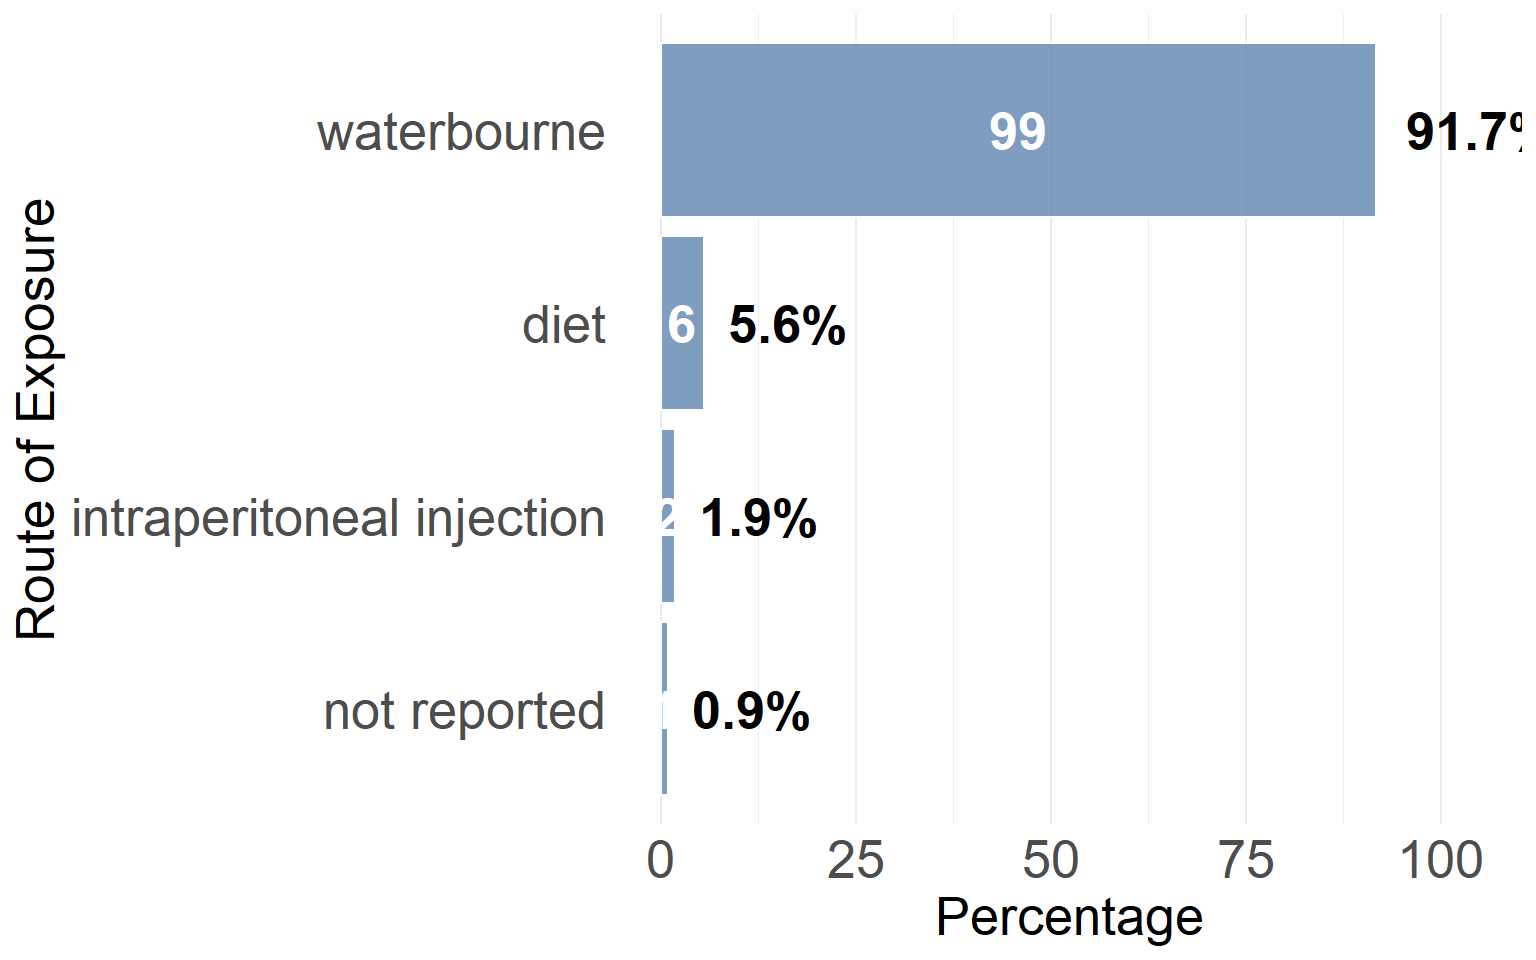
\includegraphics{zf_sm_code_files/figure-latex/unnamed-chunk-12-1.pdf}

\hypertarget{figs6---comparison-of-lowest-and-highest-dosages-of-waterbourne-exposure-atrazine}{%
\subsection{figs6 - comparison of lowest and highest dosages of
waterbourne exposure
atrazine}\label{figs6---comparison-of-lowest-and-highest-dosages-of-waterbourne-exposure-atrazine}}

\begin{Shaded}
\begin{Highlighting}[]
\CommentTok{\# Pivot the data set to a longer format, separating out the dosage type (lowest or highest) and value into separate columns}
\NormalTok{pdo\_waterbourne\_atrazine }\OtherTok{\textless{}{-}}\NormalTok{ pdo }\SpecialCharTok{\%\textgreater{}\%}
  \FunctionTok{pivot\_longer}\NormalTok{(}\AttributeTok{cols =} \FunctionTok{c}\NormalTok{(dosage\_lowest, dosage\_highest), }
               \AttributeTok{names\_to =} \StringTok{"dosage\_type"}\NormalTok{,}
               \AttributeTok{values\_to =} \StringTok{"dosage\_value"}\NormalTok{) }\SpecialCharTok{\%\textgreater{}\%} 

  \CommentTok{\# Filter for waterborne routes with consistent dosage units and only atrazine pesticide investigated}
  \FunctionTok{filter}\NormalTok{(route }\SpecialCharTok{==} \StringTok{"waterbourne"}\NormalTok{, dosage\_unit\_consistent }\SpecialCharTok{==} \StringTok{"ug/L"}\NormalTok{, pesticide\_investigated }\SpecialCharTok{==} \StringTok{"atrazine"}\NormalTok{) }\SpecialCharTok{\%\textgreater{}\%}  

  \CommentTok{\# Rename the dosage type column for better labeling in the plot}
  \FunctionTok{mutate}\NormalTok{(}\AttributeTok{dosage\_type =} \FunctionTok{if\_else}\NormalTok{(dosage\_type }\SpecialCharTok{==} \StringTok{"dosage\_lowest"}\NormalTok{, }\StringTok{"Lowest Dosage Exposed"}\NormalTok{, }\StringTok{"Highest Dosage Exposed"}\NormalTok{))}

\CommentTok{\# Create the plot with dosage type (i.e., lowest or highest dose) on the x{-}axis and dosage value on the y{-}axis}
\NormalTok{figs6 }\OtherTok{\textless{}{-}} \FunctionTok{ggplot}\NormalTok{(pdo\_waterbourne\_atrazine, }\FunctionTok{aes}\NormalTok{(}\AttributeTok{x =}\NormalTok{ dosage\_type, }\AttributeTok{y =} \FunctionTok{log}\NormalTok{(dosage\_value))) }\SpecialCharTok{+}

  \CommentTok{\# Add a violin plot }
  \FunctionTok{geom\_violin}\NormalTok{(}\AttributeTok{fill =} \StringTok{"\#5F85AE"}\NormalTok{, }\AttributeTok{alpha =} \FloatTok{0.3}\NormalTok{, }\AttributeTok{trim =} \ConstantTok{FALSE}\NormalTok{, }\AttributeTok{color =} \StringTok{"NA"}\NormalTok{) }\SpecialCharTok{+}

  \CommentTok{\# Add a boxplot }
  \FunctionTok{geom\_boxplot}\NormalTok{(}\AttributeTok{width =} \FloatTok{0.05}\NormalTok{, }\AttributeTok{fill =} \StringTok{"white"}\NormalTok{, }\AttributeTok{color =} \StringTok{"\#5F85AE"}\NormalTok{, }\AttributeTok{outlier.shape =} \ConstantTok{NA}\NormalTok{) }\SpecialCharTok{+}

  \CommentTok{\# Add jittered points}
  \FunctionTok{geom\_jitter}\NormalTok{(}\AttributeTok{width =} \FloatTok{0.1}\NormalTok{, }\AttributeTok{height =} \FloatTok{0.05}\NormalTok{, }\AttributeTok{color =} \StringTok{"\#5F85AE"}\NormalTok{, }\AttributeTok{alpha =} \FloatTok{0.5}\NormalTok{) }\SpecialCharTok{+}

  \CommentTok{\# Add axis and plot labels}
  \FunctionTok{labs}\NormalTok{(}\AttributeTok{title =} \StringTok{"Waterborne Exposures of Atrazine by Dosage in ug/L"}\NormalTok{, }\AttributeTok{x =} \StringTok{"Waterborne exposure"}\NormalTok{, }\AttributeTok{y =} \StringTok{"log(Dosage (ug/L))"}\NormalTok{)  }\SpecialCharTok{+}

  \CommentTok{\# Customize plot theme}
  \FunctionTok{theme\_minimal}\NormalTok{() }\SpecialCharTok{+}
  \FunctionTok{theme}\NormalTok{(}\AttributeTok{panel.grid.major.y =} \FunctionTok{element\_blank}\NormalTok{(),}
    \AttributeTok{axis.line.y =} \FunctionTok{element\_blank}\NormalTok{(),}
    \AttributeTok{axis.ticks.y =} \FunctionTok{element\_blank}\NormalTok{(),}
    \AttributeTok{axis.text.x =} \FunctionTok{element\_text}\NormalTok{(}\AttributeTok{size =} \DecValTok{15}\NormalTok{),}
    \AttributeTok{axis.text.y =} \FunctionTok{element\_text}\NormalTok{(}\AttributeTok{size =} \DecValTok{15}\NormalTok{, }\AttributeTok{hjust =} \DecValTok{1}\NormalTok{),}
    \AttributeTok{axis.title.x =} \FunctionTok{element\_text}\NormalTok{(}\AttributeTok{size =} \DecValTok{15}\NormalTok{),}
    \AttributeTok{axis.title.y =} \FunctionTok{element\_text}\NormalTok{(}\AttributeTok{size =} \DecValTok{15}\NormalTok{),}
    \AttributeTok{plot.title =} \FunctionTok{element\_blank}\NormalTok{())}


\NormalTok{figs6}
\end{Highlighting}
\end{Shaded}

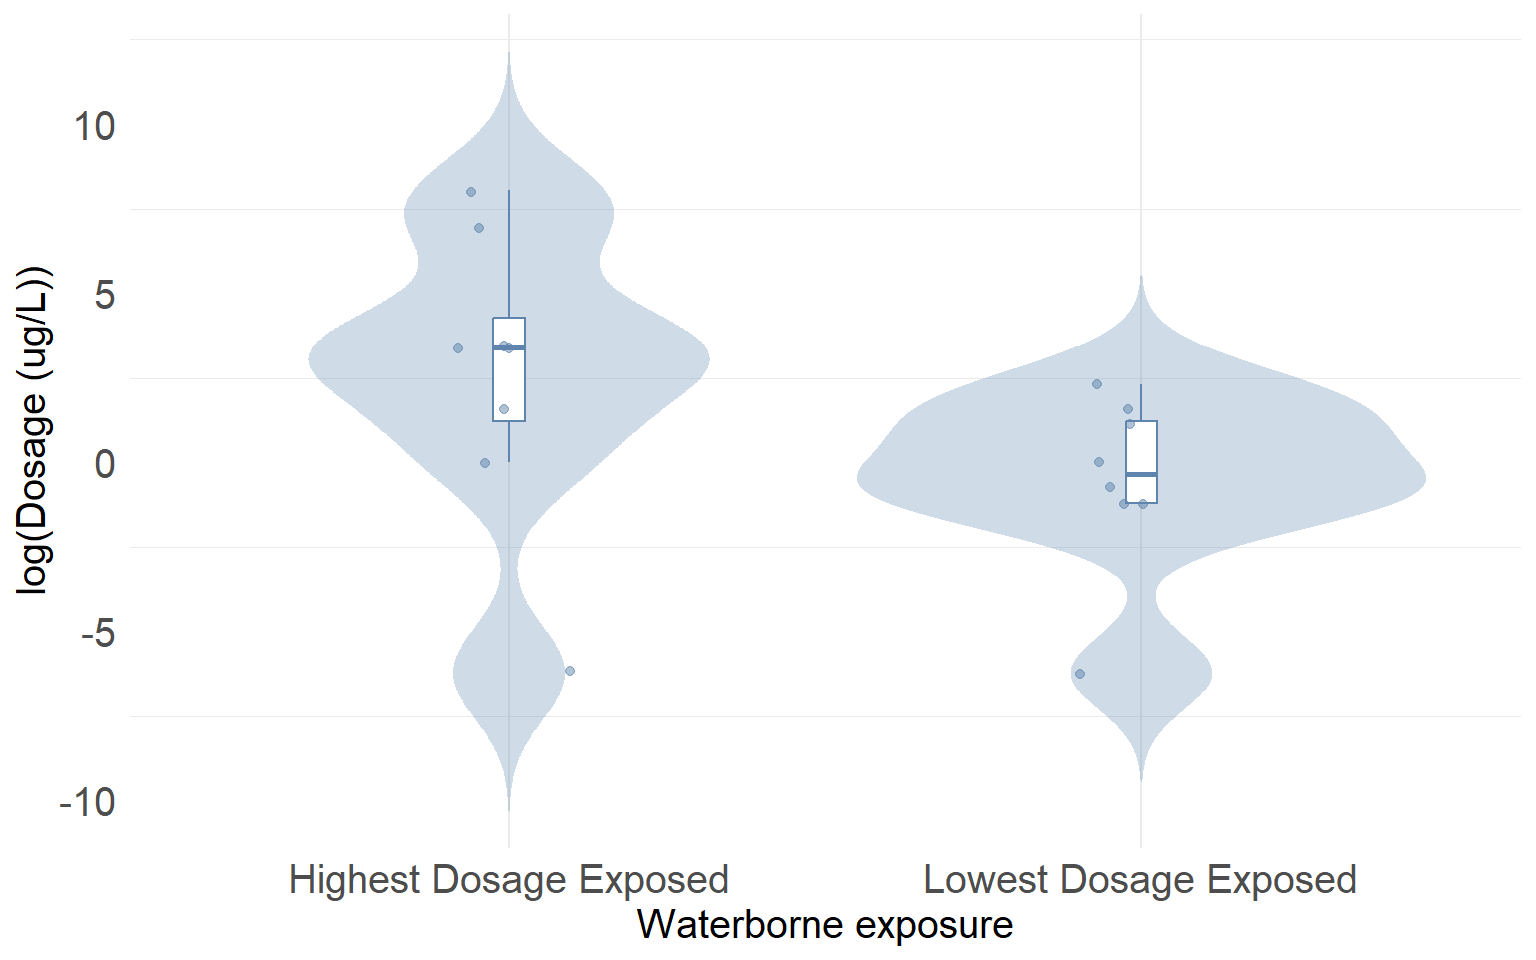
\includegraphics{zf_sm_code_files/figure-latex/unnamed-chunk-13-1.pdf}

\hypertarget{figs7---comparison-to-lowest-and-highest-dosages-of-waterbourne-exposure-to-glyphosate}{%
\subsection{figs7 - comparison to lowest and highest dosages of
waterbourne exposure to
glyphosate}\label{figs7---comparison-to-lowest-and-highest-dosages-of-waterbourne-exposure-to-glyphosate}}

\begin{Shaded}
\begin{Highlighting}[]
\CommentTok{\# Pivot the data set to a longer format, separating out the dosage type (lowest or highest) and value into separate columns}
\NormalTok{pdo\_waterbourne\_glyphosate }\OtherTok{\textless{}{-}}\NormalTok{ pdo }\SpecialCharTok{\%\textgreater{}\%}
  \FunctionTok{pivot\_longer}\NormalTok{(}\AttributeTok{cols =} \FunctionTok{c}\NormalTok{(dosage\_lowest, dosage\_highest), }
               \AttributeTok{names\_to =} \StringTok{"dosage\_type"}\NormalTok{,}
               \AttributeTok{values\_to =} \StringTok{"dosage\_value"}\NormalTok{) }\SpecialCharTok{\%\textgreater{}\%} 
  
  \CommentTok{\# Filter for waterborne routes with consistent dosage units and only glyphosate pesticide investigated}
  \FunctionTok{filter}\NormalTok{(route }\SpecialCharTok{==} \StringTok{"waterbourne"}\NormalTok{, dosage\_unit\_consistent }\SpecialCharTok{==} \StringTok{"ug/L"}\NormalTok{, pesticide\_investigated }\SpecialCharTok{==} \StringTok{"glyphosate"}\NormalTok{) }\SpecialCharTok{\%\textgreater{}\%}  
  
  \CommentTok{\# Rename the dosage type column for better labeling in the plot}
  \FunctionTok{mutate}\NormalTok{(}\AttributeTok{dosage\_type =} \FunctionTok{if\_else}\NormalTok{(dosage\_type }\SpecialCharTok{==} \StringTok{"dosage\_lowest"}\NormalTok{, }\StringTok{"Lowest Dosage Exposed"}\NormalTok{, }\StringTok{"Highest Dosage Exposed"}\NormalTok{))}


\CommentTok{\# Create the plot with dosage type (i.e., lowest or highest dose) on the x{-}axis and dosage value on the y{-}axis}
\NormalTok{figs7 }\OtherTok{\textless{}{-}} \FunctionTok{ggplot}\NormalTok{(pdo\_waterbourne\_glyphosate, }\FunctionTok{aes}\NormalTok{(}\AttributeTok{x =}\NormalTok{ dosage\_type, }\AttributeTok{y =} \FunctionTok{log}\NormalTok{(dosage\_value))) }\SpecialCharTok{+}
  
  \CommentTok{\# Add a violin plot}
 \FunctionTok{geom\_violin}\NormalTok{(}\AttributeTok{fill =} \StringTok{"\#5F85AE"}\NormalTok{, }\AttributeTok{alpha =} \FloatTok{0.3}\NormalTok{, }\AttributeTok{trim =} \ConstantTok{FALSE}\NormalTok{, }\AttributeTok{color =} \ConstantTok{NA}\NormalTok{) }\SpecialCharTok{+}
  
  \CommentTok{\# Add a boxplot}
  \FunctionTok{geom\_boxplot}\NormalTok{(}\AttributeTok{width =} \FloatTok{0.05}\NormalTok{, }\AttributeTok{fill =} \StringTok{"white"}\NormalTok{, }\AttributeTok{color =} \StringTok{"\#5F85AE"}\NormalTok{, }\AttributeTok{outlier.shape =} \ConstantTok{NA}\NormalTok{) }\SpecialCharTok{+}
  
  \CommentTok{\# Add jittered points}
  \FunctionTok{geom\_jitter}\NormalTok{(}\AttributeTok{width =} \FloatTok{0.1}\NormalTok{, }\AttributeTok{height =} \FloatTok{0.05}\NormalTok{, }\AttributeTok{color =} \StringTok{"\#5F85AE"}\NormalTok{, }\AttributeTok{alpha =} \FloatTok{0.5}\NormalTok{) }\SpecialCharTok{+}
  
  \CommentTok{\# Add axis and plot labels}
  \FunctionTok{labs}\NormalTok{(}\AttributeTok{title =} \StringTok{"Waterborne Exposures of Glyphosate by Dosage in ug/L"}\NormalTok{, }\AttributeTok{x =} \StringTok{"Waterbourne exposure"}\NormalTok{, }\AttributeTok{y =} \StringTok{"log(Dosage (ug/L))"}\NormalTok{)  }\SpecialCharTok{+}
  
  \CommentTok{\# Customize plot theme}
  \FunctionTok{theme\_minimal}\NormalTok{() }\SpecialCharTok{+}
  \FunctionTok{theme}\NormalTok{(}\AttributeTok{panel.grid.major.y =} \FunctionTok{element\_blank}\NormalTok{(),}
    \AttributeTok{axis.line.y =} \FunctionTok{element\_blank}\NormalTok{(),}
    \AttributeTok{axis.ticks.y =} \FunctionTok{element\_blank}\NormalTok{(),}
    \AttributeTok{axis.text.x =} \FunctionTok{element\_text}\NormalTok{(}\AttributeTok{size =} \DecValTok{15}\NormalTok{),}
    \AttributeTok{axis.text.y =} \FunctionTok{element\_text}\NormalTok{(}\AttributeTok{size =} \DecValTok{15}\NormalTok{, }\AttributeTok{hjust =} \DecValTok{1}\NormalTok{),}
    \AttributeTok{axis.title.x =} \FunctionTok{element\_text}\NormalTok{(}\AttributeTok{size =} \DecValTok{15}\NormalTok{),}
    \AttributeTok{axis.title.y =} \FunctionTok{element\_text}\NormalTok{(}\AttributeTok{size =} \DecValTok{15}\NormalTok{),}
    \AttributeTok{plot.title =} \FunctionTok{element\_blank}\NormalTok{())}
\NormalTok{figs7}
\end{Highlighting}
\end{Shaded}

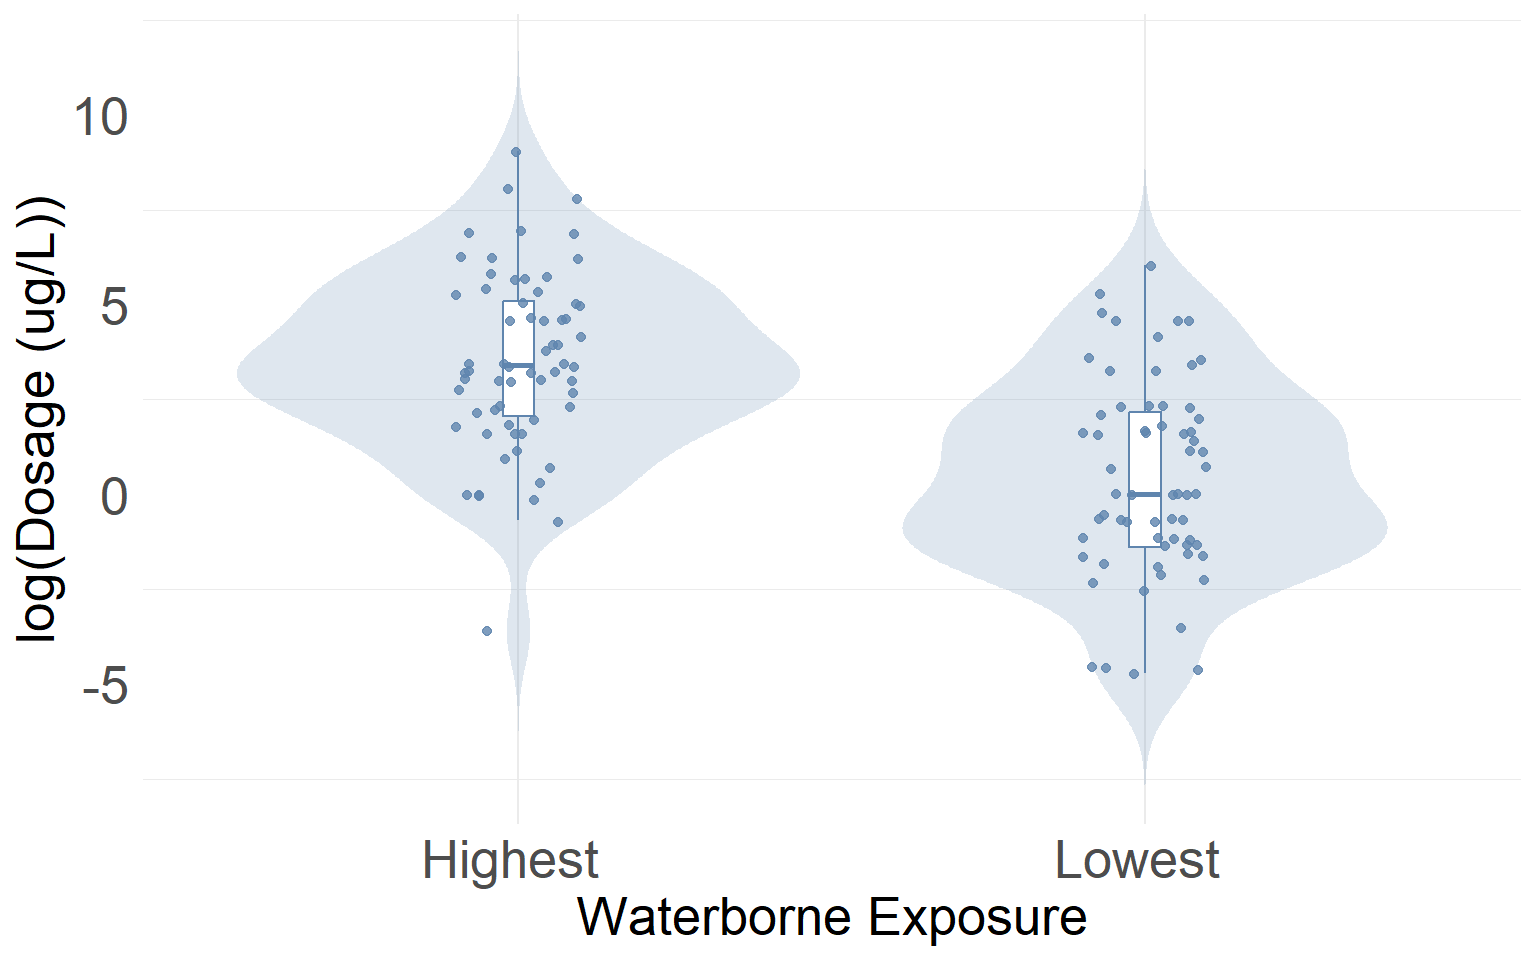
\includegraphics{zf_sm_code_files/figure-latex/unnamed-chunk-14-1.pdf}

\hypertarget{figs8---comparison-to-lowest-and-highest-dosages-of-waterbourne-exposure-to-chlopyrifo}{%
\subsection{figs8 - comparison to lowest and highest dosages of
waterbourne exposure to
chlopyrifo}\label{figs8---comparison-to-lowest-and-highest-dosages-of-waterbourne-exposure-to-chlopyrifo}}

\begin{Shaded}
\begin{Highlighting}[]
\CommentTok{\# Pivot the data set to a longer format, separating out the dosage type (lowest or highest) and value into separate columns}
\NormalTok{pdo\_waterbourne\_chloropyrifo }\OtherTok{\textless{}{-}}\NormalTok{ pdo }\SpecialCharTok{\%\textgreater{}\%}
  \FunctionTok{pivot\_longer}\NormalTok{(}\AttributeTok{cols =} \FunctionTok{c}\NormalTok{(dosage\_lowest, dosage\_highest), }
               \AttributeTok{names\_to =} \StringTok{"dosage\_type"}\NormalTok{,}
               \AttributeTok{values\_to =} \StringTok{"dosage\_value"}\NormalTok{) }\SpecialCharTok{\%\textgreater{}\%} 
  
  \CommentTok{\# Filter for waterborne routes with consistent dosage units and only glyphosate pesticide investigated}
  \FunctionTok{filter}\NormalTok{(route }\SpecialCharTok{==} \StringTok{"waterbourne"}\NormalTok{, dosage\_unit\_consistent }\SpecialCharTok{==} \StringTok{"ug/L"}\NormalTok{, pesticide\_investigated }\SpecialCharTok{==} \StringTok{"chloropyrifo"}\NormalTok{) }\SpecialCharTok{\%\textgreater{}\%}  
  
  \CommentTok{\# Rename the dosage type column for better labeling in the plot}
  \FunctionTok{mutate}\NormalTok{(}\AttributeTok{dosage\_type =} \FunctionTok{if\_else}\NormalTok{(dosage\_type }\SpecialCharTok{==} \StringTok{"dosage\_lowest"}\NormalTok{, }\StringTok{"Lowest Dosage Exposed"}\NormalTok{, }\StringTok{"Highest Dosage Exposed"}\NormalTok{))}

\CommentTok{\# Create the plot with dosage type (i.e., lowest or highest dose) on the x{-}axis and dosage value on the y{-}axis}
\NormalTok{figs8 }\OtherTok{\textless{}{-}} \FunctionTok{ggplot}\NormalTok{(pdo\_waterbourne\_chloropyrifo, }\FunctionTok{aes}\NormalTok{(}\AttributeTok{x =}\NormalTok{ dosage\_type, }\AttributeTok{y =} \FunctionTok{log}\NormalTok{(dosage\_value))) }\SpecialCharTok{+}
  
  \CommentTok{\# Add a violin plot}
  \FunctionTok{geom\_violin}\NormalTok{(}\AttributeTok{fill =} \StringTok{"\#5F85AE"}\NormalTok{, }\AttributeTok{alpha =} \FloatTok{0.3}\NormalTok{, }\AttributeTok{trim =} \ConstantTok{FALSE}\NormalTok{, }\AttributeTok{color =} \ConstantTok{NA}\NormalTok{) }\SpecialCharTok{+}
  
  \CommentTok{\# Add a boxplot}
  \FunctionTok{geom\_boxplot}\NormalTok{(}\AttributeTok{width =} \FloatTok{0.05}\NormalTok{, }\AttributeTok{fill =} \StringTok{"white"}\NormalTok{, }\AttributeTok{color =} \StringTok{"\#5F85AE"}\NormalTok{, }\AttributeTok{outlier.shape =} \ConstantTok{NA}\NormalTok{) }\SpecialCharTok{+}
  
  \CommentTok{\# Add jittered points}
  \FunctionTok{geom\_jitter}\NormalTok{(}\AttributeTok{width =} \FloatTok{0.1}\NormalTok{, }\AttributeTok{height =} \FloatTok{0.05}\NormalTok{, }\AttributeTok{color =} \StringTok{"\#5F85AE"}\NormalTok{, }\AttributeTok{alpha =} \FloatTok{0.5}\NormalTok{) }\SpecialCharTok{+}

  \CommentTok{\# Add axis and plot labels}
  \FunctionTok{labs}\NormalTok{(}\AttributeTok{title =} \StringTok{"Waterborne Exposures of Chloropyrifos by Dosage in ug/L"}\NormalTok{, }\AttributeTok{x =} \StringTok{"Waterbourne exposure"}\NormalTok{, }\AttributeTok{y =} \StringTok{"log(Dosage (ug/L))"}\NormalTok{)  }\SpecialCharTok{+}
  
  \CommentTok{\# Customize plot theme}
  \FunctionTok{theme\_minimal}\NormalTok{() }\SpecialCharTok{+}
  \FunctionTok{theme}\NormalTok{(}\AttributeTok{panel.grid.major.y =} \FunctionTok{element\_blank}\NormalTok{(),}
    \AttributeTok{axis.line.y =} \FunctionTok{element\_blank}\NormalTok{(),}
    \AttributeTok{axis.ticks.y =} \FunctionTok{element\_blank}\NormalTok{(),}
    \AttributeTok{axis.text.x =} \FunctionTok{element\_text}\NormalTok{(}\AttributeTok{size =} \DecValTok{15}\NormalTok{),}
    \AttributeTok{axis.text.y =} \FunctionTok{element\_text}\NormalTok{(}\AttributeTok{size =} \DecValTok{15}\NormalTok{, }\AttributeTok{hjust =} \DecValTok{1}\NormalTok{),}
    \AttributeTok{axis.title.x =} \FunctionTok{element\_text}\NormalTok{(}\AttributeTok{size =} \DecValTok{15}\NormalTok{),}
    \AttributeTok{axis.title.y =} \FunctionTok{element\_text}\NormalTok{(}\AttributeTok{size =} \DecValTok{15}\NormalTok{),}
    \AttributeTok{plot.title =} \FunctionTok{element\_blank}\NormalTok{())}
\NormalTok{figs8}
\end{Highlighting}
\end{Shaded}

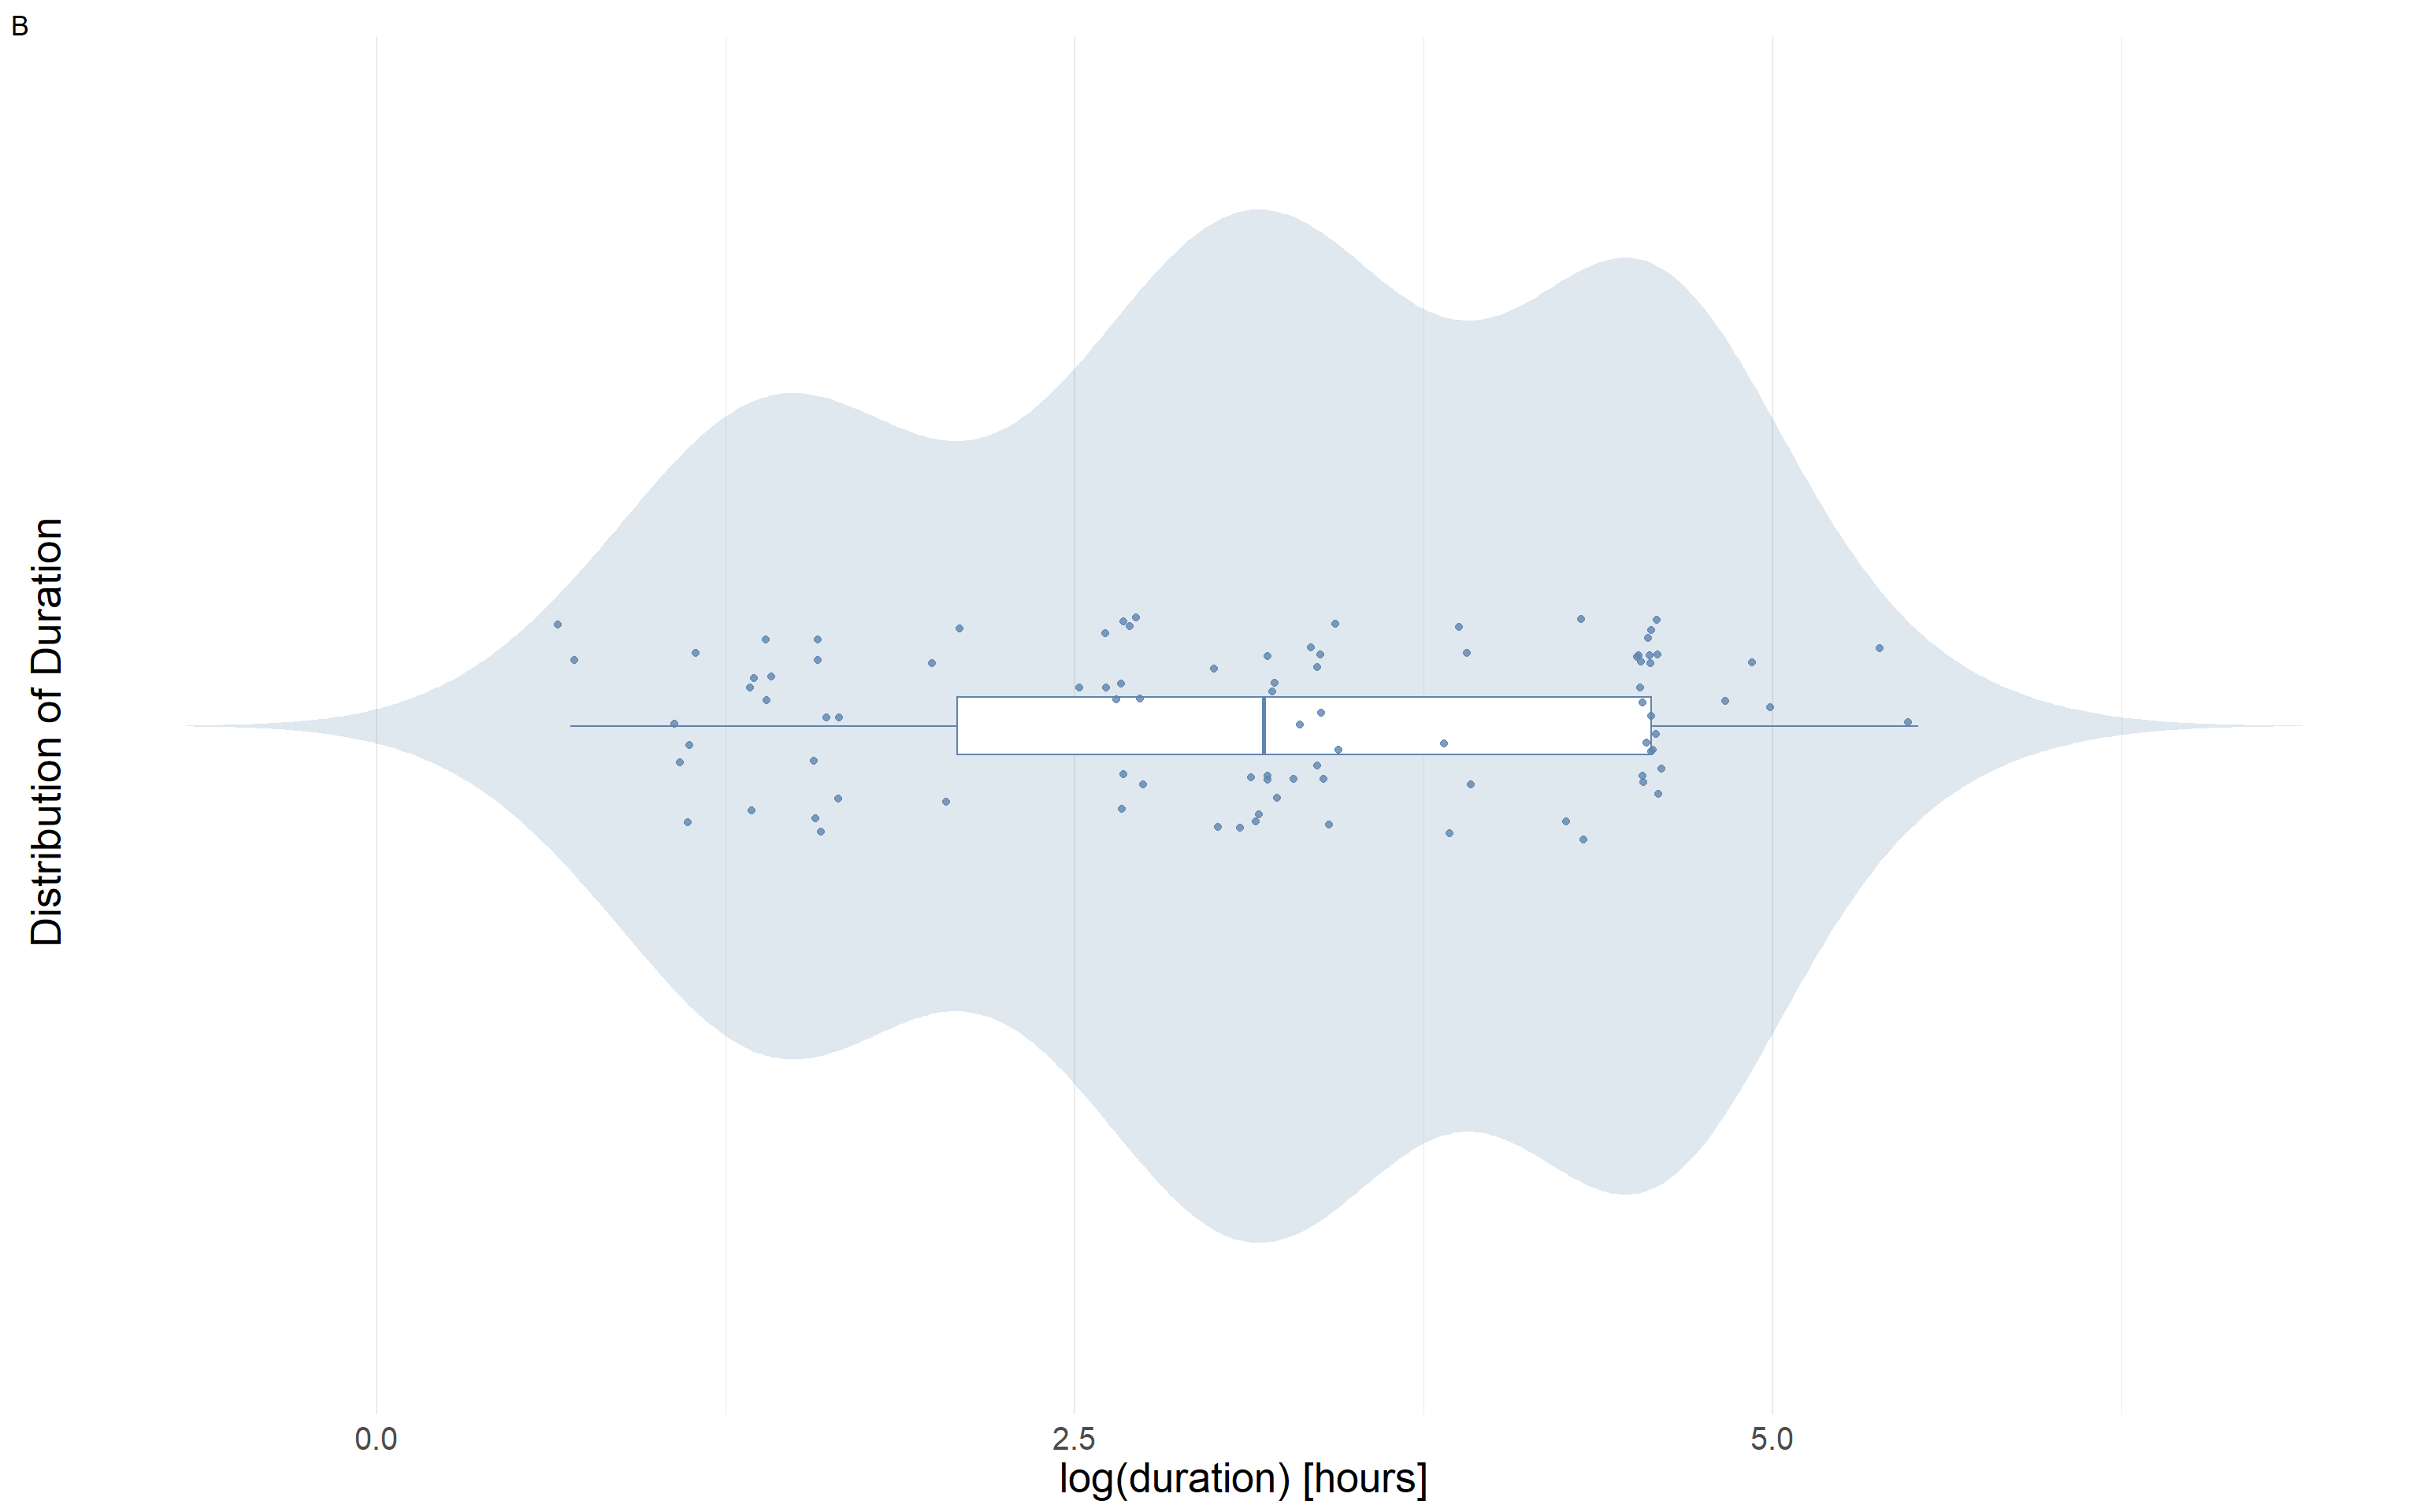
\includegraphics{zf_sm_code_files/figure-latex/unnamed-chunk-15-1.pdf}

\hypertarget{figx---durations-of-waterbourne-exposure}{%
\subsection{figx - durations of waterbourne
exposure}\label{figx---durations-of-waterbourne-exposure}}

\begin{Shaded}
\begin{Highlighting}[]
\NormalTok{pdo }\OtherTok{\textless{}{-}}\NormalTok{ pdo }\SpecialCharTok{\%\textgreater{}\%} 
  \FunctionTok{filter}\NormalTok{(}\SpecialCharTok{!}\FunctionTok{is.na}\NormalTok{(duration)) }\SpecialCharTok{\%\textgreater{}\%}
  \CommentTok{\# Convert duration to numeric and duration\_unit to character }
  \FunctionTok{mutate}\NormalTok{(}\AttributeTok{duration =} \FunctionTok{as.numeric}\NormalTok{(duration),}
         \AttributeTok{duration\_unit =} \FunctionTok{as.character}\NormalTok{(duration\_unit),}
         
  \CommentTok{\# Standardize duration\_unit\_consistent based on dosage\_unit }
  \AttributeTok{duration\_unit\_consistent =} \FunctionTok{case\_when}\NormalTok{(}
\NormalTok{          duration\_unit }\SpecialCharTok{==} \StringTok{"minutes"} \SpecialCharTok{\textasciitilde{}} \StringTok{"hours"}\NormalTok{,}
        
\NormalTok{          duration\_unit }\SpecialCharTok{==} \StringTok{"days"} \SpecialCharTok{\textasciitilde{}} \StringTok{"hours"}\NormalTok{,}
\NormalTok{          duration\_unit }\SpecialCharTok{==} \StringTok{"weeks"} \SpecialCharTok{\textasciitilde{}} \StringTok{"hours"}\NormalTok{,}
           \ConstantTok{TRUE} \SpecialCharTok{\textasciitilde{}}\NormalTok{ duration\_unit),}
  
  \CommentTok{\# Convert duration to hours based on duration\_unit}
  
  \AttributeTok{duration\_convert =} \FunctionTok{case\_when}\NormalTok{(}
\NormalTok{    duration\_unit }\SpecialCharTok{==} \StringTok{"minutes"} \SpecialCharTok{\textasciitilde{}}\NormalTok{ duration}\SpecialCharTok{*} \DecValTok{60}\NormalTok{,}
\NormalTok{    duration\_unit }\SpecialCharTok{==} \StringTok{"days"} \SpecialCharTok{\textasciitilde{}}\NormalTok{ duration}\SpecialCharTok{/}\DecValTok{24}\NormalTok{, }
\NormalTok{    duration\_unit }\SpecialCharTok{==} \StringTok{"weeks"} \SpecialCharTok{\textasciitilde{}}\NormalTok{ duration}\SpecialCharTok{/}\DecValTok{168}\NormalTok{,}
    \ConstantTok{TRUE} \SpecialCharTok{\textasciitilde{}}\NormalTok{ duration)) }\SpecialCharTok{\%\textgreater{}\%} 
  \FunctionTok{filter}\NormalTok{(route }\SpecialCharTok{==} \StringTok{"waterbourne"}\NormalTok{)}
\end{Highlighting}
\end{Shaded}

\begin{verbatim}
## Warning: There was 1 warning in `mutate()`.
## i In argument: `duration = as.numeric(duration)`.
## Caused by warning:
## ! NAs introduced by coercion
\end{verbatim}

\begin{Shaded}
\begin{Highlighting}[]
\NormalTok{figx }\OtherTok{\textless{}{-}} \FunctionTok{ggplot}\NormalTok{(pdo, }\FunctionTok{aes}\NormalTok{(}\AttributeTok{x =}\NormalTok{ route , }\AttributeTok{y =} \FunctionTok{log}\NormalTok{(duration))) }\SpecialCharTok{+} 
    \CommentTok{\# Add a violin plot }
  \FunctionTok{geom\_violin}\NormalTok{(}\AttributeTok{fill =} \StringTok{"\#5F85AE"}\NormalTok{, }\AttributeTok{alpha =}\FloatTok{0.2}\NormalTok{, }\AttributeTok{color =} \ConstantTok{NA}\NormalTok{, }\AttributeTok{trim =} \ConstantTok{FALSE}\NormalTok{) }\SpecialCharTok{+}

  \CommentTok{\# Add a boxplot }
  \FunctionTok{geom\_boxplot}\NormalTok{(}\AttributeTok{width =} \FloatTok{0.05}\NormalTok{, }\AttributeTok{fill =} \StringTok{"white"}\NormalTok{, }\AttributeTok{color =} \StringTok{"\#5F85AE"}\NormalTok{, }\AttributeTok{outlier.shape =} \ConstantTok{NA}\NormalTok{) }\SpecialCharTok{+}

  \CommentTok{\# Add jittered points }
  \FunctionTok{geom\_jitter}\NormalTok{(}\AttributeTok{width =} \FloatTok{0.1}\NormalTok{, }\AttributeTok{height =} \FloatTok{0.05}\NormalTok{, }\AttributeTok{color =} \StringTok{"\#5F85AE"}\NormalTok{, }\AttributeTok{alpha =} \FloatTok{0.8}\NormalTok{) }\SpecialCharTok{+}

  
  \CommentTok{\# Add axis and plot labels}
  \FunctionTok{labs}\NormalTok{(}\AttributeTok{x =} \StringTok{"Route "}\NormalTok{, }\AttributeTok{y =} \StringTok{"log(duration (hours))"}\NormalTok{) }\SpecialCharTok{+}
  
  \CommentTok{\# Customize plot theme}
  \FunctionTok{theme\_minimal}\NormalTok{() }\SpecialCharTok{+}
  \FunctionTok{theme}\NormalTok{(}\AttributeTok{panel.grid.major.y =} \FunctionTok{element\_blank}\NormalTok{(),}
    \AttributeTok{axis.line.y =} \FunctionTok{element\_blank}\NormalTok{(),}
    \AttributeTok{axis.ticks.y =} \FunctionTok{element\_blank}\NormalTok{(),}
    \AttributeTok{axis.text.x =} \FunctionTok{element\_text}\NormalTok{(}\AttributeTok{size =} \DecValTok{15}\NormalTok{),}
    \AttributeTok{axis.text.y =} \FunctionTok{element\_text}\NormalTok{(}\AttributeTok{size =} \DecValTok{15}\NormalTok{),}
    \AttributeTok{axis.title.x =} \FunctionTok{element\_text}\NormalTok{(}\AttributeTok{size =} \DecValTok{15}\NormalTok{),}
    \AttributeTok{axis.title.y =} \FunctionTok{element\_text}\NormalTok{(}\AttributeTok{size =} \DecValTok{15}\NormalTok{),}
    \AttributeTok{plot.title =} \FunctionTok{element\_blank}\NormalTok{())}

\NormalTok{figx}
\end{Highlighting}
\end{Shaded}

\begin{verbatim}
## Warning: Removed 7 rows containing non-finite values (`stat_ydensity()`).
\end{verbatim}

\begin{verbatim}
## Warning: Removed 7 rows containing non-finite values (`stat_boxplot()`).
\end{verbatim}

\begin{verbatim}
## Warning: Removed 7 rows containing missing values (`geom_point()`).
\end{verbatim}

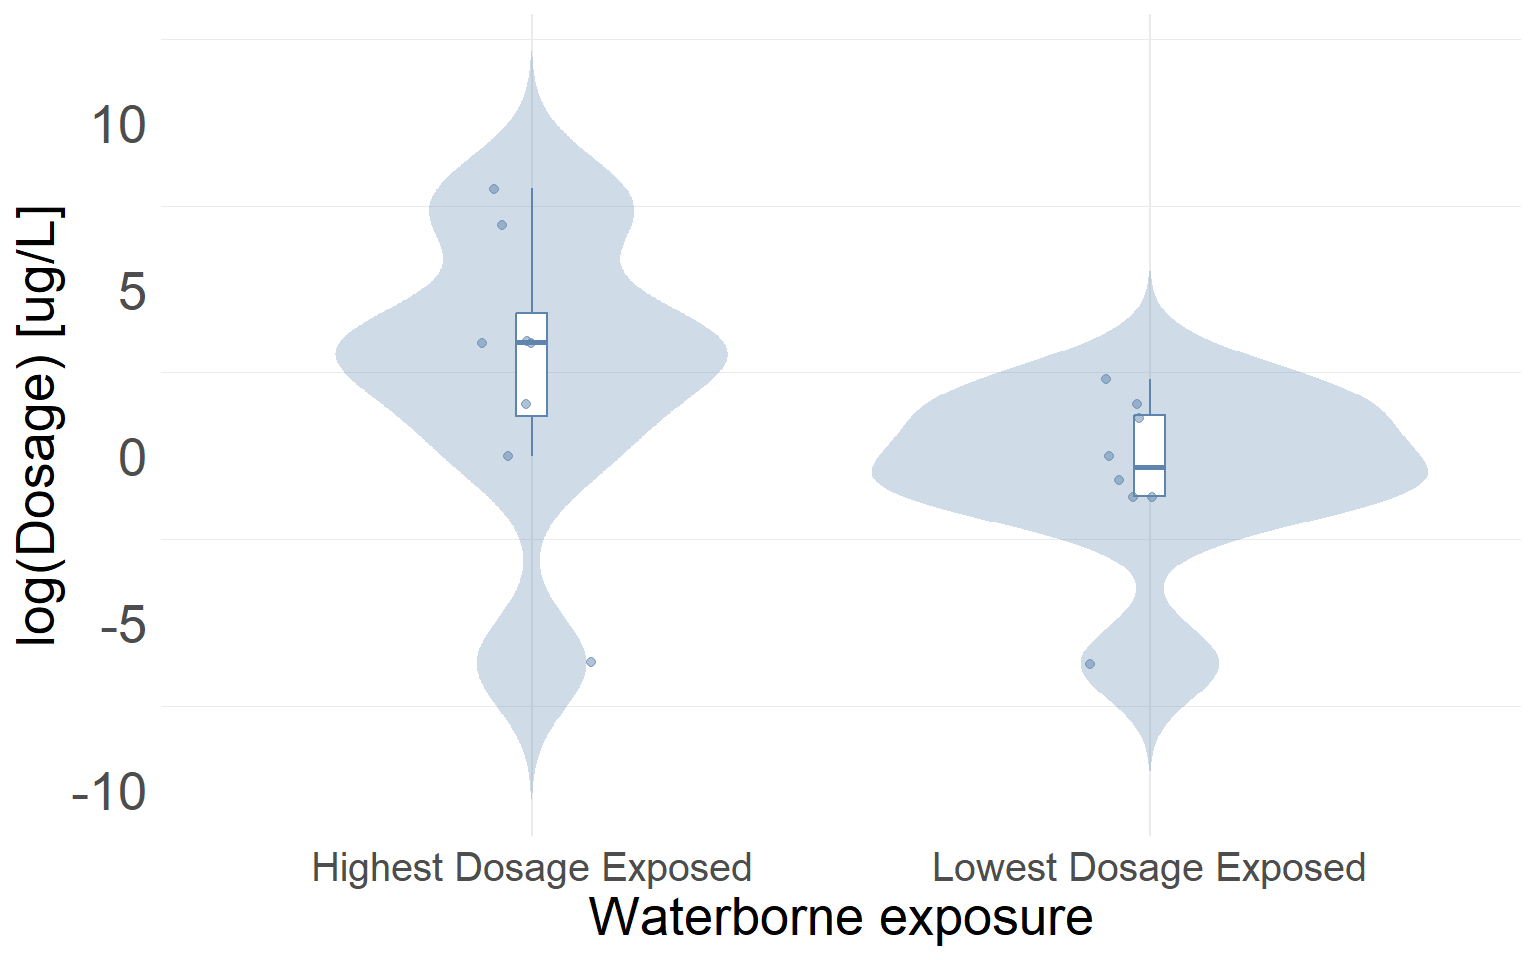
\includegraphics{zf_sm_code_files/figure-latex/unnamed-chunk-16-1.pdf}

\hypertarget{figs9---total-lifestage-of-exposure-completed-as-a-percentage}{%
\subsection{figs9 - total lifestage of exposure completed as a
percentage}\label{figs9---total-lifestage-of-exposure-completed-as-a-percentage}}

\begin{Shaded}
\begin{Highlighting}[]
\CommentTok{\# Calculate total count for each category}
\NormalTok{total\_count\_lse }\OtherTok{\textless{}{-}}\NormalTok{ sd }\SpecialCharTok{\%\textgreater{}\%} \FunctionTok{count}\NormalTok{(life\_stage\_exposure)}

\CommentTok{\# Calculate proportion and percentage for each category}
\NormalTok{life\_stage\_pct }\OtherTok{\textless{}{-}}\NormalTok{ sd }\SpecialCharTok{\%\textgreater{}\%}
    \FunctionTok{separate\_rows}\NormalTok{(life\_stage\_exposure, }\AttributeTok{sep =} \StringTok{",}\SpecialCharTok{\textbackslash{}\textbackslash{}}\StringTok{s*"}\NormalTok{) }\SpecialCharTok{\%\textgreater{}\%} 
  \FunctionTok{count}\NormalTok{(life\_stage\_exposure) }\SpecialCharTok{\%\textgreater{}\%}
  \FunctionTok{mutate}\NormalTok{(}\AttributeTok{proportion =}\NormalTok{ n}\SpecialCharTok{/}\FunctionTok{sum}\NormalTok{(total\_count\_lse}\SpecialCharTok{$}\NormalTok{n),}
         \AttributeTok{percentage =}\NormalTok{ proportion}\SpecialCharTok{*}\DecValTok{100}\NormalTok{)}

 \CommentTok{\# Create a bar chart with the count on the x{-}axis and life stage of exposure  on the y{-}axis}
\NormalTok{figs9 }\OtherTok{\textless{}{-}} \FunctionTok{ggplot}\NormalTok{(life\_stage\_pct, }\FunctionTok{aes}\NormalTok{(}\AttributeTok{x =} \FunctionTok{reorder}\NormalTok{(life\_stage\_exposure, percentage), }\AttributeTok{y =}\NormalTok{ percentage)) }\SpecialCharTok{+}
  
  \CommentTok{\# Customize the appearance of the bars }
   \FunctionTok{geom\_bar}\NormalTok{(}\AttributeTok{stat =} \StringTok{"identity"}\NormalTok{, }\AttributeTok{fill =} \StringTok{"\#5F85AE"}\NormalTok{, }\AttributeTok{color =} \StringTok{"white"}\NormalTok{, }\AttributeTok{alpha =} \FloatTok{0.8}\NormalTok{, }\AttributeTok{position =} \FunctionTok{position\_dodge}\NormalTok{(}\FloatTok{0.9}\NormalTok{)) }\SpecialCharTok{+}
  
  \CommentTok{\# Add labels to the bars for percentage }
  \FunctionTok{geom\_text}\NormalTok{(}\FunctionTok{aes}\NormalTok{(}\AttributeTok{label =} \FunctionTok{paste0}\NormalTok{(}\FunctionTok{round}\NormalTok{(percentage, }\DecValTok{1}\NormalTok{), }\StringTok{"\%"}\NormalTok{)), }\AttributeTok{hjust =} \SpecialCharTok{{-}}\FloatTok{0.2}\NormalTok{, }\AttributeTok{vjust =} \FloatTok{0.5}\NormalTok{, }\AttributeTok{size =} \DecValTok{5}\NormalTok{, }\AttributeTok{fontface =} \StringTok{"bold"}\NormalTok{) }\SpecialCharTok{+}
  
   \CommentTok{\# Add absolute count to bars}
  \FunctionTok{geom\_text}\NormalTok{(}\FunctionTok{aes}\NormalTok{(}\AttributeTok{label =}\NormalTok{ n), }\AttributeTok{position =} \FunctionTok{position\_stack}\NormalTok{(}\AttributeTok{vjust =} \FloatTok{0.5}\NormalTok{), }\AttributeTok{color =} \StringTok{"white"}\NormalTok{, }\AttributeTok{fontface =} \StringTok{"bold"}\NormalTok{, }\AttributeTok{size =} \DecValTok{5}\NormalTok{) }\SpecialCharTok{+}
  
  \CommentTok{\# Add axis and plot labels }
  \FunctionTok{labs}\NormalTok{( }\AttributeTok{x =} \StringTok{"Life Stage of Exposure"}\NormalTok{, }\AttributeTok{y =} \StringTok{"Percentage"}\NormalTok{, }\AttributeTok{fontsize =} \DecValTok{14}\NormalTok{) }\SpecialCharTok{+}
  
  \CommentTok{\# Customize the plot theme }
  \FunctionTok{theme\_minimal}\NormalTok{() }\SpecialCharTok{+}
  \FunctionTok{theme}\NormalTok{(}\AttributeTok{panel.grid.major.y =} \FunctionTok{element\_blank}\NormalTok{(),}
    \AttributeTok{axis.line.y =} \FunctionTok{element\_blank}\NormalTok{(),}
    \AttributeTok{axis.ticks.y =} \FunctionTok{element\_blank}\NormalTok{(),}
    \AttributeTok{axis.text.x =} \FunctionTok{element\_text}\NormalTok{(}\AttributeTok{size =} \DecValTok{15}\NormalTok{),}
    \AttributeTok{axis.text.y =} \FunctionTok{element\_text}\NormalTok{(}\AttributeTok{size =} \DecValTok{15}\NormalTok{, }\AttributeTok{hjust =} \DecValTok{1}\NormalTok{),}
    \AttributeTok{axis.title.x =} \FunctionTok{element\_text}\NormalTok{(}\AttributeTok{size =} \DecValTok{15}\NormalTok{),}
    \AttributeTok{axis.title.y =} \FunctionTok{element\_text}\NormalTok{(}\AttributeTok{size =} \DecValTok{15}\NormalTok{),}
    \AttributeTok{plot.title =} \FunctionTok{element\_blank}\NormalTok{()) }\SpecialCharTok{+}
  \FunctionTok{coord\_flip}\NormalTok{() }\SpecialCharTok{+} 
  \FunctionTok{ylim}\NormalTok{(}\DecValTok{0}\NormalTok{, }\DecValTok{100}\NormalTok{)}

\NormalTok{figs9}
\end{Highlighting}
\end{Shaded}

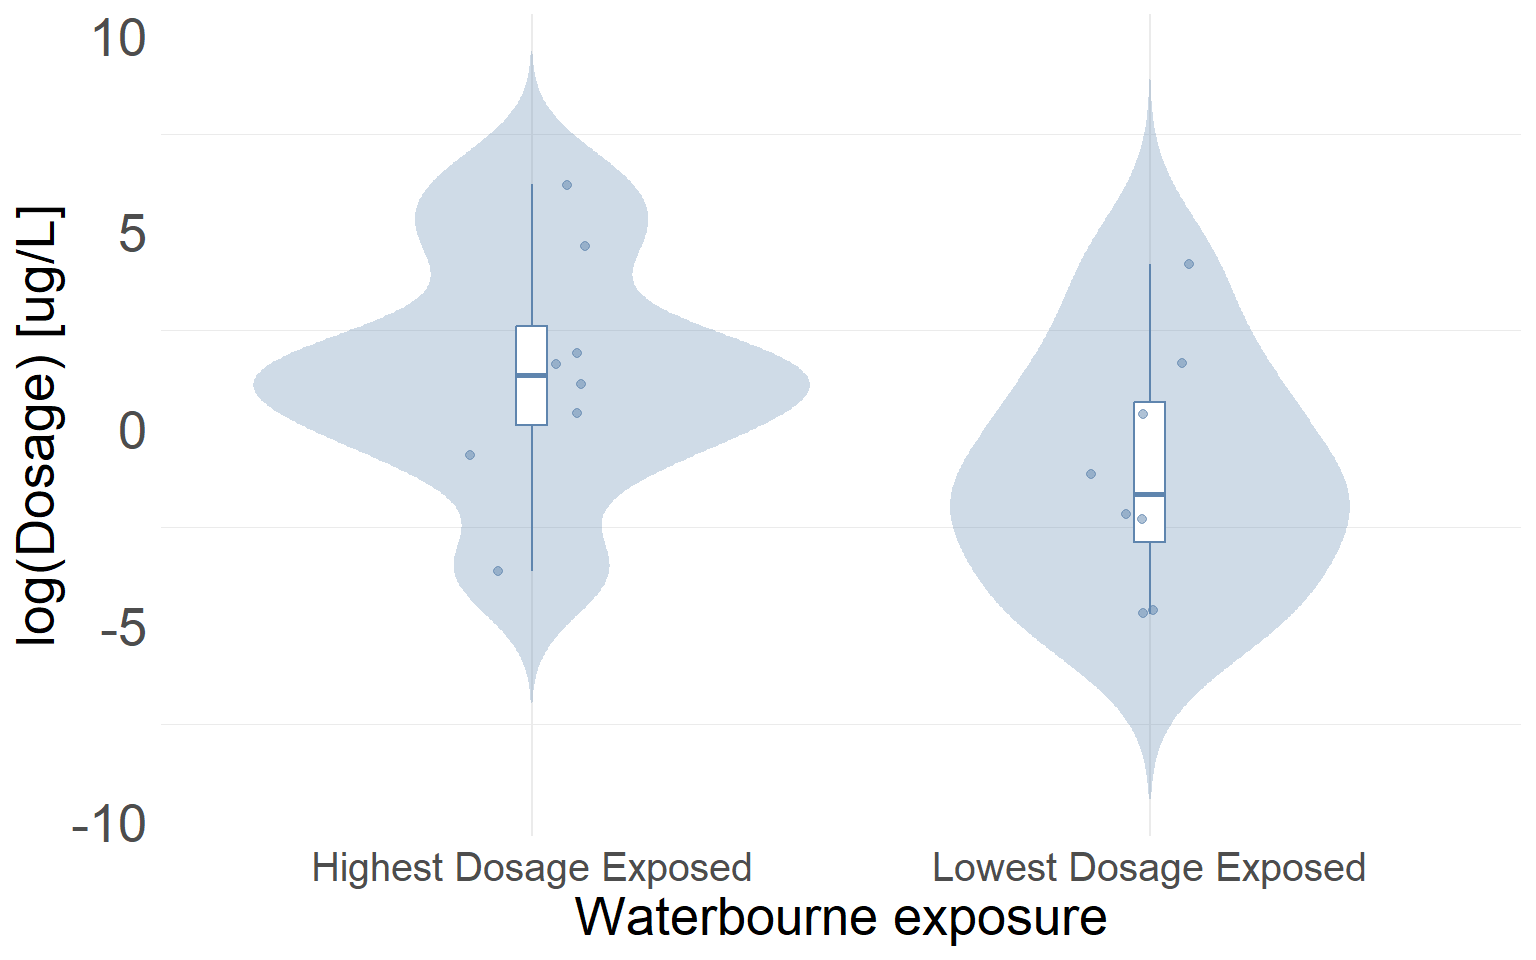
\includegraphics{zf_sm_code_files/figure-latex/unnamed-chunk-17-1.pdf}

\hypertarget{figs10---total-lifestage-of-behaviour-completed-as-a-percentage}{%
\subsection{figs10 - total lifestage of behaviour completed as a
percentage}\label{figs10---total-lifestage-of-behaviour-completed-as-a-percentage}}

\begin{Shaded}
\begin{Highlighting}[]
\CommentTok{\# Calculate total count for each category}
\NormalTok{total\_count\_lsb }\OtherTok{\textless{}{-}}\NormalTok{ sd }\SpecialCharTok{\%\textgreater{}\%} \FunctionTok{count}\NormalTok{(life\_stage\_behaviour)}

\CommentTok{\# Calculate proportion and percentage for each category}
\NormalTok{life\_stage\_pct }\OtherTok{\textless{}{-}}\NormalTok{ sd }\SpecialCharTok{\%\textgreater{}\%}
  \FunctionTok{separate\_rows}\NormalTok{(life\_stage\_behaviour, }\AttributeTok{sep =} \StringTok{",}\SpecialCharTok{\textbackslash{}\textbackslash{}}\StringTok{s*"}\NormalTok{) }\SpecialCharTok{\%\textgreater{}\%} 
  \FunctionTok{count}\NormalTok{(life\_stage\_behaviour) }\SpecialCharTok{\%\textgreater{}\%}
  \FunctionTok{mutate}\NormalTok{( }\AttributeTok{proportion =}\NormalTok{ n }\SpecialCharTok{/} \FunctionTok{sum}\NormalTok{(total\_count\_lsb}\SpecialCharTok{$}\NormalTok{n),}
    \AttributeTok{percentage =}\NormalTok{ proportion }\SpecialCharTok{*} \DecValTok{100}\NormalTok{)}

\CommentTok{\# Create a bar chart with the count on the x{-}axis and life stage of behavior on the y{-}axis}
\NormalTok{figs10 }\OtherTok{\textless{}{-}} \FunctionTok{ggplot}\NormalTok{(life\_stage\_pct, }\FunctionTok{aes}\NormalTok{(}\AttributeTok{x =} \FunctionTok{reorder}\NormalTok{(life\_stage\_behaviour, percentage), }\AttributeTok{y =}\NormalTok{ percentage)) }\SpecialCharTok{+}
  
  \CommentTok{\# Customize the appearance of the bars }
  \FunctionTok{geom\_bar}\NormalTok{(}\AttributeTok{stat =} \StringTok{"identity"}\NormalTok{, }\AttributeTok{fill =} \StringTok{"\#5F85AE"}\NormalTok{, }\AttributeTok{color =} \StringTok{"white"}\NormalTok{, }\AttributeTok{alpha =} \FloatTok{0.8}\NormalTok{,}\AttributeTok{position =} \FunctionTok{position\_dodge}\NormalTok{(}\FloatTok{0.9}\NormalTok{)) }\SpecialCharTok{+}
  
  \CommentTok{\# Add labels to the bars for percentage }
  \FunctionTok{geom\_text}\NormalTok{(}\FunctionTok{aes}\NormalTok{(}\AttributeTok{label =} \FunctionTok{paste0}\NormalTok{(}\FunctionTok{round}\NormalTok{(percentage, }\DecValTok{1}\NormalTok{), }\StringTok{"\%"}\NormalTok{)), }\AttributeTok{hjust =} \SpecialCharTok{{-}}\FloatTok{0.2}\NormalTok{, }\AttributeTok{vjust =} \FloatTok{0.5}\NormalTok{, }\AttributeTok{size =} \DecValTok{5}\NormalTok{, }\AttributeTok{fontface =} \StringTok{"bold"}\NormalTok{) }\SpecialCharTok{+}
  
  \CommentTok{\# Add absolute count to bars}
  \FunctionTok{geom\_text}\NormalTok{(}\FunctionTok{aes}\NormalTok{(}\AttributeTok{label =}\NormalTok{ n), }\AttributeTok{position =} \FunctionTok{position\_stack}\NormalTok{(}\AttributeTok{vjust =} \FloatTok{0.5}\NormalTok{), }\AttributeTok{color =} \StringTok{"white"}\NormalTok{,}\AttributeTok{fontface =} \StringTok{"bold"}\NormalTok{, }\AttributeTok{size =} \DecValTok{5}\NormalTok{) }\SpecialCharTok{+}
  
  \CommentTok{\# Add axis and plot labels }
  \FunctionTok{labs}\NormalTok{(}\AttributeTok{x =} \StringTok{"Life Stage of Behavior"}\NormalTok{, }\AttributeTok{y =} \StringTok{"Percentage"}\NormalTok{, }\AttributeTok{fontsize =} \DecValTok{14}\NormalTok{) }\SpecialCharTok{+}
  
  \CommentTok{\# Customize the plot theme }
  \FunctionTok{theme\_minimal}\NormalTok{() }\SpecialCharTok{+}
  \FunctionTok{theme}\NormalTok{(}\AttributeTok{panel.grid.major.y =} \FunctionTok{element\_blank}\NormalTok{(),}
    \AttributeTok{axis.line.y =} \FunctionTok{element\_blank}\NormalTok{(),}
    \AttributeTok{axis.ticks.y =} \FunctionTok{element\_blank}\NormalTok{(),}
    \AttributeTok{axis.text.x =} \FunctionTok{element\_text}\NormalTok{(}\AttributeTok{size =} \DecValTok{15}\NormalTok{),}
    \AttributeTok{axis.text.y =} \FunctionTok{element\_text}\NormalTok{(}\AttributeTok{size =} \DecValTok{15}\NormalTok{, }\AttributeTok{hjust =} \DecValTok{1}\NormalTok{),}
    \AttributeTok{axis.title.x =} \FunctionTok{element\_text}\NormalTok{(}\AttributeTok{size =} \DecValTok{15}\NormalTok{),}
    \AttributeTok{axis.title.y =} \FunctionTok{element\_text}\NormalTok{(}\AttributeTok{size =} \DecValTok{15}\NormalTok{),}
    \AttributeTok{plot.title =} \FunctionTok{element\_blank}\NormalTok{()) }\SpecialCharTok{+}
  \FunctionTok{coord\_flip}\NormalTok{() }\SpecialCharTok{+} 
  \FunctionTok{ylim}\NormalTok{(}\DecValTok{0}\NormalTok{, }\DecValTok{100}\NormalTok{)}

\NormalTok{figs10}
\end{Highlighting}
\end{Shaded}

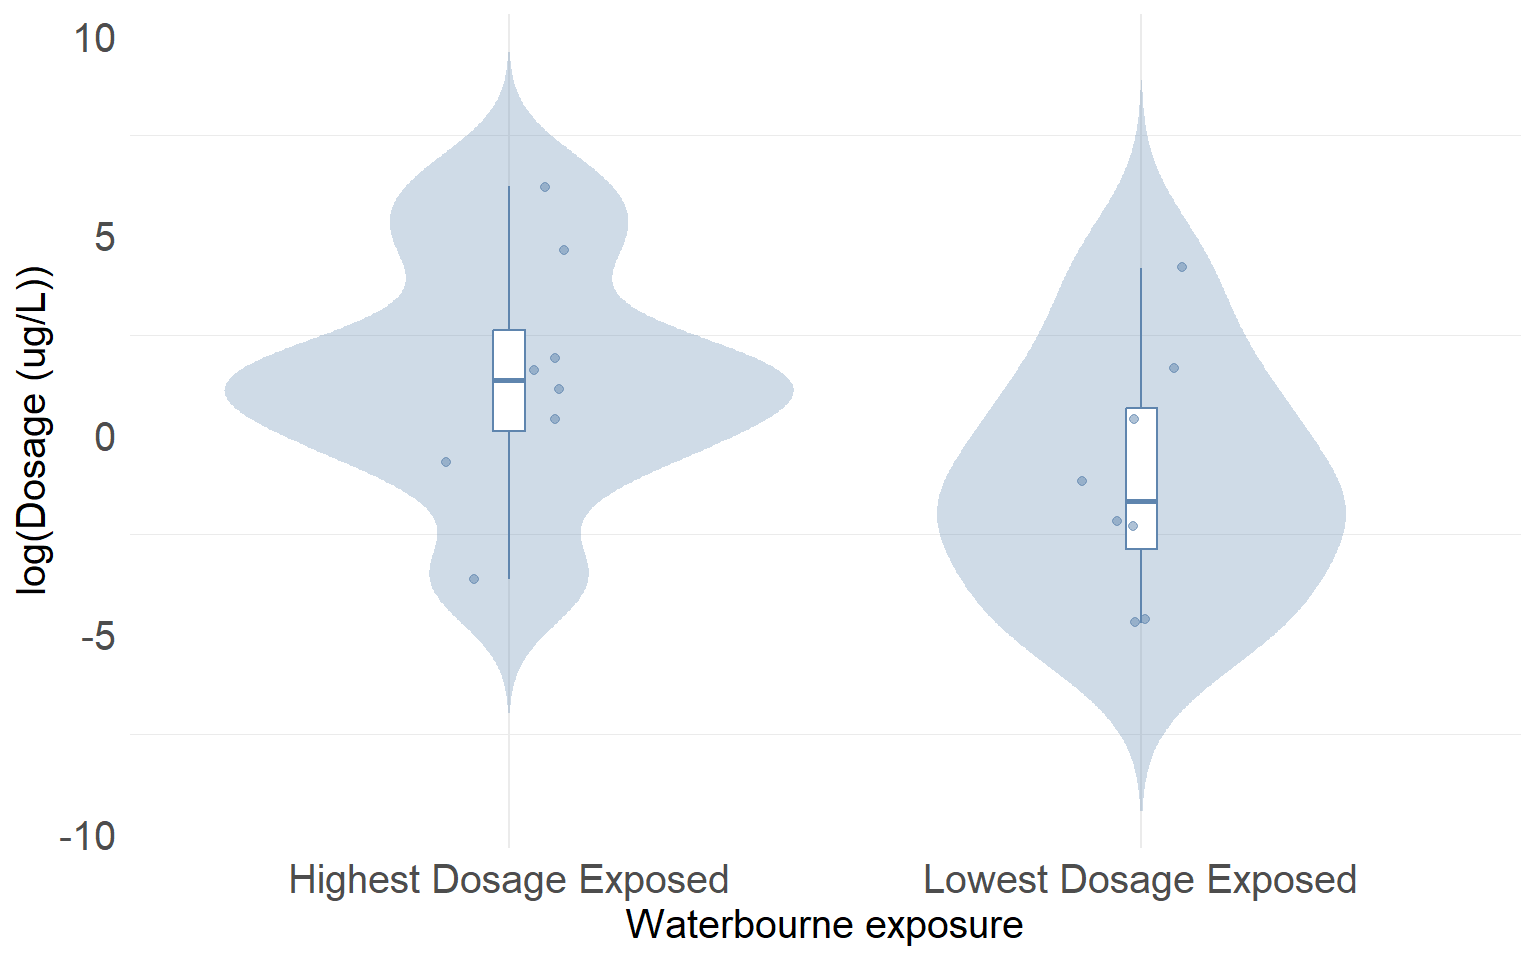
\includegraphics{zf_sm_code_files/figure-latex/unnamed-chunk-18-1.pdf}

\hypertarget{figs11---total-sexes-exposed-completed-as-a-percentage}{%
\subsection{figs11 - total sexes exposed completed as a
percentage}\label{figs11---total-sexes-exposed-completed-as-a-percentage}}

\begin{Shaded}
\begin{Highlighting}[]
\CommentTok{\# Calculate total count for each category}
\NormalTok{total\_sex\_count }\OtherTok{\textless{}{-}}\NormalTok{ sd }\SpecialCharTok{\%\textgreater{}\%} \FunctionTok{count}\NormalTok{(sex)}

\CommentTok{\# Calculate proportion and percentage for each category}
\NormalTok{sex\_pct }\OtherTok{\textless{}{-}}\NormalTok{ sd }\SpecialCharTok{\%\textgreater{}\%}
  \FunctionTok{count}\NormalTok{(sex) }\SpecialCharTok{\%\textgreater{}\%}
  \FunctionTok{mutate}\NormalTok{(}\AttributeTok{proportion =}\NormalTok{ n}\SpecialCharTok{/}\FunctionTok{sum}\NormalTok{(total\_sex\_count}\SpecialCharTok{$}\NormalTok{n),}
         \AttributeTok{percentage =}\NormalTok{ proportion}\SpecialCharTok{*}\DecValTok{100}\NormalTok{)}

\CommentTok{\# Create a bar chart with the count  on the x{-}axis and behaviorual class on the y{-}axis}
\NormalTok{figs11 }\OtherTok{\textless{}{-}} \FunctionTok{ggplot}\NormalTok{(sex\_pct, }\FunctionTok{aes}\NormalTok{(}\AttributeTok{x =} \FunctionTok{reorder}\NormalTok{(sex, percentage), }\AttributeTok{y =}\NormalTok{ percentage)) }\SpecialCharTok{+}
  
  \CommentTok{\# Customize the appearance of the bars }
  \FunctionTok{geom\_bar}\NormalTok{(}\AttributeTok{stat =} \StringTok{"identity"}\NormalTok{, }\AttributeTok{fill =} \StringTok{"\#5F85AE"}\NormalTok{, }\AttributeTok{color =} \StringTok{"white"}\NormalTok{, }\AttributeTok{alpha =} \FloatTok{0.8}\NormalTok{, }\AttributeTok{position =} \FunctionTok{position\_dodge}\NormalTok{(}\FloatTok{0.9}\NormalTok{)) }\SpecialCharTok{+}
  
  \CommentTok{\# Add labels to the bars for percentage }
  \FunctionTok{geom\_text}\NormalTok{(}\FunctionTok{aes}\NormalTok{(}\AttributeTok{label =} \FunctionTok{paste0}\NormalTok{(}\FunctionTok{round}\NormalTok{(percentage, }\DecValTok{1}\NormalTok{), }\StringTok{"\%"}\NormalTok{)), }\AttributeTok{hjust =} \SpecialCharTok{{-}}\FloatTok{0.2}\NormalTok{, }\AttributeTok{vjust =} \FloatTok{0.5}\NormalTok{, }\AttributeTok{size =} \DecValTok{5}\NormalTok{, }\AttributeTok{fontface =} \StringTok{"bold"}\NormalTok{) }\SpecialCharTok{+}
  
  \CommentTok{\# Add absolute count to bars}
  \FunctionTok{geom\_text}\NormalTok{(}\FunctionTok{aes}\NormalTok{(}\AttributeTok{label =}\NormalTok{ n), }\AttributeTok{position =} \FunctionTok{position\_stack}\NormalTok{(}\AttributeTok{vjust =} \FloatTok{0.5}\NormalTok{), }\AttributeTok{color =} \StringTok{"white"}\NormalTok{, }\AttributeTok{fontface =} \StringTok{"bold"}\NormalTok{, }\AttributeTok{size =} \DecValTok{5}\NormalTok{) }\SpecialCharTok{+}
  
  \CommentTok{\# Add axis and plot labels }
  \FunctionTok{labs}\NormalTok{(}\AttributeTok{x =} \StringTok{"Sex of Exposure"}\NormalTok{, }\AttributeTok{y =} \StringTok{"Percentage"}\NormalTok{) }\SpecialCharTok{+}
  
  \CommentTok{\# Customize the plot theme }
   \FunctionTok{theme\_minimal}\NormalTok{() }\SpecialCharTok{+}
  \FunctionTok{theme}\NormalTok{(}\AttributeTok{panel.grid.major.y =} \FunctionTok{element\_blank}\NormalTok{(),}
    \AttributeTok{axis.line.y =} \FunctionTok{element\_blank}\NormalTok{(),}
    \AttributeTok{axis.ticks.y =} \FunctionTok{element\_blank}\NormalTok{(),}
    \AttributeTok{axis.text.x =} \FunctionTok{element\_text}\NormalTok{(}\AttributeTok{size =} \DecValTok{15}\NormalTok{),}
    \AttributeTok{axis.text.y =} \FunctionTok{element\_text}\NormalTok{(}\AttributeTok{size =} \DecValTok{15}\NormalTok{, }\AttributeTok{hjust =} \DecValTok{1}\NormalTok{),}
    \AttributeTok{axis.title.x =} \FunctionTok{element\_text}\NormalTok{(}\AttributeTok{size =} \DecValTok{15}\NormalTok{),}
    \AttributeTok{axis.title.y =} \FunctionTok{element\_text}\NormalTok{(}\AttributeTok{size =} \DecValTok{15}\NormalTok{),}
    \AttributeTok{plot.title =} \FunctionTok{element\_blank}\NormalTok{()) }\SpecialCharTok{+}
  \FunctionTok{coord\_flip}\NormalTok{() }\SpecialCharTok{+} 
  \FunctionTok{ylim}\NormalTok{(}\DecValTok{0}\NormalTok{, }\DecValTok{100}\NormalTok{)}

\NormalTok{figs11}
\end{Highlighting}
\end{Shaded}

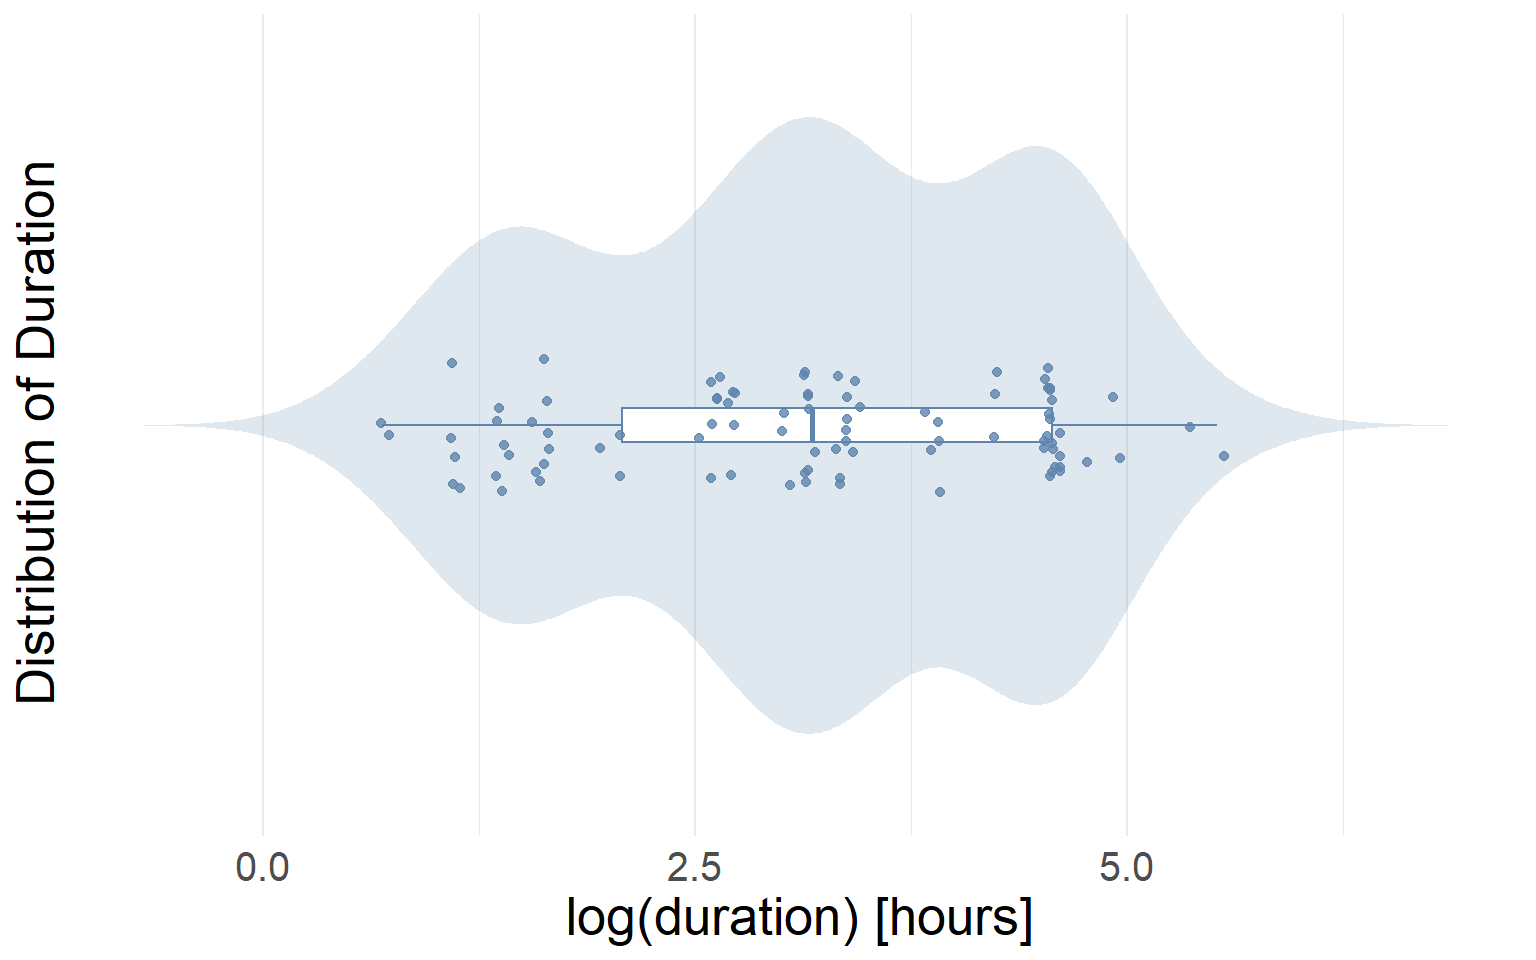
\includegraphics{zf_sm_code_files/figure-latex/unnamed-chunk-19-1.pdf}

\hypertarget{objective-3.-to-identify-the-specific-behaviours-that-have-been-investigated-in-pesticide-exposure-experiments-that-use-zebrafish-as-a-model.}{%
\section{Objective 3. To identify the specific behaviours that have been
investigated in pesticide exposure experiments that use zebrafish as a
model.}\label{objective-3.-to-identify-the-specific-behaviours-that-have-been-investigated-in-pesticide-exposure-experiments-that-use-zebrafish-as-a-model.}}

\hypertarget{fig5---total-number-of-studies-investigating-each-broad-behaviour-class}{%
\subsection{fig5 - total number of studies investigating each broad
behaviour
class}\label{fig5---total-number-of-studies-investigating-each-broad-behaviour-class}}

\begin{Shaded}
\begin{Highlighting}[]
\CommentTok{\# Calculate total count for each category}
\NormalTok{total\_behaviour\_class\_count }\OtherTok{\textless{}{-}}\NormalTok{ bd }\SpecialCharTok{\%\textgreater{}\%} 
  \FunctionTok{separate\_rows}\NormalTok{(behavioural\_class, }\AttributeTok{sep =} \StringTok{",}\SpecialCharTok{\textbackslash{}\textbackslash{}}\StringTok{s*"}\NormalTok{) }\SpecialCharTok{\%\textgreater{}\%}  
  \FunctionTok{count}\NormalTok{(behavioural\_class)}

\CommentTok{\# Calculate proportion and percentage for each category}
\NormalTok{behav\_class\_pct }\OtherTok{\textless{}{-}}\NormalTok{ total\_behaviour\_class\_count }\SpecialCharTok{\%\textgreater{}\%}
  \FunctionTok{mutate}\NormalTok{(}\AttributeTok{proportion =}\NormalTok{ n}\SpecialCharTok{/}\FunctionTok{sum}\NormalTok{(total\_behaviour\_class\_count}\SpecialCharTok{$}\NormalTok{n),}
         \AttributeTok{percentage =}\NormalTok{ proportion}\SpecialCharTok{*}\DecValTok{100}\NormalTok{)}

\CommentTok{\# Create a bar chart with the count on the x{-}axis and Behavioural class  assay on the y{-}axis}
\NormalTok{ fig5 }\OtherTok{\textless{}{-}}  \FunctionTok{ggplot}\NormalTok{(behav\_class\_pct, }\FunctionTok{aes}\NormalTok{(}\AttributeTok{x =} \FunctionTok{reorder}\NormalTok{(behavioural\_class, percentage), }\AttributeTok{y =}\NormalTok{ percentage)) }\SpecialCharTok{+}
    
  \CommentTok{\# Customize the appearance of the bars }
  \FunctionTok{geom\_bar}\NormalTok{(}\AttributeTok{stat =} \StringTok{"identity"}\NormalTok{, }\AttributeTok{fill =} \StringTok{"\#5F85AE"}\NormalTok{, }\AttributeTok{color =} \StringTok{"white"}\NormalTok{, }\AttributeTok{alpha =} \FloatTok{0.8}\NormalTok{, }\AttributeTok{position =} \FunctionTok{position\_dodge}\NormalTok{(}\FloatTok{0.9}\NormalTok{)) }\SpecialCharTok{+}
    
  \CommentTok{\# Add labels to the bars for percentage }
  \FunctionTok{geom\_text}\NormalTok{(}\FunctionTok{aes}\NormalTok{(}\AttributeTok{label =} \FunctionTok{paste0}\NormalTok{(}\FunctionTok{round}\NormalTok{(percentage, }\DecValTok{1}\NormalTok{), }\StringTok{"\%"}\NormalTok{)), }\AttributeTok{hjust =} \SpecialCharTok{{-}}\FloatTok{0.2}\NormalTok{, }\AttributeTok{vjust =} \FloatTok{0.5}\NormalTok{, }\AttributeTok{size =} \DecValTok{5}\NormalTok{, }\AttributeTok{fontface =} \StringTok{"bold"}\NormalTok{, }\AttributeTok{color =} \StringTok{"black"}\NormalTok{) }\SpecialCharTok{+}
    
  \CommentTok{\# Add labels to the bars for absolute count  }
  \FunctionTok{geom\_text}\NormalTok{(}\FunctionTok{aes}\NormalTok{(}\AttributeTok{label =}\NormalTok{ n), }\AttributeTok{position =} \FunctionTok{position\_stack}\NormalTok{(}\AttributeTok{vjust =} \FloatTok{0.5}\NormalTok{), }\AttributeTok{color =} \StringTok{"white"}\NormalTok{, }\AttributeTok{size =} \DecValTok{5}\NormalTok{, }\AttributeTok{hjust =} \FloatTok{0.5}\NormalTok{, }\AttributeTok{fontface =} \StringTok{"bold"}\NormalTok{) }\SpecialCharTok{+}
    
  \CommentTok{\# Add axis and plot labels}
  \FunctionTok{labs}\NormalTok{(}\AttributeTok{x =} \StringTok{"Behavioural Class"}\NormalTok{, }\AttributeTok{y =} \StringTok{"Percentage"}\NormalTok{) }\SpecialCharTok{+}
    
  \CommentTok{\# Customize the plot theme }
  \FunctionTok{theme\_minimal}\NormalTok{() }\SpecialCharTok{+}
  \FunctionTok{theme}\NormalTok{(}\AttributeTok{panel.grid.major.y =} \FunctionTok{element\_blank}\NormalTok{(),}
    \AttributeTok{axis.line.y =} \FunctionTok{element\_blank}\NormalTok{(),}
    \AttributeTok{axis.ticks.y =} \FunctionTok{element\_blank}\NormalTok{(),}
    \AttributeTok{axis.text.x =} \FunctionTok{element\_text}\NormalTok{(}\AttributeTok{size =} \DecValTok{15}\NormalTok{),}
    \AttributeTok{axis.text.y =} \FunctionTok{element\_text}\NormalTok{(}\AttributeTok{size =} \DecValTok{15}\NormalTok{, }\AttributeTok{hjust =} \DecValTok{1}\NormalTok{),}
    \AttributeTok{axis.title.x =} \FunctionTok{element\_text}\NormalTok{(}\AttributeTok{size =} \DecValTok{15}\NormalTok{),}
    \AttributeTok{axis.title.y =} \FunctionTok{element\_text}\NormalTok{(}\AttributeTok{size =} \DecValTok{15}\NormalTok{),}
    \AttributeTok{plot.title =} \FunctionTok{element\_blank}\NormalTok{()) }\SpecialCharTok{+}
   \FunctionTok{coord\_flip}\NormalTok{() }\SpecialCharTok{+} 
   \FunctionTok{ylim}\NormalTok{(}\DecValTok{0}\NormalTok{, }\DecValTok{50}\NormalTok{)}
  
  
\NormalTok{fig5}
\end{Highlighting}
\end{Shaded}

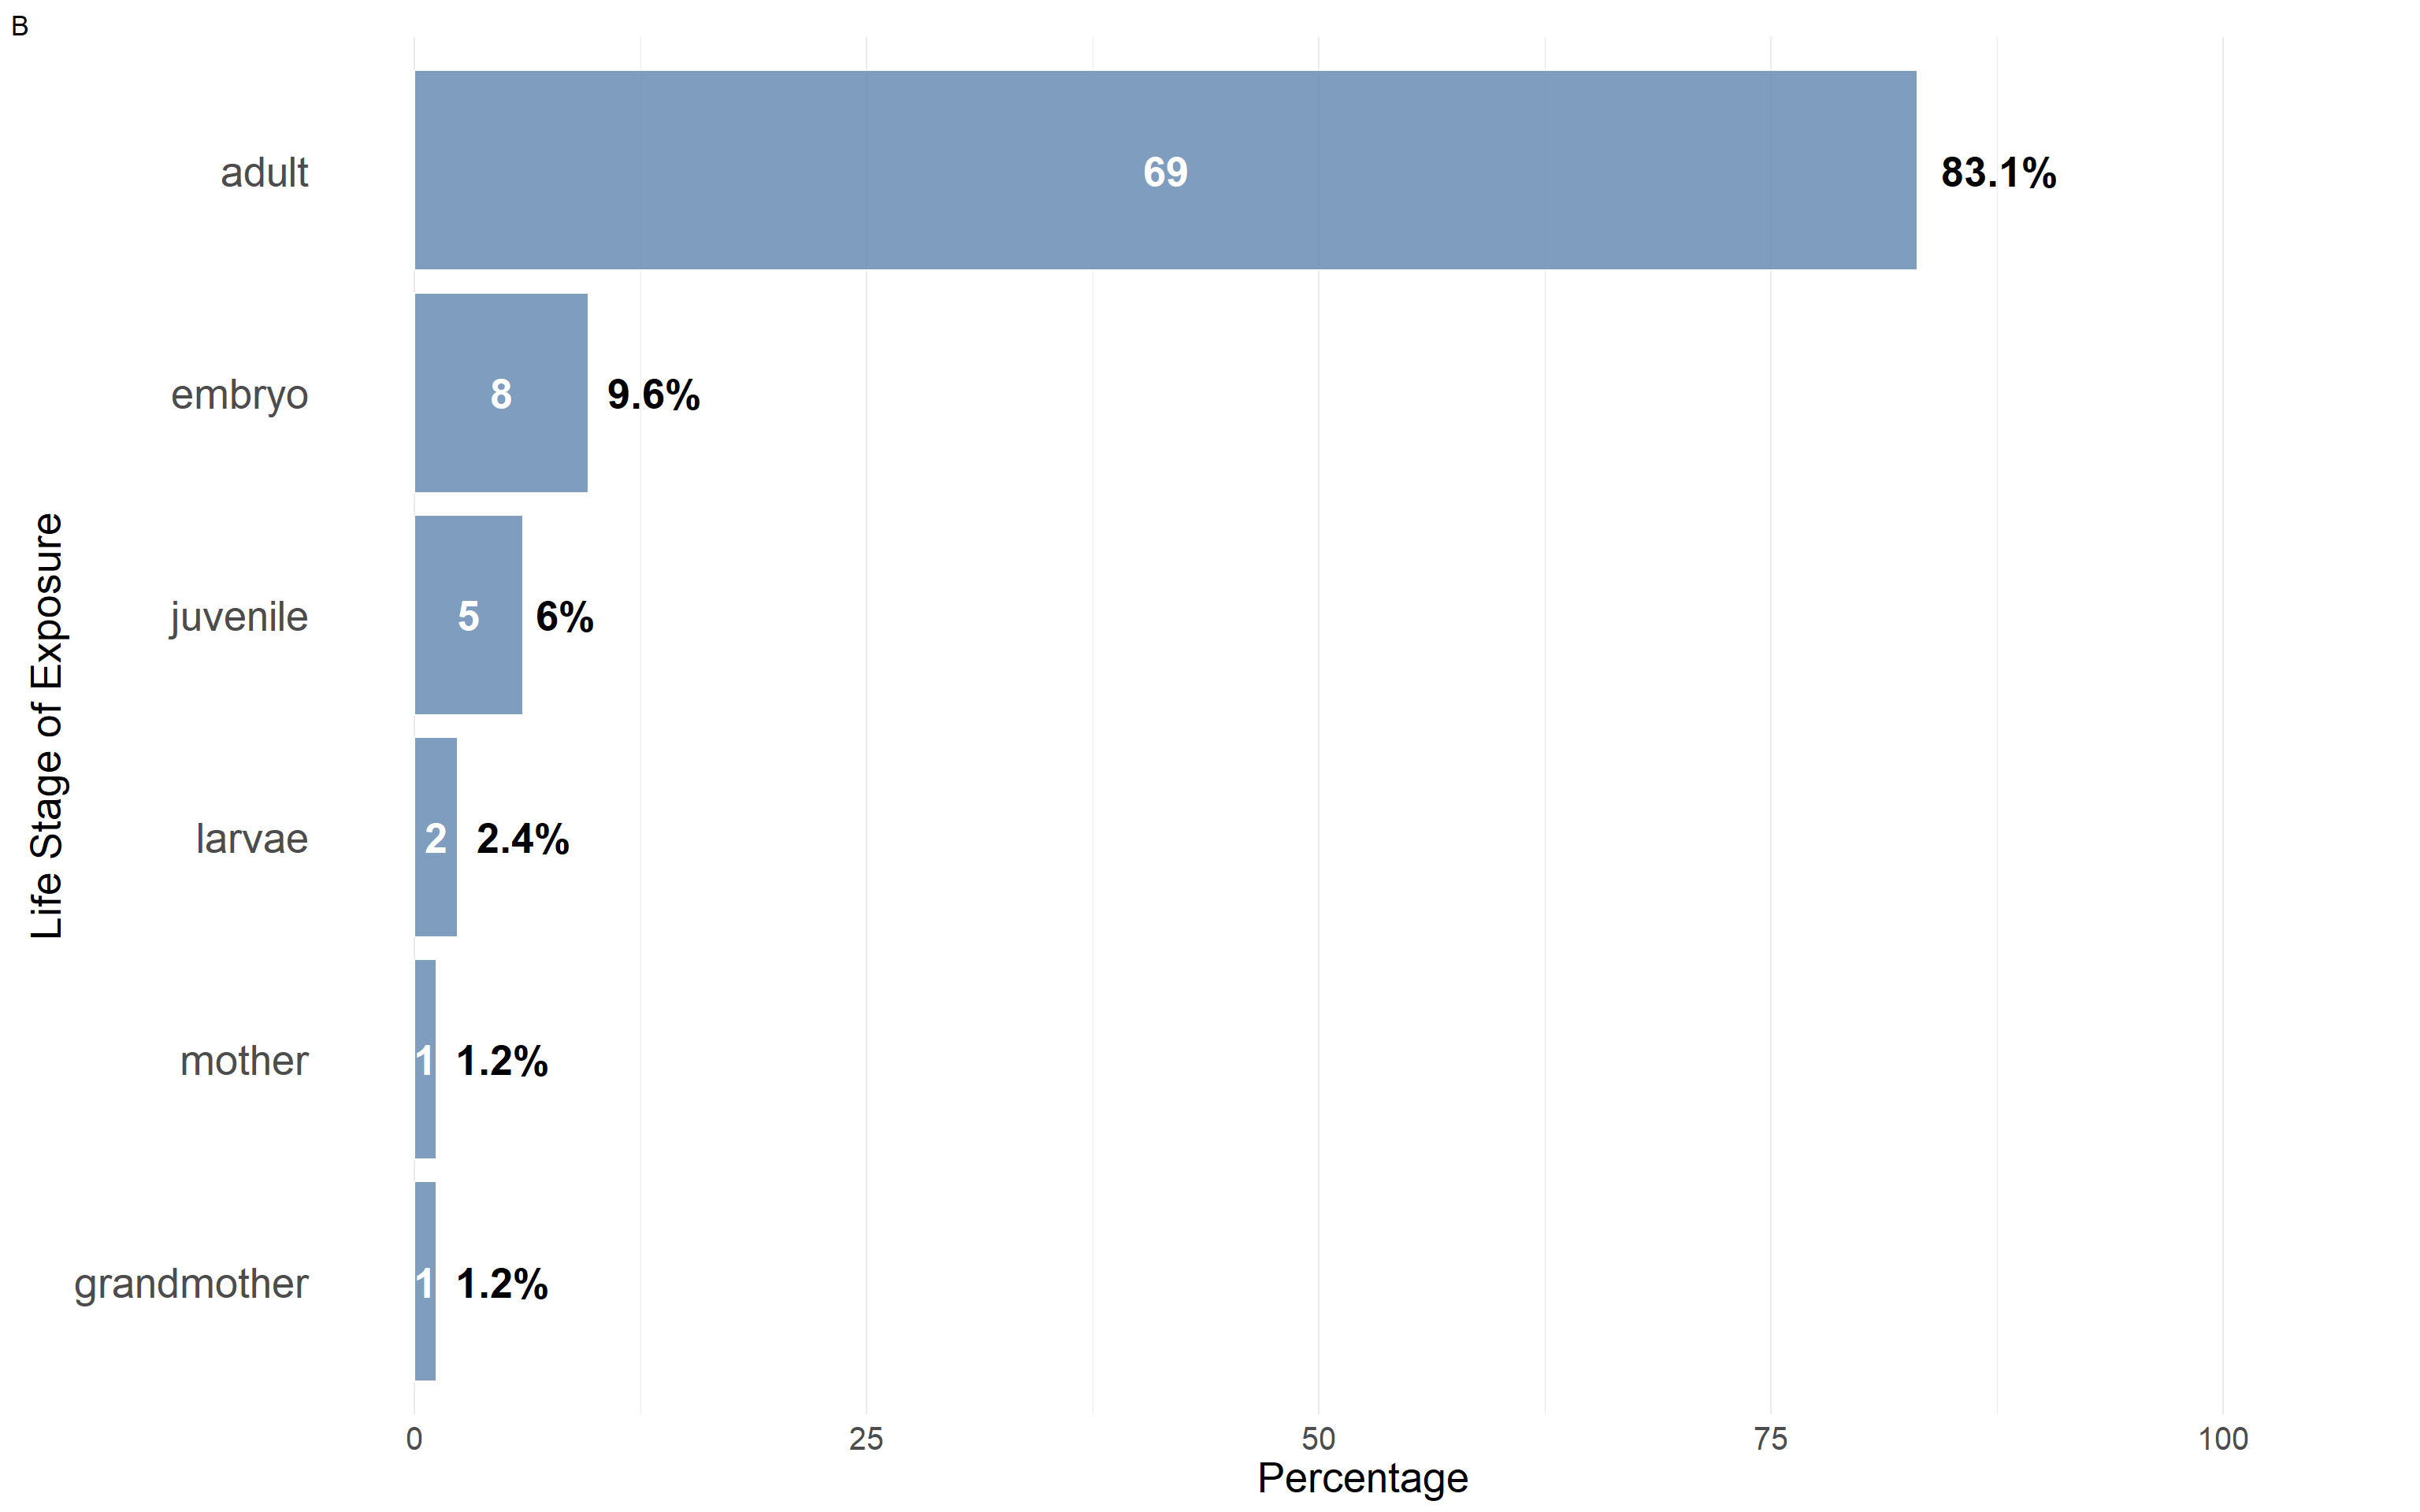
\includegraphics{zf_sm_code_files/figure-latex/unnamed-chunk-20-1.pdf}

\hypertarget{figs12---total-number-of-studies-investigating-each-behavioural-assay-of-behaviour-activity}{%
\subsection{figs12 - total number of studies investigating each
behavioural assay of behaviour
activity}\label{figs12---total-number-of-studies-investigating-each-behavioural-assay-of-behaviour-activity}}

\begin{Shaded}
\begin{Highlighting}[]
\CommentTok{\# Calculate count for each assay in behavioral activity }
\NormalTok{total\_behaviour\_activity\_count }\OtherTok{\textless{}{-}}\NormalTok{ bd }\SpecialCharTok{\%\textgreater{}\%} 
  \FunctionTok{separate\_rows}\NormalTok{(behaviour\_activity, }\AttributeTok{sep =} \StringTok{",}\SpecialCharTok{\textbackslash{}\textbackslash{}}\StringTok{s*"}\NormalTok{) }\SpecialCharTok{\%\textgreater{}\%}  
  \FunctionTok{count}\NormalTok{(behaviour\_activity) }\SpecialCharTok{\%\textgreater{}\%} 
  \FunctionTok{na.omit}\NormalTok{()}

\CommentTok{\# Calculate proportion and percentage for each category}
\NormalTok{behav\_activity\_pct }\OtherTok{\textless{}{-}}\NormalTok{ total\_behaviour\_activity\_count }\SpecialCharTok{\%\textgreater{}\%}
  \FunctionTok{mutate}\NormalTok{(}\AttributeTok{proportion =}\NormalTok{ n}\SpecialCharTok{/}\FunctionTok{sum}\NormalTok{(total\_behaviour\_activity\_count}\SpecialCharTok{$}\NormalTok{n),}
         \AttributeTok{percentage =}\NormalTok{ proportion}\SpecialCharTok{*}\DecValTok{100}\NormalTok{)}

\CommentTok{\# Create a bar chart with the count on the x{-}axis and Behavioural activity assay on the y{-}axis}
\NormalTok{figs12 }\OtherTok{\textless{}{-}}  \FunctionTok{ggplot}\NormalTok{(behav\_activity\_pct, }\FunctionTok{aes}\NormalTok{(}\AttributeTok{x =} \FunctionTok{reorder}\NormalTok{(behaviour\_activity, n), }\AttributeTok{y =}\NormalTok{ percentage)) }\SpecialCharTok{+}
  
  \CommentTok{\# Customize the appearance of the bars }
  \FunctionTok{geom\_bar}\NormalTok{(}\AttributeTok{stat =} \StringTok{"identity"}\NormalTok{, }\AttributeTok{fill =} \StringTok{"\#5F85AE"}\NormalTok{, }\AttributeTok{color =} \StringTok{"white"}\NormalTok{, }\AttributeTok{alpha =} \FloatTok{0.8}\NormalTok{, }\AttributeTok{position =} \FunctionTok{position\_dodge}\NormalTok{(}\FloatTok{0.9}\NormalTok{)) }\SpecialCharTok{+}
  
 \CommentTok{\# Add labels to the bars for percentage }
  \FunctionTok{geom\_text}\NormalTok{(}\FunctionTok{aes}\NormalTok{(}\AttributeTok{label =} \FunctionTok{paste0}\NormalTok{(}\FunctionTok{round}\NormalTok{(percentage, }\DecValTok{1}\NormalTok{), }\StringTok{"\%"}\NormalTok{)), }\AttributeTok{hjust =} \SpecialCharTok{{-}}\FloatTok{0.2}\NormalTok{, }\AttributeTok{vjust =} \FloatTok{0.5}\NormalTok{, }\AttributeTok{size =} \DecValTok{5}\NormalTok{, }\AttributeTok{fontface =} \StringTok{"bold"}\NormalTok{,     }\AttributeTok{color =} \StringTok{"black"}\NormalTok{) }\SpecialCharTok{+}
    
  \CommentTok{\# Add labels to the bars for absolute count  }
  \FunctionTok{geom\_text}\NormalTok{(}\FunctionTok{aes}\NormalTok{(}\AttributeTok{label =}\NormalTok{ n), }\AttributeTok{position =} \FunctionTok{position\_stack}\NormalTok{(}\AttributeTok{vjust =} \FloatTok{0.5}\NormalTok{), }\AttributeTok{color =} \StringTok{"white"}\NormalTok{, }\AttributeTok{size =} \DecValTok{5}\NormalTok{, }\AttributeTok{hjust =} \FloatTok{0.5}\NormalTok{, }\AttributeTok{fontface =}   \StringTok{"bold"}\NormalTok{) }\SpecialCharTok{+}
  
  \CommentTok{\# Add axis and plot labels}
  \FunctionTok{labs}\NormalTok{(}\AttributeTok{x =} \StringTok{"Activity Assay"}\NormalTok{, }\AttributeTok{y =} \StringTok{"Percentage"}\NormalTok{) }\SpecialCharTok{+}
  
  \CommentTok{\# Customize the plot theme}
  \FunctionTok{theme\_minimal}\NormalTok{() }\SpecialCharTok{+}
  \FunctionTok{theme}\NormalTok{(}\AttributeTok{panel.grid.major.y =} \FunctionTok{element\_blank}\NormalTok{(),}
    \AttributeTok{axis.line.y =} \FunctionTok{element\_blank}\NormalTok{(),}
    \AttributeTok{axis.ticks.y =} \FunctionTok{element\_blank}\NormalTok{(),}
    \AttributeTok{axis.text.x =} \FunctionTok{element\_text}\NormalTok{(}\AttributeTok{size =} \DecValTok{15}\NormalTok{),}
    \AttributeTok{axis.text.y =} \FunctionTok{element\_text}\NormalTok{(}\AttributeTok{size =} \DecValTok{15}\NormalTok{, }\AttributeTok{hjust =} \DecValTok{1}\NormalTok{),}
    \AttributeTok{axis.title.x =} \FunctionTok{element\_text}\NormalTok{(}\AttributeTok{size =} \DecValTok{15}\NormalTok{),}
    \AttributeTok{axis.title.y =} \FunctionTok{element\_text}\NormalTok{(}\AttributeTok{size =} \DecValTok{15}\NormalTok{),}
    \AttributeTok{plot.title =} \FunctionTok{element\_blank}\NormalTok{()) }\SpecialCharTok{+}
    \FunctionTok{coord\_flip}\NormalTok{() }\SpecialCharTok{+}
  \FunctionTok{ylim}\NormalTok{(}\DecValTok{0}\NormalTok{, }\DecValTok{100}\NormalTok{)}

\NormalTok{figs12}
\end{Highlighting}
\end{Shaded}

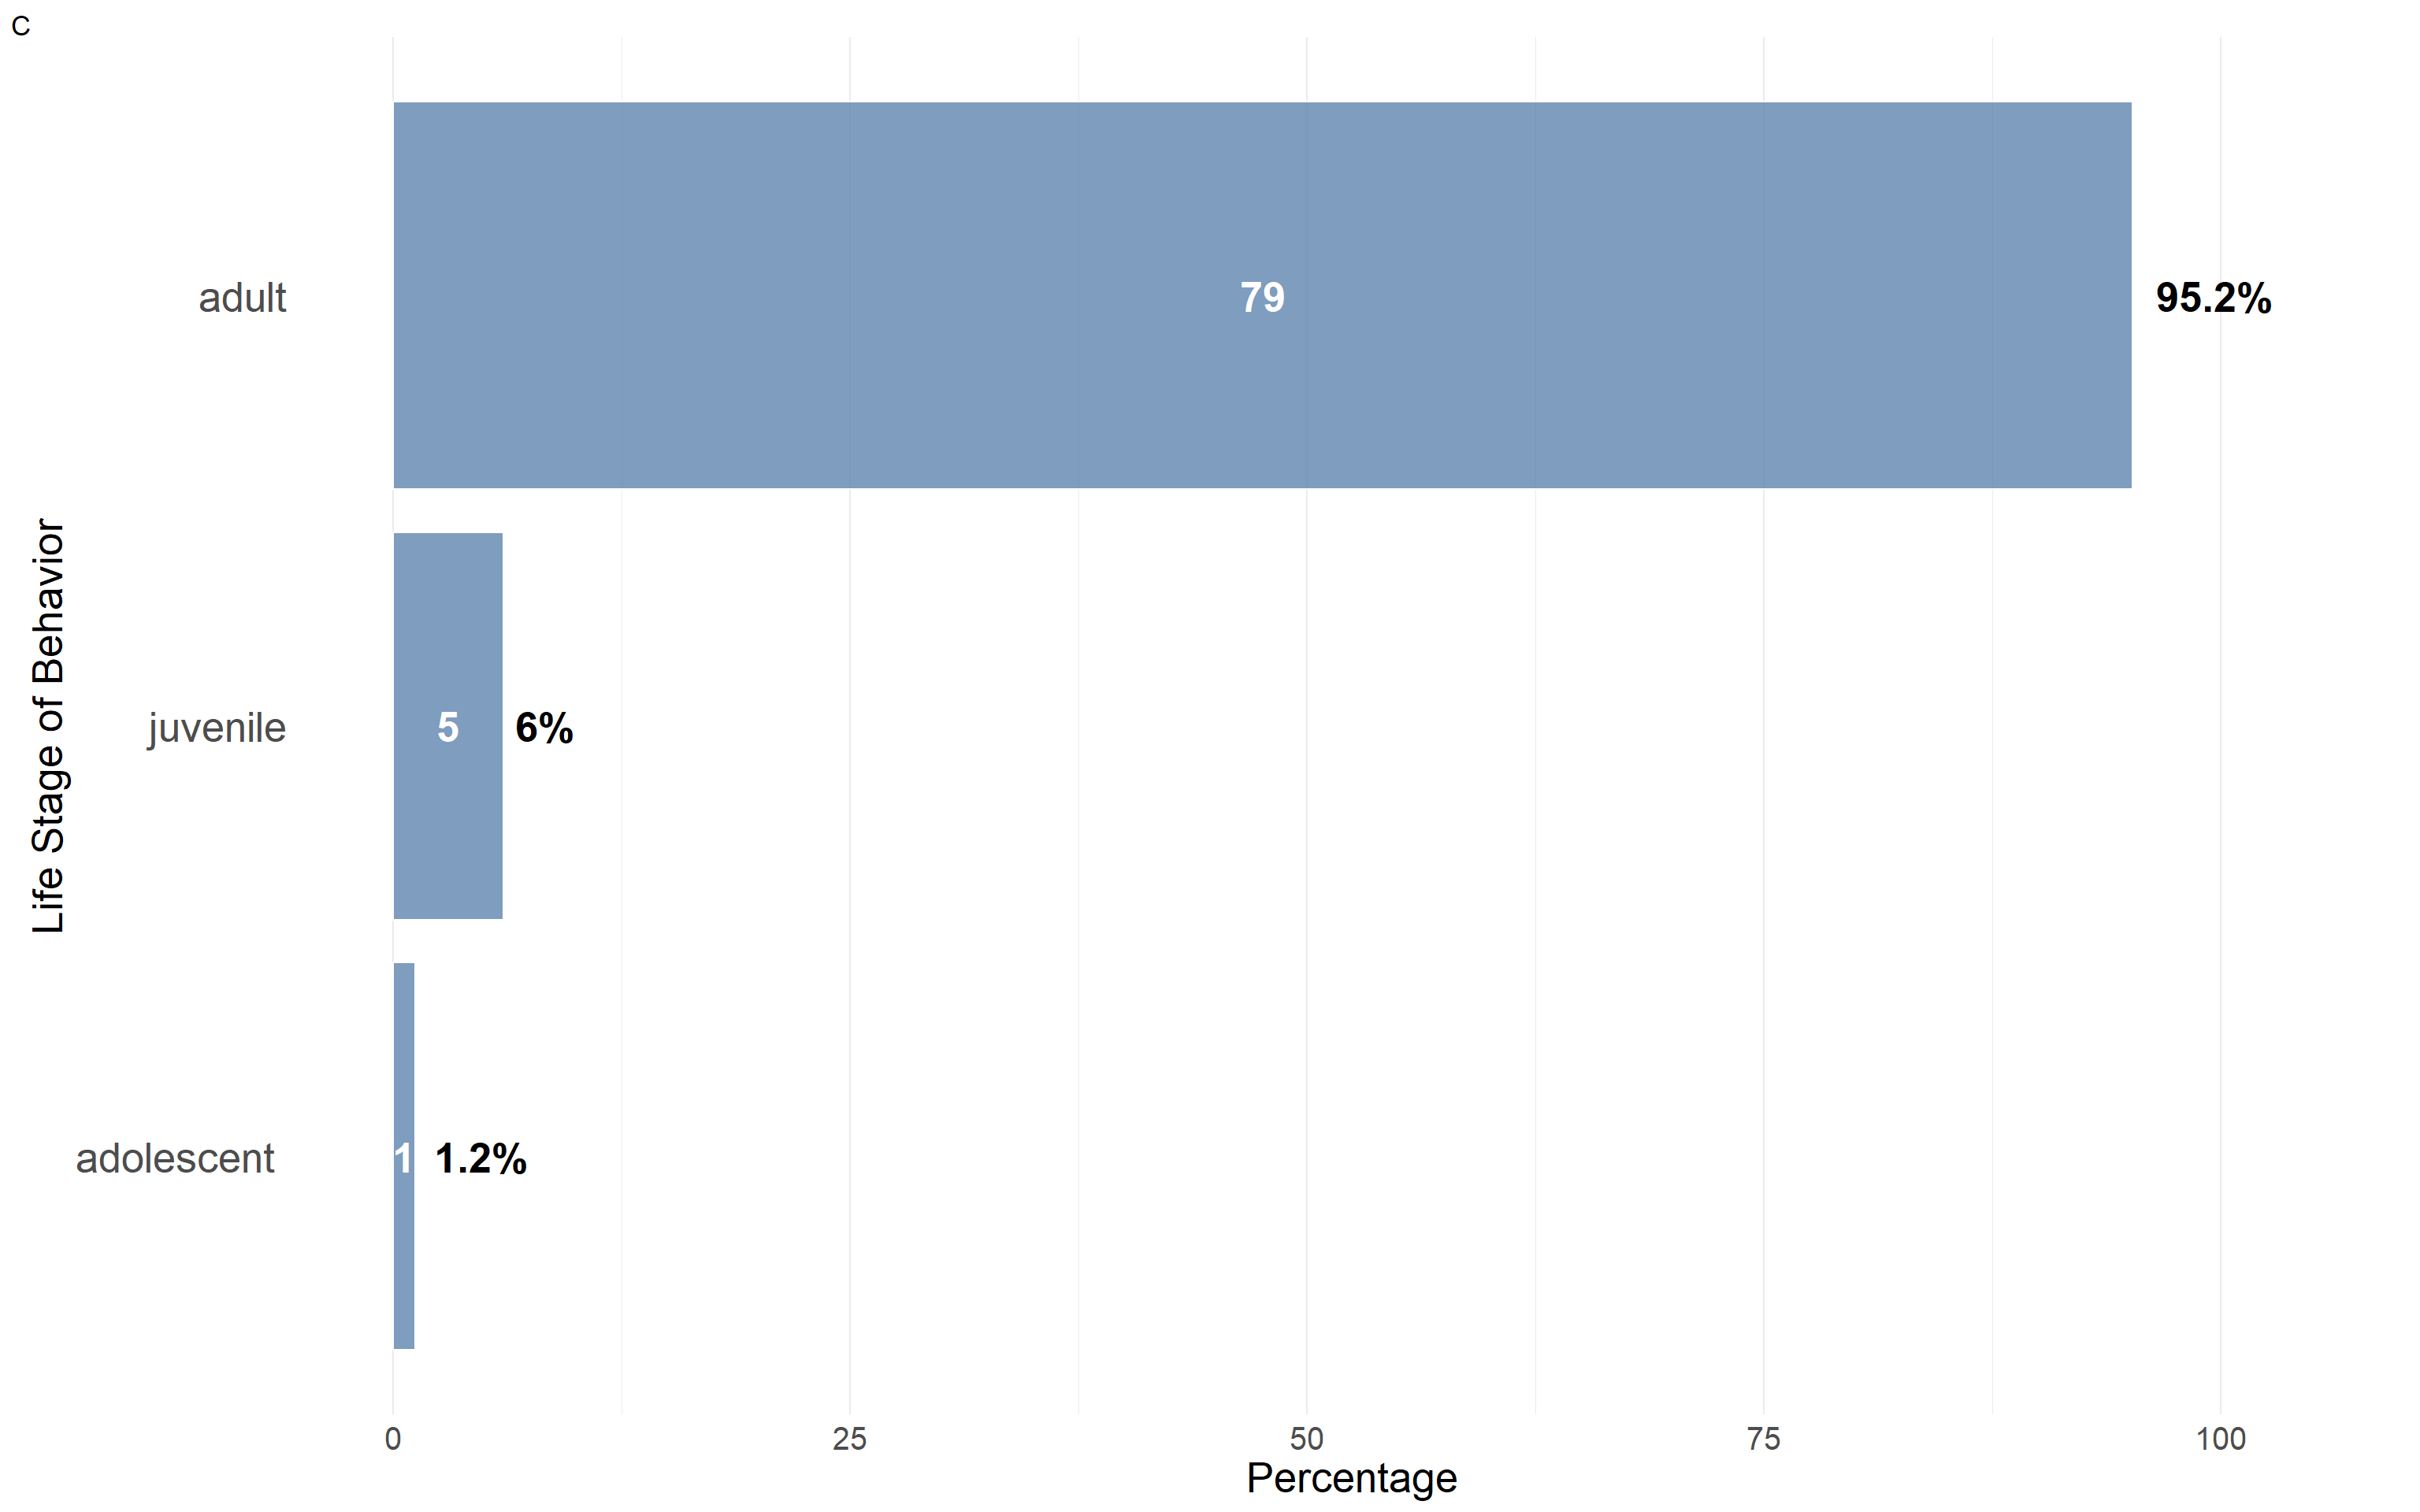
\includegraphics{zf_sm_code_files/figure-latex/unnamed-chunk-21-1.pdf}

\hypertarget{figs13---total-number-of-studies-investigating-each-behavioural-assay-of-behaviour_aggression}{%
\subsection{figs13 - total number of studies investigating each
behavioural assay of
behaviour\_aggression}\label{figs13---total-number-of-studies-investigating-each-behavioural-assay-of-behaviour_aggression}}

\begin{Shaded}
\begin{Highlighting}[]
\CommentTok{\# Calculate count for each assay in aggression behavior}
\NormalTok{total\_behaviour\_aggression\_count }\OtherTok{\textless{}{-}}\NormalTok{ bd }\SpecialCharTok{\%\textgreater{}\%} 
  \FunctionTok{separate\_rows}\NormalTok{(behaviour\_aggression, }\AttributeTok{sep =} \StringTok{",}\SpecialCharTok{\textbackslash{}\textbackslash{}}\StringTok{s*"}\NormalTok{) }\SpecialCharTok{\%\textgreater{}\%}  
  \FunctionTok{count}\NormalTok{(behaviour\_aggression) }\SpecialCharTok{\%\textgreater{}\%} 
  \FunctionTok{na.omit}\NormalTok{()}

\CommentTok{\# Calculate proportion and percentage for each category}
\NormalTok{behav\_aggression\_pct }\OtherTok{\textless{}{-}}\NormalTok{ total\_behaviour\_aggression\_count }\SpecialCharTok{\%\textgreater{}\%}
  \FunctionTok{mutate}\NormalTok{(}\AttributeTok{proportion =}\NormalTok{ n}\SpecialCharTok{/}\FunctionTok{sum}\NormalTok{(total\_behaviour\_aggression\_count}\SpecialCharTok{$}\NormalTok{n),}
         \AttributeTok{percentage =}\NormalTok{ proportion}\SpecialCharTok{*}\DecValTok{100}\NormalTok{)}

\CommentTok{\# Create a bar chart with the count on the x{-}axis and aggression behavior assay on the y{-}axis}
\NormalTok{figs13 }\OtherTok{\textless{}{-}}  \FunctionTok{ggplot}\NormalTok{(behav\_aggression\_pct, }\FunctionTok{aes}\NormalTok{(}\AttributeTok{x =} \FunctionTok{reorder}\NormalTok{(behaviour\_aggression, n), }\AttributeTok{y =}\NormalTok{ percentage)) }\SpecialCharTok{+}
  
  \CommentTok{\# Customize the appearance of the bars }
  \FunctionTok{geom\_bar}\NormalTok{(}\AttributeTok{stat =} \StringTok{"identity"}\NormalTok{, }\AttributeTok{fill =} \StringTok{"\#5F85AE"}\NormalTok{, }\AttributeTok{color =} \StringTok{"white"}\NormalTok{, }\AttributeTok{alpha =} \FloatTok{0.8}\NormalTok{, }\AttributeTok{position =} \FunctionTok{position\_dodge}\NormalTok{(}\FloatTok{0.9}\NormalTok{)) }\SpecialCharTok{+}
  
 \CommentTok{\# Add labels to the bars for percentage }
  \FunctionTok{geom\_text}\NormalTok{(}\FunctionTok{aes}\NormalTok{(}\AttributeTok{label =} \FunctionTok{paste0}\NormalTok{(}\FunctionTok{round}\NormalTok{(percentage, }\DecValTok{1}\NormalTok{), }\StringTok{"\%"}\NormalTok{)), }\AttributeTok{hjust =} \SpecialCharTok{{-}}\FloatTok{0.2}\NormalTok{, }\AttributeTok{vjust =} \FloatTok{0.5}\NormalTok{, }\AttributeTok{size =} \DecValTok{5}\NormalTok{, }\AttributeTok{fontface =} \StringTok{"bold"}\NormalTok{,     }\AttributeTok{color =} \StringTok{"black"}\NormalTok{) }\SpecialCharTok{+}
    
  \CommentTok{\# Add labels to the bars for absolute count  }
  \FunctionTok{geom\_text}\NormalTok{(}\FunctionTok{aes}\NormalTok{(}\AttributeTok{label =}\NormalTok{ n), }\AttributeTok{position =} \FunctionTok{position\_stack}\NormalTok{(}\AttributeTok{vjust =} \FloatTok{0.5}\NormalTok{), }\AttributeTok{color =} \StringTok{"white"}\NormalTok{, }\AttributeTok{size =} \DecValTok{5}\NormalTok{, }\AttributeTok{hjust =} \FloatTok{0.5}\NormalTok{, }\AttributeTok{fontface =}   \StringTok{"bold"}\NormalTok{) }\SpecialCharTok{+}
  
  \CommentTok{\# Add axis and plot labels}
  \FunctionTok{labs}\NormalTok{(}\AttributeTok{x =} \StringTok{"Aggression Behavior Assay"}\NormalTok{, }\AttributeTok{y =} \StringTok{"Percentage"}\NormalTok{) }\SpecialCharTok{+}
  
  \CommentTok{\# Customize the plot theme}
  \FunctionTok{theme\_minimal}\NormalTok{() }\SpecialCharTok{+}
  \FunctionTok{theme}\NormalTok{(}\AttributeTok{panel.grid.major.y =} \FunctionTok{element\_blank}\NormalTok{(),}
    \AttributeTok{axis.line.y =} \FunctionTok{element\_blank}\NormalTok{(),}
    \AttributeTok{axis.ticks.y =} \FunctionTok{element\_blank}\NormalTok{(),}
    \AttributeTok{axis.text.x =} \FunctionTok{element\_text}\NormalTok{(}\AttributeTok{size =} \DecValTok{15}\NormalTok{),}
    \AttributeTok{axis.text.y =} \FunctionTok{element\_text}\NormalTok{(}\AttributeTok{size =} \DecValTok{15}\NormalTok{, }\AttributeTok{hjust =} \DecValTok{1}\NormalTok{),}
    \AttributeTok{axis.title.x =} \FunctionTok{element\_text}\NormalTok{(}\AttributeTok{size =} \DecValTok{15}\NormalTok{),}
    \AttributeTok{axis.title.y =} \FunctionTok{element\_text}\NormalTok{(}\AttributeTok{size =} \DecValTok{15}\NormalTok{),}
    \AttributeTok{plot.title =} \FunctionTok{element\_blank}\NormalTok{()) }\SpecialCharTok{+}
    \FunctionTok{coord\_flip}\NormalTok{() }\SpecialCharTok{+}
  \FunctionTok{ylim}\NormalTok{(}\DecValTok{0}\NormalTok{, }\DecValTok{120}\NormalTok{)}

\NormalTok{figs13}
\end{Highlighting}
\end{Shaded}

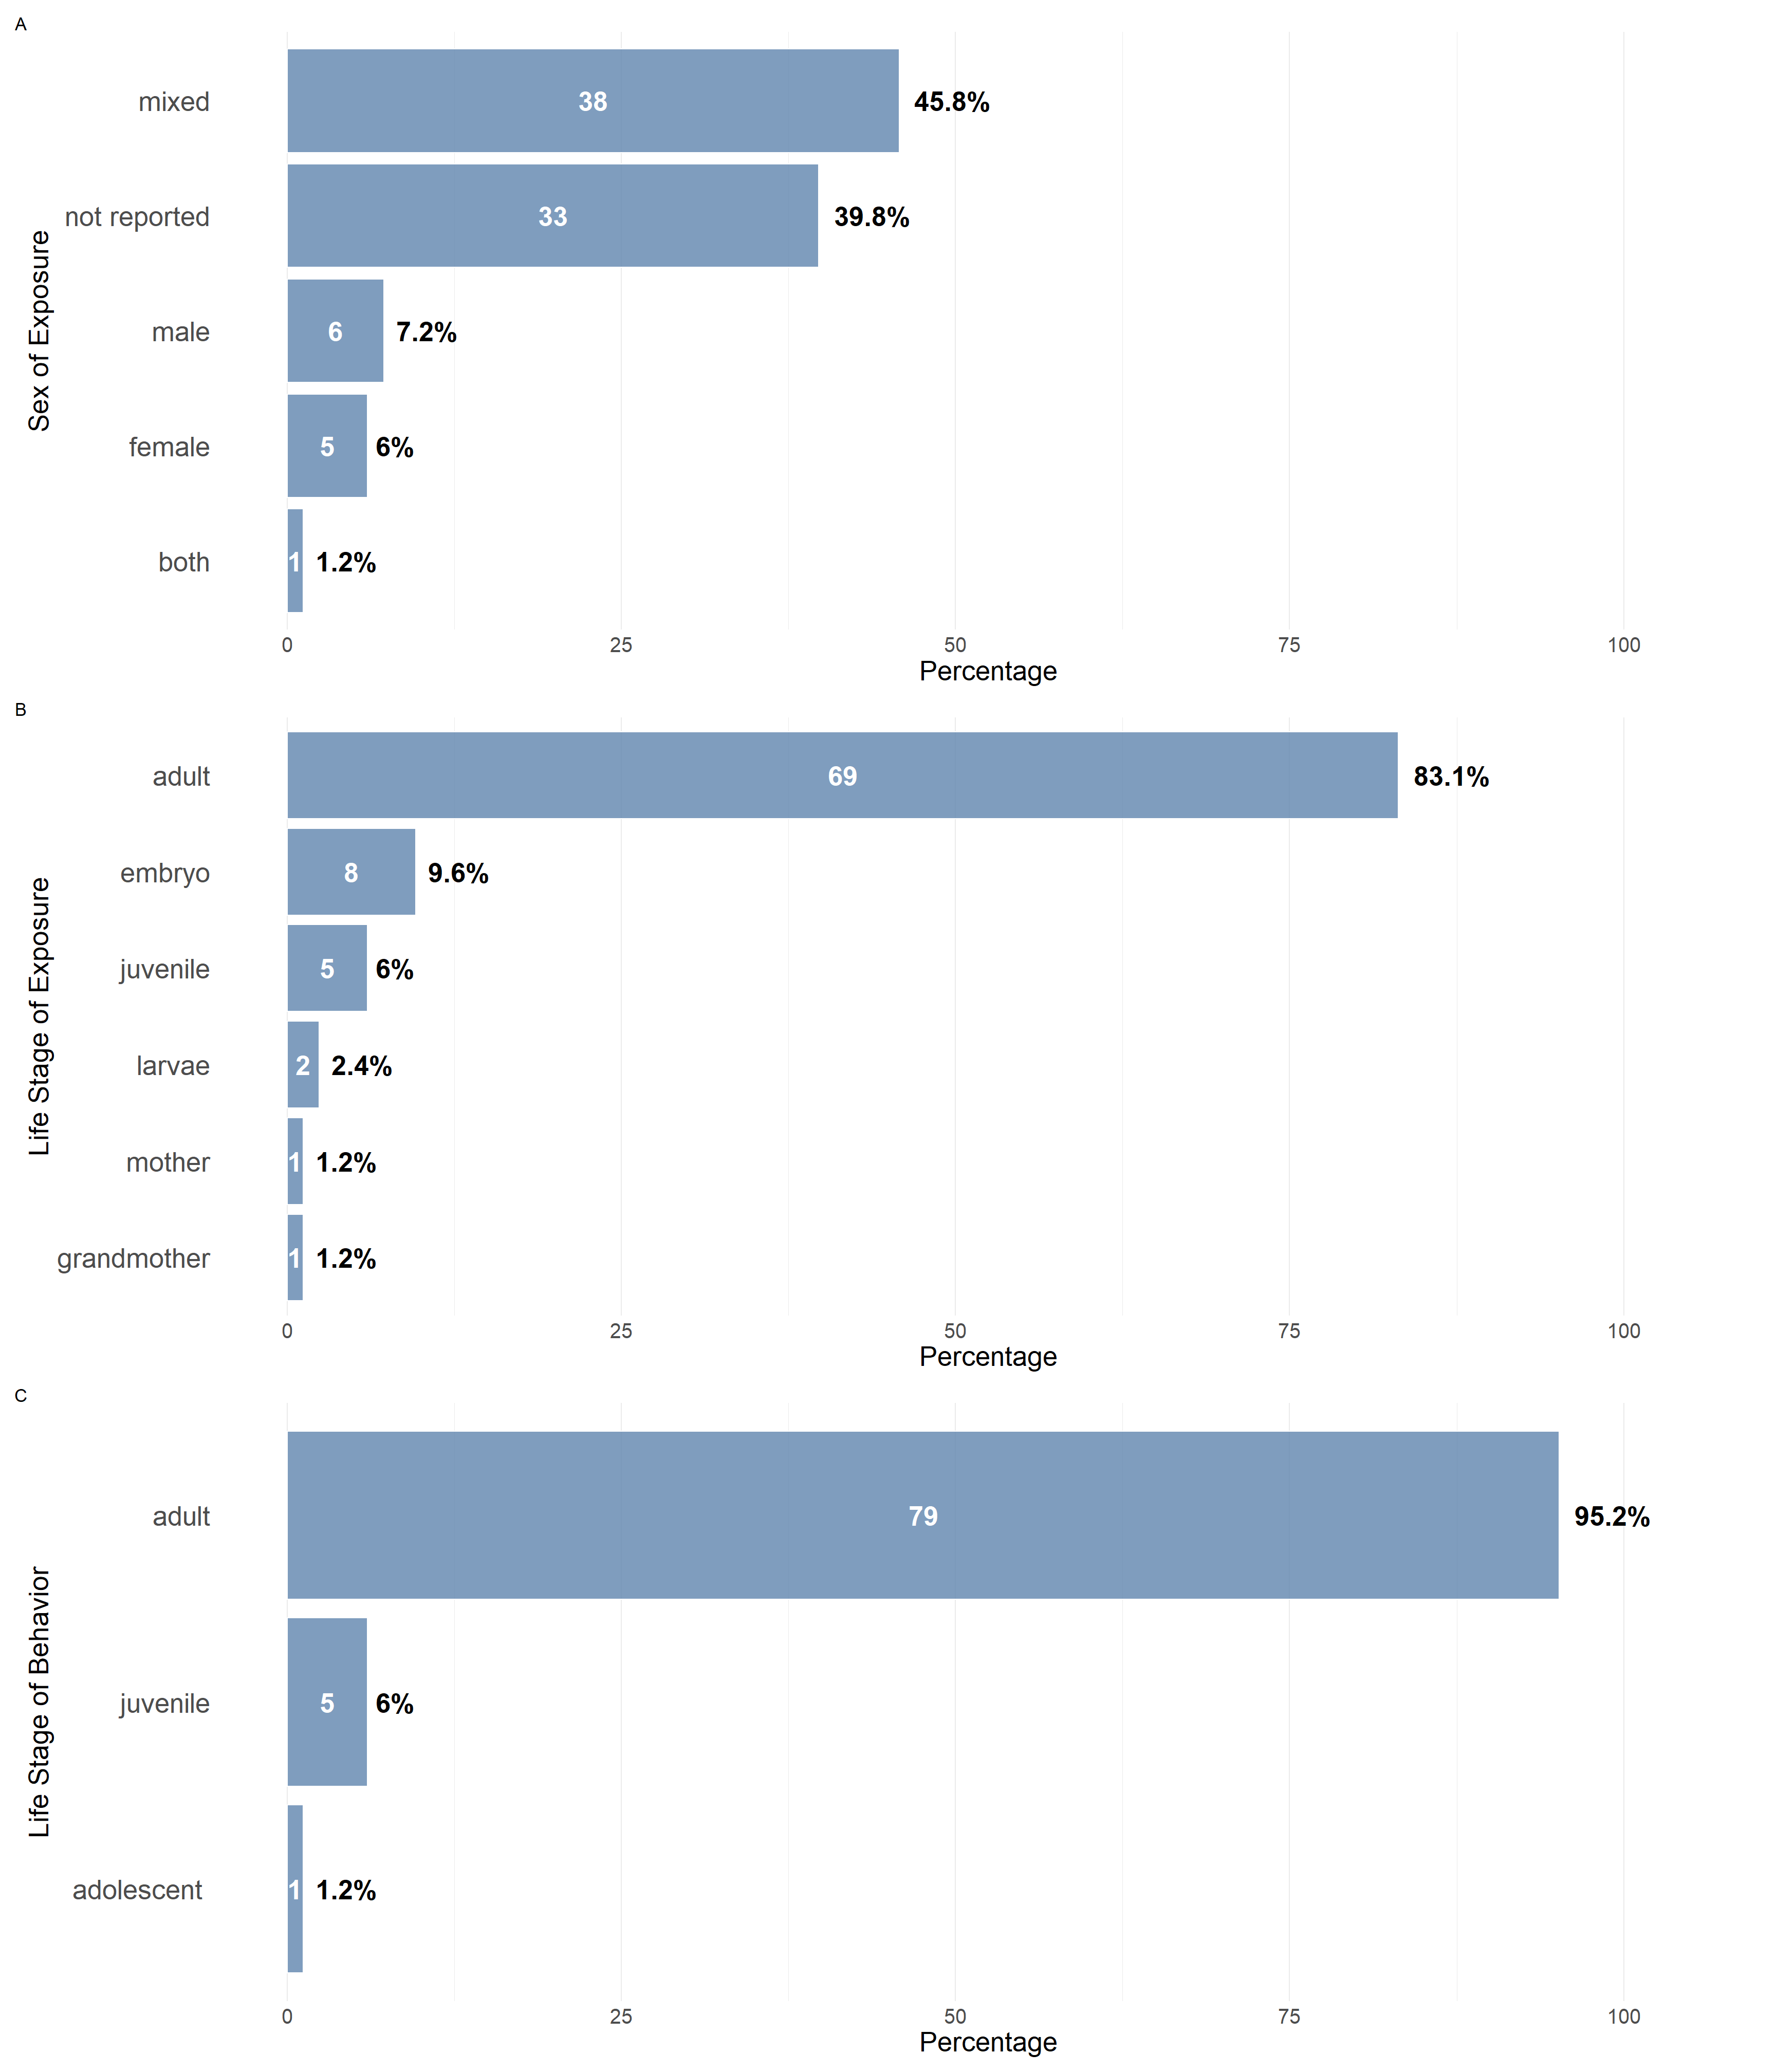
\includegraphics{zf_sm_code_files/figure-latex/unnamed-chunk-22-1.pdf}

\hypertarget{figs14---total-number-of-studies-investigating-each-behavioural-assay-of-behavioural_sociality}{%
\subsection{figs14 - total number of studies investigating each
behavioural assay of
behavioural\_sociality}\label{figs14---total-number-of-studies-investigating-each-behavioural-assay-of-behavioural_sociality}}

\begin{Shaded}
\begin{Highlighting}[]
\CommentTok{\# Calculate count for each assay in social behavior}
\NormalTok{total\_behaviour\_sociality\_count }\OtherTok{\textless{}{-}}\NormalTok{ bd }\SpecialCharTok{\%\textgreater{}\%} 
  \FunctionTok{separate\_rows}\NormalTok{(behaviour\_sociality, }\AttributeTok{sep =} \StringTok{",}\SpecialCharTok{\textbackslash{}\textbackslash{}}\StringTok{s*"}\NormalTok{) }\SpecialCharTok{\%\textgreater{}\%}  
  \FunctionTok{count}\NormalTok{(behaviour\_sociality) }\SpecialCharTok{\%\textgreater{}\%} 
  \FunctionTok{na.omit}\NormalTok{()}

\CommentTok{\# Calculate proportion and percentage for each category}
\NormalTok{behav\_sociality\_pct }\OtherTok{\textless{}{-}}\NormalTok{ total\_behaviour\_sociality\_count }\SpecialCharTok{\%\textgreater{}\%}
  \FunctionTok{mutate}\NormalTok{(}\AttributeTok{proportion =}\NormalTok{ n}\SpecialCharTok{/}\FunctionTok{sum}\NormalTok{(total\_behaviour\_sociality\_count}\SpecialCharTok{$}\NormalTok{n),}
         \AttributeTok{percentage =}\NormalTok{ proportion}\SpecialCharTok{*}\DecValTok{100}\NormalTok{)}

\CommentTok{\# Create a bar chart with the count on the x{-}axis and social behavior assay on the y{-}axis}
\NormalTok{figs14 }\OtherTok{\textless{}{-}}  \FunctionTok{ggplot}\NormalTok{(behav\_sociality\_pct, }\FunctionTok{aes}\NormalTok{(}\AttributeTok{x =} \FunctionTok{reorder}\NormalTok{(behaviour\_sociality, n), }\AttributeTok{y =}\NormalTok{ percentage)) }\SpecialCharTok{+}
  
  \CommentTok{\# Customize the appearance of the bars }
  \FunctionTok{geom\_bar}\NormalTok{(}\AttributeTok{stat =} \StringTok{"identity"}\NormalTok{, }\AttributeTok{fill =} \StringTok{"\#5F85AE"}\NormalTok{, }\AttributeTok{color =} \StringTok{"white"}\NormalTok{, }\AttributeTok{alpha =} \FloatTok{0.8}\NormalTok{, }\AttributeTok{position =} \FunctionTok{position\_dodge}\NormalTok{(}\FloatTok{0.9}\NormalTok{)) }\SpecialCharTok{+}
  
 \CommentTok{\# Add labels to the bars for percentage }
  \FunctionTok{geom\_text}\NormalTok{(}\FunctionTok{aes}\NormalTok{(}\AttributeTok{label =} \FunctionTok{paste0}\NormalTok{(}\FunctionTok{round}\NormalTok{(percentage, }\DecValTok{1}\NormalTok{), }\StringTok{"\%"}\NormalTok{)), }\AttributeTok{hjust =} \SpecialCharTok{{-}}\FloatTok{0.2}\NormalTok{, }\AttributeTok{vjust =} \FloatTok{0.5}\NormalTok{, }\AttributeTok{size =} \DecValTok{5}\NormalTok{, }\AttributeTok{fontface =} \StringTok{"bold"}\NormalTok{,     }\AttributeTok{color =} \StringTok{"black"}\NormalTok{) }\SpecialCharTok{+}
    
  \CommentTok{\# Add labels to the bars for absolute count  }
  \FunctionTok{geom\_text}\NormalTok{(}\FunctionTok{aes}\NormalTok{(}\AttributeTok{label =}\NormalTok{ n), }\AttributeTok{position =} \FunctionTok{position\_stack}\NormalTok{(}\AttributeTok{vjust =} \FloatTok{0.5}\NormalTok{), }\AttributeTok{color =} \StringTok{"white"}\NormalTok{, }\AttributeTok{size =} \DecValTok{5}\NormalTok{, }\AttributeTok{hjust =} \FloatTok{0.5}\NormalTok{, }\AttributeTok{fontface =}   \StringTok{"bold"}\NormalTok{) }\SpecialCharTok{+}
  
  \CommentTok{\# Add axis and plot labels}
  \FunctionTok{labs}\NormalTok{(}\AttributeTok{x =} \StringTok{"Social Behavior Assay"}\NormalTok{, }\AttributeTok{y =} \StringTok{"Percentage"}\NormalTok{) }\SpecialCharTok{+}
  
  \CommentTok{\# Customize the plot theme}
  \FunctionTok{theme\_minimal}\NormalTok{() }\SpecialCharTok{+}
  \FunctionTok{theme}\NormalTok{(}\AttributeTok{panel.grid.major.y =} \FunctionTok{element\_blank}\NormalTok{(),}
    \AttributeTok{axis.line.y =} \FunctionTok{element\_blank}\NormalTok{(),}
    \AttributeTok{axis.ticks.y =} \FunctionTok{element\_blank}\NormalTok{(),}
    \AttributeTok{axis.text.x =} \FunctionTok{element\_text}\NormalTok{(}\AttributeTok{size =} \DecValTok{15}\NormalTok{),}
    \AttributeTok{axis.text.y =} \FunctionTok{element\_text}\NormalTok{(}\AttributeTok{size =} \DecValTok{15}\NormalTok{, }\AttributeTok{hjust =} \DecValTok{1}\NormalTok{),}
    \AttributeTok{axis.title.x =} \FunctionTok{element\_text}\NormalTok{(}\AttributeTok{size =} \DecValTok{15}\NormalTok{),}
    \AttributeTok{axis.title.y =} \FunctionTok{element\_text}\NormalTok{(}\AttributeTok{size =} \DecValTok{15}\NormalTok{),}
    \AttributeTok{plot.title =} \FunctionTok{element\_blank}\NormalTok{()) }\SpecialCharTok{+}
    \FunctionTok{coord\_flip}\NormalTok{() }\SpecialCharTok{+}
    \FunctionTok{ylim}\NormalTok{(}\DecValTok{0}\NormalTok{, }\DecValTok{100}\NormalTok{)}

\NormalTok{figs14}
\end{Highlighting}
\end{Shaded}

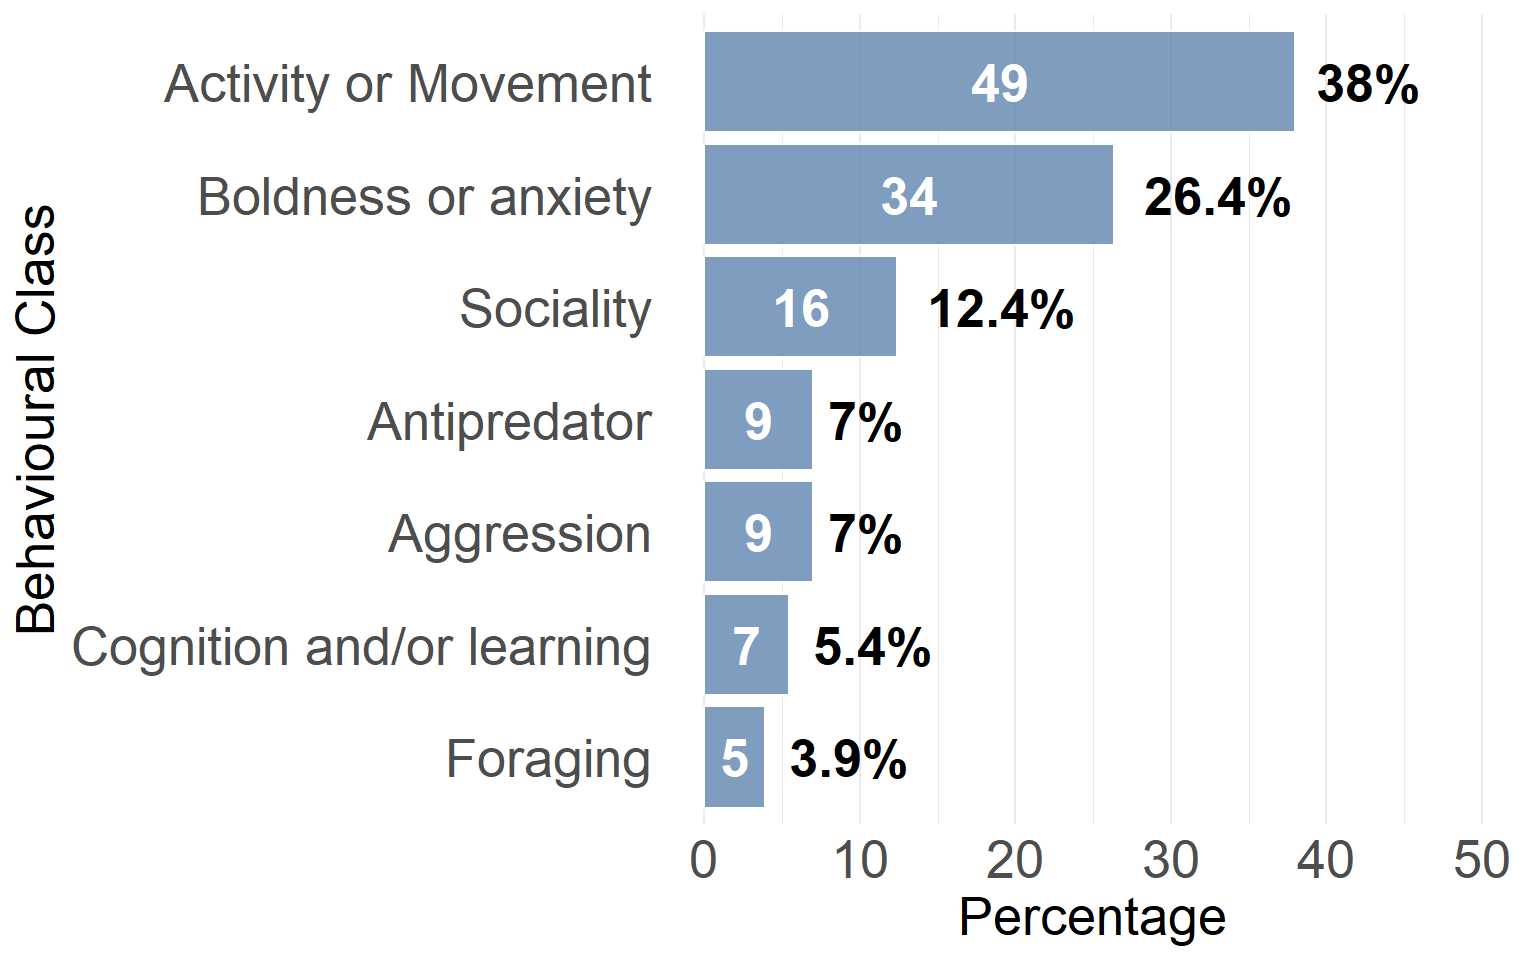
\includegraphics{zf_sm_code_files/figure-latex/unnamed-chunk-23-1.pdf}

\hypertarget{figs15---total-number-of-studies-investigating-each-behavioural-assay-of-behavioural_foraging}{%
\subsection{figs15 - total number of studies investigating each
behavioural assay of
behavioural\_foraging}\label{figs15---total-number-of-studies-investigating-each-behavioural-assay-of-behavioural_foraging}}

\begin{Shaded}
\begin{Highlighting}[]
\CommentTok{\# Calculate count for each assay in foraging behavior}
\NormalTok{total\_behaviour\_foraging\_count }\OtherTok{\textless{}{-}}\NormalTok{ bd }\SpecialCharTok{\%\textgreater{}\%} 
  \FunctionTok{separate\_rows}\NormalTok{(behaviour\_foraging, }\AttributeTok{sep =} \StringTok{",}\SpecialCharTok{\textbackslash{}\textbackslash{}}\StringTok{s*"}\NormalTok{) }\SpecialCharTok{\%\textgreater{}\%}  
  \FunctionTok{count}\NormalTok{(behaviour\_foraging) }\SpecialCharTok{\%\textgreater{}\%} 
  \FunctionTok{na.omit}\NormalTok{()}

\CommentTok{\# Calculate proportion and percentage for each category}
\NormalTok{behav\_foraging\_pct }\OtherTok{\textless{}{-}}\NormalTok{ total\_behaviour\_foraging\_count }\SpecialCharTok{\%\textgreater{}\%}
  \FunctionTok{mutate}\NormalTok{(}\AttributeTok{proportion =}\NormalTok{ n}\SpecialCharTok{/}\FunctionTok{sum}\NormalTok{(total\_behaviour\_foraging\_count}\SpecialCharTok{$}\NormalTok{n),}
         \AttributeTok{percentage =}\NormalTok{ proportion}\SpecialCharTok{*}\DecValTok{100}\NormalTok{)}

\CommentTok{\# Create a bar chart with the count on the x{-}axis and foraging behavior assay on the y{-}axis}
\NormalTok{figs15 }\OtherTok{\textless{}{-}}  \FunctionTok{ggplot}\NormalTok{(behav\_foraging\_pct, }\FunctionTok{aes}\NormalTok{(}\AttributeTok{x =} \FunctionTok{reorder}\NormalTok{(behaviour\_foraging, n), }\AttributeTok{y =}\NormalTok{ percentage)) }\SpecialCharTok{+}
  
  \CommentTok{\# Customize the appearance of the bars }
  \FunctionTok{geom\_bar}\NormalTok{(}\AttributeTok{stat =} \StringTok{"identity"}\NormalTok{, }\AttributeTok{fill =} \StringTok{"\#5F85AE"}\NormalTok{, }\AttributeTok{color =} \StringTok{"white"}\NormalTok{, }\AttributeTok{alpha =} \FloatTok{0.8}\NormalTok{, }\AttributeTok{position =} \FunctionTok{position\_dodge}\NormalTok{(}\FloatTok{0.9}\NormalTok{)) }\SpecialCharTok{+}
  
 \CommentTok{\# Add labels to the bars for percentage }
  \FunctionTok{geom\_text}\NormalTok{(}\FunctionTok{aes}\NormalTok{(}\AttributeTok{label =} \FunctionTok{paste0}\NormalTok{(}\FunctionTok{round}\NormalTok{(percentage, }\DecValTok{1}\NormalTok{), }\StringTok{"\%"}\NormalTok{)), }\AttributeTok{hjust =} \SpecialCharTok{{-}}\FloatTok{0.2}\NormalTok{, }\AttributeTok{vjust =} \FloatTok{0.5}\NormalTok{, }\AttributeTok{size =} \DecValTok{5}\NormalTok{, }\AttributeTok{fontface =} \StringTok{"bold"}\NormalTok{,     }\AttributeTok{color =} \StringTok{"black"}\NormalTok{) }\SpecialCharTok{+}
    
  \CommentTok{\# Add labels to the bars for absolute count  }
  \FunctionTok{geom\_text}\NormalTok{(}\FunctionTok{aes}\NormalTok{(}\AttributeTok{label =}\NormalTok{ n), }\AttributeTok{position =} \FunctionTok{position\_stack}\NormalTok{(}\AttributeTok{vjust =} \FloatTok{0.5}\NormalTok{), }\AttributeTok{color =} \StringTok{"white"}\NormalTok{, }\AttributeTok{size =} \DecValTok{5}\NormalTok{, }\AttributeTok{hjust =} \FloatTok{0.5}\NormalTok{, }\AttributeTok{fontface =}   \StringTok{"bold"}\NormalTok{) }\SpecialCharTok{+}
  
  \CommentTok{\# Add axis and plot labels}
  \FunctionTok{labs}\NormalTok{(}\AttributeTok{x =} \StringTok{"Foraging Behavior Assay"}\NormalTok{, }\AttributeTok{y =} \StringTok{"Percentage"}\NormalTok{) }\SpecialCharTok{+}
  
  \CommentTok{\# Customize the plot theme}
  \FunctionTok{theme\_minimal}\NormalTok{() }\SpecialCharTok{+}
  \FunctionTok{theme}\NormalTok{(}\AttributeTok{panel.grid.major.y =} \FunctionTok{element\_blank}\NormalTok{(),}
    \AttributeTok{axis.line.y =} \FunctionTok{element\_blank}\NormalTok{(),}
    \AttributeTok{axis.ticks.y =} \FunctionTok{element\_blank}\NormalTok{(),}
    \AttributeTok{axis.text.x =} \FunctionTok{element\_text}\NormalTok{(}\AttributeTok{size =} \DecValTok{15}\NormalTok{),}
    \AttributeTok{axis.text.y =} \FunctionTok{element\_text}\NormalTok{(}\AttributeTok{size =} \DecValTok{15}\NormalTok{, }\AttributeTok{hjust =} \DecValTok{1}\NormalTok{),}
    \AttributeTok{axis.title.x =} \FunctionTok{element\_text}\NormalTok{(}\AttributeTok{size =} \DecValTok{15}\NormalTok{),}
    \AttributeTok{axis.title.y =} \FunctionTok{element\_text}\NormalTok{(}\AttributeTok{size =} \DecValTok{15}\NormalTok{),}
    \AttributeTok{plot.title =} \FunctionTok{element\_blank}\NormalTok{()) }\SpecialCharTok{+}
    \FunctionTok{coord\_flip}\NormalTok{() }\SpecialCharTok{+}
    \FunctionTok{ylim}\NormalTok{(}\DecValTok{0}\NormalTok{, }\DecValTok{100}\NormalTok{)}

\NormalTok{figs15}
\end{Highlighting}
\end{Shaded}

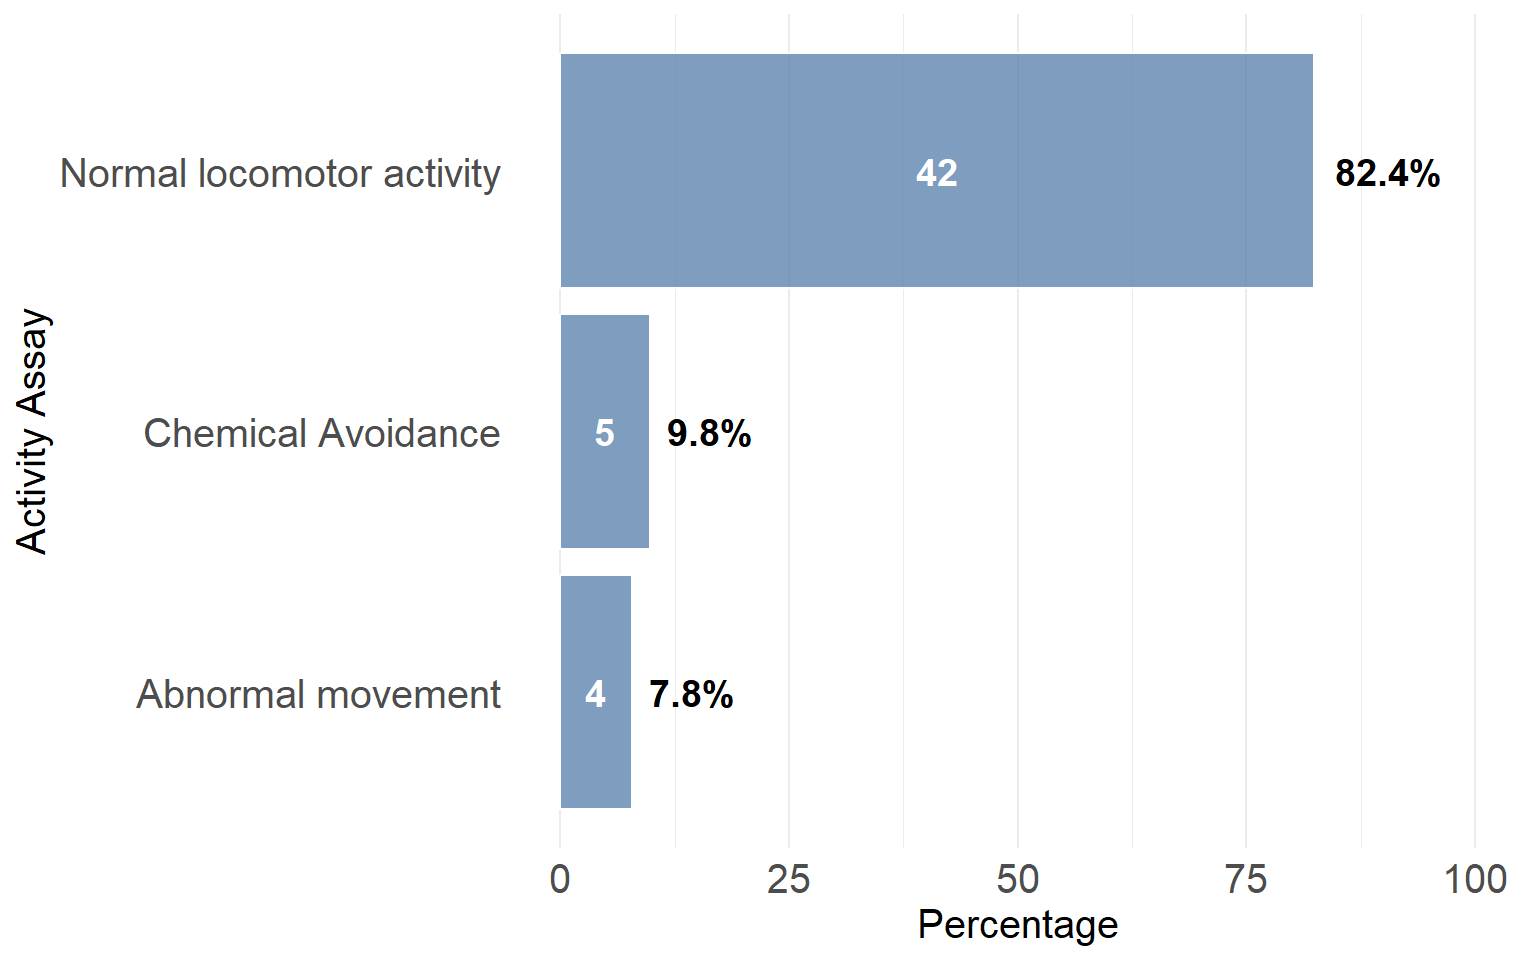
\includegraphics{zf_sm_code_files/figure-latex/unnamed-chunk-24-1.pdf}

\hypertarget{figs16---total-number-of-studies-investigating-each-behavioural-assay-of-anti-predator-behaviour}{%
\subsection{figs16 - total number of studies investigating each
behavioural assay of anti-predator
behaviour}\label{figs16---total-number-of-studies-investigating-each-behavioural-assay-of-anti-predator-behaviour}}

\begin{Shaded}
\begin{Highlighting}[]
\CommentTok{\# Calculate count for each assay in antipredator behavior}
\NormalTok{total\_behaviour\_antipredator\_count }\OtherTok{\textless{}{-}}\NormalTok{ bd }\SpecialCharTok{\%\textgreater{}\%} 
  \FunctionTok{separate\_rows}\NormalTok{(behaviour\_antipredator, }\AttributeTok{sep =} \StringTok{",}\SpecialCharTok{\textbackslash{}\textbackslash{}}\StringTok{s*"}\NormalTok{) }\SpecialCharTok{\%\textgreater{}\%}  
  \FunctionTok{count}\NormalTok{(behaviour\_antipredator) }\SpecialCharTok{\%\textgreater{}\%} 
  \FunctionTok{na.omit}\NormalTok{()}

\CommentTok{\# Calculate proportion and percentage for each category}
\NormalTok{behav\_antipredator\_pct }\OtherTok{\textless{}{-}}\NormalTok{ total\_behaviour\_antipredator\_count }\SpecialCharTok{\%\textgreater{}\%}
  \FunctionTok{mutate}\NormalTok{(}\AttributeTok{proportion =}\NormalTok{ n}\SpecialCharTok{/}\FunctionTok{sum}\NormalTok{(total\_behaviour\_antipredator\_count}\SpecialCharTok{$}\NormalTok{n),}
         \AttributeTok{percentage =}\NormalTok{ proportion}\SpecialCharTok{*}\DecValTok{100}\NormalTok{)}

\CommentTok{\# Create a bar chart with the count on the x{-}axis and antipredator behavior assay on the y{-}axis}
\NormalTok{figs16 }\OtherTok{\textless{}{-}} \FunctionTok{ggplot}\NormalTok{(behav\_antipredator\_pct, }\FunctionTok{aes}\NormalTok{(}\AttributeTok{x =} \FunctionTok{reorder}\NormalTok{(behaviour\_antipredator, n), }\AttributeTok{y =}\NormalTok{ percentage)) }\SpecialCharTok{+}
  
  \CommentTok{\# Customize the appearance of the bars }
  \FunctionTok{geom\_bar}\NormalTok{(}\AttributeTok{stat =} \StringTok{"identity"}\NormalTok{, }\AttributeTok{fill =} \StringTok{"\#5F85AE"}\NormalTok{, }\AttributeTok{color =} \StringTok{"white"}\NormalTok{, }\AttributeTok{alpha =} \FloatTok{0.8}\NormalTok{, }\AttributeTok{position =} \FunctionTok{position\_dodge}\NormalTok{(}\FloatTok{0.9}\NormalTok{)) }\SpecialCharTok{+}
  
  \CommentTok{\# Add labels to the bars for percentage }
  \FunctionTok{geom\_text}\NormalTok{(}\FunctionTok{aes}\NormalTok{(}\AttributeTok{label =} \FunctionTok{paste0}\NormalTok{(}\FunctionTok{round}\NormalTok{(percentage, }\DecValTok{1}\NormalTok{), }\StringTok{"\%"}\NormalTok{)), }\AttributeTok{hjust =} \SpecialCharTok{{-}}\FloatTok{0.2}\NormalTok{, }\AttributeTok{vjust =} \FloatTok{0.5}\NormalTok{, }\AttributeTok{size =} \DecValTok{5}\NormalTok{, }\AttributeTok{fontface =} \StringTok{"bold"}\NormalTok{, }\AttributeTok{color =} \StringTok{"black"}\NormalTok{) }\SpecialCharTok{+}
    
  \CommentTok{\# Add labels to the bars for absolute count  }
  \FunctionTok{geom\_text}\NormalTok{(}\FunctionTok{aes}\NormalTok{(}\AttributeTok{label =}\NormalTok{ n), }\AttributeTok{position =} \FunctionTok{position\_stack}\NormalTok{(}\AttributeTok{vjust =} \FloatTok{0.5}\NormalTok{), }\AttributeTok{color =} \StringTok{"white"}\NormalTok{, }\AttributeTok{size =} \DecValTok{5}\NormalTok{, }\AttributeTok{hjust =} \FloatTok{0.5}\NormalTok{, }\AttributeTok{fontface =} \StringTok{"bold"}\NormalTok{) }\SpecialCharTok{+}
  
  \CommentTok{\# Add axis and plot labels}
  \FunctionTok{labs}\NormalTok{(}\AttributeTok{x =} \StringTok{"Antipredator Behavior Assay"}\NormalTok{, }\AttributeTok{y =} \StringTok{"Percentage"}\NormalTok{) }\SpecialCharTok{+}
  
  \CommentTok{\# Customize the plot theme}
  \FunctionTok{theme\_minimal}\NormalTok{() }\SpecialCharTok{+}
  \FunctionTok{theme}\NormalTok{(}\AttributeTok{panel.grid.major.y =} \FunctionTok{element\_blank}\NormalTok{(),}
        \AttributeTok{axis.line.y =} \FunctionTok{element\_blank}\NormalTok{(),}
        \AttributeTok{axis.ticks.y =} \FunctionTok{element\_blank}\NormalTok{(),}
        \AttributeTok{axis.text.x =} \FunctionTok{element\_text}\NormalTok{(}\AttributeTok{size =} \DecValTok{15}\NormalTok{),}
        \AttributeTok{axis.text.y =} \FunctionTok{element\_text}\NormalTok{(}\AttributeTok{size =} \DecValTok{15}\NormalTok{, }\AttributeTok{hjust =} \DecValTok{1}\NormalTok{),}
        \AttributeTok{axis.title.x =} \FunctionTok{element\_text}\NormalTok{(}\AttributeTok{size =} \DecValTok{15}\NormalTok{),}
        \AttributeTok{axis.title.y =} \FunctionTok{element\_text}\NormalTok{(}\AttributeTok{size =} \DecValTok{15}\NormalTok{),}
        \AttributeTok{plot.title =} \FunctionTok{element\_blank}\NormalTok{()) }\SpecialCharTok{+}
  \FunctionTok{coord\_flip}\NormalTok{() }\SpecialCharTok{+}
  \FunctionTok{ylim}\NormalTok{(}\DecValTok{0}\NormalTok{, }\DecValTok{100}\NormalTok{)}

\NormalTok{figs16}
\end{Highlighting}
\end{Shaded}

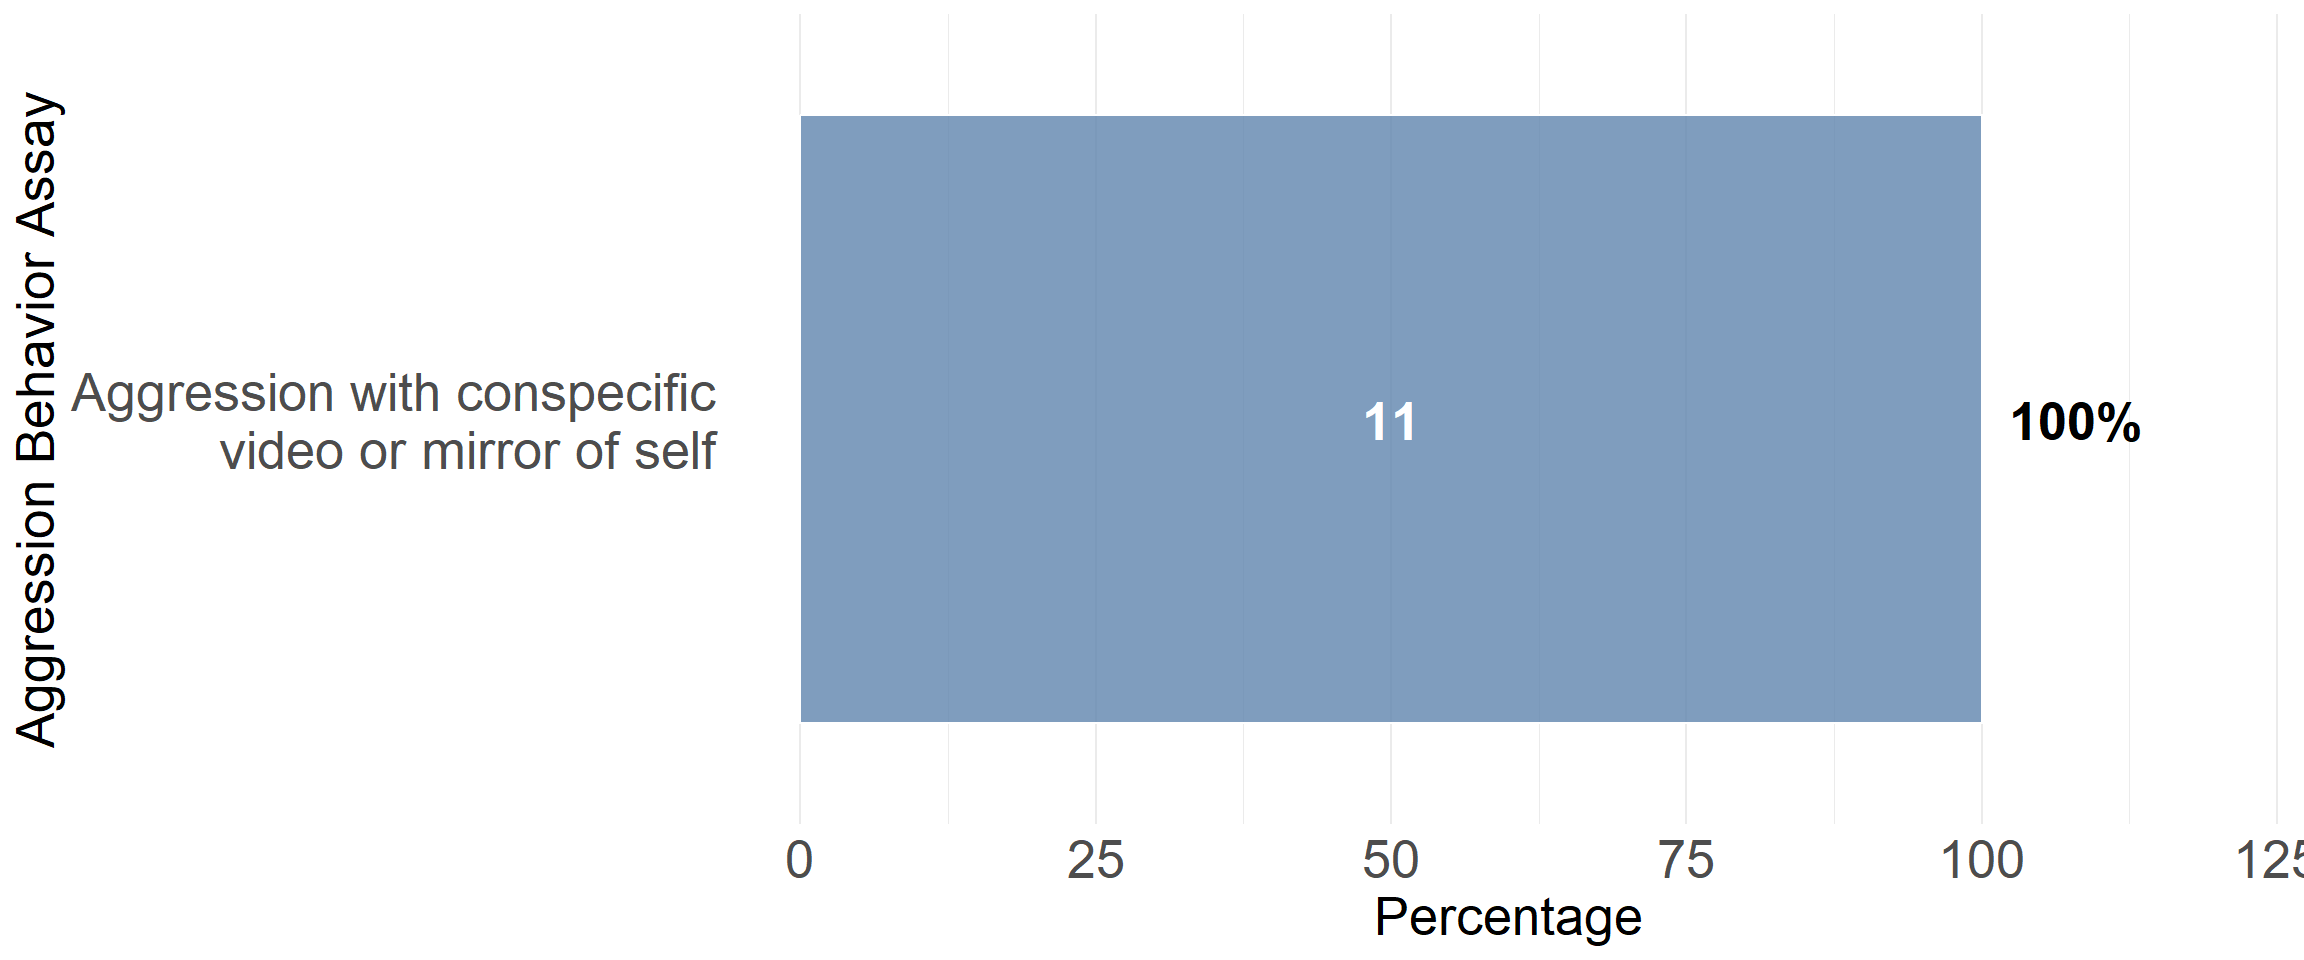
\includegraphics{zf_sm_code_files/figure-latex/unnamed-chunk-25-1.pdf}

\hypertarget{figs17---total-number-of-studies-investigating-each-behavioural-assay-of-anxiety-or-boldness-behaviour}{%
\subsection{figs17 - total number of studies investigating each
behavioural assay of Anxiety or Boldness
behaviour}\label{figs17---total-number-of-studies-investigating-each-behavioural-assay-of-anxiety-or-boldness-behaviour}}

\begin{Shaded}
\begin{Highlighting}[]
\CommentTok{\# Calculate count for each assay in anxiety behavior}
\NormalTok{total\_behaviour\_anxiety\_count }\OtherTok{\textless{}{-}}\NormalTok{ bd }\SpecialCharTok{\%\textgreater{}\%} 
  \FunctionTok{separate\_rows}\NormalTok{(behaviour\_anxiety, }\AttributeTok{sep =} \StringTok{",}\SpecialCharTok{\textbackslash{}\textbackslash{}}\StringTok{s*"}\NormalTok{) }\SpecialCharTok{\%\textgreater{}\%}  
  \FunctionTok{count}\NormalTok{(behaviour\_anxiety) }\SpecialCharTok{\%\textgreater{}\%} 
  \FunctionTok{na.omit}\NormalTok{()}

\CommentTok{\# Calculate proportion and percentage for each category}
\NormalTok{behav\_anxiety\_pct }\OtherTok{\textless{}{-}}\NormalTok{ total\_behaviour\_anxiety\_count }\SpecialCharTok{\%\textgreater{}\%}
  \FunctionTok{mutate}\NormalTok{(}\AttributeTok{proportion =}\NormalTok{ n}\SpecialCharTok{/}\FunctionTok{sum}\NormalTok{(total\_behaviour\_anxiety\_count}\SpecialCharTok{$}\NormalTok{n),}
         \AttributeTok{percentage =}\NormalTok{ proportion}\SpecialCharTok{*}\DecValTok{100}\NormalTok{)}

\CommentTok{\# Create a bar chart with the count on the x{-}axis and anxiety behavior assay on the y{-}axis}
\NormalTok{figs17 }\OtherTok{\textless{}{-}} \FunctionTok{ggplot}\NormalTok{(behav\_anxiety\_pct, }\FunctionTok{aes}\NormalTok{(}\AttributeTok{x =} \FunctionTok{reorder}\NormalTok{(behaviour\_anxiety, n), }\AttributeTok{y =}\NormalTok{ percentage)) }\SpecialCharTok{+}
  
  \CommentTok{\# Customize the appearance of the bars }
  \FunctionTok{geom\_bar}\NormalTok{(}\AttributeTok{stat =} \StringTok{"identity"}\NormalTok{, }\AttributeTok{fill =} \StringTok{"\#5F85AE"}\NormalTok{, }\AttributeTok{color =} \StringTok{"white"}\NormalTok{, }\AttributeTok{alpha =} \FloatTok{0.8}\NormalTok{, }\AttributeTok{position =} \FunctionTok{position\_dodge}\NormalTok{(}\FloatTok{0.9}\NormalTok{)) }\SpecialCharTok{+}
  
  \CommentTok{\# Add labels to the bars for percentage }
  \FunctionTok{geom\_text}\NormalTok{(}\FunctionTok{aes}\NormalTok{(}\AttributeTok{label =} \FunctionTok{paste0}\NormalTok{(}\FunctionTok{round}\NormalTok{(percentage, }\DecValTok{1}\NormalTok{), }\StringTok{"\%"}\NormalTok{)), }\AttributeTok{hjust =} \SpecialCharTok{{-}}\FloatTok{0.2}\NormalTok{, }\AttributeTok{vjust =} \FloatTok{0.5}\NormalTok{, }\AttributeTok{size =} \DecValTok{5}\NormalTok{, }\AttributeTok{fontface =} \StringTok{"bold"}\NormalTok{, }\AttributeTok{color =} \StringTok{"black"}\NormalTok{) }\SpecialCharTok{+}
    
  \CommentTok{\# Add labels to the bars for absolute count  }
  \FunctionTok{geom\_text}\NormalTok{(}\FunctionTok{aes}\NormalTok{(}\AttributeTok{label =}\NormalTok{ n), }\AttributeTok{position =} \FunctionTok{position\_stack}\NormalTok{(}\AttributeTok{vjust =} \FloatTok{0.5}\NormalTok{), }\AttributeTok{color =} \StringTok{"white"}\NormalTok{, }\AttributeTok{size =} \DecValTok{5}\NormalTok{, }\AttributeTok{hjust =} \FloatTok{0.5}\NormalTok{, }\AttributeTok{fontface =} \StringTok{"bold"}\NormalTok{) }\SpecialCharTok{+}
  
  \CommentTok{\# Add axis and plot labels}
  \FunctionTok{labs}\NormalTok{(}\AttributeTok{x =} \StringTok{"Anxiety Behavior Assay"}\NormalTok{, }\AttributeTok{y =} \StringTok{"Percentage"}\NormalTok{) }\SpecialCharTok{+}
  
  \CommentTok{\# Customize the plot theme}
  \FunctionTok{theme\_minimal}\NormalTok{() }\SpecialCharTok{+}
  \FunctionTok{theme}\NormalTok{(}\AttributeTok{panel.grid.major.y =} \FunctionTok{element\_blank}\NormalTok{(),}
        \AttributeTok{axis.line.y =} \FunctionTok{element\_blank}\NormalTok{(),}
        \AttributeTok{axis.ticks.y =} \FunctionTok{element\_blank}\NormalTok{(),}
        \AttributeTok{axis.text.x =} \FunctionTok{element\_text}\NormalTok{(}\AttributeTok{size =} \DecValTok{15}\NormalTok{),}
        \AttributeTok{axis.text.y =} \FunctionTok{element\_text}\NormalTok{(}\AttributeTok{size =} \DecValTok{15}\NormalTok{, }\AttributeTok{hjust =} \DecValTok{1}\NormalTok{),}
        \AttributeTok{axis.title.x =} \FunctionTok{element\_text}\NormalTok{(}\AttributeTok{size =} \DecValTok{15}\NormalTok{),}
        \AttributeTok{axis.title.y =} \FunctionTok{element\_text}\NormalTok{(}\AttributeTok{size =} \DecValTok{15}\NormalTok{),}
        \AttributeTok{plot.title =} \FunctionTok{element\_blank}\NormalTok{()) }\SpecialCharTok{+}
        \FunctionTok{coord\_flip}\NormalTok{() }\SpecialCharTok{+}
        \FunctionTok{ylim}\NormalTok{(}\DecValTok{0}\NormalTok{, }\DecValTok{80}\NormalTok{)}

\NormalTok{figs17}
\end{Highlighting}
\end{Shaded}

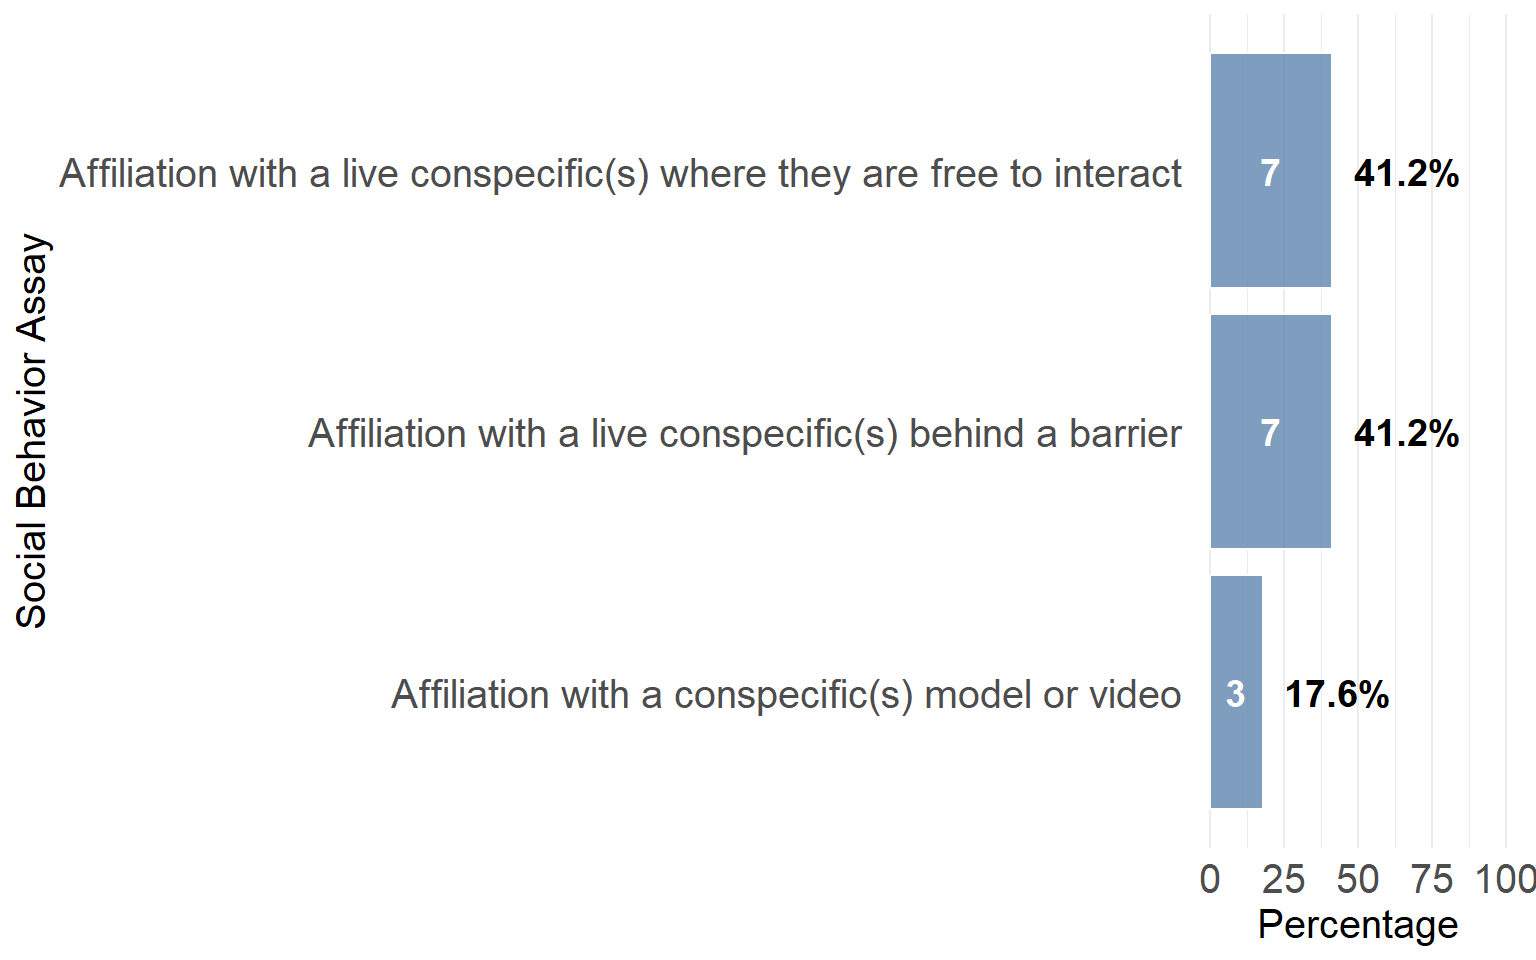
\includegraphics{zf_sm_code_files/figure-latex/unnamed-chunk-26-1.pdf}

\hypertarget{figs18---heat-map-to-show-which-behavours-have-been-investigated-in-which-pesticide-target-class}{%
\subsection{figs18 - heat map to show which behavours have been
investigated in which pesticide target
class}\label{figs18---heat-map-to-show-which-behavours-have-been-investigated-in-which-pesticide-target-class}}

\begin{Shaded}
\begin{Highlighting}[]
\CommentTok{\# Join the behaviour details and pesticide details by "study\_id"}
\NormalTok{bd\_pd }\OtherTok{\textless{}{-}} \FunctionTok{left\_join}\NormalTok{(bd, pd, }\AttributeTok{by =} \StringTok{"study\_id"}\NormalTok{)}

\CommentTok{\# Separate rows in "bd\_pd" by "behavioural\_class" and "pesticide\_target\_class" columns}
\NormalTok{bd\_pd1 }\OtherTok{\textless{}{-}} \FunctionTok{separate\_rows}\NormalTok{(bd\_pd, behavioural\_class, }\AttributeTok{sep =} \StringTok{",}\SpecialCharTok{\textbackslash{}\textbackslash{}}\StringTok{s*"}\NormalTok{, }\AttributeTok{convert =} \ConstantTok{TRUE}\NormalTok{)}
\NormalTok{bd\_pd1}\OtherTok{\textless{}{-}} \FunctionTok{separate\_rows}\NormalTok{(bd\_pd1, pesticide\_target\_class, }\AttributeTok{sep =} \StringTok{",}\SpecialCharTok{\textbackslash{}\textbackslash{}}\StringTok{s*"}\NormalTok{, }\AttributeTok{convert =} \ConstantTok{TRUE}\NormalTok{)}

\CommentTok{\# Group by "behavioural\_class" and "pesticide\_target\_class" and summarize count}
\NormalTok{bd\_pd\_summary1 }\OtherTok{\textless{}{-}}\NormalTok{ bd\_pd1 }\SpecialCharTok{\%\textgreater{}\%}
  \FunctionTok{mutate}\NormalTok{(}\AttributeTok{behavioural\_class =} \FunctionTok{str\_trim}\NormalTok{(behavioural\_class),}
         \AttributeTok{pesticide\_target\_class =} \FunctionTok{str\_trim}\NormalTok{(pesticide\_target\_class)) }\SpecialCharTok{\%\textgreater{}\%}
  \FunctionTok{group\_by}\NormalTok{(behavioural\_class, pesticide\_target\_class) }\SpecialCharTok{\%\textgreater{}\%}
  \FunctionTok{summarise}\NormalTok{(}\AttributeTok{count =} \FunctionTok{n}\NormalTok{()) }\SpecialCharTok{\%\textgreater{}\%}
  \FunctionTok{ungroup}\NormalTok{() }
\end{Highlighting}
\end{Shaded}

\begin{verbatim}
## `summarise()` has grouped output by 'behavioural_class'. You can override using
## the `.groups` argument.
\end{verbatim}

\begin{Shaded}
\begin{Highlighting}[]
\CommentTok{\# Create a heatmap with pesticide target class on the x{-}axis and behavioural class on the y{-}axis}
\NormalTok{figs18 }\OtherTok{\textless{}{-}} \FunctionTok{ggplot}\NormalTok{(bd\_pd\_summary1, }\FunctionTok{aes}\NormalTok{(}\AttributeTok{x =}\NormalTok{ pesticide\_target\_class, }\AttributeTok{y =}\NormalTok{ behavioural\_class, }\AttributeTok{fill =}\NormalTok{ count)) }\SpecialCharTok{+}
  
  \CommentTok{\#Create and fill each tile }
  \FunctionTok{geom\_tile}\NormalTok{(}\AttributeTok{color =} \StringTok{"white"}\NormalTok{) }\SpecialCharTok{+}
  \FunctionTok{scale\_fill\_gradient}\NormalTok{(}\AttributeTok{low =} \StringTok{"\#F0F4F8"}\NormalTok{, }\AttributeTok{high =} \StringTok{"\#446487"}\NormalTok{) }\SpecialCharTok{+}
  
  \CommentTok{\# Add labels to the bars for absolute count  }
  \FunctionTok{geom\_text}\NormalTok{(}\FunctionTok{aes}\NormalTok{(}\AttributeTok{label =}\NormalTok{ count), }\AttributeTok{color =} \StringTok{"black"}\NormalTok{, }\AttributeTok{size =} \DecValTok{4}\NormalTok{) }\SpecialCharTok{+} 
  
  \CommentTok{\# Add axis and plot labels}
  \FunctionTok{labs}\NormalTok{(}\AttributeTok{x =} \StringTok{"Pesticide Target Class"}\NormalTok{, }\AttributeTok{y =} \StringTok{"Behavioural Class"}\NormalTok{, }\AttributeTok{fill =} \StringTok{"Count"}\NormalTok{) }\SpecialCharTok{+}
  
  \CommentTok{\# Customize the plot theme}
  \FunctionTok{theme\_minimal}\NormalTok{() }\SpecialCharTok{+}
  \FunctionTok{theme}\NormalTok{(}\AttributeTok{panel.grid.major.y =} \FunctionTok{element\_blank}\NormalTok{(),}
        \AttributeTok{axis.line.y =} \FunctionTok{element\_blank}\NormalTok{(),}
        \AttributeTok{axis.ticks.y =} \FunctionTok{element\_blank}\NormalTok{(),}
        \AttributeTok{axis.text.x =} \FunctionTok{element\_text}\NormalTok{(}\AttributeTok{size =} \DecValTok{15}\NormalTok{),}
        \AttributeTok{axis.text.y =} \FunctionTok{element\_text}\NormalTok{(}\AttributeTok{size =} \DecValTok{15}\NormalTok{, }\AttributeTok{hjust =} \DecValTok{1}\NormalTok{),}
        \AttributeTok{axis.title.x =} \FunctionTok{element\_text}\NormalTok{(}\AttributeTok{size =} \DecValTok{15}\NormalTok{),}
        \AttributeTok{axis.title.y =} \FunctionTok{element\_text}\NormalTok{(}\AttributeTok{size =} \DecValTok{15}\NormalTok{),}
        \AttributeTok{plot.title =} \FunctionTok{element\_blank}\NormalTok{())}


\NormalTok{figs18}
\end{Highlighting}
\end{Shaded}

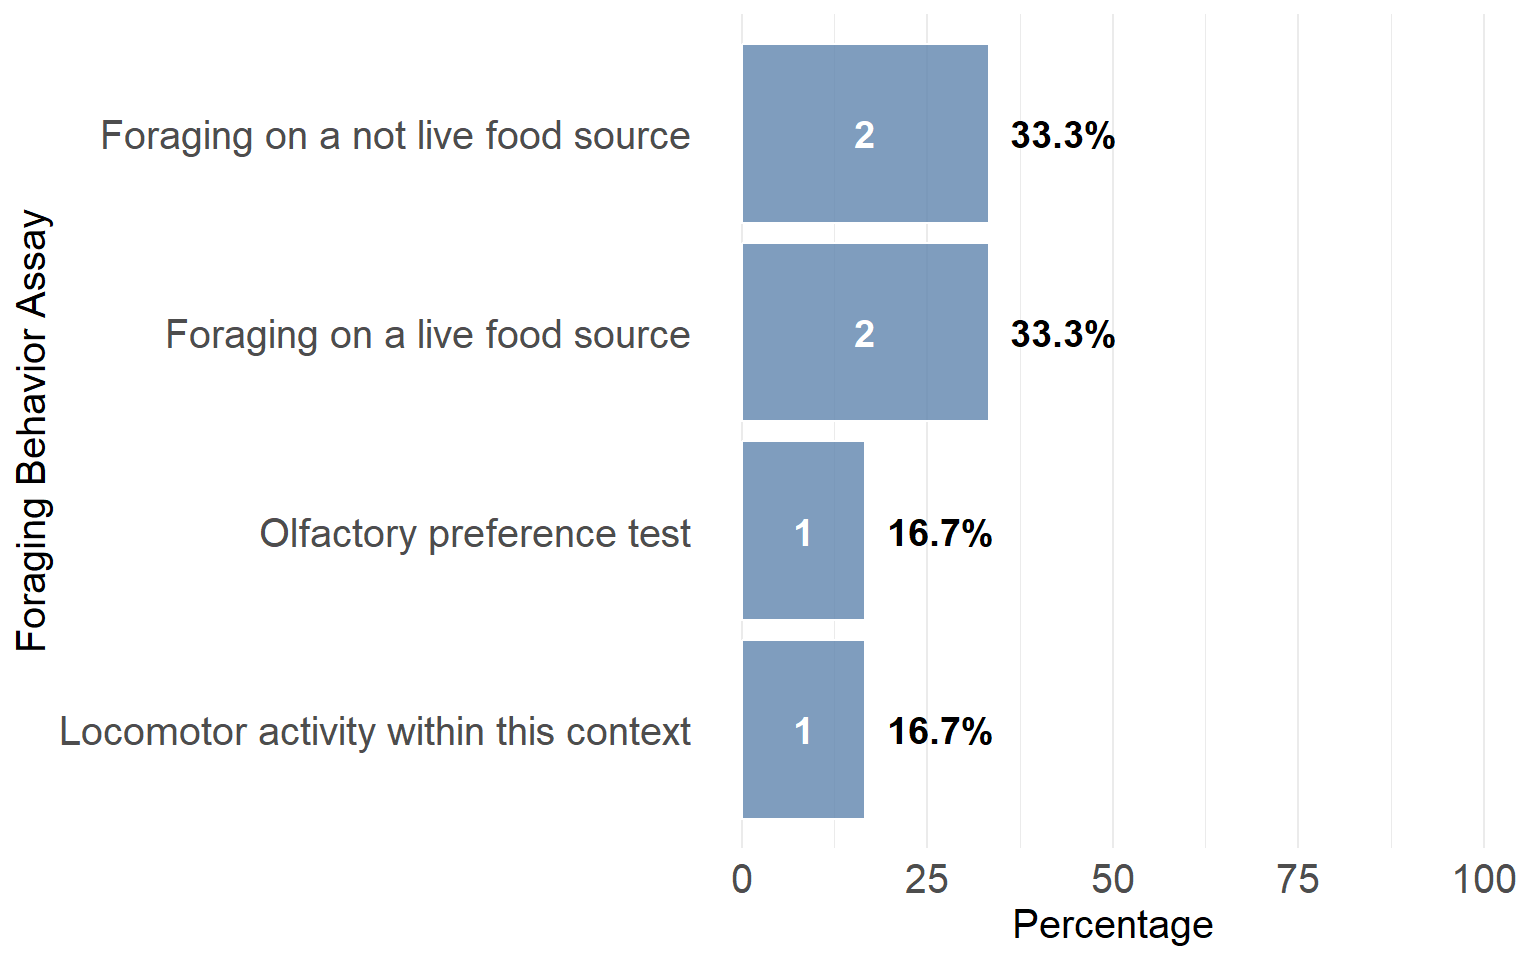
\includegraphics{zf_sm_code_files/figure-latex/unnamed-chunk-27-1.pdf}

\hypertarget{figs19---heat-map-to-show-which-behavours-have-been-investigated-in-which-pesticide-chemical-class}{%
\subsection{figs19 - heat map to show which behavours have been
investigated in which pesticide chemical
class}\label{figs19---heat-map-to-show-which-behavours-have-been-investigated-in-which-pesticide-chemical-class}}

\begin{Shaded}
\begin{Highlighting}[]
\CommentTok{\# Separate rows by behavioural\_class and pesticide\_chemical\_class columns}
\NormalTok{bd\_pd2 }\OtherTok{\textless{}{-}} \FunctionTok{separate\_rows}\NormalTok{(bd\_pd, behavioural\_class, }\AttributeTok{sep =} \StringTok{",}\SpecialCharTok{\textbackslash{}\textbackslash{}}\StringTok{s*"}\NormalTok{, }\AttributeTok{convert =} \ConstantTok{TRUE}\NormalTok{)}
\NormalTok{bd\_pd2 }\OtherTok{\textless{}{-}} \FunctionTok{separate\_rows}\NormalTok{(bd\_pd2, pesticide\_chemical\_class, }\AttributeTok{sep =} \StringTok{","}\NormalTok{, }\AttributeTok{convert =} \ConstantTok{TRUE}\NormalTok{)}

\CommentTok{\# Get the top 3 most numerous pesticide chemical classes}
\NormalTok{bd\_pd\_summary2 }\OtherTok{\textless{}{-}}\NormalTok{ bd\_pd2 }\SpecialCharTok{\%\textgreater{}\%}
  \FunctionTok{mutate}\NormalTok{(}\AttributeTok{behavioural\_class =} \FunctionTok{str\_trim}\NormalTok{(behavioural\_class),}
         \AttributeTok{pesticide\_target\_class =} \FunctionTok{str\_trim}\NormalTok{(pesticide\_chemical\_class)) }\SpecialCharTok{\%\textgreater{}\%}
  \FunctionTok{group\_by}\NormalTok{(behavioural\_class, pesticide\_chemical\_class) }\SpecialCharTok{\%\textgreater{}\%}
  \FunctionTok{summarise}\NormalTok{(}\AttributeTok{count =} \FunctionTok{n}\NormalTok{()) }\SpecialCharTok{\%\textgreater{}\%}
  \FunctionTok{ungroup}\NormalTok{() }
\end{Highlighting}
\end{Shaded}

\begin{verbatim}
## `summarise()` has grouped output by 'behavioural_class'. You can override using
## the `.groups` argument.
\end{verbatim}

\begin{Shaded}
\begin{Highlighting}[]
\NormalTok{top\_pesticide\_classes }\OtherTok{\textless{}{-}}\NormalTok{ bd\_pd\_summary2 }\SpecialCharTok{\%\textgreater{}\%}
  \FunctionTok{filter}\NormalTok{(}\SpecialCharTok{!}\FunctionTok{is.na}\NormalTok{(pesticide\_chemical\_class)) }\SpecialCharTok{\%\textgreater{}\%}
  \FunctionTok{group\_by}\NormalTok{(pesticide\_chemical\_class) }\SpecialCharTok{\%\textgreater{}\%}
  \FunctionTok{summarise}\NormalTok{(}\AttributeTok{count =} \FunctionTok{sum}\NormalTok{(count)) }\SpecialCharTok{\%\textgreater{}\%}
  \FunctionTok{ungroup}\NormalTok{() }\SpecialCharTok{\%\textgreater{}\%}
  \FunctionTok{top\_n}\NormalTok{(}\DecValTok{3}\NormalTok{, count) }\SpecialCharTok{\%\textgreater{}\%} 
  \FunctionTok{pull}\NormalTok{(pesticide\_chemical\_class)}

\CommentTok{\# Subset the data to include only the top 3 classes}
\NormalTok{bd\_pd\_summary\_top3 }\OtherTok{\textless{}{-}}\NormalTok{ bd\_pd\_summary2 }\SpecialCharTok{\%\textgreater{}\%}
  \FunctionTok{filter}\NormalTok{(pesticide\_chemical\_class }\SpecialCharTok{\%in\%}\NormalTok{ top\_pesticide\_classes)}

\CommentTok{\# Create a heatmap with pesticide chemical class on the x{-}axis and behavioral class on the y{-}axis}
\NormalTok{figs19 }\OtherTok{\textless{}{-}} \FunctionTok{ggplot}\NormalTok{(bd\_pd\_summary\_top3, }\FunctionTok{aes}\NormalTok{(}\AttributeTok{x =}\NormalTok{ pesticide\_chemical\_class, }\AttributeTok{y =}\NormalTok{ behavioural\_class, }\AttributeTok{fill =}\NormalTok{ count)) }\SpecialCharTok{+}
  
  \CommentTok{\#Create and fill each tile }
  \FunctionTok{geom\_tile}\NormalTok{(}\AttributeTok{color =} \StringTok{"white"}\NormalTok{) }\SpecialCharTok{+}
  \FunctionTok{scale\_fill\_gradient}\NormalTok{(}\AttributeTok{low =} \StringTok{"\#F0F4F8"}\NormalTok{, }\AttributeTok{high =} \StringTok{"\#446487"}\NormalTok{) }\SpecialCharTok{+}
  
  \CommentTok{\# Add labels to the bars for absolute count }
  \FunctionTok{geom\_text}\NormalTok{(}\FunctionTok{aes}\NormalTok{(}\AttributeTok{label =} \FunctionTok{ifelse}\NormalTok{(count }\SpecialCharTok{\textgreater{}} \DecValTok{0}\NormalTok{, count, }\StringTok{""}\NormalTok{)), }\AttributeTok{color =} \StringTok{"black"}\NormalTok{, }\AttributeTok{size =} \DecValTok{4}\NormalTok{) }\SpecialCharTok{+}  
  
  \CommentTok{\# Add axis and plot labels}
  \FunctionTok{labs}\NormalTok{(}\AttributeTok{x =} \StringTok{"Pesticide Chemical Class"}\NormalTok{, }\AttributeTok{y =} \StringTok{"Behavioural Class"}\NormalTok{, }\AttributeTok{fill =} \StringTok{"Count"}\NormalTok{) }\SpecialCharTok{+}
  
  \CommentTok{\# Customize the plot theme}
  \FunctionTok{theme\_minimal}\NormalTok{() }\SpecialCharTok{+}
  \FunctionTok{theme}\NormalTok{(}\AttributeTok{panel.grid.major.y =} \FunctionTok{element\_blank}\NormalTok{(),}
    \AttributeTok{axis.line.y =} \FunctionTok{element\_blank}\NormalTok{(),}
    \AttributeTok{axis.ticks.y =} \FunctionTok{element\_blank}\NormalTok{(),}
    \AttributeTok{axis.text.x =} \FunctionTok{element\_text}\NormalTok{(}\AttributeTok{size =} \DecValTok{15}\NormalTok{),}
    \AttributeTok{axis.text.y =} \FunctionTok{element\_text}\NormalTok{(}\AttributeTok{size =} \DecValTok{15}\NormalTok{, }\AttributeTok{hjust =} \DecValTok{1}\NormalTok{),}
    \AttributeTok{axis.title.x =} \FunctionTok{element\_text}\NormalTok{(}\AttributeTok{size =} \DecValTok{15}\NormalTok{),}
    \AttributeTok{axis.title.y =} \FunctionTok{element\_text}\NormalTok{(}\AttributeTok{size =} \DecValTok{15}\NormalTok{),}
    \AttributeTok{plot.title =} \FunctionTok{element\_blank}\NormalTok{())}
\NormalTok{figs19}
\end{Highlighting}
\end{Shaded}

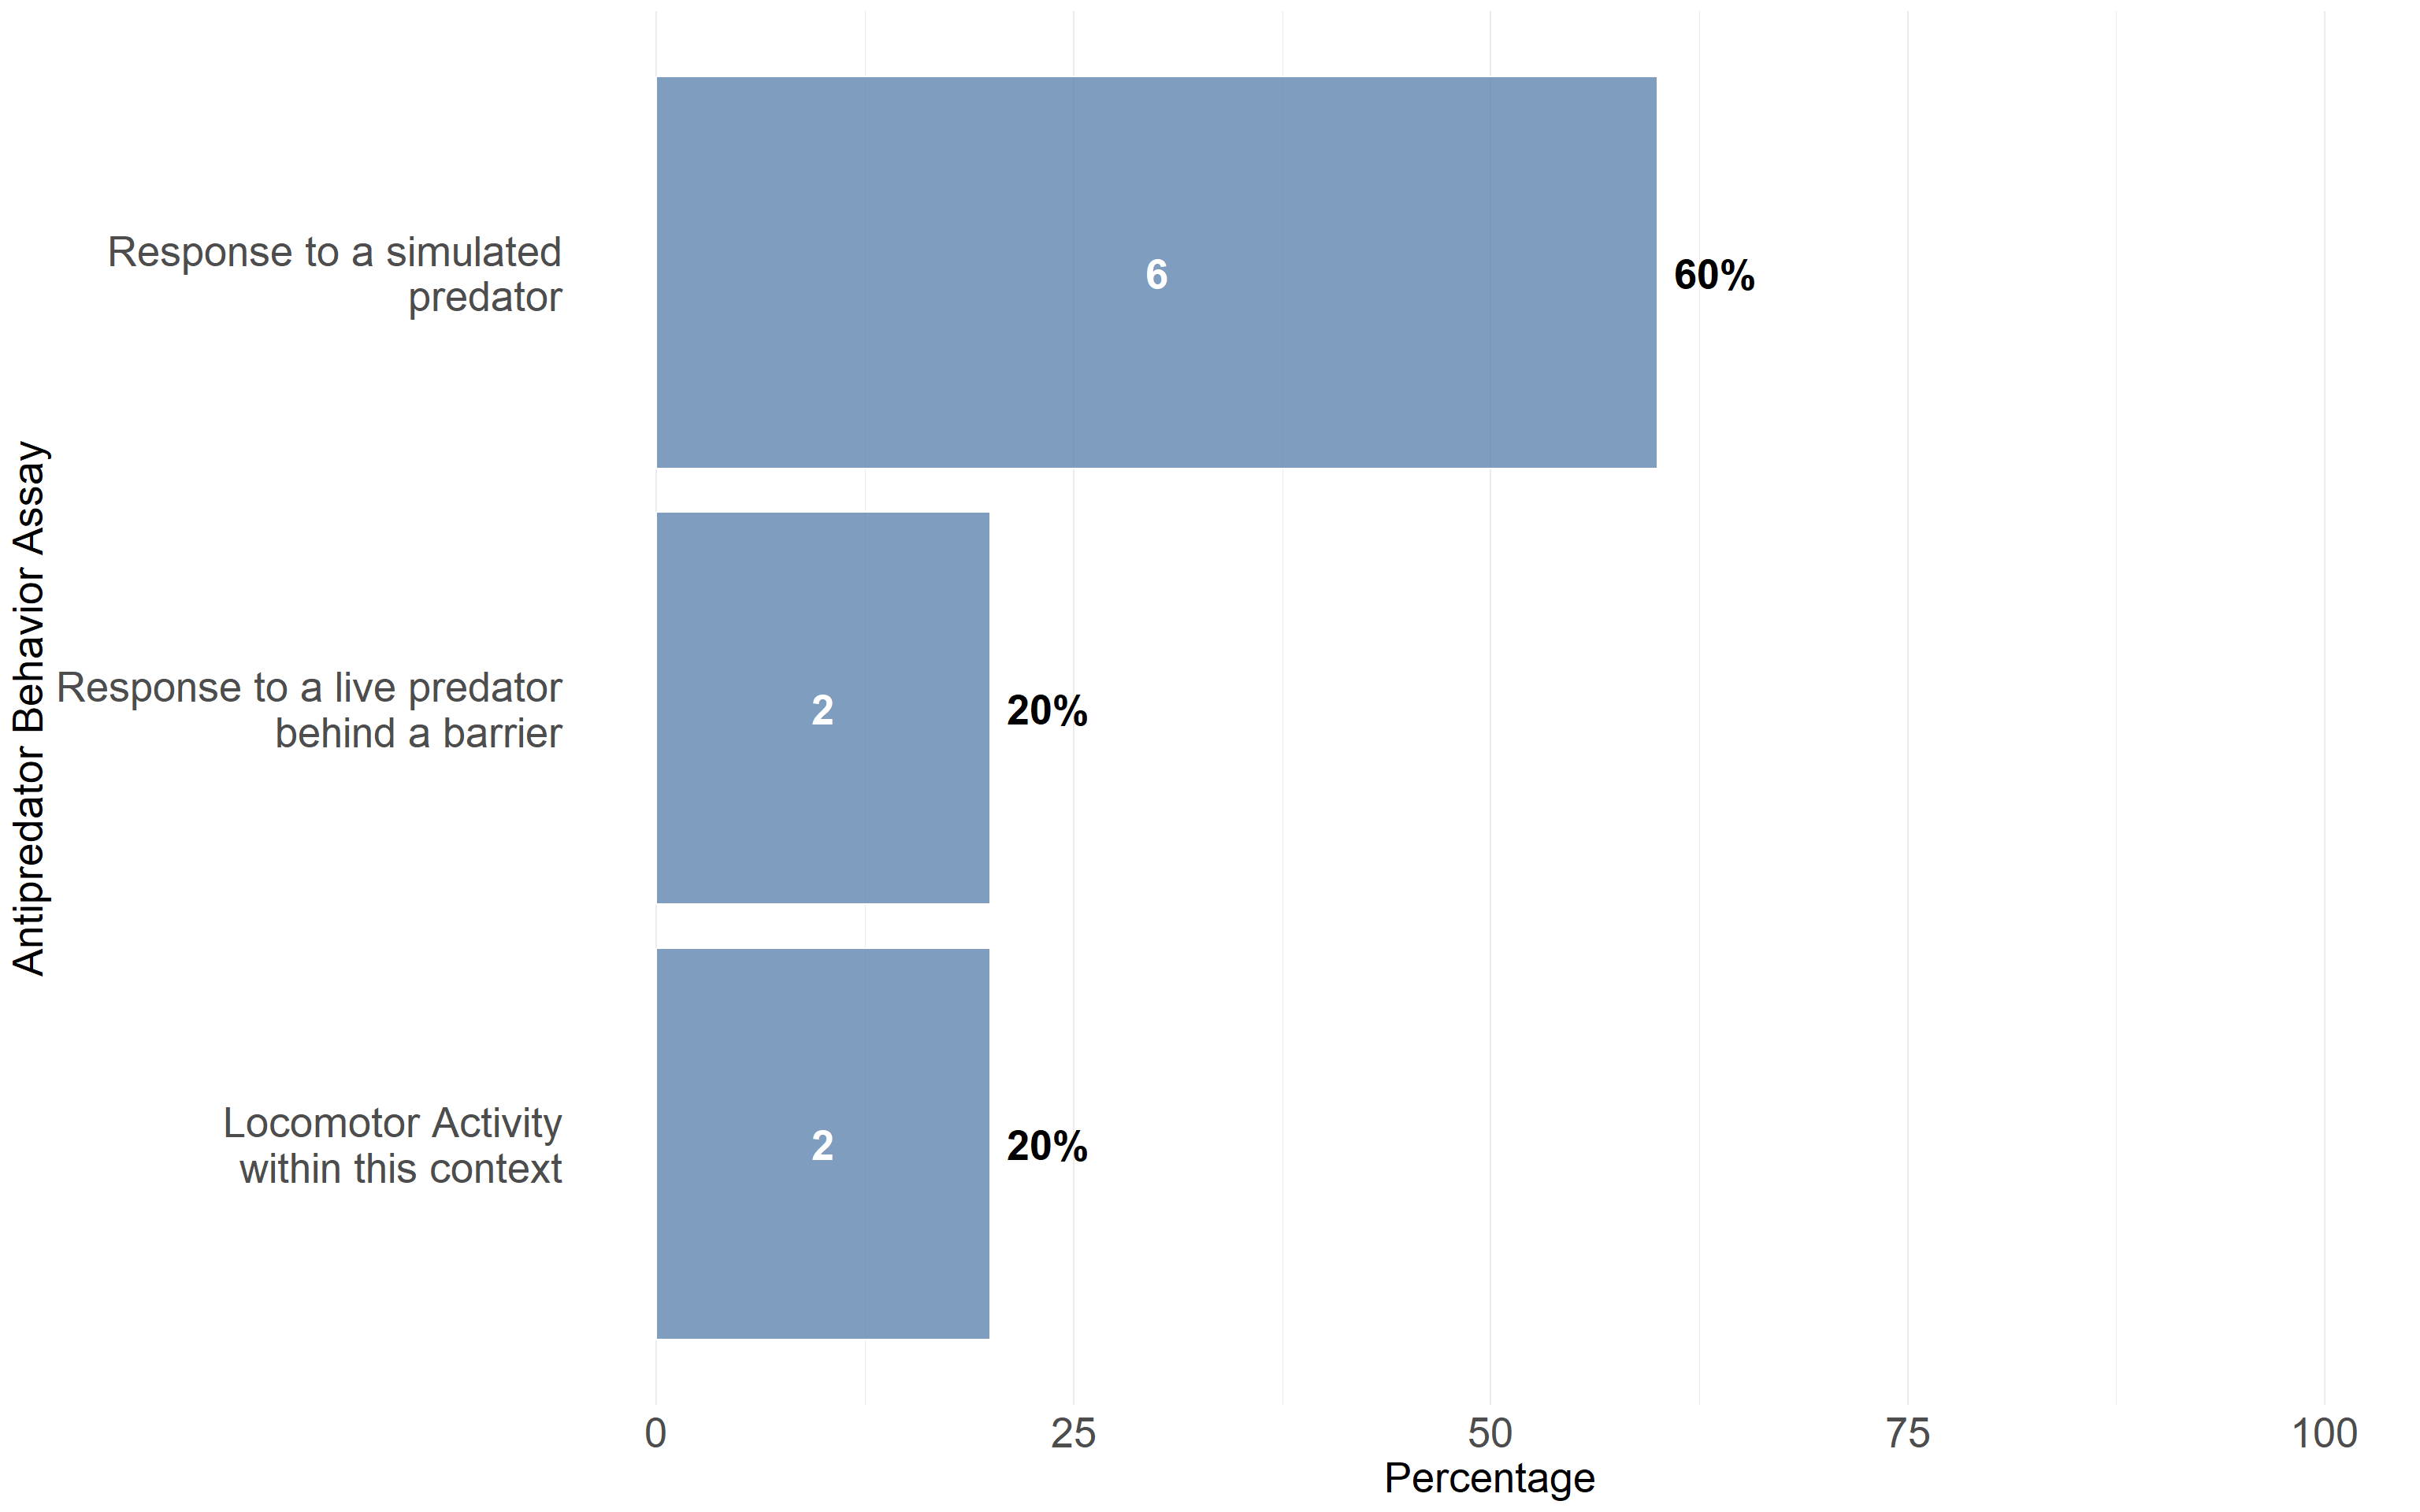
\includegraphics{zf_sm_code_files/figure-latex/unnamed-chunk-28-1.pdf}

\hypertarget{figs20---heat-map-to-show-which-life-stages-of-exposure-have-been-exposed-to-each-pesticide-chemical-class}{%
\subsection{figs20 - heat map to show which life stages of exposure have
been exposed to each pesticide chemical
class}\label{figs20---heat-map-to-show-which-life-stages-of-exposure-have-been-exposed-to-each-pesticide-chemical-class}}

\begin{Shaded}
\begin{Highlighting}[]
\CommentTok{\# Join the stydt details with pesticide details by "study\_id". }
\NormalTok{sd\_pd }\OtherTok{\textless{}{-}} \FunctionTok{left\_join}\NormalTok{(sd, pd, }\AttributeTok{by =} \StringTok{"study\_id"}\NormalTok{)}

\CommentTok{\# Separate rows in "sd\_pd" by "life\_stage\_exposure" and "pesticide\_chemical\_class" columns}
\NormalTok{sd\_pd1 }\OtherTok{\textless{}{-}} \FunctionTok{separate\_rows}\NormalTok{(sd\_pd, life\_stage\_exposure, }\AttributeTok{sep =} \StringTok{","}\NormalTok{, }\AttributeTok{convert =} \ConstantTok{TRUE}\NormalTok{)}
\NormalTok{sd\_pd1 }\OtherTok{\textless{}{-}} \FunctionTok{separate\_rows}\NormalTok{(sd\_pd1, pesticide\_chemical\_class, }\AttributeTok{sep =} \StringTok{","}\NormalTok{, }\AttributeTok{convert =} \ConstantTok{TRUE}\NormalTok{)}

\CommentTok{\# Group by "life\_stage\_exposure" and "pesticide\_chemical\_class" and summarize count}
\NormalTok{sd\_pd\_summary1 }\OtherTok{\textless{}{-}}\NormalTok{ sd\_pd1 }\SpecialCharTok{\%\textgreater{}\%}
  \FunctionTok{mutate}\NormalTok{(}\AttributeTok{life\_stage\_exposure =} \FunctionTok{str\_trim}\NormalTok{(life\_stage\_exposure),}
         \AttributeTok{pesticide\_chemical\_class =} \FunctionTok{str\_trim}\NormalTok{(pesticide\_chemical\_class)) }\SpecialCharTok{\%\textgreater{}\%}
  \FunctionTok{group\_by}\NormalTok{(life\_stage\_exposure, pesticide\_chemical\_class) }\SpecialCharTok{\%\textgreater{}\%}
  \FunctionTok{summarise}\NormalTok{(}\AttributeTok{count =} \FunctionTok{n}\NormalTok{()) }\SpecialCharTok{\%\textgreater{}\%}
  \FunctionTok{ungroup}\NormalTok{()}
\end{Highlighting}
\end{Shaded}

\begin{verbatim}
## `summarise()` has grouped output by 'life_stage_exposure'. You can override
## using the `.groups` argument.
\end{verbatim}

\begin{Shaded}
\begin{Highlighting}[]
\NormalTok{top\_pesticide\_classes }\OtherTok{\textless{}{-}}\NormalTok{ sd\_pd\_summary1 }\SpecialCharTok{\%\textgreater{}\%}
  \FunctionTok{filter}\NormalTok{(}\SpecialCharTok{!}\FunctionTok{is.na}\NormalTok{(pesticide\_chemical\_class)) }\SpecialCharTok{\%\textgreater{}\%}
  \FunctionTok{group\_by}\NormalTok{(pesticide\_chemical\_class) }\SpecialCharTok{\%\textgreater{}\%}
  \FunctionTok{summarise}\NormalTok{(}\AttributeTok{count =} \FunctionTok{sum}\NormalTok{(count)) }\SpecialCharTok{\%\textgreater{}\%}
  \FunctionTok{ungroup}\NormalTok{() }\SpecialCharTok{\%\textgreater{}\%}
  \FunctionTok{top\_n}\NormalTok{(}\DecValTok{4}\NormalTok{, count) }\SpecialCharTok{\%\textgreater{}\%}
  \FunctionTok{pull}\NormalTok{(pesticide\_chemical\_class)}

\NormalTok{sd\_pd\_summary1\_top5 }\OtherTok{\textless{}{-}}\NormalTok{ sd\_pd\_summary1 }\SpecialCharTok{\%\textgreater{}\%}
  \FunctionTok{filter}\NormalTok{(pesticide\_chemical\_class }\SpecialCharTok{\%in\%}\NormalTok{ top\_pesticide\_classes)}

\CommentTok{\# Create a heatmap with pesticide target class on the x{-}axis and behavioural class on the y{-}axis}
\NormalTok{figs20 }\OtherTok{\textless{}{-}} \FunctionTok{ggplot}\NormalTok{(sd\_pd\_summary1\_top5, }\FunctionTok{aes}\NormalTok{(}\AttributeTok{x =}\NormalTok{ pesticide\_chemical\_class, }\AttributeTok{y =}\NormalTok{ life\_stage\_exposure, }\AttributeTok{fill =}\NormalTok{ count)) }\SpecialCharTok{+}
  
  \CommentTok{\#Create and fill each tile}
  \FunctionTok{geom\_tile}\NormalTok{(}\AttributeTok{color =} \StringTok{"white"}\NormalTok{) }\SpecialCharTok{+}
  \FunctionTok{scale\_fill\_gradient}\NormalTok{(}\AttributeTok{low =} \StringTok{"\#F0F4F8"}\NormalTok{, }\AttributeTok{high =} \StringTok{"\#446487"}\NormalTok{) }\SpecialCharTok{+}
  
  \CommentTok{\# Add labels to the bars for absolute count }
  \FunctionTok{geom\_text}\NormalTok{(}\FunctionTok{aes}\NormalTok{(}\AttributeTok{label =} \FunctionTok{ifelse}\NormalTok{(count }\SpecialCharTok{\textgreater{}} \DecValTok{0}\NormalTok{, count, }\StringTok{""}\NormalTok{)), }\AttributeTok{color =} \StringTok{"black"}\NormalTok{, }\AttributeTok{size =} \DecValTok{4}\NormalTok{) }\SpecialCharTok{+}
  
  \CommentTok{\# Add axis and plot labels}
  \FunctionTok{labs}\NormalTok{(}\AttributeTok{x =} \StringTok{"Pesticide Chemical Class"}\NormalTok{, }\AttributeTok{y =} \StringTok{"Life Stage Exposure"}\NormalTok{, }\AttributeTok{fill =} \StringTok{"Count"}\NormalTok{) }\SpecialCharTok{+}
  
  \CommentTok{\# Customize the plot theme}
  \FunctionTok{theme\_minimal}\NormalTok{() }\SpecialCharTok{+}
  \FunctionTok{theme}\NormalTok{(}\AttributeTok{panel.grid.major.y =} \FunctionTok{element\_blank}\NormalTok{(),}
    \AttributeTok{axis.line.y =} \FunctionTok{element\_blank}\NormalTok{(),}
    \AttributeTok{axis.ticks.y =} \FunctionTok{element\_blank}\NormalTok{(),}
    \AttributeTok{axis.text.x =} \FunctionTok{element\_text}\NormalTok{(}\AttributeTok{size =} \DecValTok{15}\NormalTok{),}
    \AttributeTok{axis.text.y =} \FunctionTok{element\_text}\NormalTok{(}\AttributeTok{size =} \DecValTok{15}\NormalTok{, }\AttributeTok{hjust =} \DecValTok{1}\NormalTok{),}
    \AttributeTok{axis.title.x =} \FunctionTok{element\_text}\NormalTok{(}\AttributeTok{size =} \DecValTok{15}\NormalTok{),}
    \AttributeTok{axis.title.y =} \FunctionTok{element\_text}\NormalTok{(}\AttributeTok{size =} \DecValTok{15}\NormalTok{),}
    \AttributeTok{plot.title =} \FunctionTok{element\_blank}\NormalTok{())}

\NormalTok{figs20}
\end{Highlighting}
\end{Shaded}

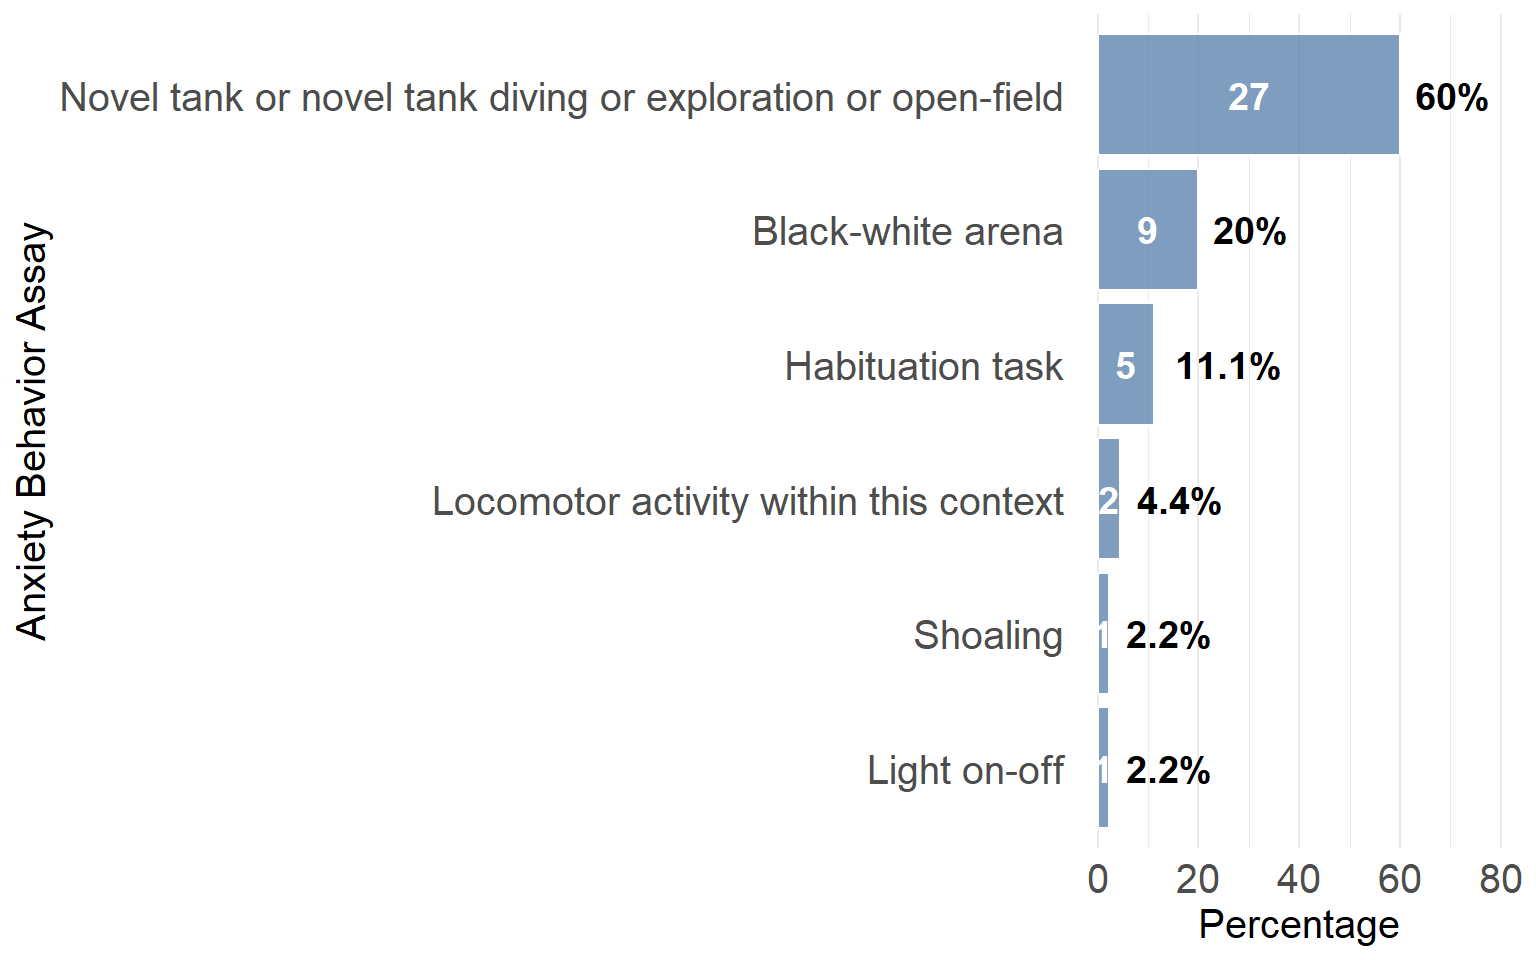
\includegraphics{zf_sm_code_files/figure-latex/unnamed-chunk-29-1.pdf}

\hypertarget{figs21---heat-map-to-show-which-life-stages-of-exposure-have-been-exposed-to-each-target-chemical-class}{%
\subsection{figs21 - heat map to show which life stages of exposure have
been exposed to each target chemical
class}\label{figs21---heat-map-to-show-which-life-stages-of-exposure-have-been-exposed-to-each-target-chemical-class}}

\begin{Shaded}
\begin{Highlighting}[]
\CommentTok{\# Separate rows by life\_stage\_exposure and pesticide\_target\_class columns}
\NormalTok{sd\_pd2 }\OtherTok{\textless{}{-}} \FunctionTok{separate\_rows}\NormalTok{(sd\_pd, life\_stage\_exposure, }\AttributeTok{sep =} \StringTok{","}\NormalTok{, }\AttributeTok{convert =} \ConstantTok{TRUE}\NormalTok{)}
\NormalTok{sd\_pd2 }\OtherTok{\textless{}{-}} \FunctionTok{separate\_rows}\NormalTok{(sd\_pd2, pesticide\_target\_class, }\AttributeTok{sep =} \StringTok{","}\NormalTok{, }\AttributeTok{convert =} \ConstantTok{TRUE}\NormalTok{)}

\CommentTok{\# Group by "life\_stage\_exposure" and "pesticide\_target\_class" and summarize count}
\NormalTok{sd\_pd\_summary2 }\OtherTok{\textless{}{-}}\NormalTok{ sd\_pd2 }\SpecialCharTok{\%\textgreater{}\%}
  \FunctionTok{mutate}\NormalTok{(}\AttributeTok{life\_stage\_exposure =} \FunctionTok{str\_trim}\NormalTok{(life\_stage\_exposure),}
         \AttributeTok{pesticide\_target\_class =} \FunctionTok{str\_trim}\NormalTok{(pesticide\_target\_class)) }\SpecialCharTok{\%\textgreater{}\%}
  \FunctionTok{group\_by}\NormalTok{(life\_stage\_exposure, pesticide\_target\_class) }\SpecialCharTok{\%\textgreater{}\%}
  \FunctionTok{summarise}\NormalTok{(}\AttributeTok{count =} \FunctionTok{n}\NormalTok{()) }\SpecialCharTok{\%\textgreater{}\%}
  \FunctionTok{ungroup}\NormalTok{()}
\end{Highlighting}
\end{Shaded}

\begin{verbatim}
## `summarise()` has grouped output by 'life_stage_exposure'. You can override
## using the `.groups` argument.
\end{verbatim}

\begin{Shaded}
\begin{Highlighting}[]
\CommentTok{\# Create a heatmap with pesticide target class on the x{-}axis and life stage exposure on the y{-}axis}
\NormalTok{figs21 }\OtherTok{\textless{}{-}} \FunctionTok{ggplot}\NormalTok{(sd\_pd\_summary2, }\FunctionTok{aes}\NormalTok{(}\AttributeTok{x =}\NormalTok{ pesticide\_target\_class, }\AttributeTok{y =}\NormalTok{ life\_stage\_exposure, }\AttributeTok{fill =}\NormalTok{ count)) }\SpecialCharTok{+}
  
  \CommentTok{\#Create and fill each tile}
  \FunctionTok{geom\_tile}\NormalTok{(}\AttributeTok{color =} \StringTok{"white"}\NormalTok{) }\SpecialCharTok{+}
  \FunctionTok{scale\_fill\_gradient}\NormalTok{(}\AttributeTok{low =} \StringTok{"\#F0F4F8"}\NormalTok{, }\AttributeTok{high =} \StringTok{"\#446487"}\NormalTok{) }\SpecialCharTok{+}
  
  \CommentTok{\# Add labels to the bars for absolute count }
  \FunctionTok{geom\_text}\NormalTok{(}\FunctionTok{aes}\NormalTok{(}\AttributeTok{label =} \FunctionTok{ifelse}\NormalTok{(count }\SpecialCharTok{\textgreater{}} \DecValTok{0}\NormalTok{, count, }\StringTok{""}\NormalTok{)), }\AttributeTok{color =} \StringTok{"black"}\NormalTok{, }\AttributeTok{size =} \DecValTok{4}\NormalTok{) }\SpecialCharTok{+}
  
  \CommentTok{\# Add axis and plot labels}
  \FunctionTok{labs}\NormalTok{(}\AttributeTok{x =} \StringTok{"Pesticide Target Class"}\NormalTok{, }\AttributeTok{y =} \StringTok{"Life Stage Exposure"}\NormalTok{, }\AttributeTok{fill =} \StringTok{"Count"}\NormalTok{) }\SpecialCharTok{+}
  
  \CommentTok{\# Customize the plot theme}
  \FunctionTok{theme\_minimal}\NormalTok{() }\SpecialCharTok{+}
  \FunctionTok{theme}\NormalTok{(}\AttributeTok{panel.grid.major.y =} \FunctionTok{element\_blank}\NormalTok{(),}
    \AttributeTok{axis.line.y =} \FunctionTok{element\_blank}\NormalTok{(),}
    \AttributeTok{axis.ticks.y =} \FunctionTok{element\_blank}\NormalTok{(),}
    \AttributeTok{axis.text.x =} \FunctionTok{element\_text}\NormalTok{(}\AttributeTok{size =} \DecValTok{15}\NormalTok{),}
    \AttributeTok{axis.text.y =} \FunctionTok{element\_text}\NormalTok{(}\AttributeTok{size =} \DecValTok{15}\NormalTok{, }\AttributeTok{hjust =} \DecValTok{1}\NormalTok{),}
    \AttributeTok{axis.title.x =} \FunctionTok{element\_text}\NormalTok{(}\AttributeTok{size =} \DecValTok{15}\NormalTok{),}
    \AttributeTok{axis.title.y =} \FunctionTok{element\_text}\NormalTok{(}\AttributeTok{size =} \DecValTok{15}\NormalTok{),}
    \AttributeTok{plot.title =} \FunctionTok{element\_blank}\NormalTok{())}
\NormalTok{figs21                                     }
\end{Highlighting}
\end{Shaded}

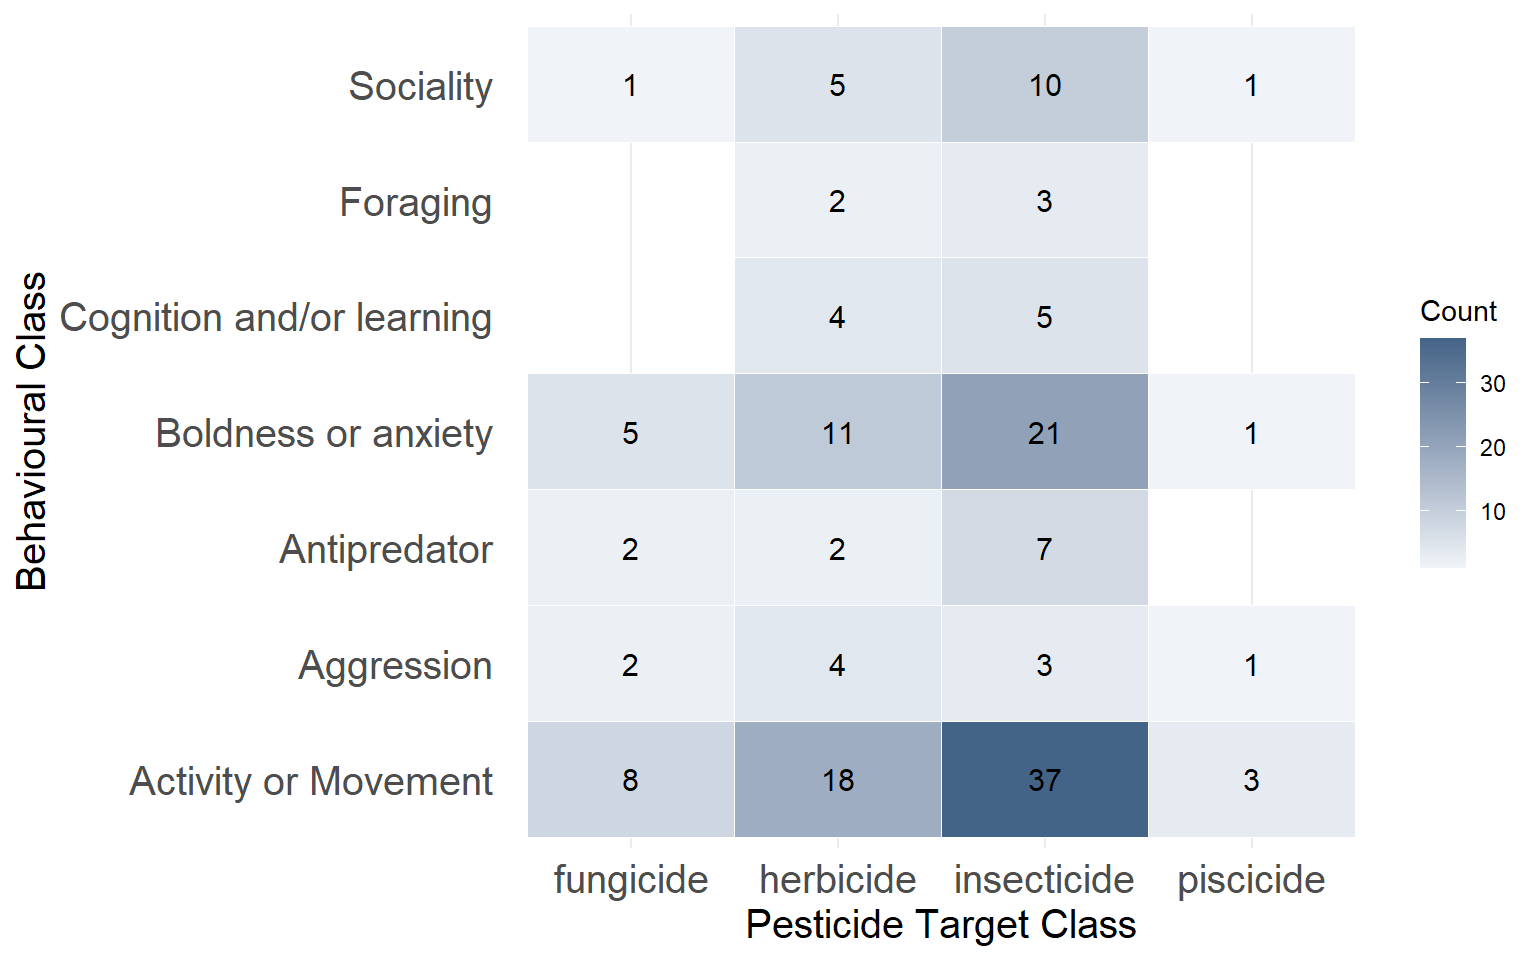
\includegraphics{zf_sm_code_files/figure-latex/unnamed-chunk-30-1.pdf}

\hypertarget{objective-4.-to-examine-how-are-authors-connected-between-countries-and-how-is-the-literature-connected-between-and-within-disciplines.}{%
\section{Objective 4. To examine how are authors connected between
countries and how is the literature connected between and within
disciplines.}\label{objective-4.-to-examine-how-are-authors-connected-between-countries-and-how-is-the-literature-connected-between-and-within-disciplines.}}

\hypertarget{figs24---general-bibliometric-summaries}{%
\subsection{figs24 - general bibliometric
summaries}\label{figs24---general-bibliometric-summaries}}

\begin{Shaded}
\begin{Highlighting}[]
\CommentTok{\# Perform bibliometric analysis on dataset "bib\_sco"}
\NormalTok{figs24 }\OtherTok{\textless{}{-}} \FunctionTok{biblioAnalysis}\NormalTok{(bib\_sco)}

\CommentTok{\# Display the plot of the analysis results}
\FunctionTok{plot}\NormalTok{(figs24)}
\end{Highlighting}
\end{Shaded}

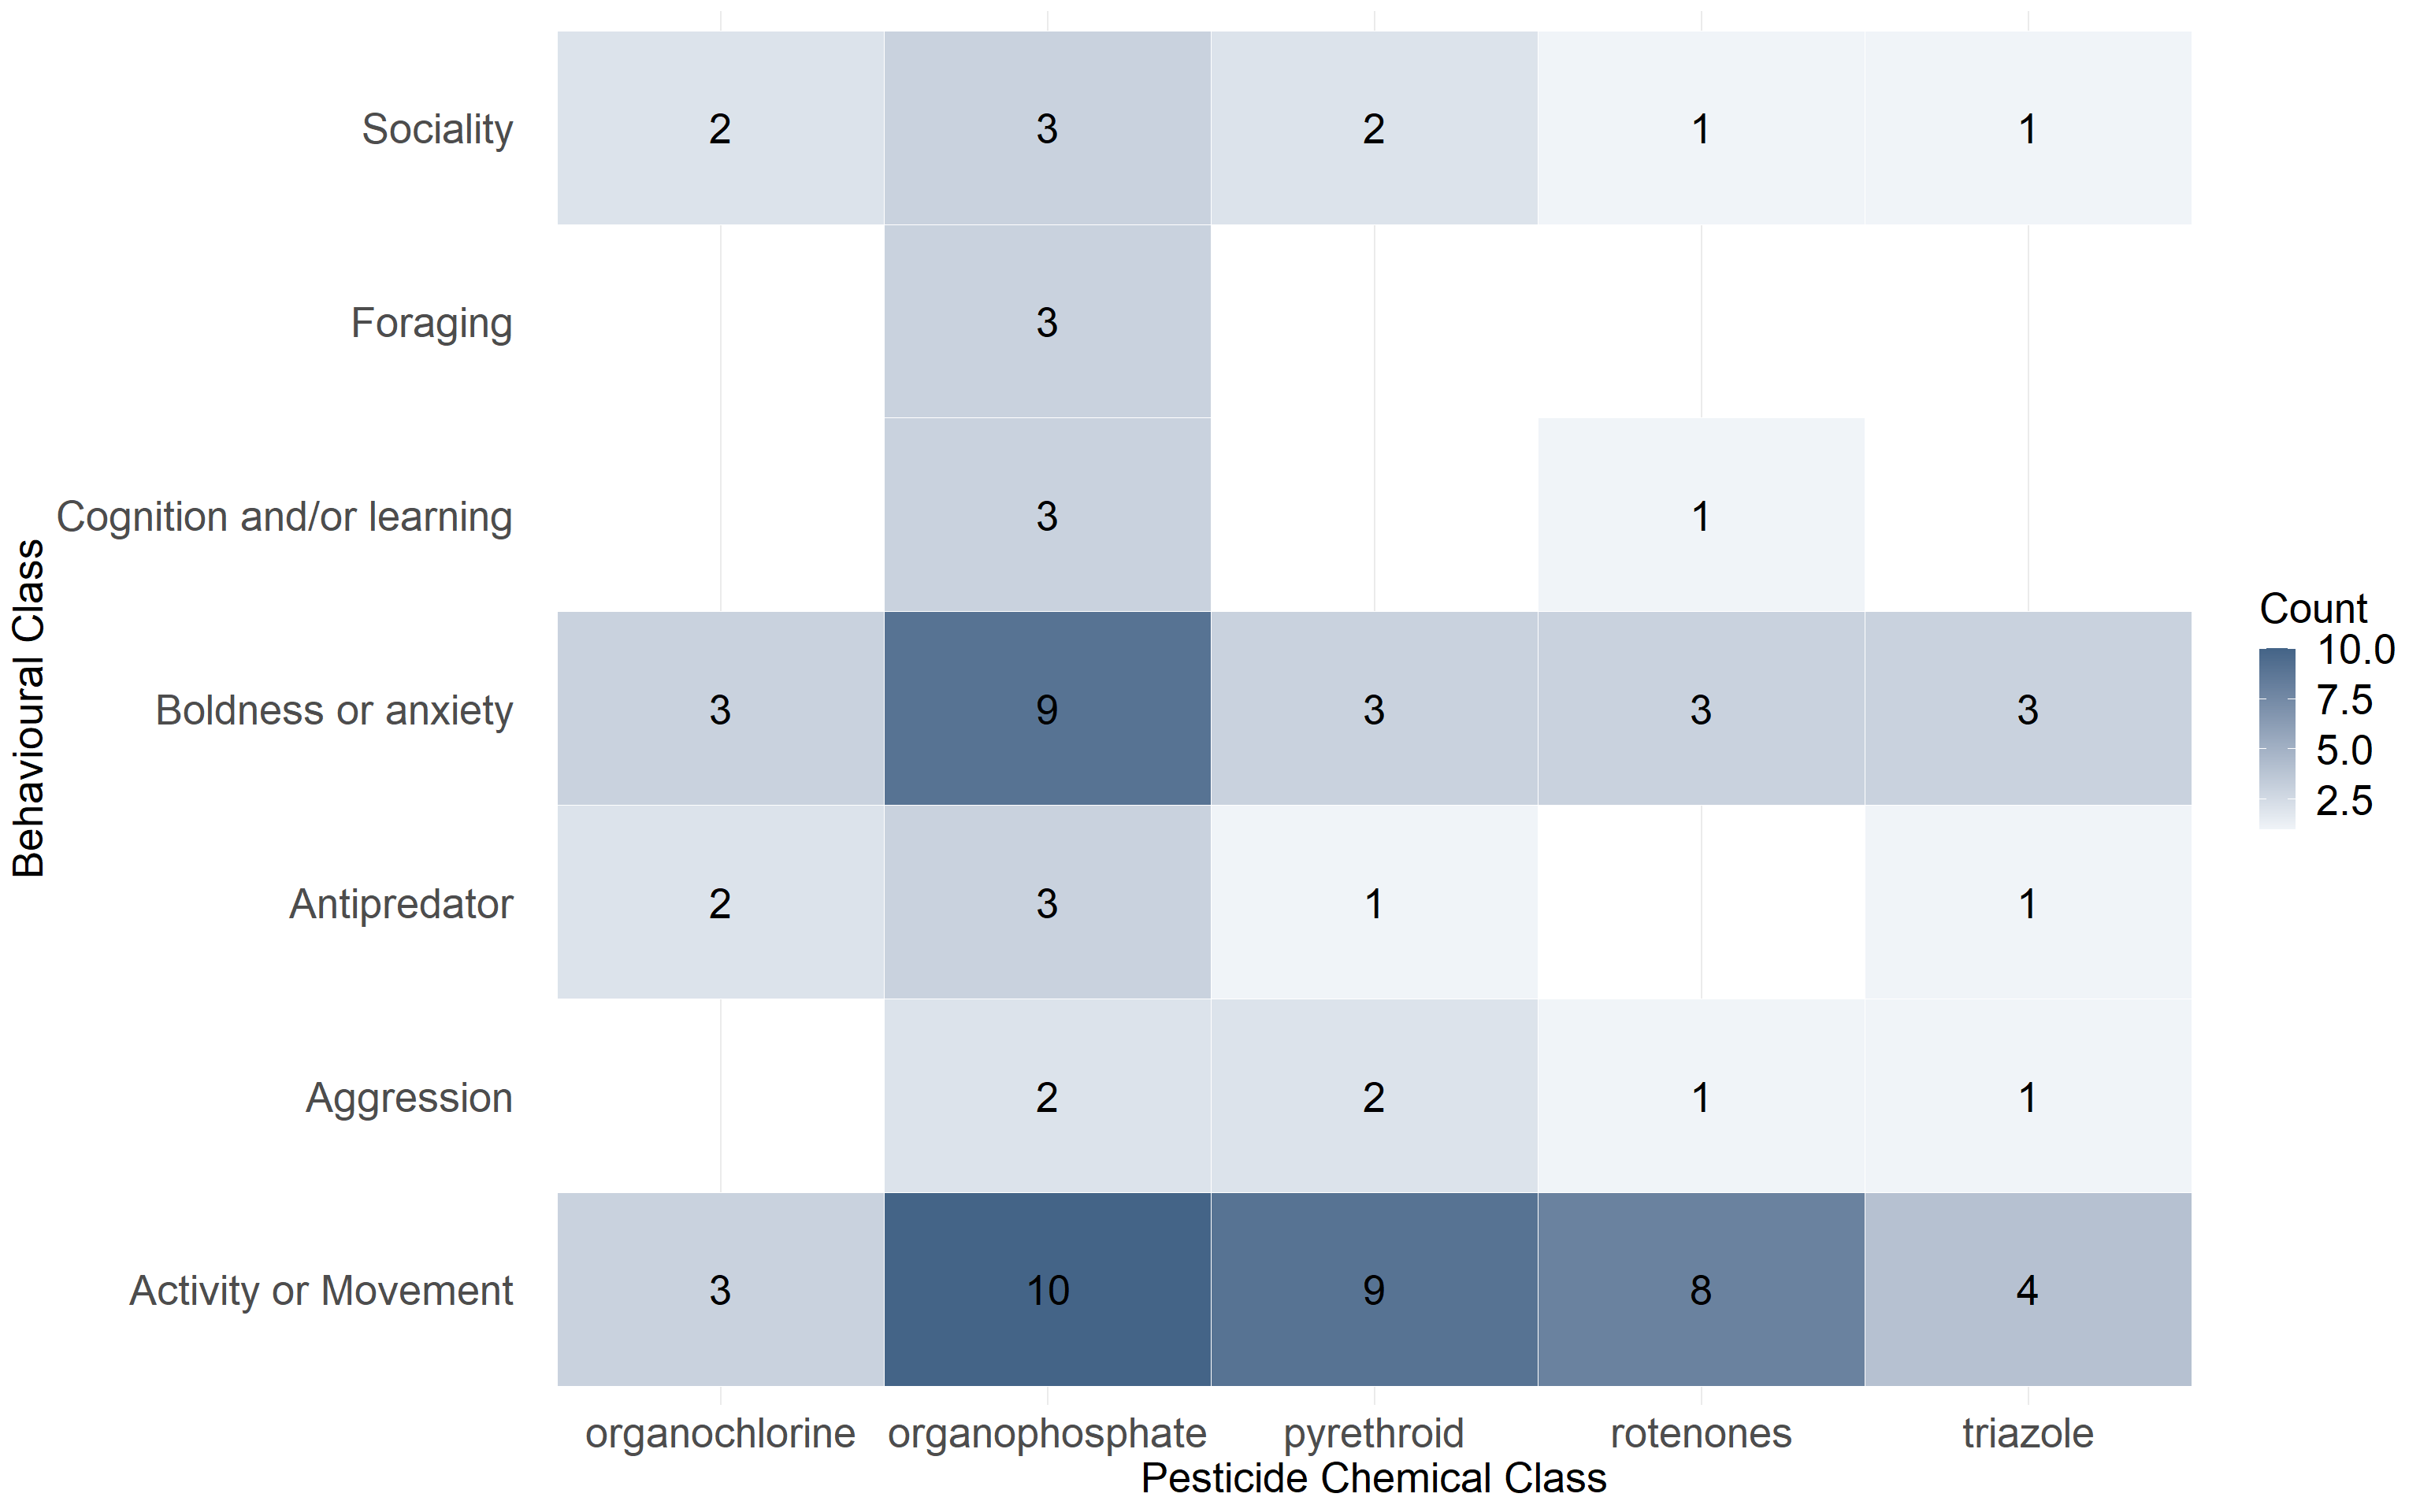
\includegraphics{zf_sm_code_files/figure-latex/unnamed-chunk-31-1.pdf}
\includegraphics{zf_sm_code_files/figure-latex/unnamed-chunk-31-2.pdf}
\includegraphics{zf_sm_code_files/figure-latex/unnamed-chunk-31-3.pdf}
\includegraphics{zf_sm_code_files/figure-latex/unnamed-chunk-31-4.pdf}
\includegraphics{zf_sm_code_files/figure-latex/unnamed-chunk-31-5.pdf}

\hypertarget{figs27---co-occurance-matrix}{%
\subsection{figs27 - co-occurance
matrix}\label{figs27---co-occurance-matrix}}

\begin{Shaded}
\begin{Highlighting}[]
\CommentTok{\# Generate a bibliometric network based on co{-}occurrences of keywords in the "bib\_sco" dataset}
\NormalTok{NetMatrix\_keywords }\OtherTok{\textless{}{-}} \FunctionTok{biblioNetwork}\NormalTok{(bib\_sco, }\AttributeTok{analysis =} \StringTok{"co{-}occurrences"}\NormalTok{, }\AttributeTok{network =} \StringTok{"keywords"}\NormalTok{, }\AttributeTok{sep =} \StringTok{";"}\NormalTok{)}

\CommentTok{\# Plot the network using the "networkPlot" function, with various formatting options}
\NormalTok{figs25 }\OtherTok{\textless{}{-}} \FunctionTok{networkPlot}\NormalTok{(NetMatrix\_keywords, }\AttributeTok{normalize=}\StringTok{"association"}\NormalTok{, }\AttributeTok{n =} \DecValTok{10}\NormalTok{, }
                     \AttributeTok{Title =} \StringTok{"Keyword Co{-}occurrences"}\NormalTok{, }\AttributeTok{type =} \StringTok{"fruchterman"}\NormalTok{, }
                     \AttributeTok{size.cex =} \ConstantTok{TRUE}\NormalTok{, }\AttributeTok{size =} \DecValTok{10}\NormalTok{, }\AttributeTok{remove.multiple =}\NormalTok{ F, }
                     \AttributeTok{edgesize =} \DecValTok{4}\NormalTok{, }\AttributeTok{labelsize =} \DecValTok{3}\NormalTok{, }\AttributeTok{label.cex =} \ConstantTok{TRUE}\NormalTok{, }
                     \AttributeTok{edges.min =} \DecValTok{2}\NormalTok{, }\AttributeTok{label.n =} \DecValTok{10}\NormalTok{, }\AttributeTok{alpha =} \FloatTok{0.3}\NormalTok{)}
\end{Highlighting}
\end{Shaded}

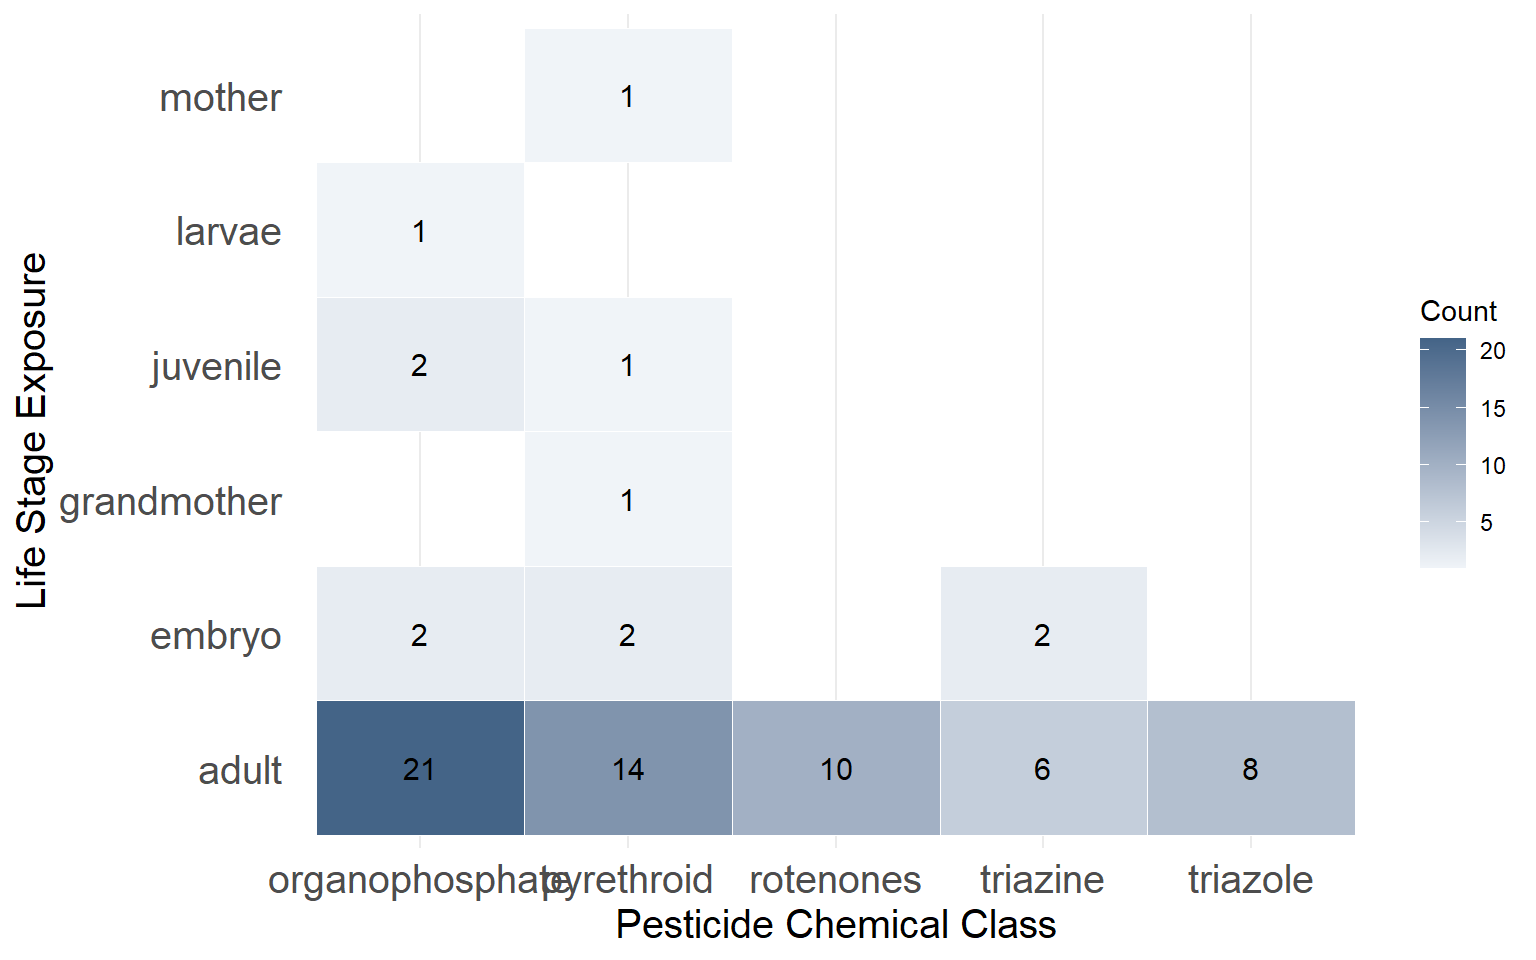
\includegraphics{zf_sm_code_files/figure-latex/unnamed-chunk-32-1.pdf}

\hypertarget{fig-s26---thematic-map-based-on-keywords}{%
\subsection{fig s26 - thematic map based on
keywords}\label{fig-s26---thematic-map-based-on-keywords}}

\begin{Shaded}
\begin{Highlighting}[]
\CommentTok{\# Set plot parameters to display a single plot with narrow margins}
\FunctionTok{par}\NormalTok{(}\AttributeTok{mfrow=}\FunctionTok{c}\NormalTok{(}\DecValTok{1}\NormalTok{,}\DecValTok{1}\NormalTok{), }\AttributeTok{mar=}\FunctionTok{c}\NormalTok{(}\DecValTok{0}\NormalTok{,}\DecValTok{2}\NormalTok{,}\DecValTok{0}\NormalTok{,}\DecValTok{2}\NormalTok{))}

\CommentTok{\# Generate a thematic map of the "bib\_sco" dataset, using the "ID" field as the basis for the map}
\NormalTok{figs26 }\OtherTok{\textless{}{-}} \FunctionTok{thematicMap}\NormalTok{(bib\_sco, }\AttributeTok{field =} \StringTok{"ID"}\NormalTok{, }\AttributeTok{n =} \DecValTok{1000}\NormalTok{, }\AttributeTok{minfreq =} \DecValTok{5}\NormalTok{, }\AttributeTok{stemming =} \ConstantTok{FALSE}\NormalTok{, }\AttributeTok{size =} \FloatTok{0.5}\NormalTok{, }\AttributeTok{n.labels =} \DecValTok{1}\NormalTok{, }\AttributeTok{repel =} \ConstantTok{TRUE}\NormalTok{)}

\CommentTok{\# Display the resulting map using the "plot" function}
\FunctionTok{plot}\NormalTok{(figs26}\SpecialCharTok{$}\NormalTok{map)}
\end{Highlighting}
\end{Shaded}

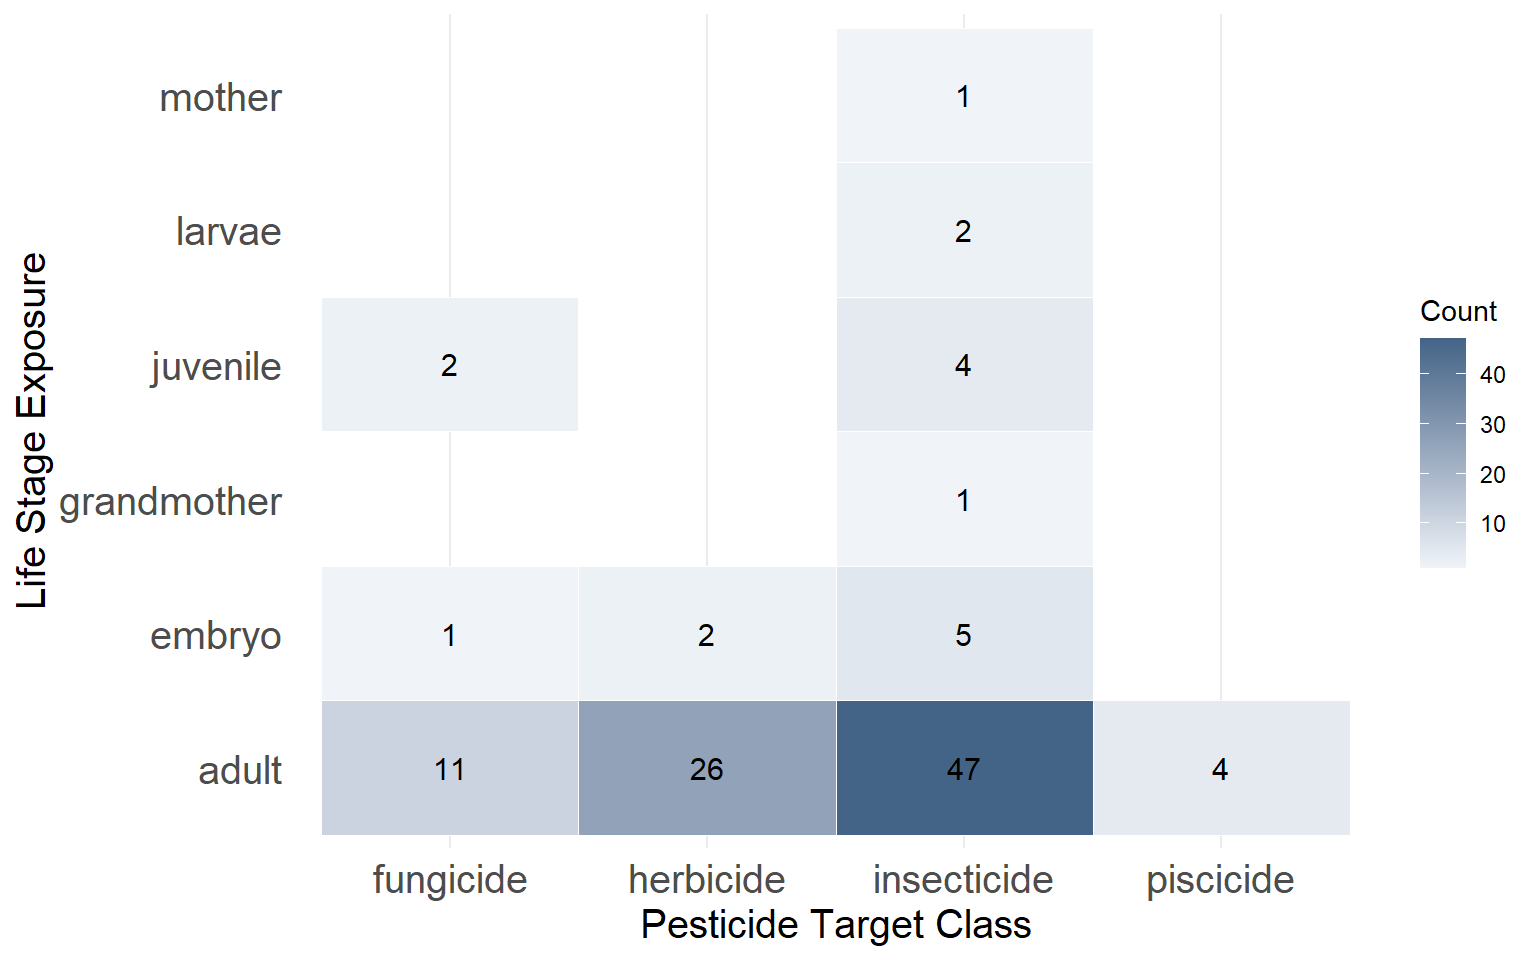
\includegraphics{zf_sm_code_files/figure-latex/unnamed-chunk-33-1.pdf}

\hypertarget{fig6---country-publications-map}{%
\subsection{fig6 - country publications
map}\label{fig6---country-publications-map}}

\begin{Shaded}
\begin{Highlighting}[]
\CommentTok{\# Extract country information from the "AU1\_CO" and "AU\_CO" fields of the "bib\_sco" dataset}
\NormalTok{bibmap }\OtherTok{\textless{}{-}} \FunctionTok{metaTagExtraction}\NormalTok{(bib\_sco, }\AttributeTok{Field =} \StringTok{"AU1\_CO"}\NormalTok{, }\AttributeTok{sep =} \StringTok{";"}\NormalTok{) }
\NormalTok{bibmap }\OtherTok{\textless{}{-}} \FunctionTok{metaTagExtraction}\NormalTok{(bibmap, }\AttributeTok{Field =} \StringTok{"AU\_CO"}\NormalTok{, }\AttributeTok{sep =} \StringTok{";"}\NormalTok{) }

\CommentTok{\# Create a data frame with counts of articles from each country}
\NormalTok{bibmap }\SpecialCharTok{\%\textgreater{}\%} 
  \FunctionTok{group\_by}\NormalTok{(AU1\_CO) }\SpecialCharTok{\%\textgreater{}\%} 
  \FunctionTok{count}\NormalTok{() }\SpecialCharTok{\%\textgreater{}\%} 
  \FunctionTok{filter}\NormalTok{(}\SpecialCharTok{!}\FunctionTok{is.na}\NormalTok{(AU1\_CO)) }\OtherTok{{-}\textgreater{}}\NormalTok{ firstcountrycounts}

\CommentTok{\# Load world map data and remove countries with longitude \textgreater{}180 to make an equal projection{-}like map}
\NormalTok{world\_map }\OtherTok{\textless{}{-}} \FunctionTok{map\_data}\NormalTok{(}\StringTok{"world"}\NormalTok{) }\SpecialCharTok{\%\textgreater{}\%} 
  \FunctionTok{filter}\NormalTok{(}\SpecialCharTok{!}\NormalTok{ long }\SpecialCharTok{\textgreater{}} \DecValTok{180}\NormalTok{)}

\CommentTok{\# Format country names to match regions on the world map}
\NormalTok{firstcountrycounts}\SpecialCharTok{$}\NormalTok{region }\OtherTok{\textless{}{-}} \FunctionTok{str\_to\_title}\NormalTok{(firstcountrycounts}\SpecialCharTok{$}\NormalTok{AU1\_CO)}
\NormalTok{firstcountrycounts}\SpecialCharTok{$}\NormalTok{region[firstcountrycounts}\SpecialCharTok{$}\NormalTok{region }\SpecialCharTok{==} \StringTok{"Usa"}\NormalTok{] }\OtherTok{\textless{}{-}} \StringTok{"USA"} 
\NormalTok{firstcountrycounts}\SpecialCharTok{$}\NormalTok{region[firstcountrycounts}\SpecialCharTok{$}\NormalTok{region }\SpecialCharTok{==} \StringTok{"Korea"}\NormalTok{] }\OtherTok{\textless{}{-}} \StringTok{"South Korea"}

\CommentTok{\# Join count data with map data and set missing counts to zero}
\NormalTok{emptymap }\OtherTok{\textless{}{-}} \FunctionTok{tibble}\NormalTok{(}\AttributeTok{region =} \FunctionTok{unique}\NormalTok{(world\_map}\SpecialCharTok{$}\NormalTok{region), }\AttributeTok{n =} \FunctionTok{rep}\NormalTok{(}\DecValTok{0}\NormalTok{,}\FunctionTok{length}\NormalTok{(}\FunctionTok{unique}\NormalTok{(world\_map}\SpecialCharTok{$}\NormalTok{region))))}
\NormalTok{fullmap }\OtherTok{\textless{}{-}} \FunctionTok{left\_join}\NormalTok{(emptymap, firstcountrycounts, }\AttributeTok{by =} \StringTok{"region"}\NormalTok{)}
\NormalTok{fullmap}\SpecialCharTok{$}\NormalTok{n }\OtherTok{\textless{}{-}}\NormalTok{ fullmap}\SpecialCharTok{$}\NormalTok{n.x }\SpecialCharTok{+}\NormalTok{ fullmap}\SpecialCharTok{$}\NormalTok{n.y}
\NormalTok{fullmap}\SpecialCharTok{$}\NormalTok{n[}\FunctionTok{is.na}\NormalTok{(fullmap}\SpecialCharTok{$}\NormalTok{n)] }\OtherTok{\textless{}{-}} \DecValTok{0}

\CommentTok{\# Create a plot of the world map with regions colored based on article counts}
\NormalTok{figs27 }\OtherTok{\textless{}{-}}\NormalTok{ fullmap }\SpecialCharTok{\%\textgreater{}\%} 
  \FunctionTok{ggplot}\NormalTok{(}\FunctionTok{aes}\NormalTok{(}\AttributeTok{fill =}\NormalTok{ n, }\AttributeTok{map\_id =}\NormalTok{ region)) }\SpecialCharTok{+}
  \FunctionTok{geom\_map}\NormalTok{(}\AttributeTok{map =}\NormalTok{ world\_map) }\SpecialCharTok{+}
  \FunctionTok{expand\_limits}\NormalTok{(}\AttributeTok{x =}\NormalTok{ world\_map}\SpecialCharTok{$}\NormalTok{long, }\AttributeTok{y =}\NormalTok{ world\_map}\SpecialCharTok{$}\NormalTok{lat) }\SpecialCharTok{+}
  \FunctionTok{coord\_map}\NormalTok{(}\StringTok{"moll"}\NormalTok{) }\SpecialCharTok{+} \CommentTok{\# Mollweide projection}
  \FunctionTok{theme\_map}\NormalTok{(}\AttributeTok{line\_size =} \FloatTok{0.5}\NormalTok{) }\SpecialCharTok{+} 
  \FunctionTok{scale\_fill\_gradient}\NormalTok{(}\AttributeTok{low =} \StringTok{"\#ECF207"}\NormalTok{, }\AttributeTok{high =} \StringTok{"\#C307F2"}\NormalTok{, }\CommentTok{\# set color gradient}
                    \AttributeTok{name =} \StringTok{"Score"}\NormalTok{, }\AttributeTok{na.value =} \StringTok{"gray"}\NormalTok{,}
                    \AttributeTok{limits =} \FunctionTok{c}\NormalTok{(}\FloatTok{0.1}\NormalTok{, }\DecValTok{24}\NormalTok{),}
                    \AttributeTok{guide =} \FunctionTok{guide\_colorbar}\NormalTok{(}\AttributeTok{direction =} \StringTok{"vertical."}\NormalTok{,}
                                           \AttributeTok{barwidth =} \FunctionTok{unit}\NormalTok{(}\DecValTok{15}\NormalTok{, }\AttributeTok{units =} \StringTok{"mm"}\NormalTok{), }
                                           \AttributeTok{barheight =} \FunctionTok{unit}\NormalTok{(}\DecValTok{50}\NormalTok{, }\AttributeTok{units =} \StringTok{"mm"}\NormalTok{))) }\SpecialCharTok{+}
  \FunctionTok{guides}\NormalTok{(}\AttributeTok{fill =} \FunctionTok{guide\_colourbar}\NormalTok{()) }\SpecialCharTok{+}
  \FunctionTok{theme}\NormalTok{(}\AttributeTok{panel.background =} \FunctionTok{element\_rect}\NormalTok{(}\AttributeTok{fill =} \StringTok{"transparent"}\NormalTok{, }\AttributeTok{colour =} \ConstantTok{NA}\NormalTok{),}
        \AttributeTok{plot.background =} \FunctionTok{element\_rect}\NormalTok{(}\AttributeTok{fill =} \StringTok{"transparent"}\NormalTok{, }\AttributeTok{colour =} \ConstantTok{NA}\NormalTok{))}
  
\NormalTok{figs27}
\end{Highlighting}
\end{Shaded}

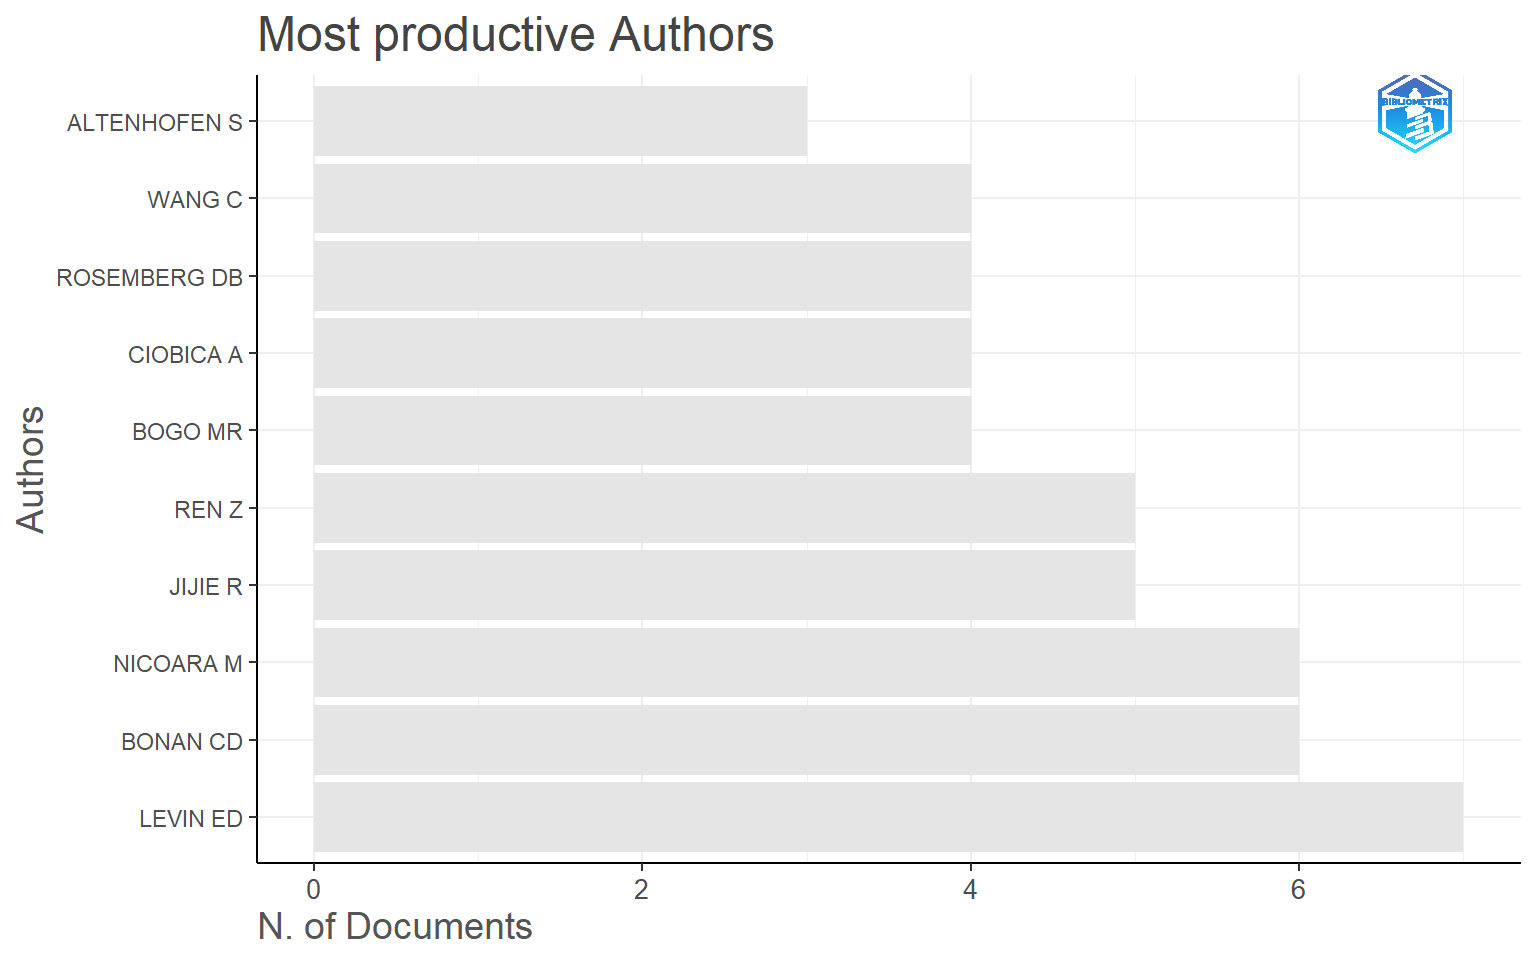
\includegraphics{zf_sm_code_files/figure-latex/unnamed-chunk-34-1.pdf}

\begin{Shaded}
\begin{Highlighting}[]
\CommentTok{\# ggsave(here("figures", "world\_map.png"), width = 16, height = 10, units = "cm", scale = 2, dpi = 300)}
\end{Highlighting}
\end{Shaded}

\hypertarget{figs28---country-collaboration-network-circle-plot}{%
\subsection{figs28 - country collaboration network circle
plot}\label{figs28---country-collaboration-network-circle-plot}}

\begin{Shaded}
\begin{Highlighting}[]
\CommentTok{\# Extract countries from the affiliations}
\NormalTok{bib\_sco2 }\OtherTok{\textless{}{-}} \FunctionTok{metaTagExtraction}\NormalTok{(bib\_sco, }\AttributeTok{Field =} \StringTok{"AU\_CO"}\NormalTok{, }\AttributeTok{sep =} \StringTok{";"}\NormalTok{)}

\CommentTok{\# Create a network matrix of collaborations between countries}
\NormalTok{NetMatrix\_country }\OtherTok{\textless{}{-}} \FunctionTok{biblioNetwork}\NormalTok{(bib\_sco2, }\AttributeTok{analysis =} \StringTok{"collaboration"}\NormalTok{, }\AttributeTok{network =} \StringTok{"countries"}\NormalTok{, }\AttributeTok{sep =} \StringTok{";"}\NormalTok{)}

\CommentTok{\# Convert the network matrix to a standard matrix}
\NormalTok{NetMatrix\_country }\OtherTok{\textless{}{-}} \FunctionTok{as.matrix}\NormalTok{(NetMatrix\_country)}

\CommentTok{\# Remove the lower triangle (as this is duplication of info)}
\NormalTok{NetMatrix\_country[}\FunctionTok{lower.tri}\NormalTok{(NetMatrix\_country)] }\OtherTok{\textless{}{-}} \DecValTok{0} 

\CommentTok{\# Change column and row names to title case}
\FunctionTok{colnames}\NormalTok{(NetMatrix\_country) }\OtherTok{\textless{}{-}} \FunctionTok{str\_to\_title}\NormalTok{(}\FunctionTok{colnames}\NormalTok{(NetMatrix\_country))}
\FunctionTok{rownames}\NormalTok{(NetMatrix\_country) }\OtherTok{\textless{}{-}} \FunctionTok{str\_to\_title}\NormalTok{(}\FunctionTok{rownames}\NormalTok{(NetMatrix\_country))}

\CommentTok{\# Change "Usa" to "USA"}
\FunctionTok{colnames}\NormalTok{(NetMatrix\_country)[}\FunctionTok{colnames}\NormalTok{(NetMatrix\_country) }\SpecialCharTok{==} \StringTok{"Usa"}\NormalTok{] }\OtherTok{\textless{}{-}} \StringTok{"USA"}
\FunctionTok{rownames}\NormalTok{(NetMatrix\_country)[}\FunctionTok{rownames}\NormalTok{(NetMatrix\_country) }\SpecialCharTok{==} \StringTok{"Usa"}\NormalTok{] }\OtherTok{\textless{}{-}} \StringTok{"USA"}

\CommentTok{\# Change "United Kingdom" to "UK" for easier plotting}
\FunctionTok{colnames}\NormalTok{(NetMatrix\_country)[}\FunctionTok{colnames}\NormalTok{(NetMatrix\_country) }\SpecialCharTok{==} \StringTok{"United Kingdom"}\NormalTok{] }\OtherTok{\textless{}{-}} \StringTok{"UK"}
\FunctionTok{rownames}\NormalTok{(NetMatrix\_country)[}\FunctionTok{rownames}\NormalTok{(NetMatrix\_country) }\SpecialCharTok{==} \StringTok{"United Kingdom"}\NormalTok{] }\OtherTok{\textless{}{-}} \StringTok{"UK"}

\NormalTok{my.cols2 }\OtherTok{\textless{}{-}} \FunctionTok{c}\NormalTok{(}
  \AttributeTok{USA =} \StringTok{"\#e41a1c"}\NormalTok{,}
  \AttributeTok{Canada =} \StringTok{"\#377eb8"}\NormalTok{,}
  \AttributeTok{Mexico =} \StringTok{"\#4daf4a"}\NormalTok{,}
  \AttributeTok{Brazil =} \StringTok{"\#984ea3"}\NormalTok{,}
  \AttributeTok{Ecuador =} \StringTok{"\#ff7f00"}\NormalTok{,}
  \AttributeTok{Chile =} \StringTok{"\#ffff33"}\NormalTok{,}
  \AttributeTok{Philippines =} \StringTok{"\#a65628"}\NormalTok{,}
  \AttributeTok{China =} \StringTok{"\#f781bf"}\NormalTok{,}
  \AttributeTok{Korea =} \StringTok{"\#e41a1c"}\NormalTok{,}
  \AttributeTok{India =} \StringTok{"\#984ea3"}\NormalTok{,}
  \AttributeTok{Turkey =} \StringTok{"\#ff7f00"}\NormalTok{,}
  \AttributeTok{Romania =} \StringTok{"\#4daf4a"}\NormalTok{,}
  \AttributeTok{Switzerland =} \StringTok{"\#377eb8"}\NormalTok{,}
  \AttributeTok{Norway =} \StringTok{"\#1b9e77"}\NormalTok{,}
  \AttributeTok{Netherlands =} \StringTok{"\#d95f02"}\NormalTok{,}
  \AttributeTok{Germany =} \StringTok{"\#7570b3"}\NormalTok{,}
  \AttributeTok{France =} \StringTok{"\#e7298a"}\NormalTok{,}
  \AttributeTok{Italy =} \StringTok{"\#66a61e"}\NormalTok{,}
  \AttributeTok{Portugal =} \StringTok{"\#e6ab02"}\NormalTok{,}
  \AttributeTok{Spain =} \StringTok{"\#a6761d"}\NormalTok{,}
  \AttributeTok{Sweden =} \StringTok{"\#666666"}
\NormalTok{)}

 

\CommentTok{\# Create a chord diagram of the network matrix}
\NormalTok{figs28 }\OtherTok{\textless{}{-}} \FunctionTok{chordDiagram}\NormalTok{(NetMatrix\_country, }\AttributeTok{annotationTrack =} \StringTok{"grid"}\NormalTok{, }\AttributeTok{preAllocateTracks =} \DecValTok{1}\NormalTok{, }\AttributeTok{grid.col =}\NormalTok{ my.cols2)}

\CommentTok{\# Add a track to label each sector with its name}
\FunctionTok{circos.trackPlotRegion}\NormalTok{(}\AttributeTok{track.index =} \DecValTok{1}\NormalTok{, }\AttributeTok{panel.fun =} \ControlFlowTok{function}\NormalTok{(x, y) \{}
\NormalTok{  xlim }\OtherTok{=} \FunctionTok{get.cell.meta.data}\NormalTok{(}\StringTok{"xlim"}\NormalTok{)}
\NormalTok{  ylim }\OtherTok{=} \FunctionTok{get.cell.meta.data}\NormalTok{(}\StringTok{"ylim"}\NormalTok{)}
\NormalTok{  sector.name }\OtherTok{=} \FunctionTok{get.cell.meta.data}\NormalTok{(}\StringTok{"sector.index"}\NormalTok{)}
  \FunctionTok{circos.text}\NormalTok{(}\FunctionTok{mean}\NormalTok{(xlim), ylim[}\DecValTok{1}\NormalTok{] }\SpecialCharTok{+}\NormalTok{ .}\DecValTok{1}\NormalTok{, sector.name, }\AttributeTok{facing =} \StringTok{"clockwise"}\NormalTok{, }\AttributeTok{niceFacing =} \ConstantTok{TRUE}\NormalTok{, }\AttributeTok{adj =} \FunctionTok{c}\NormalTok{(}\DecValTok{0}\NormalTok{, }\FloatTok{0.5}\NormalTok{))}
  \FunctionTok{circos.axis}\NormalTok{(}\AttributeTok{h =} \StringTok{"top"}\NormalTok{, }\AttributeTok{labels.cex =} \FloatTok{0.5}\NormalTok{, }\AttributeTok{major.tick.length =} \FloatTok{0.2}\NormalTok{, }\AttributeTok{sector.index =}\NormalTok{ sector.name, }\AttributeTok{track.index =} \DecValTok{2}\NormalTok{)}
\NormalTok{\}, }\AttributeTok{bg.border =} \ConstantTok{NA}\NormalTok{)}
\end{Highlighting}
\end{Shaded}

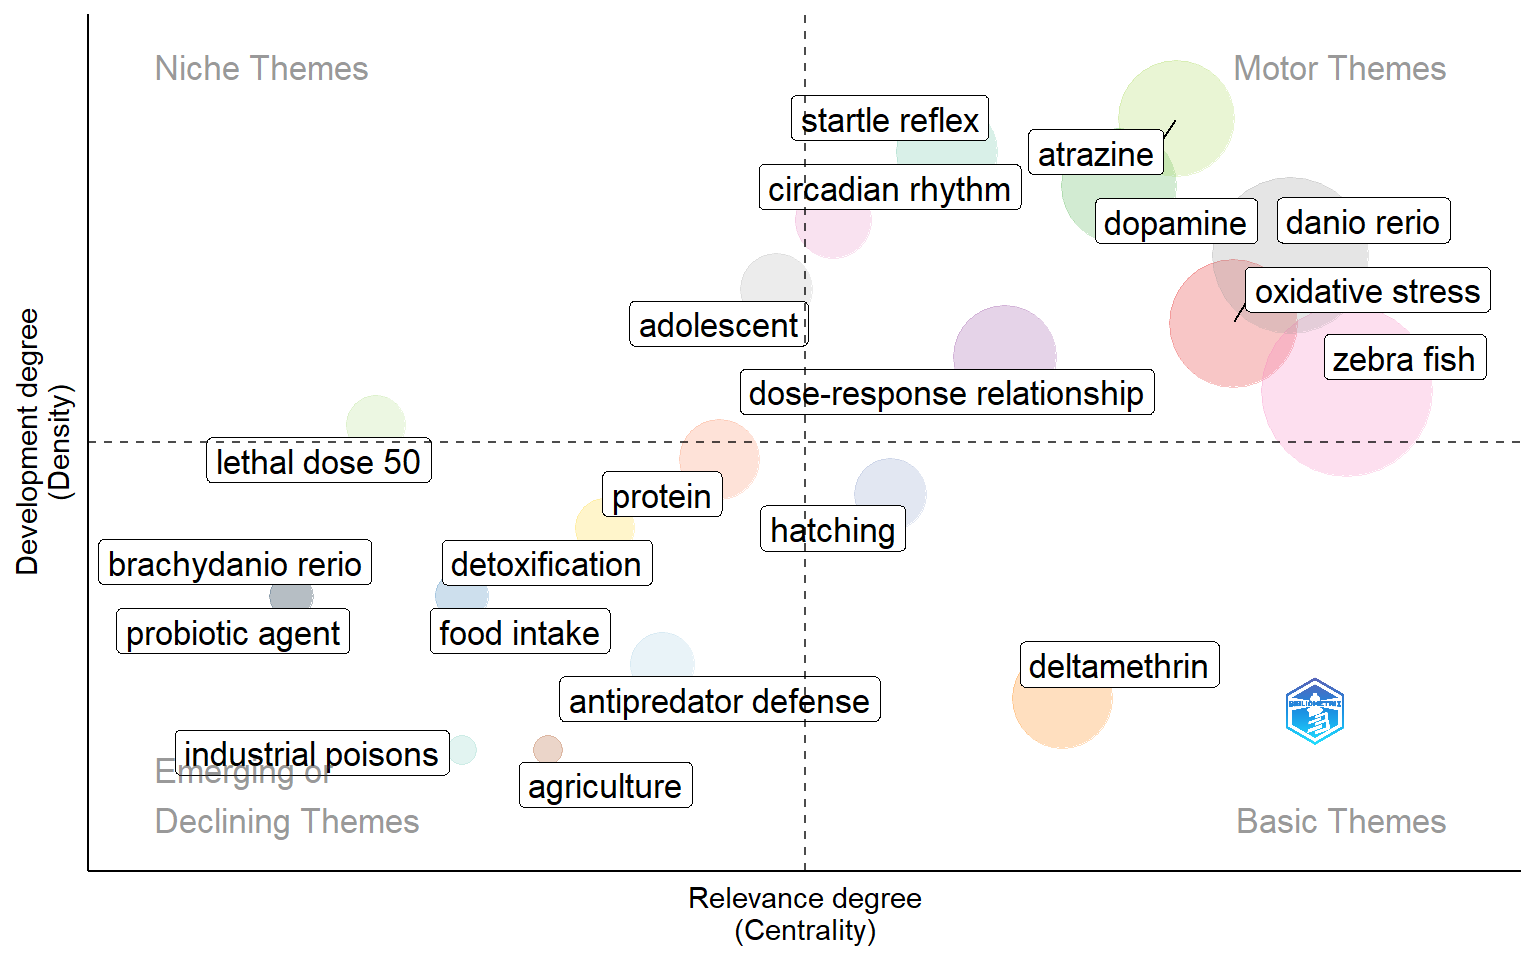
\includegraphics{zf_sm_code_files/figure-latex/unnamed-chunk-35-1.pdf}

\hypertarget{fig6a-collaboration-matrix-with-self-citation-removed}{%
\subsection{fig6a collaboration matrix with self citation
removed}\label{fig6a-collaboration-matrix-with-self-citation-removed}}

\begin{Shaded}
\begin{Highlighting}[]
\CommentTok{\# Making diagnol zero to remove self citations }
\FunctionTok{diag}\NormalTok{(NetMatrix\_country) }\OtherTok{\textless{}{-}} \DecValTok{0}

\CommentTok{\# Create a chord diagram of the network matrix}
\NormalTok{fig6a }\OtherTok{\textless{}{-}} \FunctionTok{chordDiagram}\NormalTok{(NetMatrix\_country, }\AttributeTok{annotationTrack =} \StringTok{"grid"}\NormalTok{, }\AttributeTok{preAllocateTracks =} \DecValTok{1}\NormalTok{, }\AttributeTok{grid.col =}\NormalTok{ my.cols2)}

\CommentTok{\# Add a track to label each sector with its name}
\FunctionTok{circos.trackPlotRegion}\NormalTok{(}\AttributeTok{track.index =} \DecValTok{1}\NormalTok{, }\AttributeTok{panel.fun =} \ControlFlowTok{function}\NormalTok{(x, y) \{}
\NormalTok{  xlim }\OtherTok{=} \FunctionTok{get.cell.meta.data}\NormalTok{(}\StringTok{"xlim"}\NormalTok{)}
\NormalTok{  ylim }\OtherTok{=} \FunctionTok{get.cell.meta.data}\NormalTok{(}\StringTok{"ylim"}\NormalTok{)}
\NormalTok{  sector.name }\OtherTok{=} \FunctionTok{get.cell.meta.data}\NormalTok{(}\StringTok{"sector.index"}\NormalTok{)}
  \FunctionTok{circos.text}\NormalTok{(}\FunctionTok{mean}\NormalTok{(xlim), ylim[}\DecValTok{1}\NormalTok{] }\SpecialCharTok{+}\NormalTok{ .}\DecValTok{1}\NormalTok{, sector.name, }\AttributeTok{facing =} \StringTok{"clockwise"}\NormalTok{, }\AttributeTok{niceFacing =} \ConstantTok{TRUE}\NormalTok{, }\AttributeTok{adj =} \FunctionTok{c}\NormalTok{(}\DecValTok{0}\NormalTok{, }\FloatTok{0.5}\NormalTok{))}
  \FunctionTok{circos.axis}\NormalTok{(}\AttributeTok{h =} \StringTok{"top"}\NormalTok{, }\AttributeTok{labels.cex =} \FloatTok{0.5}\NormalTok{, }\AttributeTok{major.tick.length =} \FloatTok{0.2}\NormalTok{, }\AttributeTok{sector.index =}\NormalTok{ sector.name, }\AttributeTok{track.index =} \DecValTok{2}\NormalTok{)}
\NormalTok{\}, }\AttributeTok{bg.border =} \ConstantTok{NA}\NormalTok{)}
\end{Highlighting}
\end{Shaded}

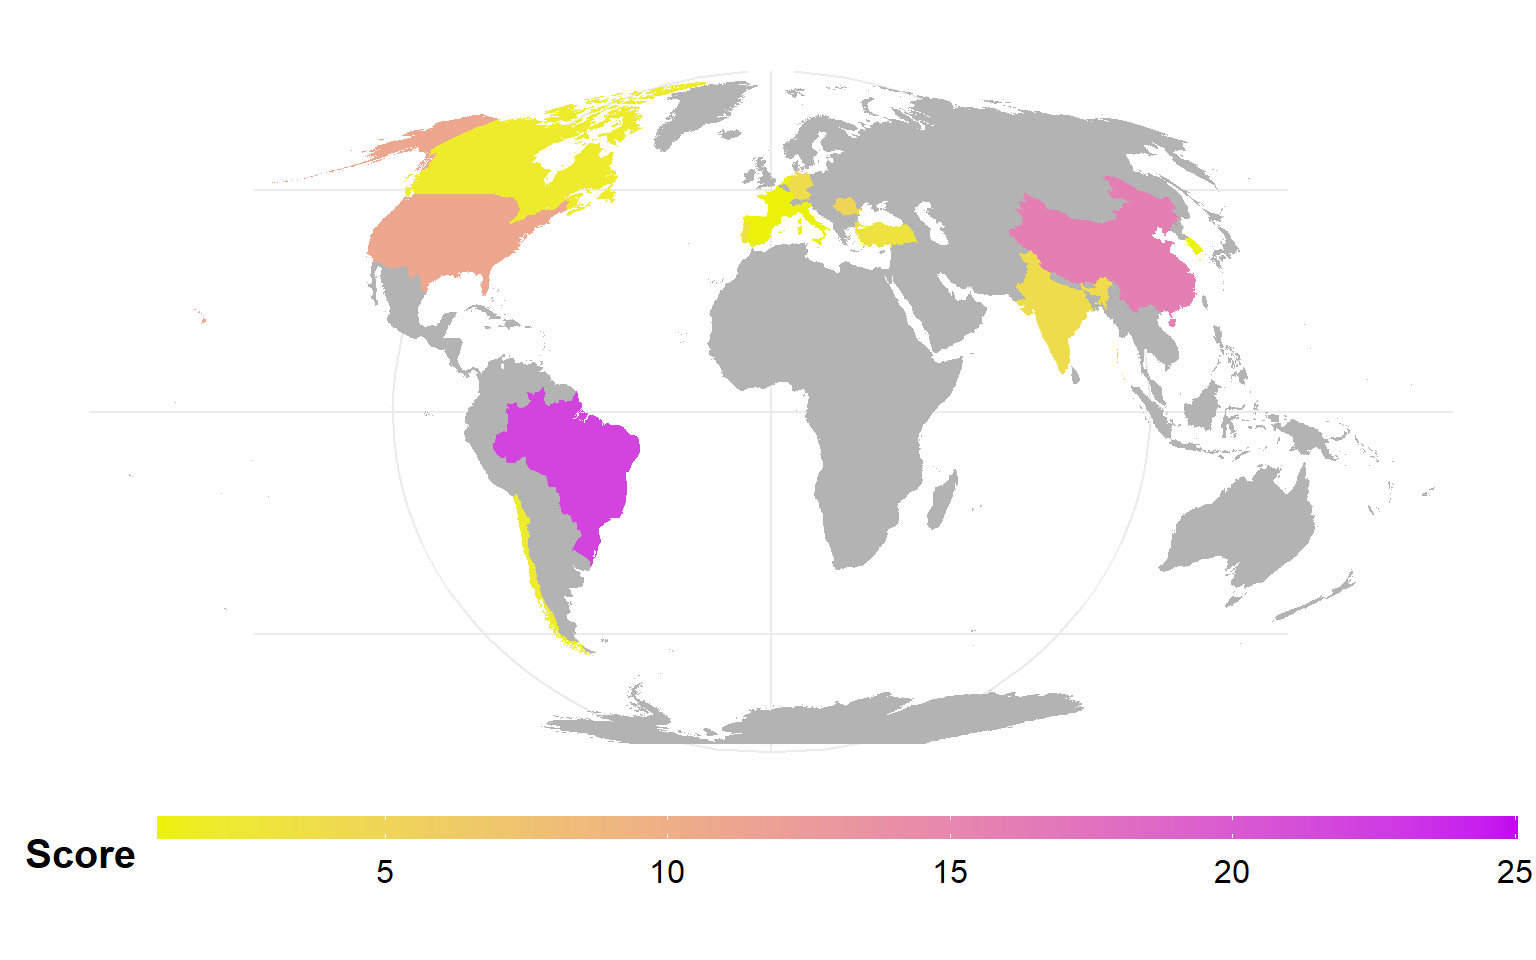
\includegraphics{zf_sm_code_files/figure-latex/unnamed-chunk-36-1.pdf}

\hypertarget{fig6b-continent-collaboration}{%
\subsection{fig6b continent
collaboration}\label{fig6b-continent-collaboration}}

\begin{Shaded}
\begin{Highlighting}[]
\NormalTok{NetMatrix\_continent }\OtherTok{\textless{}{-}}\NormalTok{ NetMatrix\_country}
\CommentTok{\# Change "Usa" to "North America"}
\FunctionTok{colnames}\NormalTok{(NetMatrix\_continent)[}\FunctionTok{colnames}\NormalTok{(NetMatrix\_continent) }\SpecialCharTok{==} \StringTok{"USA"}\NormalTok{] }\OtherTok{\textless{}{-}} \StringTok{"North America"}
\FunctionTok{rownames}\NormalTok{(NetMatrix\_continent)[}\FunctionTok{rownames}\NormalTok{(NetMatrix\_continent) }\SpecialCharTok{==} \StringTok{"USA"}\NormalTok{] }\OtherTok{\textless{}{-}} \StringTok{"North America"}
\CommentTok{\# Change "Usa" to "North America"}
\FunctionTok{colnames}\NormalTok{(NetMatrix\_continent)[}\FunctionTok{colnames}\NormalTok{(NetMatrix\_continent) }\SpecialCharTok{==} \StringTok{"Canada"}\NormalTok{] }\OtherTok{\textless{}{-}} \StringTok{"North America"}
\FunctionTok{rownames}\NormalTok{(NetMatrix\_continent)[}\FunctionTok{rownames}\NormalTok{(NetMatrix\_continent) }\SpecialCharTok{==} \StringTok{"Canada"}\NormalTok{] }\OtherTok{\textless{}{-}} \StringTok{"North America"}
\CommentTok{\# Change "Mexico" to "North America"}
\FunctionTok{colnames}\NormalTok{(NetMatrix\_continent)[}\FunctionTok{colnames}\NormalTok{(NetMatrix\_continent) }\SpecialCharTok{==} \StringTok{"Mexico"}\NormalTok{] }\OtherTok{\textless{}{-}} \StringTok{"North America"}
\FunctionTok{rownames}\NormalTok{(NetMatrix\_continent)[}\FunctionTok{rownames}\NormalTok{(NetMatrix\_continent) }\SpecialCharTok{==} \StringTok{"Mexico"}\NormalTok{] }\OtherTok{\textless{}{-}} \StringTok{"North America"}
\CommentTok{\# Change China to Asia}
\FunctionTok{colnames}\NormalTok{(NetMatrix\_continent)[}\FunctionTok{colnames}\NormalTok{(NetMatrix\_continent) }\SpecialCharTok{==} \StringTok{"China"}\NormalTok{] }\OtherTok{\textless{}{-}} \StringTok{"Asia"}
\FunctionTok{rownames}\NormalTok{(NetMatrix\_continent)[}\FunctionTok{rownames}\NormalTok{(NetMatrix\_continent) }\SpecialCharTok{==} \StringTok{"China"}\NormalTok{] }\OtherTok{\textless{}{-}} \StringTok{"Asia"}
\CommentTok{\# Change India to Asia}
\FunctionTok{colnames}\NormalTok{(NetMatrix\_continent)[}\FunctionTok{colnames}\NormalTok{(NetMatrix\_continent) }\SpecialCharTok{==} \StringTok{"India"}\NormalTok{] }\OtherTok{\textless{}{-}} \StringTok{"Asia"}
\FunctionTok{rownames}\NormalTok{(NetMatrix\_continent)[}\FunctionTok{rownames}\NormalTok{(NetMatrix\_continent) }\SpecialCharTok{==} \StringTok{"India"}\NormalTok{] }\OtherTok{\textless{}{-}} \StringTok{"Asia"}
\CommentTok{\# Change Phillipines to Asia}
\FunctionTok{colnames}\NormalTok{(NetMatrix\_continent)[}\FunctionTok{colnames}\NormalTok{(NetMatrix\_continent) }\SpecialCharTok{==} \StringTok{"Philippines"}\NormalTok{] }\OtherTok{\textless{}{-}} \StringTok{"Asia"}
\FunctionTok{rownames}\NormalTok{(NetMatrix\_continent)[}\FunctionTok{rownames}\NormalTok{(NetMatrix\_continent) }\SpecialCharTok{==} \StringTok{"Philippines"}\NormalTok{] }\OtherTok{\textless{}{-}} \StringTok{"Asia"}
\CommentTok{\# Change "Brazil" to "South America"}
\FunctionTok{colnames}\NormalTok{(NetMatrix\_continent)[}\FunctionTok{colnames}\NormalTok{(NetMatrix\_continent) }\SpecialCharTok{==} \StringTok{"Brazil"}\NormalTok{] }\OtherTok{\textless{}{-}} \StringTok{"South America"}
\FunctionTok{rownames}\NormalTok{(NetMatrix\_continent)[}\FunctionTok{rownames}\NormalTok{(NetMatrix\_continent) }\SpecialCharTok{==} \StringTok{"Brazil"}\NormalTok{] }\OtherTok{\textless{}{-}} \StringTok{"South America"}
\CommentTok{\# Change "Ecuador" to "South America"}
\FunctionTok{colnames}\NormalTok{(NetMatrix\_continent)[}\FunctionTok{colnames}\NormalTok{(NetMatrix\_continent) }\SpecialCharTok{==} \StringTok{"Ecuador"}\NormalTok{] }\OtherTok{\textless{}{-}} \StringTok{"South America"}
\FunctionTok{rownames}\NormalTok{(NetMatrix\_continent)[}\FunctionTok{rownames}\NormalTok{(NetMatrix\_continent) }\SpecialCharTok{==} \StringTok{"Ecuador"}\NormalTok{] }\OtherTok{\textless{}{-}} \StringTok{"South America"}
\CommentTok{\# Change "Chile" to "South America"}
\FunctionTok{colnames}\NormalTok{(NetMatrix\_continent)[}\FunctionTok{colnames}\NormalTok{(NetMatrix\_continent) }\SpecialCharTok{==} \StringTok{"Chile"}\NormalTok{] }\OtherTok{\textless{}{-}} \StringTok{"South America"}
\FunctionTok{rownames}\NormalTok{(NetMatrix\_continent)[}\FunctionTok{rownames}\NormalTok{(NetMatrix\_continent) }\SpecialCharTok{==} \StringTok{"Chile"}\NormalTok{] }\OtherTok{\textless{}{-}} \StringTok{"South America"}
\CommentTok{\# Change "United Kingdom" to "Europe" }
\FunctionTok{colnames}\NormalTok{(NetMatrix\_continent)[}\FunctionTok{colnames}\NormalTok{(NetMatrix\_continent) }\SpecialCharTok{==}\StringTok{"UK"}\NormalTok{] }\OtherTok{\textless{}{-}} \StringTok{"Europe"}
\FunctionTok{rownames}\NormalTok{(NetMatrix\_continent)[}\FunctionTok{rownames}\NormalTok{(NetMatrix\_continent) }\SpecialCharTok{==}\StringTok{"UK"}\NormalTok{] }\OtherTok{\textless{}{-}} \StringTok{"Europe"}
\CommentTok{\# Change "Romania" to "Europe"}
\FunctionTok{colnames}\NormalTok{(NetMatrix\_continent)[}\FunctionTok{colnames}\NormalTok{(NetMatrix\_continent) }\SpecialCharTok{==} \StringTok{"Romania"}\NormalTok{] }\OtherTok{\textless{}{-}} \StringTok{"Europe"}
\FunctionTok{rownames}\NormalTok{(NetMatrix\_continent)[}\FunctionTok{rownames}\NormalTok{(NetMatrix\_continent) }\SpecialCharTok{==} \StringTok{"Romania"}\NormalTok{] }\OtherTok{\textless{}{-}} \StringTok{"Europe"}
\CommentTok{\# Change "Germany" to "Europe"}
\FunctionTok{colnames}\NormalTok{(NetMatrix\_continent)[}\FunctionTok{colnames}\NormalTok{(NetMatrix\_continent) }\SpecialCharTok{==} \StringTok{"Germany"}\NormalTok{] }\OtherTok{\textless{}{-}} \StringTok{"Europe"}
\FunctionTok{rownames}\NormalTok{(NetMatrix\_continent)[}\FunctionTok{rownames}\NormalTok{(NetMatrix\_continent) }\SpecialCharTok{==} \StringTok{"Germany"}\NormalTok{] }\OtherTok{\textless{}{-}} \StringTok{"Europe"}
\CommentTok{\#Change "France" to "Europe"}
\FunctionTok{colnames}\NormalTok{(NetMatrix\_continent)[}\FunctionTok{colnames}\NormalTok{(NetMatrix\_continent) }\SpecialCharTok{==} \StringTok{"France"}\NormalTok{] }\OtherTok{\textless{}{-}} \StringTok{"Europe"}
\FunctionTok{rownames}\NormalTok{(NetMatrix\_continent)[}\FunctionTok{rownames}\NormalTok{(NetMatrix\_continent) }\SpecialCharTok{==} \StringTok{"France"}\NormalTok{] }\OtherTok{\textless{}{-}} \StringTok{"Europe"}
\CommentTok{\#Change "Spain" to "Europe"}
\FunctionTok{colnames}\NormalTok{(NetMatrix\_continent)[}\FunctionTok{colnames}\NormalTok{(NetMatrix\_continent) }\SpecialCharTok{==} \StringTok{"Spain"}\NormalTok{] }\OtherTok{\textless{}{-}} \StringTok{"Europe"}
\FunctionTok{rownames}\NormalTok{(NetMatrix\_continent)[}\FunctionTok{rownames}\NormalTok{(NetMatrix\_continent) }\SpecialCharTok{==} \StringTok{"Spain"}\NormalTok{] }\OtherTok{\textless{}{-}} \StringTok{"Europe"}
\CommentTok{\#Change "Portugal" to "Europe"}
\FunctionTok{colnames}\NormalTok{(NetMatrix\_continent)[}\FunctionTok{colnames}\NormalTok{(NetMatrix\_continent) }\SpecialCharTok{==} \StringTok{"Portugal"}\NormalTok{] }\OtherTok{\textless{}{-}} \StringTok{"Europe"}
\FunctionTok{rownames}\NormalTok{(NetMatrix\_continent)[}\FunctionTok{rownames}\NormalTok{(NetMatrix\_continent) }\SpecialCharTok{==} \StringTok{"Portugal"}\NormalTok{] }\OtherTok{\textless{}{-}} \StringTok{"Europe"}
\CommentTok{\#Change "Sweden" to "Europe"}
\FunctionTok{colnames}\NormalTok{(NetMatrix\_continent)[}\FunctionTok{colnames}\NormalTok{(NetMatrix\_continent) }\SpecialCharTok{==} \StringTok{"Sweden"}\NormalTok{] }\OtherTok{\textless{}{-}} \StringTok{"Europe"}
\FunctionTok{rownames}\NormalTok{(NetMatrix\_continent)[}\FunctionTok{rownames}\NormalTok{(NetMatrix\_continent) }\SpecialCharTok{==} \StringTok{"Sweden"}\NormalTok{] }\OtherTok{\textless{}{-}} \StringTok{"Europe"}
\CommentTok{\#Change "Italy" to "Europe"}
\FunctionTok{colnames}\NormalTok{(NetMatrix\_continent)[}\FunctionTok{colnames}\NormalTok{(NetMatrix\_continent) }\SpecialCharTok{==} \StringTok{"Italy"}\NormalTok{] }\OtherTok{\textless{}{-}} \StringTok{"Europe"}
\FunctionTok{rownames}\NormalTok{(NetMatrix\_continent)[}\FunctionTok{rownames}\NormalTok{(NetMatrix\_continent) }\SpecialCharTok{==} \StringTok{"Italy"}\NormalTok{] }\OtherTok{\textless{}{-}} \StringTok{"Europe"}
\CommentTok{\#Change "Netherlands" to "Europe"}
\FunctionTok{colnames}\NormalTok{(NetMatrix\_continent)[}\FunctionTok{colnames}\NormalTok{(NetMatrix\_continent) }\SpecialCharTok{==} \StringTok{"Netherlands"}\NormalTok{] }\OtherTok{\textless{}{-}} \StringTok{"Europe"}
\FunctionTok{rownames}\NormalTok{(NetMatrix\_continent)[}\FunctionTok{rownames}\NormalTok{(NetMatrix\_continent) }\SpecialCharTok{==} \StringTok{"Netherlands"}\NormalTok{] }\OtherTok{\textless{}{-}} \StringTok{"Europe"}
\CommentTok{\#Change "Norway" to "Europe"}
\FunctionTok{colnames}\NormalTok{(NetMatrix\_continent)[}\FunctionTok{colnames}\NormalTok{(NetMatrix\_continent) }\SpecialCharTok{==} \StringTok{"Norway"}\NormalTok{] }\OtherTok{\textless{}{-}} \StringTok{"Europe"}
\FunctionTok{rownames}\NormalTok{(NetMatrix\_continent)[}\FunctionTok{rownames}\NormalTok{(NetMatrix\_continent) }\SpecialCharTok{==} \StringTok{"Norway"}\NormalTok{] }\OtherTok{\textless{}{-}} \StringTok{"Europe"}
\CommentTok{\#Change "Switzerland" to "Europe"}
\FunctionTok{colnames}\NormalTok{(NetMatrix\_continent)[}\FunctionTok{colnames}\NormalTok{(NetMatrix\_continent) }\SpecialCharTok{==} \StringTok{"Switzerland"}\NormalTok{] }\OtherTok{\textless{}{-}} \StringTok{"Europe"}
\FunctionTok{rownames}\NormalTok{(NetMatrix\_continent)[}\FunctionTok{rownames}\NormalTok{(NetMatrix\_continent) }\SpecialCharTok{==} \StringTok{"Switzerland"}\NormalTok{] }\OtherTok{\textless{}{-}} \StringTok{"Europe"}
\CommentTok{\#Change "Czech Republic" to "Europe"}
\FunctionTok{colnames}\NormalTok{(NetMatrix\_continent)[}\FunctionTok{colnames}\NormalTok{(NetMatrix\_continent) }\SpecialCharTok{==} \StringTok{"Czech Republic"}\NormalTok{] }\OtherTok{\textless{}{-}} \StringTok{"Europe"}
\FunctionTok{rownames}\NormalTok{(NetMatrix\_continent)[}\FunctionTok{rownames}\NormalTok{(NetMatrix\_continent) }\SpecialCharTok{==} \StringTok{"Czech Republic"}\NormalTok{] }\OtherTok{\textless{}{-}} \StringTok{"Europe"}

\FunctionTok{colnames}\NormalTok{(NetMatrix\_continent)[}\FunctionTok{colnames}\NormalTok{(NetMatrix\_continent) }\SpecialCharTok{==} \StringTok{"Korea"}\NormalTok{] }\OtherTok{\textless{}{-}} \StringTok{"Asia"}
\FunctionTok{rownames}\NormalTok{(NetMatrix\_continent)[}\FunctionTok{rownames}\NormalTok{(NetMatrix\_continent) }\SpecialCharTok{==} \StringTok{"Korea"}\NormalTok{] }\OtherTok{\textless{}{-}} \StringTok{"Asia"}

\FunctionTok{colnames}\NormalTok{(NetMatrix\_continent)[}\FunctionTok{colnames}\NormalTok{(NetMatrix\_continent) }\SpecialCharTok{==} \StringTok{"Turkey"}\NormalTok{] }\OtherTok{\textless{}{-}} \StringTok{"Europe"}
\FunctionTok{rownames}\NormalTok{(NetMatrix\_continent)[}\FunctionTok{rownames}\NormalTok{(NetMatrix\_continent) }\SpecialCharTok{==} \StringTok{"Turkey"}\NormalTok{] }\OtherTok{\textless{}{-}} \StringTok{"Europe"}


\CommentTok{\# collapsing}
\NormalTok{merge\_matrix }\OtherTok{\textless{}{-}} \FunctionTok{t}\NormalTok{(}\FunctionTok{rowsum}\NormalTok{(}\FunctionTok{t}\NormalTok{(NetMatrix\_continent), }\AttributeTok{group =} \FunctionTok{colnames}\NormalTok{(NetMatrix\_continent), }\AttributeTok{na.rm =}\NormalTok{ T))}
\NormalTok{merge\_matrix2 }\OtherTok{\textless{}{-}} \FunctionTok{rowsum}\NormalTok{(merge\_matrix, }\AttributeTok{group =} \FunctionTok{rownames}\NormalTok{(merge\_matrix))}
\CommentTok{\# remove diagonal elements}
\FunctionTok{diag}\NormalTok{(merge\_matrix2) }\OtherTok{\textless{}{-}} \DecValTok{0}
\CommentTok{\# chord plot}
\FunctionTok{chordDiagramFromMatrix}\NormalTok{(merge\_matrix2)}
\end{Highlighting}
\end{Shaded}

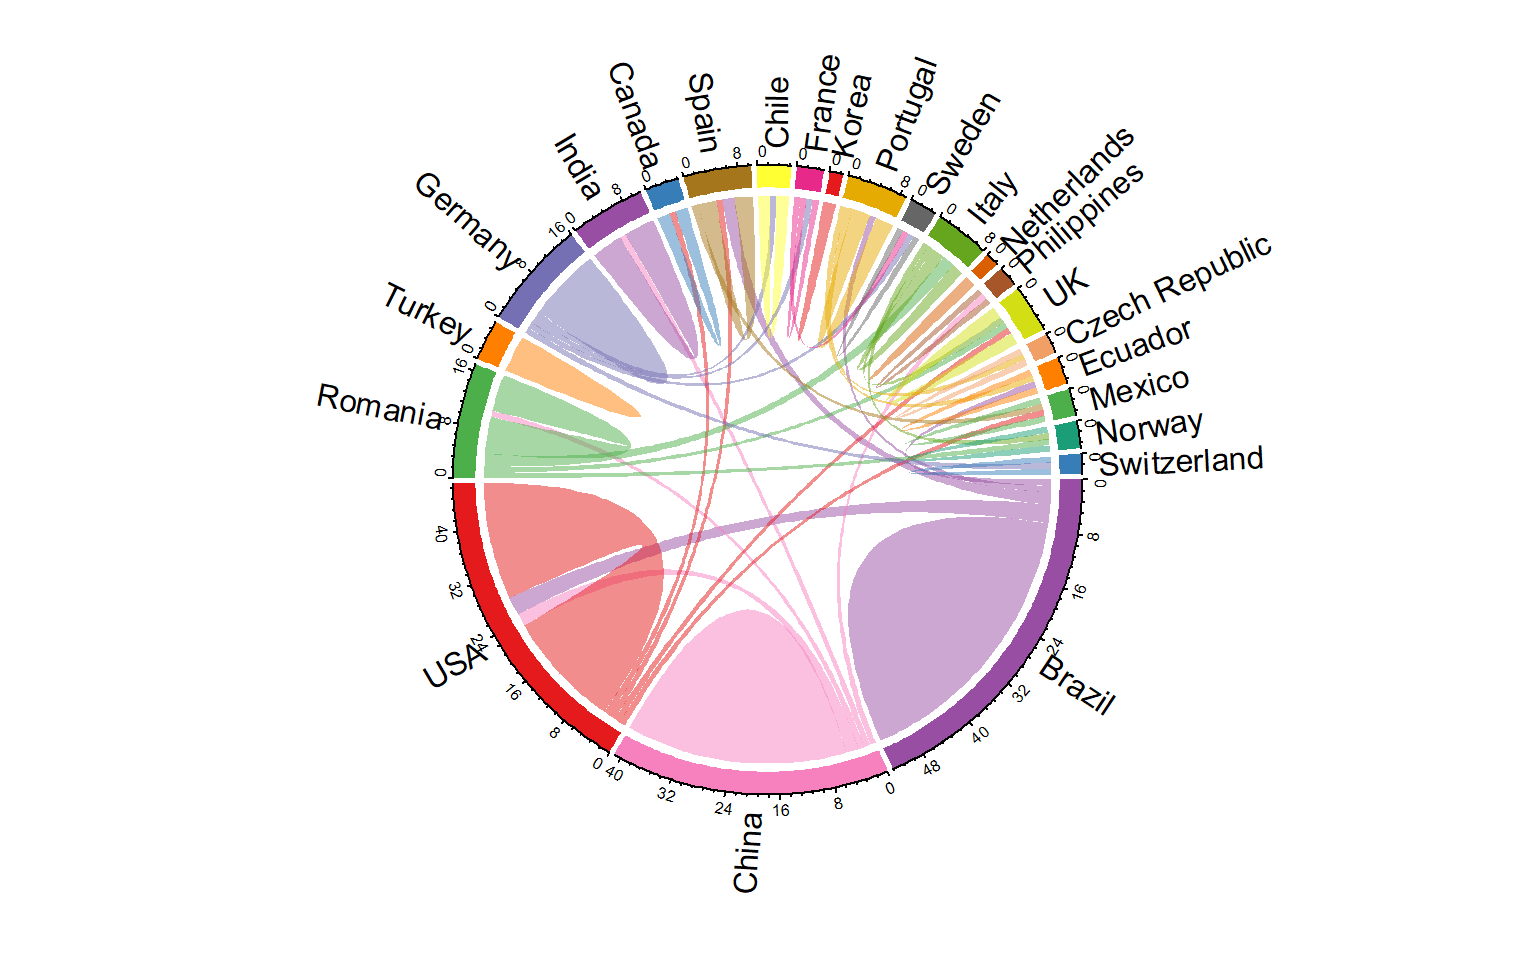
\includegraphics{zf_sm_code_files/figure-latex/unnamed-chunk-37-1.pdf}

\begin{Shaded}
\begin{Highlighting}[]
\CommentTok{\# Create a chord diagram of the network matrix}
\NormalTok{fig6b }\OtherTok{\textless{}{-}} \FunctionTok{chordDiagram}\NormalTok{(merge\_matrix2, }\AttributeTok{annotationTrack =} \StringTok{"grid"}\NormalTok{, }\AttributeTok{preAllocateTracks =} \DecValTok{1}\NormalTok{)}
\CommentTok{\# Add a track to label each sector with its name}
\FunctionTok{circos.trackPlotRegion}\NormalTok{(}\AttributeTok{track.index =} \DecValTok{1}\NormalTok{, }\AttributeTok{panel.fun =} \ControlFlowTok{function}\NormalTok{(x, y) \{}
\NormalTok{  xlim }\OtherTok{=} \FunctionTok{get.cell.meta.data}\NormalTok{(}\StringTok{"xlim"}\NormalTok{)}
\NormalTok{  ylim }\OtherTok{=} \FunctionTok{get.cell.meta.data}\NormalTok{(}\StringTok{"ylim"}\NormalTok{)}
\NormalTok{  sector.name }\OtherTok{=} \FunctionTok{get.cell.meta.data}\NormalTok{(}\StringTok{"sector.index"}\NormalTok{)}
  \FunctionTok{circos.text}\NormalTok{(}\FunctionTok{mean}\NormalTok{(xlim), ylim[}\DecValTok{1}\NormalTok{] }\SpecialCharTok{+} \FloatTok{0.2}\NormalTok{, sector.name, }\AttributeTok{facing =} \StringTok{"clockwise"}\NormalTok{, }\AttributeTok{niceFacing =} \ConstantTok{TRUE}\NormalTok{, }\AttributeTok{adj =} \FunctionTok{c}\NormalTok{(}\DecValTok{0}\NormalTok{, }\DecValTok{1}\NormalTok{))}
  \FunctionTok{circos.axis}\NormalTok{(}\AttributeTok{h =} \StringTok{"top"}\NormalTok{, }\AttributeTok{labels.cex =} \FloatTok{0.5}\NormalTok{, }\AttributeTok{major.tick.length =} \FloatTok{0.2}\NormalTok{, }\AttributeTok{sector.index =}\NormalTok{ sector.name, }\AttributeTok{track.index =} \DecValTok{2}\NormalTok{)}
\NormalTok{\}, }\AttributeTok{bg.border =} \ConstantTok{NA}\NormalTok{)}
\end{Highlighting}
\end{Shaded}

\includegraphics{zf_sm_code_files/figure-latex/unnamed-chunk-37-2.pdf}

\end{document}
